% Options for packages loaded elsewhere
\PassOptionsToPackage{unicode}{hyperref}
\PassOptionsToPackage{hyphens}{url}
\PassOptionsToPackage{dvipsnames,svgnames*,x11names*}{xcolor}
%
\documentclass[
  10pt,
  spanish,
]{book}
\usepackage{amsmath,amssymb}
\usepackage{lmodern}
\usepackage{ifxetex,ifluatex}
\ifnum 0\ifxetex 1\fi\ifluatex 1\fi=0 % if pdftex
  \usepackage[T1]{fontenc}
  \usepackage[utf8]{inputenc}
  \usepackage{textcomp} % provide euro and other symbols
\else % if luatex or xetex
  \usepackage{unicode-math}
  \defaultfontfeatures{Scale=MatchLowercase}
  \defaultfontfeatures[\rmfamily]{Ligatures=TeX,Scale=1}
\fi
% Use upquote if available, for straight quotes in verbatim environments
\IfFileExists{upquote.sty}{\usepackage{upquote}}{}
\IfFileExists{microtype.sty}{% use microtype if available
  \usepackage[]{microtype}
  \UseMicrotypeSet[protrusion]{basicmath} % disable protrusion for tt fonts
}{}
\makeatletter
\@ifundefined{KOMAClassName}{% if non-KOMA class
  \IfFileExists{parskip.sty}{%
    \usepackage{parskip}
  }{% else
    \setlength{\parindent}{0pt}
    \setlength{\parskip}{6pt plus 2pt minus 1pt}}
}{% if KOMA class
  \KOMAoptions{parskip=half}}
\makeatother
\usepackage{xcolor}
\IfFileExists{xurl.sty}{\usepackage{xurl}}{} % add URL line breaks if available
\IfFileExists{bookmark.sty}{\usepackage{bookmark}}{\usepackage{hyperref}}
\hypersetup{
  pdftitle={Diseño y análisis estadístico en las encuestas de hogares de América Latina},
  pdfauthor={Andrés Gutiérrez},
  pdflang={es},
  colorlinks=true,
  linkcolor=blue,
  filecolor=Maroon,
  citecolor=Blue,
  urlcolor=Blue,
  pdfcreator={LaTeX via pandoc}}
\urlstyle{same} % disable monospaced font for URLs
\usepackage{longtable,booktabs,array}
\usepackage{calc} % for calculating minipage widths
% Correct order of tables after \paragraph or \subparagraph
\usepackage{etoolbox}
\makeatletter
\patchcmd\longtable{\par}{\if@noskipsec\mbox{}\fi\par}{}{}
\makeatother
% Allow footnotes in longtable head/foot
\IfFileExists{footnotehyper.sty}{\usepackage{footnotehyper}}{\usepackage{footnote}}
\makesavenoteenv{longtable}
\usepackage{graphicx}
\makeatletter
\def\maxwidth{\ifdim\Gin@nat@width>\linewidth\linewidth\else\Gin@nat@width\fi}
\def\maxheight{\ifdim\Gin@nat@height>\textheight\textheight\else\Gin@nat@height\fi}
\makeatother
% Scale images if necessary, so that they will not overflow the page
% margins by default, and it is still possible to overwrite the defaults
% using explicit options in \includegraphics[width, height, ...]{}
\setkeys{Gin}{width=\maxwidth,height=\maxheight,keepaspectratio}
% Set default figure placement to htbp
\makeatletter
\def\fps@figure{htbp}
\makeatother
\setlength{\emergencystretch}{3em} % prevent overfull lines
\providecommand{\tightlist}{%
  \setlength{\itemsep}{0pt}\setlength{\parskip}{0pt}}
\setcounter{secnumdepth}{5}
\usepackage{setspace}
%\linespread{1.5}
%\usepackage{tikz}
%\usetikzlibrary{shapes,arrows}
\usepackage{pdflscape}
\newcommand{\blandscape}{\begin{landscape}}
\newcommand{\elandscape}{\end{landscape}}
\renewcommand{\thesection}{\Roman{section}}
\renewcommand{\thesubsection}{\Alph{subsection}}
\usepackage{booktabs}
\usepackage{amsthm}
\makeatletter
\def\thm@space@setup{%
  \thm@preskip=8pt plus 2pt minus 4pt
  \thm@postskip=\thm@preskip
}
\makeatother
\usepackage[spanish, spanishkw, onelanguage, linesnumbered]{algorithm2e}
\ifxetex
  % Load polyglossia as late as possible: uses bidi with RTL langages (e.g. Hebrew, Arabic)
  \usepackage{polyglossia}
  \setmainlanguage[]{spanish}
\else
  \usepackage[main=spanish]{babel}
% get rid of language-specific shorthands (see #6817):
\let\LanguageShortHands\languageshorthands
\def\languageshorthands#1{}
\fi
\ifluatex
  \usepackage{selnolig}  % disable illegal ligatures
\fi
\usepackage[]{natbib}
\bibliographystyle{apalike}

\title{Diseño y análisis estadístico en las encuestas de hogares de América Latina}
\author{Andrés Gutiérrez\footnote{Experto regional en estadísticas sociales - Unidad de Estadística Social - Comisión Económica para América Latina y el Caribe (CEPAL) - \href{mailto:andres.gutierrez@cepal.org}{\nolinkurl{andres.gutierrez@cepal.org}}}}
\date{2021-08-05}

\begin{document}
\maketitle

{
\hypersetup{linkcolor=}
\setcounter{tocdepth}{1}
\tableofcontents
}
\listoftables
\listoffigures
\hypertarget{prefacio}{%
\chapter*{Prefacio}\label{prefacio}}
\addcontentsline{toc}{chapter}{Prefacio}

\begin{figure}

\includegraphics[width=100px]{Pics/CClicence} \caption{Licencia de Creative Commons}\label{fig:unnamed-chunk-1}
\end{figure}

La versión online de este libro está licenciada bajo una \href{http://creativecommons.org/licenses/by-nc-sa/4.0/}{Licencia Internacional de Creative Commons para compartir con atribución no comercial 4.0}.

Este libro es el resultado de un compendio de las experiencias internacionales prácticas adquiridas por el autor como Experto Regional en Estadísticas Sociales de la CEPAL.

\hypertarget{resumen}{%
\chapter*{Resumen}\label{resumen}}
\addcontentsline{toc}{chapter}{Resumen}

Las encuestas de hogares son un instrumento necesario para realizar seguimiento a un conjunto amplio de indicadores requeridos para el diseño y evaluación de las políticas públicas. Las encuestas de hogares que se implementan en América Latina son de tipo y características diversas. Aunque los conceptos y procesos para su diseño y análisis guardan similitudes, este documento se enfoca principalmente en los procesos referidos a las encuestas de empleo y de propósitos múltiples, con las que los países estiman los principales indicadores relacionados con el mercado laboral, el nivel y distribución de ingresos y la condición de pobreza y las principales características sociodemográficas de la población. Se realiza un recorrido por los diferentes diseños de muestreo, las metodologías más usadas en la selección de las muestras y las estrategias de estimación de los parámetros de interés. También se revisan las técnicas utilizadas para medir el error de muestreo y los métodos disponibles para encarar desafíos como la ausencia de respuesta y la desactualización de los marcos de muestreo.

\textbf{UNBIS Keywords}. Encuestas por muestreo, encuestas de hogares, indicadores socioeconómicos.

\hypertarget{introducciuxf3n}{%
\chapter{Introducción}\label{introducciuxf3n}}

Las encuestas de hogares son un caso particular de investigación social que indaga acerca de características específicas a nivel del individuo, del hogar o de la vivienda, con el fin de obtener inferencias precisas acerca de constructos de interés. Por su naturaleza, estas investigaciones están relacionadas con variables de salud, educación, ingresos, gastos, situación laboral, acceso y uso de servicios, entre muchas otras. En algunas ocasiones, las encuestas de hogares tienen como objetivo la estimación de uno o varios indicadores que resumen un constructo económico o social. Sin embargo, existe una tendencia creciente de extender las encuestas a constructos más diversos. Es así como cada vez tienen más espacio las encuestas de propósitos múltiples como una fuente relevante de información que permite monitorear indicadores sociales.

En este tipo de encuestas, el hogar es la unidad de análisis, la cual ha sido definida por la División de Estadística de la Organización de las Naciones Unidas \citep{United-Nations_2011} como:

\begin{quote}
\begin{enumerate}
\def\labelenumi{\alph{enumi}.}
\tightlist
\item
  Un grupo de dos o más personas que se combinan para ocupar la totalidad o parte de una vivienda y para proporcionarse alimentos y posiblemente otros artículos esenciales para la vida. El grupo puede estar compuesto solo de personas relacionadas o de personas no relacionadas o de una combinación de ambos. El grupo también puede compartir sus ingresos.
\item
  Una persona que vive sola en una vivienda separada o que ocupa, como huésped, una habitación (o habitaciones) separada de una vivienda pero que no se une a ninguno de los otros ocupantes de la vivienda para formar parte de una hogar de múltiples personas.
\end{enumerate}
\end{quote}

Nótese que la anterior definición refleja la dinámica natural del cambio en las poblaciones de hogares, por lo cual se deben tener distintos enfoques para abordar el problema de la medición de indicadores sociales. En América Latina, existen una gran variedad de encuestas que abordan diferentes problemáticas sociales. Todas y cada una de ellas han sido diseñadas cuidadosamente para que respondan a las necesidades de la sociedad. Este documento plantea una recopilación de las técnicas usadas tanto en su diseño, como en su análisis.

No todas las encuestas se diseñan de la misma forma y por ende debe haber una distinción entre ellas. Por ejemplo, \citet{Kalton_Citro_1993} afirman que las encuestas de hogares pueden clasificarse en varios tipos:

\begin{itemize}
\tightlist
\item
  \emph{Encuestas repetidas}, definidas como una serie de encuestas transversales aplicadas en diferentes momentos del tiempo con el mismo diseño metodológico, en donde la selección de hogares se hace de forma independiente para cada aplicación.
\item
  \emph{Encuestas tipo panel}, para las cuales los datos son recolectados en diferentes momentos del tiempo utilizando la misma muestra de hogares en el tiempo.
\item
  \emph{Encuestas rotativas}, en donde un porcentaje de hogares se mantiene en un periodo de tiempo respondiendo la encuesta y en cada aplicación algunos hogares son reemplazados por nuevos hogares de forma planificada.
\end{itemize}

El diseño de la encuesta dependerá sistemáticamente del objetivo de la medición. Por ejemplo, \citet{Kalton_2009} afirma que es prudente hacer un buena inversión en el desarrollo e implementación de un buen diseño para amortizar los costos de todo el estudio. Por lo tanto, lo que se quiere al diseñar una encuesta de hogares es que sea un instrumento confiable, que brinde estimaciones exactas y precisas, puesto que de lo contrario no se podrían monitorear las políticas públicas y los indicadores de interés de forma consistente. Por ejemplo, uno de los indicadores sociales con mayor impacto es la tasa de desocupación, que mide la razón entre la cantidad de personas que se encuentran desocupados, pero que forman parte del mercado de trabajo. Las encuestas de empleo tienen características particulares, diferentes a las de las encuestas que miden otro tipo de constructos. \citet{Duncan_Kalton_1987} mencionan que las encuestas de hogares pueden proveer estimaciones de los parámetros poblacionales en distintos puntos del tiempo, por ejemplo, la estimación de la tasa de desocupación mensual; proveer estimaciones del cambio neto de los parámetros poblacionales entre periodos de tiempo, por ejemplo, el cambio en la tasa de desocupación entre dos periodos consecutivos; o incluso medir varios componentes de cambio individual, por ejemplo cambios brutos en la situación laboral de los jefes de hogar, para lo cual se requiere que la encuesta contemple un diseño de panel o de panel rotativo.

\hypertarget{objetivos-de-desarrollo-sostenible}{%
\subsection*{Objetivos de Desarrollo Sostenible}\label{objetivos-de-desarrollo-sostenible}}
\addcontentsline{toc}{subsection}{Objetivos de Desarrollo Sostenible}

La medición de los indicadores en el mercado de trabajo es sólo un pequeño componente en el basto universo de posibilidades de medición que brindan las encuestas de hogares. Por esta razón, este tipo de levantamientos se ha convertido en una herramienta fundamental para medir indicadores sociales en todo el mundo y que, en particular, permiten que las naciones de América Latina puedan hacer seguimiento a su desarrollo económico y social. Sin embargo, este tipo de instrumentos puede ser utilizado como herramienta para monitorear el progreso de los países en términos de metas y objetivos comunes. Es así como en 2015, la Asamblea General de la Organización de las Naciones Unidas aprobó una resolución que plantea un plan de acción en favor de las personas, el planeta y la prosperidad \citep{United_Nations_2015}. Esa resolución propone el seguimiento de 17 Objetivos de Desarrollo Sostenible (\href{https://sustainabledevelopment.un.org}{ODS}) y 169 metas de carácter integrado e indivisible que se conjugan en las dimensiones económica, social y ambiental. Para realizar el seguimiento a los ODS es posible utilizar diferentes fuentes de información, como censos, registros administrativos, registros estadísticos, proyecciones demográficas y también las encuestas de hogares \citep{United_Nations_2016}. En particular, cada una de las metas de los ODS contiene indicadores, muchos de los cuales no pudieran ser estimados de no ser por la información disponible en las encuestas de hogares.

Por ejemplo, el objetivo \textbf{8} busca \emph{promover el crecimiento económico sostenido, inclusivo y sostenible, el empleo pleno y productivo y el trabajo decente para todos}. Claramente de este objetivo se desprenden indicadores que permiten conocer la evolución de los países en la consecución de las metas. Dentro de este objetivo, se encuentra la meta \textbf{8.6} que apunta a reducir sustancialmente la proporción de jóvenes sin empleo y sin educación o entrenamiento. Esta meta se mide con el indicador \textbf{8.6.1} definido como la proporción de jóvenes (entre 15 y 24 años de edad) sin educación y sin empleo.

\hypertarget{mercado-de-trabajo}{%
\subsection*{Mercado de Trabajo}\label{mercado-de-trabajo}}
\addcontentsline{toc}{subsection}{Mercado de Trabajo}

Desde otra perspectiva, en el marco de la Decimotercera Conferencia Internacional de Estadísticos del trabajo en 1982, la Organización Internacional del Trabajo (OIT) adoptó algunas directrices concernientes con la medición y análisis de estadísticas oficiales de la fuerza de trabajo, del empleo y del desempleo con miras a mejorar la comparabilidad de las cifras y mejorar su utilidad en los países \citep{OIT_1982}. En esta resolución se hace un énfasis especial en que las encuestas de hogares constituyen un medio apropiado de recopilación de datos sobre la población económicamente activa y que la planeación de estas investigaciones en los países debería ceñirse a las normas internacionales. Por consiguiente, la resolución afirma que las encuestas de hogares deberían:

\begin{enumerate}
\def\labelenumi{\arabic{enumi}.}
\tightlist
\item
  Brindar datos de la población económicamente activa, definida por las personas en edad laboral que se han integrado al mercado de trabajo (trabajadores o peersonas en búsqueda de empleo).
\item
  Proveer estadísticas básicas de sus actividades durante el año, así como las relaciones entre el empleo, ingreso y otras características económicas y sociales.
\item
  Proveer datos sobre otros temas particulares para responder a las necesidades a largo plazo y de índole permanente.
\end{enumerate}

En el año 2013, la OIT decidió revisar esta resolución y propuso algunos cambios en el marco de la 19 Conferencia Internacional de Estadísticos del Trabajo en donde se acogieron algunas modificaciones en términos de los objetivos de medición y el alcance de los sistemas nacionales de estadísticas del trabajo, el concepto de trabajo en todas sus formas, el empleo, la medición de las personas en situación de subutilización de la fuerza de trabajo, métodos de recopilación de datos, entre otras \citep{OIT_2013}. Es así como las Oficinas Nacionales de Estadística (ONE) de América Latina no sólo planean las encuestas de hogares de tal forma que puedan responder a los nuevos retos en términos de la estimación de los parámetros de interés en cuanto al trabajo remunerado o no remunerado para mantener la comparabilidad de las estadísticas laborales entre los países, proporcionando nuevos y mejores indicadores para contribuir al análisis de la dinámica del mercado laboral, sino que se actualizan paulatinamente para poder brindar la información que la sociedad necesita a medida que evoluciona el constructo social de interés.

\hypertarget{ingresos-y-gastos}{%
\subsection*{Ingresos y gastos}\label{ingresos-y-gastos}}
\addcontentsline{toc}{subsection}{Ingresos y gastos}

Es importante resaltar que los indicadores de bienestar (en términos de ingresos y gastos) también hacen parte del conjunto de parámetros que se pueden estimar desde las encuestas de hogares. Medir el ingreso a partir de las encuestas de hogares se constituye en un reto metodológico para los institutos nacionales de estadística en el mundo, y particularmente en América Latina. Es recomendable seguir las directrices de la Comisión Económica para Europa que revisten una actualización de los estándares internacionales, recomendaciones y buenas prácticas en la medición del ingreso en los hogares. Por ejemplo, el llamado Grupo de Canberra ha revisado exhaustivamente el tópico de la estimación del ingreso estudiando las prácticas de algunos países en términos del aseguramiento de la calidad y la publicación de este tipo de estadísticas oficiales y ha provisto la siguiente definición de ingreso en el hogar \citep{United-Nations_2011}:

\begin{quote}
\emph{El ingreso del hogar se compone de las entradas monetarias, en especie o en servicios que por lo general son frecuentes y regulares, están destinadas al hogar o a los miembros del hogar por separado y se reciben a intervalos anuales o con mayor frecuencia. Durante el período de referencia en el que se reciben, tales entradas están potencialmente disponibles para el consumo efectivo y, habitualmente, no reducen el patrimonio neto del hogar.}
\end{quote}

Con base en lo anterior, el uso de las encuestas de hogares para estimar el ingreso reviste retos metodológicos mayores puesto que los entrevistados deben responder con precisión cuando se les indague por este constructo que contiene los ingresos personales de cada individuo en el hogar, como sueldos y salarios, ganancias, ingresos del empleo, pensiones, etc. y también los ingresos del hogar, incluidas las rentas por alquiler y los ingresos generados por el comercio. Por lo tanto, el diseño de la encuesta debe tener en cuenta la definición de un instrumento que sea relevante para el respondiente y le permita identificar y, en algunas ocasiones, recordar la información con un cierto grado de exactitud.

Por ejemplo, si el respondiente es empleado regular, el instrumento de medición debería planearse de tal manera que el entrevistado pueda recordar la información de interés, como los rubros de seguridad social hechos por su empleador. Por otro lado, si se requiere que el respondiente brinde información acerca de un determinado periodo de tiempo, el planteamiento de la pregunta, la forma de indagar y el entrenamiento de los encuestadores pueden sesgar sistemáticamente la respuesta y por consiguiente inducir estimaciones poco confiables. Mucho se ha investigado al respecto de cómo realizar preguntas certeras en este tipo de levantamientos y el lector interesado puede consultar los trabajos de \citet{Biemer_Lyberg_2003}, \citet{Presser_Rothgeb_Couper_Lessler_Martin_Martin_Singer_2004}, y \citet{Groves_Fowler_Couper_Lepkowski_Singer_Tourangeau_2009}.

\hypertarget{esquema-del-documento}{%
\subsection*{Esquema del documento}\label{esquema-del-documento}}
\addcontentsline{toc}{subsection}{Esquema del documento}

Este documento pretende revisar algunas de las metodologías más usadas por las ONE de América Latina en cuanto al diseño y análisis estadístico de las encuestas de hogares y puede servir de guía técnica a los estadísticos de la región que se encuentran involucrados en los procesos técnicos de este tipo de encuestas. De la misma forma, este documento considera conjuntamente los dos principales momentos de las encuestas: el diseño y el análisis. Nótese que estos momentos están escindidos por el levantamiento de la información en campo y parten la realización de la encuesta en dos. Los lectores que están familiarizados con la investigación social a través de las encuestas de hogares encontrarán que estas operaciones estadísticas se planean teniendo en cuenta muchos pormenores que podrían suceder en campo. Es por esto que el trabajo de las encuestas asciende cuando se logra plasmar la información recolectada en una de base de datos. En este segundo momento es cuando se debe asegurar que lo que se planificó efectivamente sea incorporado en el análisis de esta información. Desde esta perspectiva, este documento puede verse en dos momentos: los capítulos 2, 3 y 4 abordan el diseño, mientras que los capítulos 4, 5 y 6 y 7 abordan el análisis. Esta distinción así como los procesos que la componen se presenta en la Figura \ref{fig:esquema}.

\begin{figure}
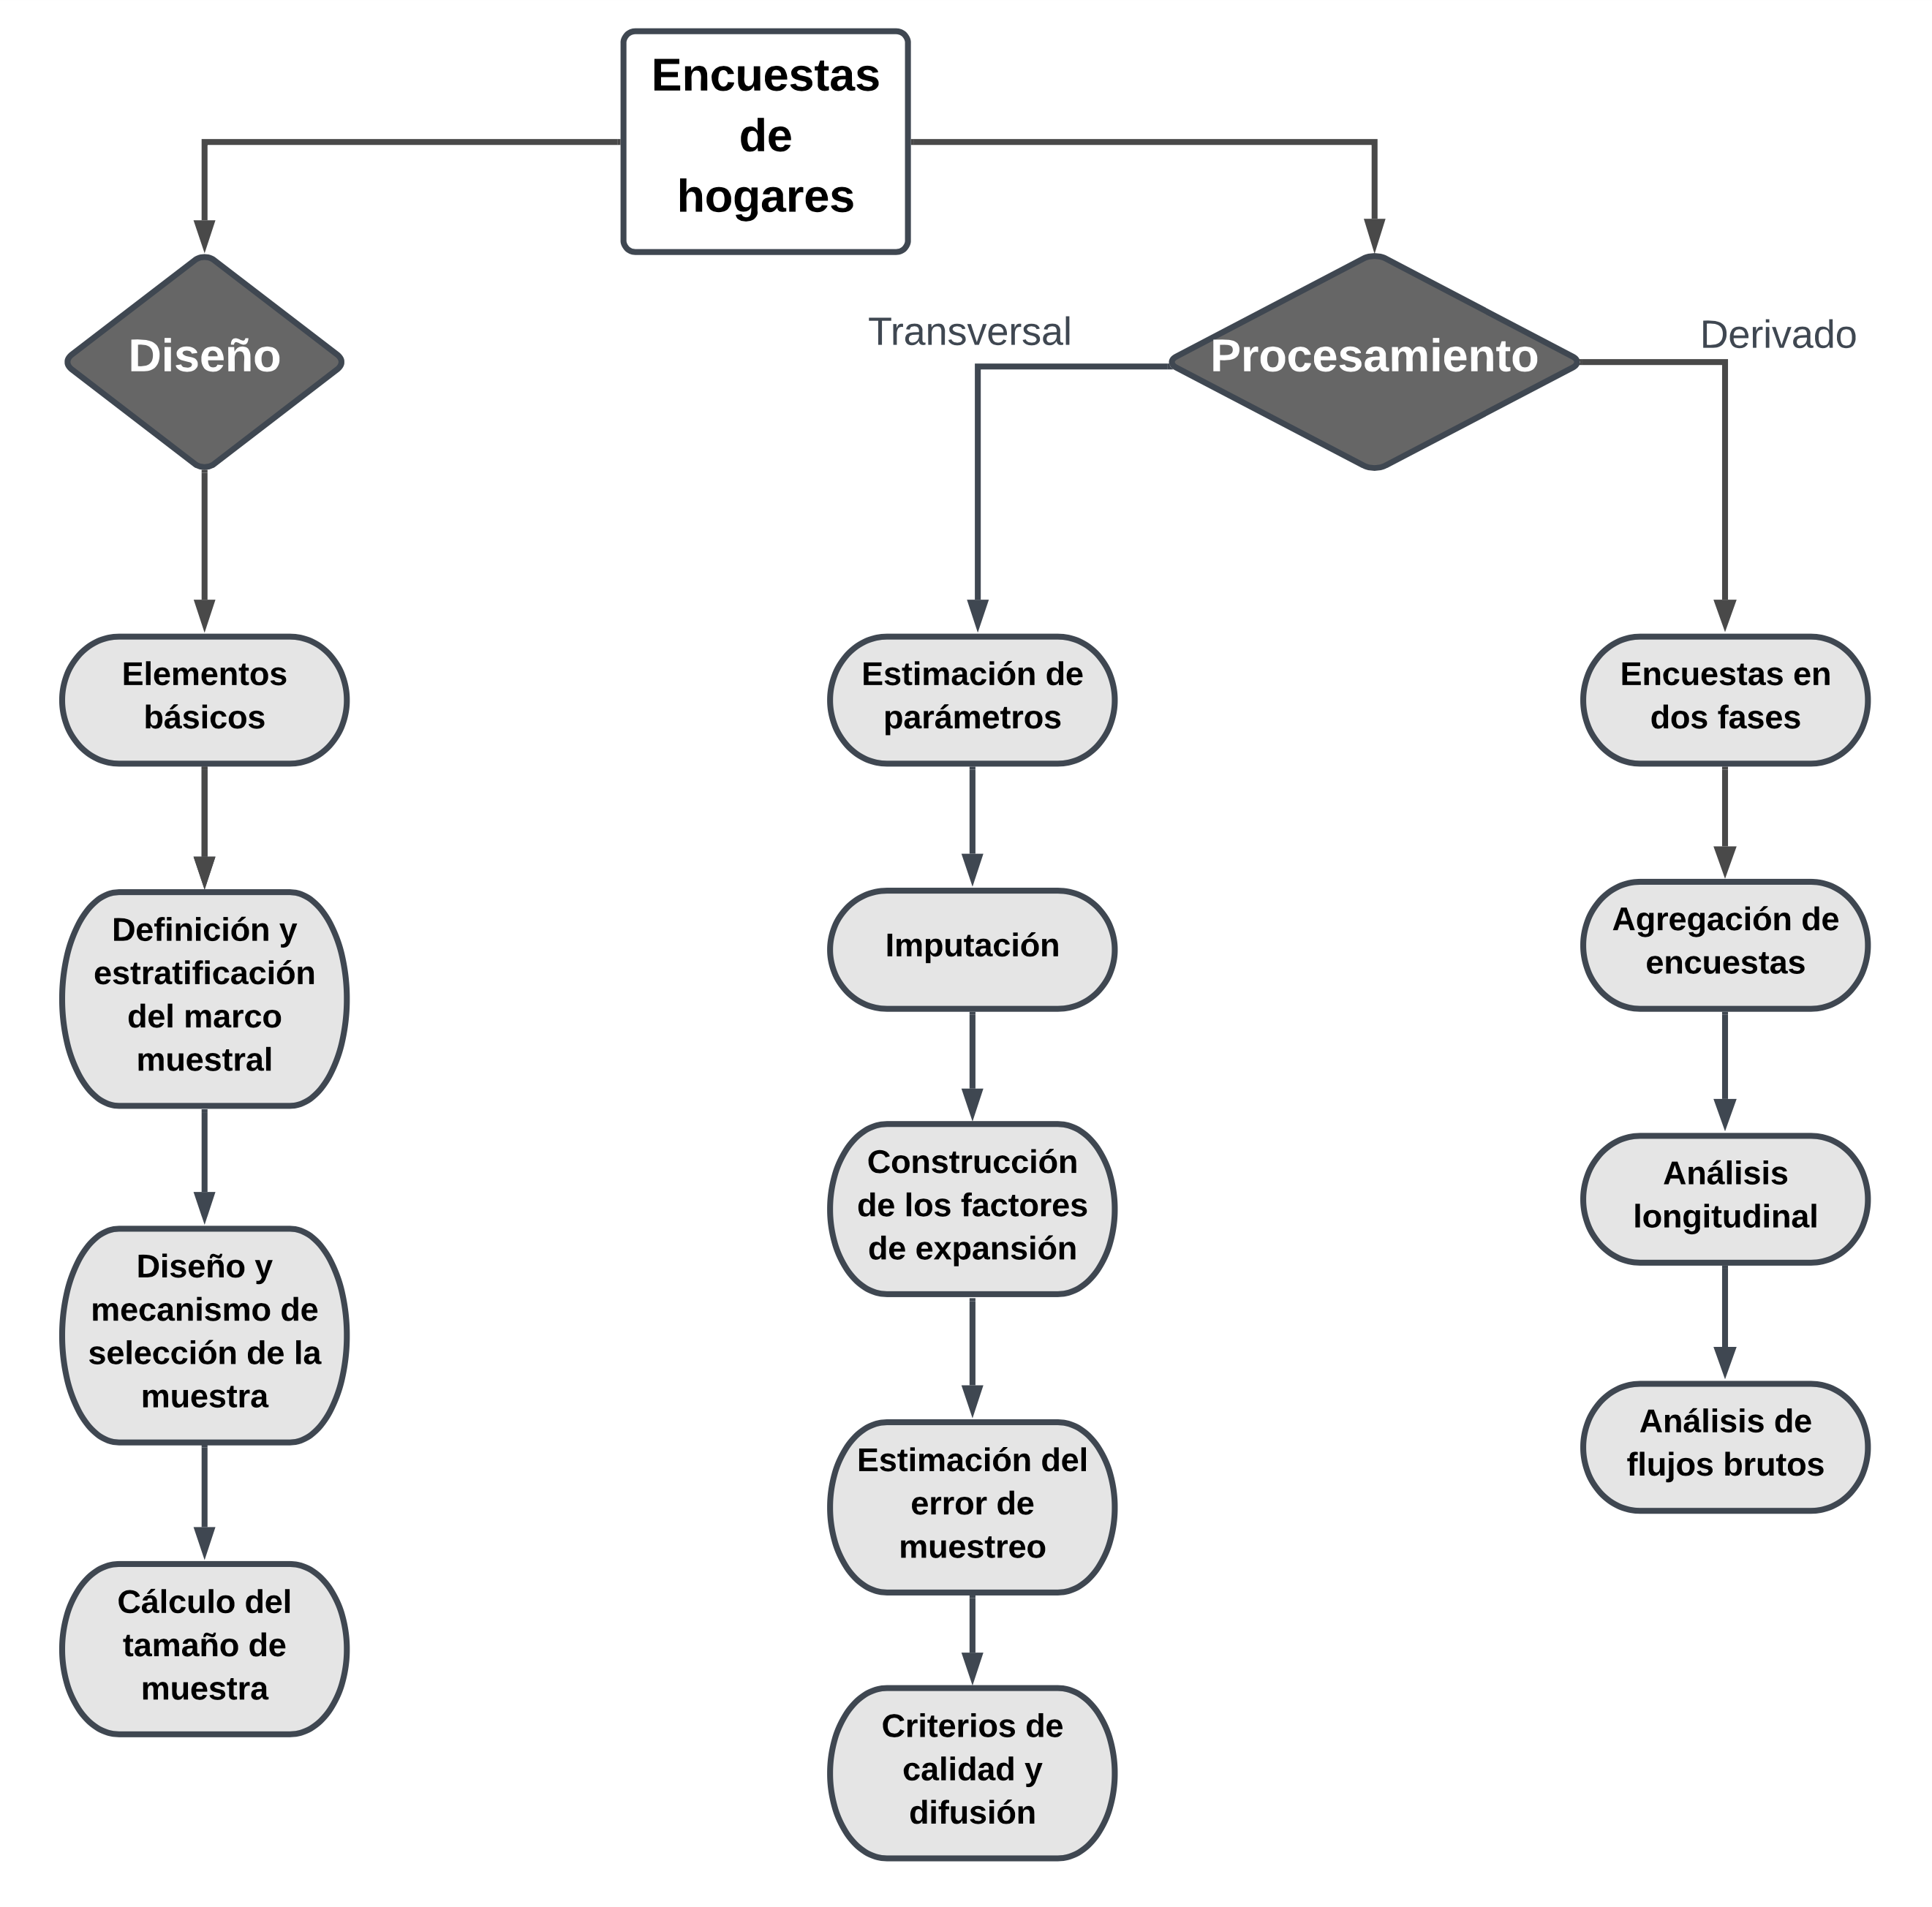
\includegraphics[width=700px]{Pics/Intro} \caption{Esquema de procesos en el análisis y diseño de una encuesta de hogares.}\label{fig:esquema}
\end{figure}

En el primer capítulo se considera una breve introducción a la problemática de las encuestas de hogares. En el capítulo dos se aborda con más detalle los elementos básicos que se consideran por lo regular en los diseños de las encuestas de hogares. Un aspecto relevante de este documento es que, si bien considera que las encuestas de hogares tienen muchos elementos en común, diferencia de forma cuidadosa las particularidades de cada encuesta. Por ejemplo, en este capítulo se trata el tema del diseño de las encuestas rotativas y se profundiza en los diferentes parámetros que se pueden considerar en este tipo de operaciones; asimismo, describe las características metodológicas que se deben considerar al momento de diseñar la encuesta y revisa los conceptos esenciales que determinarán el tipo de aplicación que se debe considerar. El capítulo tres describe los principales diseños de muestreo que se utilizan en este tipo de estudios y expone de forma estándar los conceptos de estratificación y aglomeración de las poblaciones. El capítulo cuatro complementa estos conceptos con varias aplicaciones prácticas para determinar el tamaño de muestra adecuado para lograr los objetivos de la investigación. A pesar de que la literatura relacionada con la práctica del muestreo es relativamente abundante, existen pocos ejemplos prácticos que logren representar la problemática del tamaño de muestra y el lector podrá encontrar herramientas ilustrativas basadas en múltiples escenarios de la problemática social.

Pasando a la parte del análisis de las encuestas, el capítulo cinco revisa los procesos de imputación y ponderación en la encuesta. Los procesos de imputación tratan de recuperación tanta información como sea posible para que el investigador pueda contar con una base de datos rectangular y completa. Luego de esto, es necesario aplicar los factores de expansión a la información contenida en la base de datos para que se puedan realizar inferencias a nivel nacional o regional. Sin embargo, en aquellos casos en donde la imputación no resulta ser una técnica adecuada para completar la información faltante, es necesario realizar ajustes sistemáticos en los factores de expansión para que la muestra efectiva siga siendo una muestra representativa de toda la población. El capítulo seis analiza las principales metodologías de estimación, tanto de los parámetros de interés como de sus errores de muestreo. Si hay algo que distingue el análisis de las encuestas de cualquier otro tipo de estudio estadístico es que las propiedades importantes como insesgamiento, consistencia y eficiencia están basadas en el diseño de muestreo y no en supuestos metodológicos ligados a algún modelo estocástico. Es por esto que se presta especial atención a la estimación del error de muestreo, que no es otra cosa que una función de la varianza de las estimaciones, y se presentan las metodologías más comunes en términos de aproximaciones teóricas y computacionales al error de muestreo. El capítulo siete presenta de forma detallada los procesos que se surten cuando se agregan encuestas a lo largo de un periodo de tiempo. Acudiendo a la perspectiva del autor, el capítulo ocho presenta los criterios de calidad que se deberían tener en cuenta para decidir si una cifra, resultante de un proceso de estimación estadística basada en encuestas de hogares, debería ser o no publicada a la sociedad. Por úlitmo, el capítulo nueve presenta una discusión acerca del uso presente de las encuestas de hogares y los retos que depara el futuro en materia de la medición de indicadores sociales a través de las encuestas de hogares. Asimismo, en los anexos se contempla una revisión del software que se utiliza actualmente en los ONE para llevar a cabo esta ardua tarea de diseñar y analizar las encuestas de hogares, una revisión rápida de algunas de las encuestas de la región, así como algunas directrices que se deberían considerar al momento de documentar los procesos asociados a las encuestas de hogares.

\hypertarget{part-diseuxf1o-estaduxedstico-de-las-encuestas-de-hogares}{%
\part{Diseño estadístico de las encuestas de hogares}\label{part-diseuxf1o-estaduxedstico-de-las-encuestas-de-hogares}}

\hypertarget{el-paradigma-del-error-total}{%
\chapter{El paradigma del error total}\label{el-paradigma-del-error-total}}

Todos los procesos en la encuesta deben estar planificados y probados de antemano, antes de la recolección de los datos. Por ejemplo, el cuestionario debe estar muy bien diseñado para que las respuestas de las personas describan acertadamente las características de los entrevistados. De la misma forma, el subconjunto de personas que participan en la encuesta debe ser expandido con precisión y confiabilidad a la población de interés.

En una encuesta, el interés no se centra en las características particulares de un individuo sino en las características de la población a la cual ese individuo pertenece. De esta forma, la inferencia siempre se realiza teniendo en mente agregados (indicadores) poblacionales. Existen muchas fuentes de error\footnote{Error no necesariamente significa equivocación.} cuando se realiza una encuesta.

\begin{enumerate}
\def\labelenumi{\arabic{enumi}.}
\tightlist
\item
  \textbf{Error de muestreo}: ocurre porque no se incluyeron a todas las personas de la población y se seleccionó una muestra.
\item
  \textbf{Error no muestral}: se refiere a las posibles desviaciones de las respuestas provistas por un entrevistado con respecto al verdadero atributo que se desea medir.
\end{enumerate}

\begin{figure}
\centering
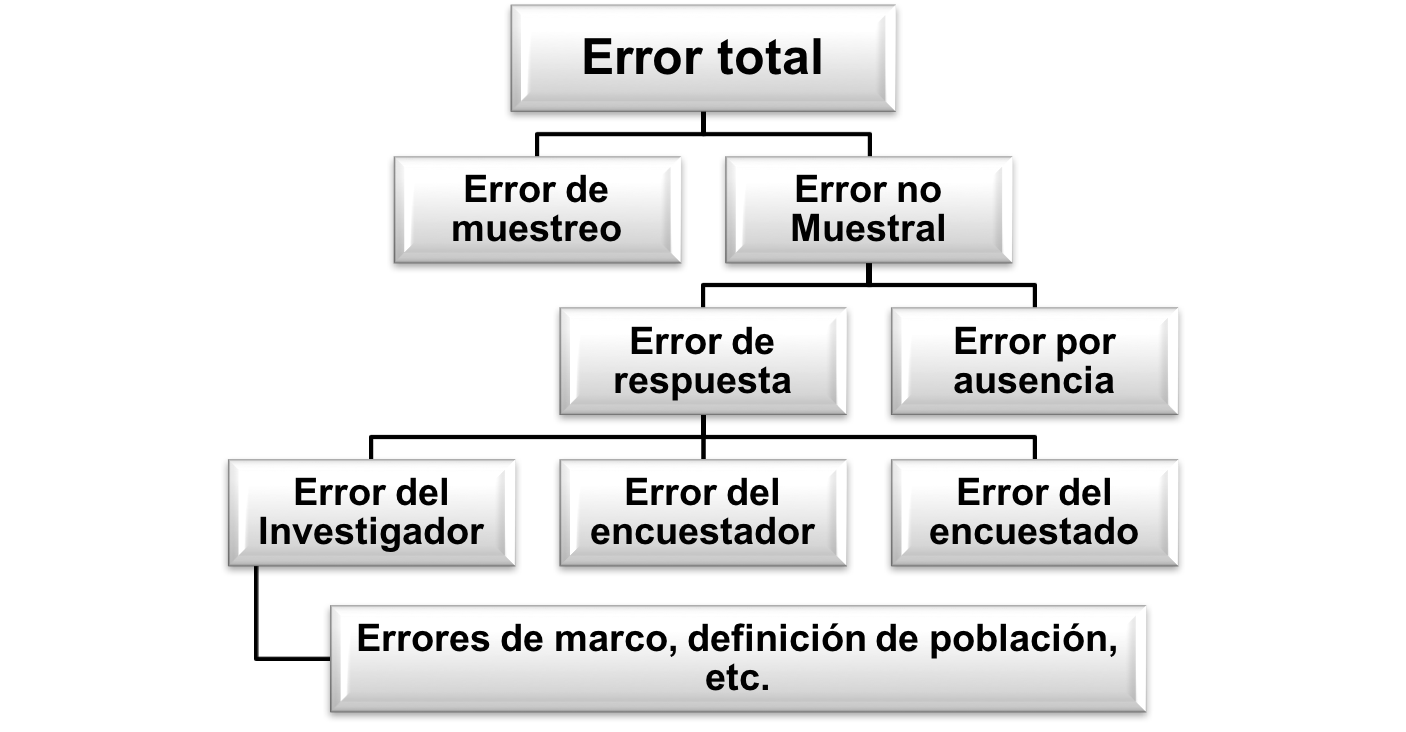
\includegraphics{Pics/Picture9.png}
\caption{\emph{El paradignma del error total.}}
\end{figure}

Por ejemplo, en una encuesta de fuerza laboral mensual, puede haber confusión en el respondiente si no se hace hincapíe en el periodo de referencia (la semana pasada), además pueden existir no respondientes, o el marco puede estar desactualizado. Uno de los objetivos de la planeación concienzuda de la encuesta es minimizar los errores no muestrales. Es necesario minimizar las discrepancias encontradas entre la respuesta verdadera a una pregunta y la respuesta final.

\citet{Groves_Fowler_Couper_Lepkowski_Singer_Tourangeau_2009} plantea que durante todo el siglo pasado, ha surgido una serie de teorías y principios que ofrecen un marco de referencia unificado en el diseño, implementación y evaluación de encuestas. Este marco de referencia se conoce comúnmente como el paradigma del error total de muestreo y ha encaminado la investigación moderna hacia una mejor calidad de las encuestas.

\hypertarget{quuxe9-es-una-encuesta}{%
\section{¿Qué es una encuesta?}\label{quuxe9-es-una-encuesta}}

\citet{Groves_Fowler_Couper_Lepkowski_Singer_Tourangeau_2009} afirma que una encuesta es un método sistemático para obtener información de (una muestra de) entes, con el fin de construir descriptores cuantitativos de los atributos de una población más grande, de la cual los entes son miembros.
Por otro lado, Wikipedia afirma que una encuesta es un estudio observacional en el cual el investigador busca recaudar datos por medio de un cuestionario pre-diseñado, y no modificar el entorno ni controlar el proceso que está en observación (como sí lo hace en un experimento).

Además, los datos se obtienen a partir de realizar un conjunto de preguntas normalizadas dirigidas a una muestra representativa o al conjunto total de la población estadística en estudio, formada a menudo por personas, empresas o entes institucionales, con el fin de conocer estados de opinión, características o hechos específicos. Hay una diferencia sustancial entre los sondeos y las encuestas; de esta forma,

\begin{itemize}
\tightlist
\item
  \textbf{Sondeo}: es la traducción de \emph{poll}, que a su vez viene del antiguo alemán referente a cabeza y se utilizaba para contar: ``contar cabezas''.
\item
  \textbf{Encuesta}: es la traducción de \emph{survey}, que a su vez viene del latín \emph{super} (sobre) y \emph{videre} (observar).
\end{itemize}

En general, la primera expresión aparece muchas más veces en el sector privado, en estudios de opinión y de consumo. Un sondeo no será jamás utilizado para obtener estadísticas oficiales en estudios gubernamentales o en dominios científicos. Sin embargo, los sondeos muchas veces opacan la perspectiva científica de las cifras y pueden llevar a conclusiones inexactas acerca de la realidad de una problemática. Muchos procesos de recolección de información se hacen llamar encuestas. Para efectos de este documento, una encuesta tendrá las siguientes características:

\begin{enumerate}
\def\labelenumi{\arabic{enumi}.}
\tightlist
\item
  Los datos son recopilados mediante preguntas a personas.
\item
  Las respuestas son compiladas cuando: a) un encuestador pregunta y graba las respuestas del entrevistado o b) el encuestado lee y graba sus propias respuestas.
\item
  Los datos son recolectados de un subgrupo de personas pertenecientes a la población de interés
\end{enumerate}

\hypertarget{evoluciuxf3n-de-las-encuestas-estandarizadas}{%
\section{Evolución de las encuestas estandarizadas}\label{evoluciuxf3n-de-las-encuestas-estandarizadas}}

Cuando el mundo occidental dejó de lado los grandes traumatismos del siglo XX, la investigación social tuvo un auge sobresaliente. Desde entonces, existen tres preguntas, en continua dinámica, que se deben responder para realizar una encuesta:

\begin{itemize}
\tightlist
\item
  ¿Cómo se diseñan las preguntas?
\item
  ¿Cómo se selecciona la muestra?
\item
  ¿Cómo se recolectan los datos?
\end{itemize}

\hypertarget{inicio-de-los-cuestionarios-estandarizados}{%
\subsubsection*{Inicio de los cuestionarios estandarizados}\label{inicio-de-los-cuestionarios-estandarizados}}
\addcontentsline{toc}{subsubsection}{Inicio de los cuestionarios estandarizados}

La práctica de realizar las mismas preguntas en forma de cuestionario es reciente. En el principio cada encuestador preguntaba \emph{lo mismo}, pero con diferentes palabras. Difícilmente, dos personas distintas eran entrevistadas con las mismas preguntas. Se encontró que la forma en cómo se preguntaba y cómo se recopilaba la información afectaba dramáticamente los resultados de las encuestas. Fue así como se decidió que los encuestadores deberías ser entrenados (pre-operativo) formalmente.

Desde la psicometría se implementó el formalismo del cuestionario. Intentando medir estados psicológicos, afectivos e intelectuales, se desarrollaron técnicas primitivas para hacer comparables las respuestas. Likert (1932) demostró que era posible realizar este tipo de comparaciones, evadiendo los largos instrumentos de medición, al formular una sola pregunta - a todos los encuestados - con una serie de respuestas en forma de escala.

\hypertarget{inicio-de-los-muxe9todos-de-muestreo}{%
\subsubsection*{Inicio de los métodos de muestreo}\label{inicio-de-los-muxe9todos-de-muestreo}}
\addcontentsline{toc}{subsubsection}{Inicio de los métodos de muestreo}

En un principio, los investigadores trataban de recolectar datos sobre todos los elementos de la población de interés. Esta práctica resultaba logísticamente inadecuada cuando se trataba de poblaciones con un gran tamaño. Los cálculos de los indicadores sobre toda una población resultaban muy demandantes. Aunque la teoría de la probabilidad tuvo sus orígenes en el siglo XVIII, no fue hasta la segunda década del siglo XX que se utilizó para realizar encuestas. La primera aplicación fue la selección sistemática de un elemento entre un conjunto de N. Para realizar esta selección, los registros censales se dividían en secciones y se procedía a seleccionar un elemento de la sección.

Más adelante, cuando la estadística permeó la agricultura, se definieron otros tipos de muestreo (menos demandantes) y se dio origen al muestreo de áreas. Es así como hoy en día es posible seleccionar muestras de bloques, manzanas, UPZ, secciones y sectores cartográficos. Se descubrió que era posible generalizar el muestreo de áreas y se creó el muestreo multietápico que permitió la selección de grandes bloques dentro de una ciudad, y áreas dentro de los bloques y el submuestreo sucesivo de unidades dentro hasta llegar a la unidad de interés. Todos estos submuestreos se realizan de forma probabilística.

La segunda guerra mundial y la gran depresiones en EE.UU. fueron catalizadores de las encuestas a gran escala. En ese entonces, al igual que hoy, la tasa de desempleo era una cifra importante. Las políticas públicas empezaron a decidirse de acuerdo con las estadísticas oficiales. Las grandes encuestas se realizaron mensualmente. Hoy en día existen cientos de encuestas mensuales que dan cuenta de la realidad de las sociedades.

\hypertarget{inicio-de-la-recolecciuxf3n-de-datos}{%
\subsubsection*{Inicio de la recolección de datos}\label{inicio-de-la-recolecciuxf3n-de-datos}}
\addcontentsline{toc}{subsubsection}{Inicio de la recolección de datos}

Debido a que en un principio no existía un cuestionario estandarizado, entonces las respuestas abiertas eran la única opción de recopilar información. Esta práctica demandaba un gran esfuerzo en términos de resumir y sintetizar todo el corpus de palabras que los entrevistados usaban para responder.

En EE.UU. se dio un fenómeno en la mitas de los años 1960's: la proliferación de las entrevistas por correo. Los países con registros administrativos actualizados pueden contemplar este escenario puesto que induce una altas tasas de cobertura a precios más económicos (pues se prescinde del encuestador). Las bajas tasas de respuestas (pues el encuestado debe llenar un formulario con sus respuestas y devolverlo a la oficina postal) hicieron que paulatinamente esta forma de recolección no fuese tan apetecida.

Un camino intermedio entre las entrevistas cara a cara y las formularios auto-administrados por correo postal son las entrevistas telefónicas. Hoy en día, la mayoría de encuestas en investigación de medios y de mercado se realiza por teléfono.

\hypertarget{el-ciclo-de-vida-de-una-encuesta}{%
\section{El ciclo de vida de una encuesta}\label{el-ciclo-de-vida-de-una-encuesta}}

Atendiendo al modelo de \citet{Groves_Fowler_Couper_Lepkowski_Singer_Tourangeau_2009}, se puede afirmar que en todas la encuestas se tienen dos niveles de inferencia: el individual y el grupa. El proceso de inferencia individual trata con los mismos respondientes que proveen la información primaria en el estudio; mientras que el el proceso de inferencia grupal, basado en una aproximación inductiva, va desde lo particular (la muestra) a lo general (la población).
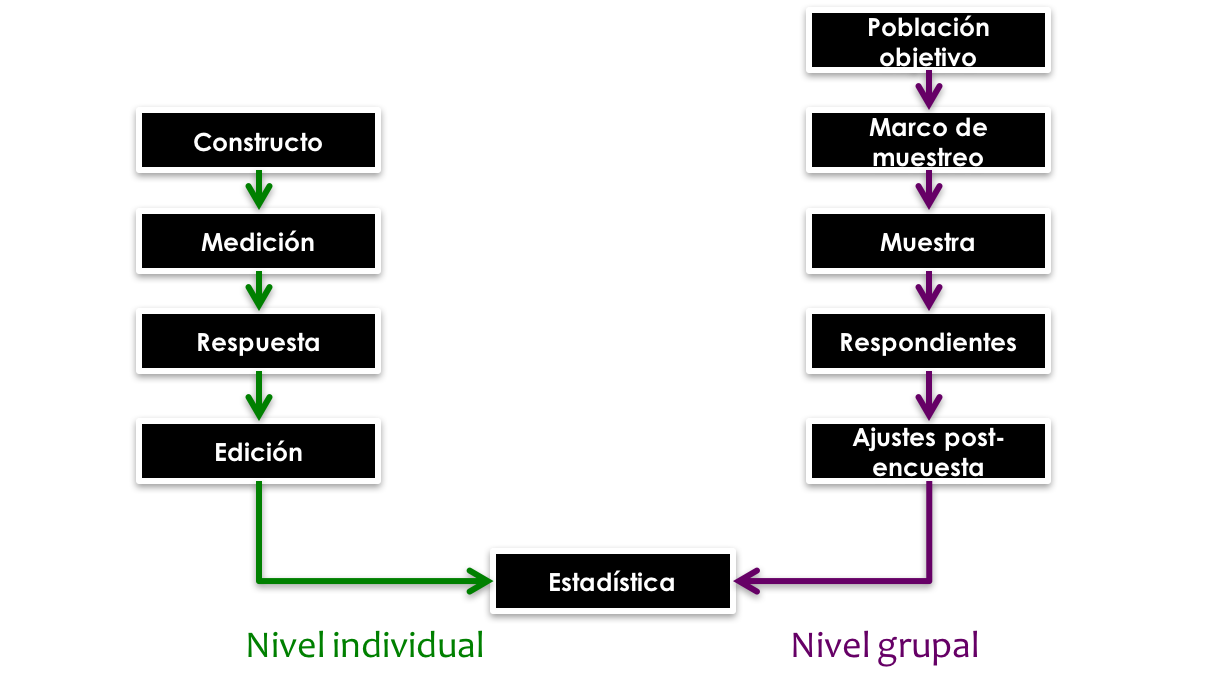
\includegraphics{Pics/Picture6.png}

\hypertarget{inferencia-individual}{%
\subsection{Inferencia individual}\label{inferencia-individual}}

\hypertarget{constructo}{%
\subsubsection*{Constructo}\label{constructo}}
\addcontentsline{toc}{subsubsection}{Constructo}

Los constructos son las ideas abstractas (ambiguas) sobre las cuales el investigador desea inferir y que, a su vez, dan origen a la investigación al ser la simiente de la encuesta. Las palabras con que se describen los constructos son siempre simples, pero la redacción elaborada de los constructos no siempre es precisa. Por ejemplo:

\begin{itemize}
\tightlist
\item
  En una \emph{encuesta de victimización} que mida la cantidad de incidentes relacionados con crímenes en un año determinado, es necesario definir muy apropiadamante qué se entiende por crimen, o cómo se define a una víctima, entre otros muchos aspectos.
\item
  En una \emph{encuesta de goce efectivo de derechos ciuidadanos} sobre menores de edad se puede medir la efectividad del estado al garantizar los derechos básicos a la primera infancia. Sin emabargo, es necesario definir qué es un derecho, o cómo se define primera infancia.
\end{itemize}

Mientras que algunos constructos son más abstractos que otros (optimismo en la economía, confianza inversionista, percepción del Plan Nacional de Desarrollo), algunos otros son observables más fácilmente (consumo de alcohol y otras drogas, nutrición en la primera infancia, productividad de una intervención en el sector agrícola, factores de riesgo asociados a una enfermedad).

\hypertarget{mediciones}{%
\subsubsection*{Mediciones}\label{mediciones}}
\addcontentsline{toc}{subsubsection}{Mediciones}

La medición es una caracterización mucho más concreta que el constructo, puesto que representa una forma de obtener información de los constructos de interés. La cuestión clave para realizar una buena medición es realizar preguntas que induzcan respuestas que reflejen claramente los constructos que se desean medir. \citet{Groves_Fowler_Couper_Lepkowski_Singer_Tourangeau_2009} indican que estas preguntas pueden ser:

\begin{itemize}
\tightlist
\item
  Comunicadas en forma oral (encuestas cara a cara o telefónicas).
\item
  Comunicadas en forma visual (atributos de un producto - marketing).
\item
  Observaciones directas del encuestador (condiciones de la vivienda).
\item
  Electrónicas o físicas (precios de productos en supermercados, muestra de suelo en una hacienda).
\end{itemize}

\hypertarget{respuesta-y-ediciuxf3n}{%
\subsubsection*{Respuesta y edición}\label{respuesta-y-ediciuxf3n}}
\addcontentsline{toc}{subsubsection}{Respuesta y edición}

El resultado de la medición es la respuesta y la naturaleza de las respuesta está determinada por la naturaleza de las preguntas. Después de que los entrevistados han respondido, los datos deben pasar por un proceso de edición y validación de inconsistencias.

En este proceso de edición se debe examinar la distribución completa de las respuestas y buscar \emph{datos atípicos} para que sean revisados con detenimiento. Los datos editados constituyen el insumo para realizar todo el proceso de inferencia estadística pertinente para que las cifras resultantes sean confiables y precisas.

\hypertarget{inferencia-grupal}{%
\subsection{Inferencia grupal}\label{inferencia-grupal}}

\hypertarget{la-poblaciuxf3n-objetivo}{%
\subsubsection*{La población objetivo}\label{la-poblaciuxf3n-objetivo}}
\addcontentsline{toc}{subsubsection}{La población objetivo}

De las definiciones concernientes a agregados, esta es la más abstracta. En general, \emph{la población objetivo} representa el conjunto de unidades que serán estudiadas. Por ejemplo, en una encuesta es posible definir la población objetivo como \emph{los adultos nacionales}. Sin embargo, esta definición de población no contempla el periodo de referencia de la medición, tampoco aclara si se incluyen los adultos residentes en el exterior y, no precisa cómo se verificará la nacionalidad de un entrevistado.

Por ende, la definición de la población objetiva tiene que ser lo más precisa posible. Por ejemplo, la GEIH de Colombia define a su población objetivo como la Población Civil No Institucionalizada (PCNI9, la cual contiene a todas las personas que no hacen parte de la fuerza pública y no pertenecen a instituciones de aislamiento como prisiones, hospitales, sanatorios, ancianatos, etc. La PCNI contiene a la población en edad de trabajar (PET) y a los no pertenecientes a la fuerza laboral. La edad para empezar a trabajar en el área rural es 10 años, y en la ciudad es 12 años. A su vez, la PET contiene a Inactivos y Ocupados. La clasificación de ocupado es una variable derivada que está inducida por muchos filtros.

\hypertarget{la-poblaciuxf3n-enmarcada}{%
\subsubsection*{La población enmarcada}\label{la-poblaciuxf3n-enmarcada}}
\addcontentsline{toc}{subsubsection}{La población enmarcada}

No es posible realizar una encuesta probabilística sin un \emph{marco de muestreo}, definido como un dispositivo que permite \emph{ubicar} e \emph{identificar} (ambas acciones al mismo tiempo) las unidades pertenecientes a la población de interés. Es necesario darse cuanta de que todos los marcos de muestreo presentan algún nivel de desactualización con respecto a la población de interés. Por ejemplo, un marco de muestreo de líneas telefónicas puede no contener a todos lo residentes de una ciudad.

De la misma forma, un marco de muestreo de áreas, basado en la cartografía del último ejercicio censal, puede estar desactualizado. Nótese que con un marco de áreas es posible entrevistar a la misma persona en varias ocasiones (múltiples residencias), o incluso nunca realizar la entrevista a una persona que no tienen un lugar fijo de residencia.

La población enmarcada está definida por el conjunto de miembros de la población de interés que \emph{efectivamente tienen un chance no nulo} de ser seleccionados en una muestra probabilística. En general para definir quién pertenece a un hogar del marco existen dos alternativas:

\begin{enumerate}
\def\labelenumi{\arabic{enumi}.}
\tightlist
\item
  Regla \emph{de iure}: quien habitualmente reside en el hogar es miembro de ese hogar.

  \begin{itemize}
  \tightlist
  \item
    Una situación \emph{de iure} es aquella que está reconocida por la legalidad vigente o por la autoridad competente en virtud de algún acuerdo o acto formal.
  \item
    Evita la subcobertura de individuos que no residen usualmente en su hogar, considerándolo suyo.
  \end{itemize}
\item
  Regla \emph{de facto}: quien pasó la noche anterior en una residencia de un hogar es miembro de ese hogar.

  \begin{itemize}
  \tightlist
  \item
    Una situación \emph{de facto} es aquella que, existiendo en la realidad, no ha sido reconocida formalmente.
  \item
    Evita la sobrecobertura de individuos que tienen más de una residencia.
  \end{itemize}
\end{enumerate}

\hypertarget{la-muestra}{%
\subsubsection*{La muestra}\label{la-muestra}}
\addcontentsline{toc}{subsubsection}{La muestra}

El tamaño de muestra define directamente la precisión y confiabilidad de las estimaciones. Este se incrementará a medida que lo hagan los niveles de desagregación (grupos etarios, regiones geográficas, niveles de escolaridad, etc.). La muestra es sólo una y no es posible replicarla varias veces en un mismo estudio.

Dependiendo de la caracterización de la estrategia de muestreo, pueden existir escenarios en donde una encuesta con un tamaño de muestra menor induzca menores errores de muestreo que una encuesta con un mayor tamaño de muestra.

No siempre los esfuerzos realizados para que los individuos seleccionados en la muestra respondan son fructíferos. De esta manera, los individuos que son efectivamente entrevistados se denominan respondientes; mientra que al complemento de este conjunto se les denomina no respondientes.

\hypertarget{los-respondientes}{%
\subsubsection*{Los respondientes}\label{los-respondientes}}
\addcontentsline{toc}{subsubsection}{Los respondientes}

Pueden existir casos de no respondientes parciales (no respondientes de ítems), para los cuales debe existir un proceso de \emph{decisión} en términos de su reemplazo. Asimismo, no todas las ausencias parciales son reemplazadas. \citet{Groves_Fowler_Couper_Lepkowski_Singer_Tourangeau_2009} afirman que algunos de los factores que inciden en el aumento de la ausencia de respuesta pueden ser causados por:

\begin{itemize}
\tightlist
\item
  \emph{Contenido}: por preguntas sensibles (encuestas relacionadas con el uso de drogas, finanzas, victimización). En este caso, se puede acotar la tasa de respuesta si se ordenan las preguntas de manera adecuada.
\item
  \emph{Encuestadores}: aplicar métodos estándar de mejoramiento de la calidad para aumentar la precisión y tasa de respuesta de los entrevistadores involucrados en el estudio.
\item
  \emph{Método de recolección}: las encuestas telefónicas y por correo tienen una tasa de respuesta menor que las entrevistas personales.
\item
  \emph{Diseño de cuestionario}: formulación de las preguntas.
\item
  \emph{Tiempo de la encuesta y agobio}: algunas temporadas arrojan tasas de no respuestas más altas que otras. De la misma forma, algunos cuestionarios largos son propensos a inducir una mayor ausencia de respuesta parcial por el agotamiento del respondiente. En general, las encuestas demasiado largas pueden indisponer al respondiente.
\end{itemize}

\hypertarget{los-ajustes-post-encuesta}{%
\subsubsection*{Los ajustes post-encuesta}\label{los-ajustes-post-encuesta}}
\addcontentsline{toc}{subsubsection}{Los ajustes post-encuesta}

Toda encuesta cuenta con personas que no quisieron responder y/o con un marco de muestreo que no cubre a toda la población. Por ende, es necesario reajustar los factores de expansión para evitar la sub-estimación de los parámetros de interés, o implementar métodos de imputación para suplir la información faltante. De esta forma:

\begin{itemize}
\tightlist
\item
  Se puede utilizar una reponderación diferencial cuando es evidente que hay un patrón de ausencia de respuesta en algunos subgrupos de la población; por ejemplo:

  \begin{itemize}
  \tightlist
  \item
    Los desempleados no responden sistemáticamente.
  \item
    Las tasas de respuestas a nivel urbano son menores que las tasas de respuesta a nivel rural.
  \end{itemize}
\item
  Es necesario imputar\footnote{Imputar viene del ingles \emph{input}.} los valores perdidos cuando no se seleccionó un reemplazo.

  \begin{itemize}
  \tightlist
  \item
    Es posible utilizar metodologías estocásticas complejas para imputar valores, o técnicas simples sistemáticas.
  \item
    En cualquier caso, siempre es preferible obtener la respuesta directa del entrevistado.
  \end{itemize}
\end{itemize}

\hypertarget{el-proceso-de-respuesta}{%
\section{El proceso de respuesta}\label{el-proceso-de-respuesta}}

No todas las encuestas se planean de tal forma que exista una interacción directa entre respondiente y entrevistado en todo tiempo. Por ejemplo:

\begin{itemize}
\tightlist
\item
  \emph{Ingresos y gastos}: se le pide al respondiente que diligencie un cuadernillo de gastos.
\item
  \emph{Condiciones de vida}: observación directa de datos observados por el encuestador (condiciones de vivienda).
\item
  \emph{Indicadores educativos}: complementan las respuestas de los cuestionarios con las calificaciones de los estudiantes (a través de los registros del colegio).
\item
  \emph{Sector salud}: se perfeccionan con datos encontrados en las historias clínicas.
\end{itemize}

\citet{Krosnick1999} plantea que la respuesta de los individuos se puede modelar teniendo en cuenta los siguientes momentos:

\begin{itemize}
\tightlist
\item
  \textbf{Comprensión}: el respondiente interpreta la pregunta.
\item
  \textbf{Recaudo}: el respondiente recolecta la información necesaria.
\item
  \textbf{Juicio}: se combina y resume la información recolectada.
\item
  \textbf{Reporte}: el respondiente formula su respuesta y la estandariza en el formato requerido.
\end{itemize}

\hypertarget{comprensiuxf3n}{%
\subsubsection*{Comprensión}\label{comprensiuxf3n}}
\addcontentsline{toc}{subsubsection}{Comprensión}

Involucra todos aquellos procesos de atención a la pregunta y entendimiento de las instrucciones. La primera tarea del respondiente es interpretar la pregunta y, al hacerlo surgen procesos de análisis y asignación de un significado a los elementos sustantivos de la pregunta.

Además el respondiente debe hacer una inferencia sobre el propósito de la pregunta, determinar los límites de la respuesta, así como acotar los posibles traslapes sobre las respuestas permitidas.

\hypertarget{recaudo}{%
\subsubsection*{Recaudo}\label{recaudo}}
\addcontentsline{toc}{subsubsection}{Recaudo}

En este proceso se recolecta la información necesaria y relevante para responder la pregunta. En algunas ocasiones se accede a la memoria de largo plazo\footnote{No existe un consenso general de como está organizada la memoria de largo plazo.} (que almacena todo el contenido autobiográfico y el conocimiento general).

Muchas cosas pueden afectar el desempeño de la memoria de largo plazo:
- Cuando los eventos en cuestión no se distinguen con facilidad.
- Cuando los eventos no tienen un gran impacto personal (pocas ocasiones de consumo de fármacos en un periodo largo).

Aunque la memoria de largo plazo no provea la información exacta, sí provee la información relevante para que el entrevistado proporcione una respuesta adecuada. Este ciclo de recaudo de información continúa hasta que el entrevistado dé una respuesta acertada o simplemente no quiera recordar más (algunas situaciones son más difíciles de recordar).

Para ayudar a la memoria de largo plazo se pueden diseñar señales o pistas auto-contenidas en la pregunta. Las mejores señales son las que ofrecen un nivel de detalle más profundo.

\hypertarget{juicio}{%
\subsubsection*{Juicio}\label{juicio}}
\addcontentsline{toc}{subsubsection}{Juicio}

En esta etapa se surten procesos que combinan y complementan los recaudos que el entrevistado ha contemplado en su proceso de respuesta. El juicio puede llenar los vacíos de la memoria, combinar los recaudos o ajustarlos por omisión. Es decir, el recaudo en las preguntas puede conllevar algún tipo de cotejo de información (física o digital), en vez de un proceso de recordación.

Por ejemplo, en una encuesta de ingresos y gastos, las personas, por lo general, no llevan la cuenta del número de veces que experimentaron cierto evento y no tienen una respuesta predefinida al número de veces que ha salido de compras.

De esta forma, el respondiente tratará de contar el número de veces que experimentó una situación. Si ese número es muy grande, seguramente se acercará a la respuesta mediante una estimación. La estrategia de estimación del respondiente (llevar la cuenta, construir una escala mediante la recordación de eventos, realizar una estimación gruesa o adivinar al azar) depende del número de sucesos, su duración, la regularidad de los mismos y el periodo de referencia de la encuesta.

\hypertarget{reporte}{%
\subsubsection*{Reporte}\label{reporte}}
\addcontentsline{toc}{subsubsection}{Reporte}

Es el proceso de selección y comunicación de una respuesta, e incluye el encuadre de la respuesta dentro de las opciones que provee la pregunta (también implica alterar la respuesta para que se ajuste a las opciones aceptables). Existen dos grandes clases de respuestas:

\begin{enumerate}
\def\labelenumi{\arabic{enumi}.}
\tightlist
\item
  Cerradas: presentadas al respondiente con una lista de respuestas opciones aceptables.
\item
  Abiertas: que permiten al entrevistado proveer la respuesta en sus propios términos.
\end{enumerate}

La forma en que se reporta la respuesta final dependerá del ajuste que se realice en los procesos de recaudo y estimación y las restricciones que la pregunta impone. Si la mayoría de opciones de la pregunta son frecuencias bajas, la respuesta estará sesgada en esa dirección. Asimismo, los respondientes pueden dar mayor \emph{importancia} a ciertas opciones de respuesta.

\hypertarget{otras-consideraciones}{%
\section{Otras consideraciones}\label{otras-consideraciones}}

Algunos respondientes podrán desviarse del modelo de respuesta mediante la escogencia de rutas alternas de evasión (el encuestado hará el mínimo esfuerzo para satisfacer las demandas del entrevistador). Es así como podríamos encontrar respondientes que seleccionan sistemáticamente la opción no sabe o no responde, o que escogen la misma opción para cada pregunta.

Dependiendo de la apariencia del entrevistador, el respondiente puede estar sesgado a siempre estar de acuerdo (aquiescencia). De la misma manera, es posible que el respondiente quiera presentarse a sí mismo de manera favorable, omitiendo sus atributos \emph{no deseables}.

El investigador debe saber que el solo hecho de haber experimentado una situación, no implica que el respondiente haya compilado la suficiente información para reportarla como respuesta. \citet{Groves_Fowler_Couper_Lepkowski_Singer_Tourangeau_2009} afirma que se ha visto que los testigos presenciales de una situación omiten detalles importantes acerca de la situación de la cual son testigos.

Además, las personas no pueden proveer la información que no tienen. Si la gente no compila la información necesaria, ninguna pregunta ni formulación logrará obtener la respuesta real. Por lo que se recomienda llevar a cabo un \emph{pre-test} para validar el cuestionario. Por otro lado, aunque el respondiente conozca con exactitud la respuesta a una pregunta, no será capaz de reportarla correctamente si no hay una buena interpretación de la misma.

Más aún, algunos estudios han evidenciado que las personas son capaces de opinar ante hechos o situaciones ficticias. Existen situaciones en donde el entrevistado no es capaz de preguntar por el significado de palabras específicas cuando son encuestados, o en donde el entrevistado no admite que no entiende la pregunta.

Con respecto a las preguntas retrospectivas, algunos factores que afectan la recordación, según las características de los eventos de interés, pueden ser:

\begin{itemize}
\tightlist
\item
  \emph{Tiempo de ocurrencia}: los eventos que sucedieron hace mucho tiempo son más difíciles de recordar.
\item
  \emph{Límites temporales e impacto emocional}: los eventos cercanos a límites temporales que generan impacto emocional son más fáciles de recordar.
\item
  \emph{Señales en las preguntas}: la asignación de múltiples señales en la redacción de la pregunta ayuda a activar el proceso de recordación.
\end{itemize}

Las preguntas cerradas con escala ordenada tienden a producir un sesgo de respuesta positivo, pues los respondientes tienden a evadir las opciones negativas de la escala (encuestas de satisfacción). \citet{Schwarz1991} demostró que las etiquetas numéricas afectan el proceso de respuesta, por lo cual recomendó que el encuestador no lea los números en las opciones de respuesta, así como acotar el número de opciones en preguntas de opinión (no muy pocas, no tantas).

Notese que la generación de pocas opciones hace que se pierda el poder de discriminación en la respuesta, mientras que utilizar muchas opciones puede hacer que los encuestados no distingan fácilmente entre las categorías adyacentes. Además, es posible que el respondiente no quiera esperar a que el entrevistador lea exhaustivamente todas las opciones de respuesta. En este caso se presentan dos fenómeno que es neceario evadir:

\begin{itemize}
\tightlist
\item
  Efecto de primacía: incrementa el riesgo de que el respondiente escoja una de las primeras opciones.
\item
  Efecto de recencia : el respondiente escogerá una de las últimas opciones.
\end{itemize}

\hypertarget{elementos-buxe1sicos}{%
\chapter{Elementos básicos}\label{elementos-buxe1sicos}}

El fortalecimiento continuo de las investigaciones sociales es un objetivo que los institutos nacionales de estadística procuran cumplir de forma sistemática. En el caso de aquellas operaciones que conllevan la recolección de información primaria y que involucran la selección y medición de hogares y sus miembros, mantener una documentación adecuada que describa las razones por las cuales se ha optado por cierta metodología de recolección en particular es un requisito fundamental para cumplir este cometido. En este apartado se exploran diferentes métodos de recolección de la información y se discuten las diferentes particularidades en la planeación de una encuesta de hogares.

\hypertarget{universo-muestra-y-unidades}{%
\section{Universo, muestra y unidades}\label{universo-muestra-y-unidades}}

El término encuesta se encuentra directamente relacionado con una población finita compuesta de individuos a los cuales es necesario observar y medir. Este proceso muchas veces es realizado por medio de una entrevista. El conjunto de unidades de interés recibe el nombre de \emph{población objetivo} o \emph{universo} y sobre ellas se obtiene la información de interés para el estudio. Por ejemplo, \emph{la Encuesta Nacional de Empleo y Desempleo} de Ecuador define su población objetivo como todas las personas mayores de 10 años residentes en viviendas particulares en Ecuador.

Las \emph{unidades de análisis} corresponden a los diferentes niveles de desagregación establecidos para consolidar el diseño de la encuesta y sobre los que se presentan los resultados de interés. En México, la \emph{Encuesta Nacional de Ingresos y Gastos de los Hogares} define como unidades de análisis el ámbito al que pertenece la vivienda: urbano alto, complemento urbano y rural. Por otro lado, la \emph{Gran Encuesta Integrada de Hogres} de Colombia tiene cobertura nacional y sus unidades de análisis están definidas por 13 grandes ciudades junto con sus áreas metropolitanas.

Como se explicará más adelante, es muy difícil contar con una lista actualizada de todos los hogares del país; por lo tanto, para recolectar la información de la población objetivo, el diseño de una encuesta de hogares en América Latina plantea la necesidad de seleccionar en varias etapas ciertas \emph{unidades de muestreo} que sirven como medio para seleccionar finalmente a los hogares y personas que participarán de la muestra. Cuando se requiere seleccionar personas, se hace necesario seleccionar un subconjunto de zonas geográficas; para cada zona seleccionada, se procede a seleccionar a su vez un subconjunto de secciones cartográficas, que antecede a la selección de hogares y, finalmente, para cada hogar se seleccionan las personas; siendo estas las unidades de observación. Por ejemplo, se puede citar la experiencia de Brasil con la \emph{Pesquisa Nacional por Amostra de Domicilios} que se realiza por medio de una muestra de viviendas en tres etapas: las unidades primarias de muestreo (UPM) son los municipios, mientras que las unidades secundarias de muestreo (USM) son los sectores censales, que conforman una malla territorial conformada en el último Censo Demográfico. Por último, las unidades finales en ser seleccionadas son las viviendas.

\citet[ , pág. 105]{Duncan_Kalton_1987} afirman que la composición de la población de interés en las encuestas de hogares cambia durante el tiempo, puesto que lo individuos nacen, mueren, migran, e incluso pasan a ser parte de organizaciones que hacen que pierdan su estatus de elegibilidad como unidades de observación en una encuesta. Nótese que la población objetivo de la mayoría de encuestas de hogares en América Latina se refiere a la población civil excluyendo a los miembros de organizaciones militares, personas recluidas en cárceles, personas que se encuentran en hospitales, etc. De igual forma, se debe tener en cuenta que los hogares pueden crearse o desintegrarse rápidamente. Por ende, los equipos técnicos de las ONE que están a cargo del diseño de las encuestas de hogares, que miden de forma transversal a la población de interés, deben tener en cuenta que, aunque los objetivos de la encuesta no cambian en el tiempo, sí lo hace la población objetivo y se deben plantear esquemas de seguimiento y actualización que den cuenta de esta realidad.

\hypertarget{periodicidad-en-el-tiempo}{%
\section{Periodicidad en el tiempo}\label{periodicidad-en-el-tiempo}}

las Oficinas Nacionales de Estadística - que son los entes encargados de administrar, diseñar, analizar y difundir los resultados de las encuestas - no realizan este tipo de levantamientos de manera aislada; de hecho una característica fundamental de estas operaciones estadísticas es que se han convertido en un insumo fundamental para realizar un seguimiento periódico de muchos indicadores de interés. Por lo tanto, muchas encuestas de hogares se realizan de forma sistemática en el tiempo, aunque algunas otras que no tienen una periodicidad predefinida. Es por esto que la planeación de la encuesta debe contemplar este tipo de esquemas continuos para que el levantamiento de la información primaria en campo se haga de manera más eficiente y, de la misma forma, que la estimación de los indicadores de interés se pueda realizar ajustándose a los recursos de la operación. Como se mencionó anteriormente, dado que la población es dinámica en el tiempo, la planeación y análisis de este tipo de encuestas es desafiante, puesto que si la composición de la población y las características de los elementos se considerara fija, una encuesta transversal (realizada una sola vez en un periodo de tiempo largo) sería suficiente para realizar estimaciones precisas que resuelvan los objetivos del estudio.

En algunas ocasiones, basta con realizar un medición simple en un punto específico del tiempo para completar los objetivos de la investigación. Este es el caso de las encuestas de ingresos y gastos cuya periodicidad es, en general, no menor a cinco años y las cuales son utilizadas para, entre muchos otros propósitos, actualizar la canasta básica familiar, de la cual se derivan los insumos básicos para la medición de la pobreza \citep{CEPAL_2018}. Para otro tipo de problemáticas, como por ejemplo el seguimiento al mercado de trabajo, es necesario recurrir a la medición periódica a través de encuestas de hogares, en donde los cambios naturales en las características de la población hacen que realizar una medición simple en un punto del tiempo sea inviable a la luz del seguimiento y monitoreo de los indicadores de interés.

Por consiguiente, al momento de realizar la planeación de una encuesta continua o periódica se debe tener en cuenta que, a pesar de que crezca la dificultad en el diseño, es posible obtener información más oportuna para la toma de decisiones y la formulación de políticas públicas. De esta manera, y teniendo en cuenta que el tiempo hace que la estructura de las poblaciones cambie, sin importar si la constituyen individuos, hogares, familias, negocios, etc., las unidades de observación deben ser consideradas como parte de la población de interés cuando nacen, inmigran o alcanzan un umbral predefinido de edad. Asimismo, las unidades ya harán parte de la población de interés cuando mueran, emigren, o se involucren en instituciones (como el servicio militar). Por ejemplo, si las unidades de interés son los hogares, es evidente que la población no es la misma en diferentes puntos del tiempo (por ejemplo, en dos años distintos) puesto que se crean nuevas unidades cuando los jóvenes dejan a sus padres y forman nuevos hogares independientes, o cuando ocurre una separación o un divorcio; en donde un hogar se divide en dos. Además, los hogares en donde todos sus miembros han fallecido dejan de ser parte de la población objetivo. De la misma forma, dos hogares dejan de ser parte de la población objetivo cuando se unen a través de un matrimonio o algún otro tipo de unión civil. Teniendo en cuenta el papel dinámico de las poblaciones y los objetivos de investigación es posible plantear diferentes tipos de levantamientos; a continuación enumeramos algunas categorías de encuestas que las ONE realizan en la región.

\hypertarget{encuestas-transversales}{%
\subsection{Encuestas transversales}\label{encuestas-transversales}}

Este tipo de encuestas son diseñadas para recolectar información únicamente en un punto específico del tiempo, o sobre un periodo de referencia, y proveen toda la información pertinente acerca de la población particular restringida a un tiempo y periodo de recolección específico. Puesto que el propósito fundamental de este tipo de encuestas no se centra en las comparaciones intertemporales, no es posible estimar cambios de ningún tipo, a no ser que se realicen indagaciones retrospectivas. La siguiente tabla muestra un esquema de este tipo de operaciones estadísticas en donde se observa una muestra de una población específica en un periodo de tiempo específico (Tiempo 2). Dado que es una muestra transversal, no hay un patrón de repetición en los restantes periodos.

\begin{longtable}[]{@{}ccccccc@{}}
\caption{\emph{Esquema de una encuesta transversal.}}\tabularnewline
\toprule
Muestra & Tiempo 1 & Tiempo 2 & Tiempo 3 & Tiempo 4 & Tiempo 5 & Tiempo 6 \\
\midrule
\endfirsthead
\toprule
Muestra & Tiempo 1 & Tiempo 2 & Tiempo 3 & Tiempo 4 & Tiempo 5 & Tiempo 6 \\
\midrule
\endhead
1 & & \textbf{x} & & & & \\
2 & & \textbf{x} & & & & \\
3 & & \textbf{x} & & & & \\
4 & & \textbf{x} & & & & \\
5 & & \textbf{x} & & & & \\
6 & & \textbf{x} & & & & \\
\bottomrule
\end{longtable}

\hypertarget{encuestas-repetidas}{%
\subsection{Encuestas repetidas}\label{encuestas-repetidas}}

Cuando existe interés en realizar un seguimiento del fenómeno en observación durante el tiempo, se utilizan encuestas repetidas que recolectan información de manera periódica. Este tipo de encuestas proveen información acerca de la dinámica de la composición de la población en el tiempo. De esta forma, en cada levantamiento se observa una muestra de la población en un tiempo determinado. Por ejemplo, la siguiente tabla muestra un acercamiento gráfico a este tipo de encuestas en donde se evidencia el carácter sistemático de estas operaciones estadísticas; además de mostrar que no es posible medir cambios individuales porque las muestras son independientes en el tiempo.

\begin{longtable}[]{@{}ccccccc@{}}
\caption{\emph{Esquema de una encuesta repetida.}}\tabularnewline
\toprule
Muestra & Tiempo 1 & Tiempo 2 & Tiempo 3 & Tiempo 4 & Tiempo 5 & Tiempo 6 \\
\midrule
\endfirsthead
\toprule
Muestra & Tiempo 1 & Tiempo 2 & Tiempo 3 & Tiempo 4 & Tiempo 5 & Tiempo 6 \\
\midrule
\endhead
1 & \textbf{x} & & & & & \\
2 & & \textbf{x} & & & & \\
3 & & & \textbf{x} & & & \\
4 & & & & \textbf{x} & & \\
5 & & & & & \textbf{x} & \\
6 & & & & & & \textbf{x} \\
\bottomrule
\end{longtable}

\hypertarget{encuestas-panel}{%
\subsection{Encuestas panel}\label{encuestas-panel}}

Las encuestas en panel están diseñadas para recolectar información periódica sobre la misma muestra en diferentes puntos del tiempo. Por definición, las unidades de muestreo son las mismas en los diferentes periodos de tiempo y, de manera general, se miden las mismas variables en cada levantamiento. Por la caracterización propia de este tipo de encuestas, sí es posible estimar los cambios individuales, así como los cambios netos sobre la población. Sin embargo, como la muestra no cambia en ningún momento del tiempo, las inferencias que se realicen estarán supeditadas a la población de la cual se seleccionó la muestra en un principio (Tiempo 1). Si la población cambia su estructura, no será posible captar este cambio puesto que las inferencias resultantes de este tipo de encuestas no son representativas de la población actual. La siguiente tabla muestra un esquema propio de las encuestas de panel en donde los individuos que fueron seleccionados la primera vez son observados a lo largo del tiempo.

\begin{longtable}[]{@{}ccccccc@{}}
\caption{\emph{Esquema de una encuesta tipo panel.}}\tabularnewline
\toprule
Muestra & Tiempo 1 & Tiempo 2 & Tiempo 3 & Tiempo 4 & Tiempo 5 & Tiempo 6 \\
\midrule
\endfirsthead
\toprule
Muestra & Tiempo 1 & Tiempo 2 & Tiempo 3 & Tiempo 4 & Tiempo 5 & Tiempo 6 \\
\midrule
\endhead
1 & \textbf{x} & \textbf{x} & \textbf{x} & \textbf{x} & \textbf{x} & \textbf{x} \\
2 & \textbf{x} & \textbf{x} & \textbf{x} & \textbf{x} & \textbf{x} & \textbf{x} \\
3 & \textbf{x} & \textbf{x} & \textbf{x} & \textbf{x} & \textbf{x} & \textbf{x} \\
4 & & & & & & \\
5 & & & & & & \\
6 & & & & & & \\
\bottomrule
\end{longtable}

\hypertarget{encuestas-de-panel-dividido}{%
\subsection{Encuestas de panel dividido}\label{encuestas-de-panel-dividido}}

Para hacerle frente a las dificultades propias de las encuestas de panel y poder observar tanto los cambios individuales, como los cambios en la estructura de la población, se definen las encuestas de panel dividido. Estas operaciones estadísticas son una combinación del diseño de panel puro y del diseño repetido y su objetivo es realizar inferencias precisas acerca de los cambios de una cohorte a través del tiempo y, al mismo tiempo, del cambio en estructura de la población actual. De esta forma, se realiza el seguimiento continuo, periódico y sistemático de una muestra a través del tiempo, pero en cada levantamiento se incluyen nuevos elementos seleccionados de la población actual. Como se señalará más adelante, este tipo de encuestas cubre con eficiencia la mayoría de indicadores de interés en un estudio de investigación social. La siguiente tabla muestra una caracterización de estos levantamientos que fijan una muestra de panel a lo largo del tiempo, y a la vez que se añaden nuevas observaciones.

\begin{longtable}[]{@{}ccccccc@{}}
\caption{\emph{Esquema de una encuesta de panel dividido.}}\tabularnewline
\toprule
Muestra & Tiempo 1 & Tiempo 2 & Tiempo 3 & Tiempo 4 & Tiempo 5 & Tiempo 6 \\
\midrule
\endfirsthead
\toprule
Muestra & Tiempo 1 & Tiempo 2 & Tiempo 3 & Tiempo 4 & Tiempo 5 & Tiempo 6 \\
\midrule
\endhead
1 & \textbf{x} & \textbf{x} & \textbf{x} & \textbf{x} & \textbf{x} & \textbf{x} \\
2 & \textbf{x} & & & & & \\
3 & & \textbf{x} & & & & \\
4 & & & \textbf{x} & & & \\
5 & & & & \textbf{x} & & \\
6 & & & & & \textbf{x} & \\
7 & & & & & & \textbf{x} \\
\bottomrule
\end{longtable}

\hypertarget{encuestas-de-panel-rotativo}{%
\subsection{Encuestas de panel rotativo}\label{encuestas-de-panel-rotativo}}

Mantener una muestra de panel es un proceso costoso desde una perspectiva económica y logística, pero también se debe tener en cuenta el desgaste de la fuente, que tenderá a brindar menos información a medida que avanza el estudio. Además, es evidente que a medida que el tiempo transcurra la propensión a responder será más baja, puesto que el entrevistado se sentirá agotado al ser visitado una y otra vez. Por lo tanto, se definen las encuestas de panel rotativo para poder realizar inferencias parciales - restringidas a periodos de tiempo específicos - del cambio individual y a la vez captar el cambio estructural de la población. Estas encuestas incorporan nuevos elementos de la población y a la vez mantienen elementos comunes con mediciones anteriores. Obviando las dificultades que acarrea la ausencia de respuesta, las encuestas panel definen un traslape completo entre las muestras de dos puntos cualesquiera en el tiempo; sin embargo, en las encuestas rotativas existe un traslape parcial, por lo que se reduce el efecto del desgaste del panel (sobre la población inicial) y el efecto de la pérdida de muestra. Además, la inclusión de nuevos elementos en la muestra provee información pertinente del cambio en la composición estructural de la población. La siguiente tabla ejemplifica el diseño de las encuestas rotativas.

\begin{longtable}[]{@{}ccccccc@{}}
\caption{\emph{Esquema de una encuesta de panel rotativo.}}\tabularnewline
\toprule
Muestra & Tiempo 1 & Tiempo 2 & Tiempo 3 & Tiempo 4 & Tiempo 5 & Tiempo 6 \\
\midrule
\endfirsthead
\toprule
Muestra & Tiempo 1 & Tiempo 2 & Tiempo 3 & Tiempo 4 & Tiempo 5 & Tiempo 6 \\
\midrule
\endhead
1 & \textbf{x} & & & & & \\
2 & \textbf{x} & \textbf{x} & & & & \\
3 & \textbf{x} & \textbf{x} & \textbf{x} & & & \\
4 & & \textbf{x} & \textbf{x} & \textbf{x} & & \\
5 & & & \textbf{x} & \textbf{x} & \textbf{x} & \\
6 & & & & \textbf{x} & \textbf{x} & \textbf{x} \\
8 & & & & & \textbf{x} & \textbf{x} \\
9 & & & & & & \textbf{x} \\
\bottomrule
\end{longtable}

\hypertarget{rotaciuxf3n-de-paneles}{%
\section{Rotación de paneles}\label{rotaciuxf3n-de-paneles}}

Algunas encuestas de hogares en América Latina permiten que un hogar sea visitado en más de una ocasión con el fin de tener estimaciones precisas acerca de los cambios de estado que el hogar o las personas que lo habitan puedan sufrir. Por ejemplo, un hogar que en un periodo estuvo en condición de pobreza extrema, puede estar en otro periodo en condición de pobreza o inclusive puede pasar a estar fuera de la pobreza; en las encuestas de fuerza laboral, una persona puede pasar de estar empleada en un periodo a desempleada en otro periodo. Estos cambios y la dinámica propia que conllevan son de interés para los investigadores y deben ser contemplados desde una perspectiva más amplia en cuanto a su diseño. Nótese que este tipo de variaciones sobre los individuos necesariamente tiene que ser captada a través de un componente de panel, por lo que las encuestas transversales o repetidas no serían viables para realizar estas estimaciones.

En América Latina hay una gran variedad de encuestas de hogares que utilizan diseños rotativos (ver anexo). Por ejemplo, la \emph{Encuesta Permanente de Hogares} en Argentina renueva periódicamente el conjunto de hogares que serán entrevistados mediante un esquema\footnote{Un esquema de rotación \(x(y)z\), se define como aquel en donde la vivienda entra al panel por \(x\) meses, se excluye por los siguientes \(y\) meses y este patrón se repite \(z\) veces en el tiempo.} de rotación \(2(2)2\) que selecciona a las viviendas para ser entrevistadas en dos periodos consecutivos, luego los siguientes dos periodos esas viviendas salen de la selección, para finalmente volver a ser encuestadas en los siguiente dos periodos. De esta forma, un hogar es seguido a lo largo de 18 meses y esto permite cumplir con los objetivos de la encuesta. Este esquema induce algunas propiedades interesantes, que pueden ser ejemplificadas usando la siguiente tabla definido para los cuatro trimestres de los años 2016, 2017, 2018 en cuatro grupos de muestra: A, B, C y D.

\begin{itemize}
\tightlist
\item
  Entre el primer y el segundo periodo de medición hay un traslape del 50\% de hogares. En particular, nótese que entre 2016-T1 y 2016-T2, la muestra se conserva en un 50\%, puesto que \(a1\) y \(d1\) se repiten. Esto mismo sucede en cada trimestre del esquema rotacional.
\item
  En el tercer periodo no habrá traslape con el primer periodo. Nótese que entre 2016-T1 y 2016-T3 no existe ningún elemento en común. De la misma manera, entre 2016-T2 y 2016-T4, no existe ningún elemento en común. Este mismo patrón se encuentra a lo largo del esquema rotacional.
\item
  En el cuarto periodo se tendrá un 25\% de traslape con el primer periodo. Nótese, por ejemplo, que entre 2017-T1 y 2017-T4, \(d3\) se repite; de la misma manera, entre 2017-T4 y 2018-T3, \(d4\) se repite.
\item
  Finalmente en el quinto periodo se volverá a tener un 50\% de traslape con respecto al primer periodo. Por ejemplo, 2016-T1 y 2017-T1 comparten el 50\% de la muestra \(a1\) y \(b1\); asimismo, 2017-T1 y 2018-T1 comparten el 50\% de la muestra \(c3\) y \(b3\).
\end{itemize}

\begin{longtable}[]{@{}cccccc@{}}
\caption{\emph{Rotación de paneles en un diseño 2(2)2.}}\tabularnewline
\toprule
Año & Trimestre & A & B & C & D \\
\midrule
\endfirsthead
\toprule
Año & Trimestre & A & B & C & D \\
\midrule
\endhead
2016 & T1 & \emph{a1} & \emph{b1} & \emph{c1} & \emph{d1} \\
& T2 & \emph{a1} & \emph{b2} & \emph{c2} & \emph{d1} \\
& T3 & \emph{a2} & \emph{b2} & \emph{c2} & \emph{d2} \\
& T4 & \emph{a2} & \emph{b1} & \emph{c3} & \emph{d2} \\
2017 & T1 & \emph{a1} & \emph{b1} & \emph{c3} & \emph{d3} \\
& T2 & \emph{a1} & \emph{b2} & \emph{c4} & \emph{d3} \\
& T3 & \emph{a2} & \emph{b2} & \emph{c4} & \emph{d4} \\
& T4 & \emph{a2} & \emph{b3} & \emph{c3} & \emph{d4} \\
2018 & T1 & \emph{a3} & \emph{b3} & \emph{c3} & \emph{d3} \\
& T2 & \emph{a3} & \emph{b4} & \emph{c4} & \emph{d3} \\
& T3 & \emph{a4} & \emph{b4} & \emph{c4} & \emph{d4} \\
& T4 & \emph{a4} & \emph{b3} & \emph{c5} & \emph{d4} \\
\bottomrule
\end{longtable}

Otro ejemplo de una encuesta que utiliza rotación de paneles es la \emph{Encuesta Continua de Empleo} que, aplicada por el Instituto Nacional de Estadística de Bolivia, hace uso de una metodología mixta que permite el seguimiento continuo y transversal a la tasa de desempleo y a la tasa de subocupación, así como el seguimiento a los cambios que se presentan entre los periodos de interés (trimestres y semestres), a través del análisis longitudinal de los datos en el sector urbano (pues el diseño no es rotativo en el sector rural, debido a la baja incidencia de desempleo en esta zona). En este esquema rotacional 4(0)1 una vivienda es entrevistada durante cuatro trimestres consecutivos, y luego sale del panel definitivamente. Un ejemplo de este tipo de esquemas se presenta en la siguiente tabla.
- Nótese que entre el primer y el segundo periodo de medición hay un traslape del 75\% de hogares. En particular, entre 2016-T1 y 2016-T2, la muestra se conserva en tres cuartas partes puesto que \(a1\), \(c1\) y \(d1\) se repiten. Esto mismo sucede en cada trimestre del esquema rotacional.
- Por otro lado, entre el primer y el tercer periodo habrá un traslape del 50\%. Nótese que entre 2016-T1 y 2016-T3, la mitad de la muestra se conserva puesto que \(a1\) y \(c1\) se repiten. Este mismo patrón se encuentra a lo largo del esquema rotacional.
- Entre el primer y el cuarto periodo se tendrá un 25\% de traslape. Nótese, por ejemplo, que entre 2017-T1 y 2017-T4, \(a2\) se repite; de la misma manera, entre 2017-T4 y 2018-T3, \(d3\) se repite.
- Finalmente entre el primer y quinto periodo no se tiene ningún tipo de traslape.

\begin{longtable}[]{@{}cccccc@{}}
\caption{\emph{Rotación de paneles en un diseño 4(0)1.}}\tabularnewline
\toprule
Año & Trimestre & A & B & C & D \\
\midrule
\endfirsthead
\toprule
Año & Trimestre & A & B & C & D \\
\midrule
\endhead
2016 & T1 & \emph{a1} & \emph{b1} & \emph{c1} & \emph{d1} \\
& T2 & \emph{a1} & \emph{b2} & \emph{c1} & \emph{d1} \\
& T3 & \emph{a1} & \emph{b2} & \emph{c2} & \emph{d1} \\
& T4 & \emph{a1} & \emph{b2} & \emph{c2} & \emph{d2} \\
2017 & T1 & \emph{a2} & \emph{b2} & \emph{c2} & \emph{d2} \\
& T2 & \emph{a2} & \emph{b3} & \emph{c2} & \emph{d2} \\
& T3 & \emph{a2} & \emph{b3} & \emph{c3} & \emph{d2} \\
& T4 & \emph{a2} & \emph{b3} & \emph{c3} & \emph{d3} \\
2018 & T1 & \emph{a3} & \emph{b3} & \emph{c3} & \emph{d3} \\
& T2 & \emph{a3} & \emph{b4} & \emph{c3} & \emph{d3} \\
& T3 & \emph{a3} & \emph{b4} & \emph{c4} & \emph{d3} \\
& T4 & \emph{a3} & \emph{b4} & \emph{c4} & \emph{d4} \\
\bottomrule
\end{longtable}

Los diseños de las encuestas de hogares deben tener en cuenta la rotación de los paneles y el número de veces que es visitado un hogar. Esta caracterización depende directamente de los indicadores a los cuales la encuesta debe responder. Por ejemplo, el diseño de rotación debe ser diferente si el interés se centra en indicadores de cambio trimestral, a si se requieren indicadores de cambio anual. Por ejemplo, si el objetivo está en comparar las estimaciones de la tasa de desocupación el mismo mes entre diferentes años, el diseño 4(0)1 no es conveniente puesto que el traslape anual es nulo. En cualquier caso debe existir un esquema longitudinal, pero la diferencia principal radica en el tiempo en el que un hogar pertenecerá al panel. Por supuesto, hay que tener en cuenta que la tasa de ausencia de respuesta y pérdida de muestra por desgaste del respondiente crecerá en la medida en que se le pida a un hogar una participación más duradera en el tiempo.

La definición de los indicadores de interés debe primar sobre el diseño de las encuestas de hogares. Por ejemplo, si el objetivo de la encuesta se centra en la estimación del cambio del indicador en dos periodos de tiempo, entonces el cálculo de la precisión de las estimaciones debe tener en cuenta que las muestras no son independientes y por lo tanto se debe calcular la varianza de la primera ronda, la varianza de la segunda ronda y la correlación entre las dos rondas de interés. Estos tres componentes deben intervenir en el cálculo de los coeficientes de variación, así como en la determinación del tamaño de muestra en cada ronda. En efecto, como lo afirma \citet[pág. 236]{McLaren_Steel_2001}, para la estimación de tendencias, definidas a partir de series de tiempo macroeconómicas de los parámetros de interés en los estudios de fuerza laboral, el mejor patrón encontrado es el 1(2)m, en donde la vivienda entra en un primer mes en el panel, se excluye por los siguientes dos meses y este patrón se repite \(m\) veces consecutivas. A partir de allí, la vivienda ya no vuelve a ser incluida en el estudio. En resumen, por la naturaleza de las encuestas de hogares en la región, al momento de pensar en incluir o cambiar la estructura rotacional en el sistema de encuestas de hogares, se debería considerar en primer lugar el esquema de repartición mensual de paneles. Una mirada más profunda de este tipo de análisis longitudinales se encuentra presente en los capítulos posteriores de este documento.

\hypertarget{paruxe1metros-e-indicadores-de-interuxe9s}{%
\section{Parámetros e indicadores de interés}\label{paruxe1metros-e-indicadores-de-interuxe9s}}

Las encuestas son usadas para producir estimaciones de parámetros que describen la situación de una población, respondiendo a los objetivos de la investigación. En general, es posible clasificar en dos grandes grupos los indicadores o parámetros de interés en una encuesta:

\begin{enumerate}
\def\labelenumi{\arabic{enumi}.}
\tightlist
\item
  Indicadores descriptivos

  \begin{itemize}
  \tightlist
  \item
    Media: promedio de años en educación.
  \item
    Proporciones: porcentaje de personas que votarán por un candidato.
  \item
    Totales: Total de personas víctimas del desplazamiento forzado.
  \end{itemize}
\item
  Indicadores analíticos

  \begin{itemize}
  \tightlist
  \item
    Correlación: relación entre la cantidad de libros leídos y los años de escolaridad.
  \item
    Regresión: razón de incremento entre ingreso y años de experiencia
  \end{itemize}
\end{enumerate}

Por lo general, el conocimiento de la población a cualquier nivel está reflejado en forma de totales, o de funciones de totales. Es por esta razón que este documento se enfoca y profundiza en las características inferenciales de los totales, puesto que la generalización a otros parámetros es inmediata. De esta manera, un \textbf{total poblacional} se define como la suma de las observaciones de una variable de interés, notada como \(y\), en la población y se calcula mediante la siguiente ecuación:

\[t_y = \sum_{k \in U} y_k\]

En donde \(U\) hace referencia al universo de estudio, mientras que \(y_k\) hace referencia a la variable de interés en el \(k\)-ésimo individuo. Por ejemplo, en una investigación social se puede realizar una encuesta para estimar el total de gasto de los hogares de un país en productos específicos de comida y bebidas no alcohólicas. En este ejemplo, la población \(U\) corresponde a los hogares, mientras que la variable \(y\) corresponde al gasto en comida y bebidas no alcohólicas, que es observada en el \(k\)-ésimo hogar, y notada como \(y_k\).

Un caso particular de este parámetro es el \textbf{tamaño poblacional} que mide la cantidad de unidades que conforman una población y se denota como \(N\). Por lo general, este parámetro es regularmente conocido, o al menos se tiene una aproximación de esta cantidad. En una encuesta de hogares, este parámetro podría denotar el número de hogares en el país - el cual no es conocido literalmente, aunque sí se conocen aproximaciones (o proyecciones) a esta cantidad con base en los resultados de los censos de población y vivienda - o el número de habitantes del país - el cual tampoco es conocido exactamente, aunque sí se cuente con proyecciones poblacionales. Este parámetro también toma la forma de un total poblaciónal:

\[N = \sum_{k \in U}1\]

Tal vez el parámetro más relevante en la investigación social lo constituye el \textbf{promedio poblacional} que describe la cantidad que debería ser asignada a cada individuo de la población si hubiese una asignación equitativa de la variable de interés. De esta forma, el promedio se define como la suma de las observaciones de la variable en la población dividida por el tamaño poblacional \(N\) y se calcula mediante la siguiente expresión:

\[\bar{y}_U = \frac{t_y}{N}\]

Por ejemplo, en una encuesta de hogares es posible estimar el ingreso medio de la población, definido como el total de los ingresos de todos los hogares del país dividido entre el número de habitantes del país. En este caso la variable de interés \(y\) es el ingreso per cápita. De la misma forma, también se podría estimar el gasto promedio de los hogares en educación; en donde la variable de interés \(y\) es el gasto de todos lo miembros del hogar en este concepto (sin importar la edad ni el nivel propedéutico) y \(N\) sería el número de hogares del país.

Un parámetro que es de particular interés es el \textbf{tamaño absoluto de un dominio poblacional} que mide la cantidad de unidades que conforman una subpoblación de interés \(U_d\) y que se denota como \(N_d\). Por ejemplo, en las encuestas de fuerza laboral, es muy importante estimar con una alta precisión el número de personas que están desocupadas en un periodo de tiempo, y comparar su evolución a través del tiempo. En este caso, la subpoblación de interés, o dominio poblacional, estará definida por los desocupados. Nótese que este parámetro está definido como un total sobre una variable dicotómica \(z_{d_k}\) que toma el valor de 1, si el \(k\)-ésimo individuo tiene el atributo de interés y de 0, en otro caso. Este parámetro se calcula de la siguiente manera:

\[N_d = \sum_{k \in U}z_{d_k} = \sum_{k \in U_d}1\]

De la misma forma, la incidencia relativa de los fenómenos sociales sobre los hogares o personas puede ser medida a través de la \textbf{proporción de un dominio poblacional}. Por ejemplo, la proporción de personas en condición de pobreza o de pobreza extrema son proporciones sobre toda la población, en donde la variable de interés \(z_{d_k}\) indica si el ingreso per cápita de un individuo es menor que la línea de pobreza; \citet{CEPAL_2018} presenta los pormenores metodológicos del cálculo de la pobreza en los países de América Latina y el Caribe. Este parámetro se calcula mediante la siguiente ecuación:

\[P_d=\frac{N_d}{N}\]

En algunos casos es de interés conocer el total de una variable en una subpoblación. Por ejemplo, el total del ingreso en las mujeres, o el total de gasto en el área rural. En estas situaciones el parametro se conoce como \textbf{total del dominio} y se puede calcular mediante la siguiente expresión:

\[t_{y_d} = \sum_{k \in U}y_{k} \ z_{d_k} = \sum_{k \in U_d}y_{k}\]
De la misma forma, puede ser de interés calcular medidas relativas en el dominio como por ejemplo la \textbf{media del dominio}. Por ejemplo, es posible comparar la media de los ingresos entre hombres y mujeres, o la media de los ingresos en los ocupados, o la media del gasto en comida para la población indígena. Este parámetro puede ser calculado con la siguiente expresión:

\[\bar y_{U_d} = \frac{t_{y_d}}{N_d}\]
Finalmente, la \textbf{razón poblacional} se calcula como el cociente entre dos totales, el primer total \(t_y\) asociado a una variable de interés \(y\), el segundo total \(t_x\) asociado a una variable de interés \(x\). Por ejemplo, en la medición del mercado de trabajo, la tasa de desocupación es una razón entre el total de personas desocupadas y el total de personas activas. Nótese que para clasificar a una persona como desocupada, ocupada, activa o inactiva, es necesario realizar una indagación en la encuesta a cada uno de los miembros del hogar; por lo tanto ambas cantidades, numerador y denominador, corresponden a cantidades desconocidas de antemano. Es más, la condición de ocupación de las personas puede variar entre los periodos de observación. Este parámetro se calcula mediante la siguiente expresión:

\[R_U=\frac{t_y}{t_z}\]

En efecto, los indicadores de pobreza pueden expresarse como razones poblacionales; es el caso de la brecha de pobreza y de la incidencia de la pobreza expresada en términos de un umbral de poder adquisitivo \citep{Foster_Greer_Thorbecke_1984}. Este tipo de indicadores complejos se pueden expresar mediante la siguiente relación

\[
F_{\alpha} = \frac{1}{N} \sum_U \left(\frac{u-y_k}{u}\right)^{\alpha}
\]

En donde \(y_k\) determina el ingreso del individuo \(k\), \(u\) se refiere al umbral que establece la línea de pobreza y \(\alpha \geq 0\). Por ejemplo, en el caso en el que \(\alpha = 0\), este indicador calcula la tasa de pobreza, que es la incidencia de este fenómeno en la población; si \(\alpha = 1\), este indicador calcula la brecha de la pobreza, que es la cantidad de dinero que se necesitaría en promedio para que un país no tuviera personas en situación de pobreza. Por último si \(\alpha = 2\), este indicador medirá la severidad de la pobreza, como una combinación entre la incidencia de la pobreza de los hogares, la brecha absoluta de ingreso de los hogares en situación de pobreza y la desigualdad de ingresos entre los hogares en situación de pobreza.

En este punto vale la pena resaltar que, en la definición de los parámetros básicos que se quieren estimar en una encuesta, el papel de los totales poblacionales es absolutamente relevante. De igual manera, existen otros parámetros que pueden ser considerados complejos - no por su forma funcional, sino por los procesos complejos que hay detrás del levantamiento de la información primaria - pero que al igual que los mencionados anteriormente resultan ser también una función de totales poblacionales. Por ejemplo, considere el \textbf{cambio neto} de los totales de la variable de interés \(y\) en dos periodos de tiempo (\(t_1\) y \(t_2\)) dado por la siguiente expresión:

\[
\Delta_y = t_{y}^2 - t_{y}^1
\]

Este tipo de parámetros son muy comunes en las encuestas que se realizan para conocer la estructura y los cambios del mercado de trabajo. Por ejemplo, la siguiente tabla muestra la composición del mercado de trabajo en una población observada en dos periodos de interés (las cifras están en millones). De esta forma, los totales marginales de la tabla corresponden a los \textbf{cambios netos} que permiten una comparación simple con el periodo anterior. Específicamente, es posible observar que hay 313 mil empleados menos, 80 mil desempleados menos y 393 mil inactivos más en el segundo periodo, en comparación al primero.

\begin{longtable}[]{@{}ccccc@{}}
\caption{\emph{Composición del mercado de trabajo en dos periodos de tiempo}}\tabularnewline
\toprule
Condición & Ocupado & Desocupado & Inactivo & \textbf{Total} \\
\midrule
\endfirsthead
\toprule
Condición & Ocupado & Desocupado & Inactivo & \textbf{Total} \\
\midrule
\endhead
Ocupado & 9222 & 128 & 662 & \textbf{10012} \\
Desocupado & 221 & 322 & 151 & \textbf{694} \\
Inactivo & 256 & 164 & 5941 & \textbf{6361} \\
\textbf{Total} & \textbf{9699} & \textbf{614} & \textbf{6754} & \textbf{17067} \\
\bottomrule
\end{longtable}

Una comparación más profunda está dada en términos de los \textbf{cambios brutos}, que corresponden a las entradas de la tabla cruzada. De esta manera, los cambios en la fuerza de trabajo de un periodo a otro, se explican porque el 92.1\%=(9222/10012)\% de los empleados conservó su empleo; el 31.8\% de los desempleados y el 4.0\% de los inactivos consiguió un nuevo empleo; el 6.6\% de los empleados es ahora inactivo en la fuerza laboral y el 1.3\% de los empleados perdió su empleo. Así mismo, el 46.4\% de los desempleados conservó su clasificación; el 1.3\% de los empleados perdió su empleo y el 2.6\% de los inactivos entró a la fuerza laboral como desempleado; el 31.8\% de los desempleados es ahora empleado y el 21.8\% de los desempleados es ahora inactivo.

\hypertarget{ejemplos-de-indicadores-de-interuxe9s-y-su-relaciuxf3n-con-los-tipos-de-encuestas}{%
\subsection{Ejemplos de indicadores de interés y su relación con los tipos de encuestas}\label{ejemplos-de-indicadores-de-interuxe9s-y-su-relaciuxf3n-con-los-tipos-de-encuestas}}

En esta sección se relacionan algunos de los parámetros anteriormente mencionados con los tipos más comunes de encuestas. Estos ejemplos nos presentan algunas indicaciones del tipo de encuestas que se encuentran en América Latina y examinan el raciocinio detrás de estos levantamientos. Tomando en consideración las características generales de las encuesta de hogares, \citet{Duncan_Kalton_1987} mencionan las siguientes situaciones, ejemplificadas a continuación.

\begin{itemize}
\item
  \textbf{Estimación de parámetros poblacionales en un punto del tiempo}. Por ejemplo, suponga que se quiere estimar el \emph{ingreso per cápita promedio por área (rural - urbano) en las regiones de un país}. En este tipo de estudios, la encuestas aptas serían las transversales, las repetidas, las de panel rotativo y las de panel dividido. Nótese que las encuestas de panel puro no son aptas para estimar este parámetro puesto que la muestra no es representativa de la población en el momento actual, sino que, por el contrario, es representativa de la población en el momento en la cual se extrajo la muestra.
\item
  \textbf{Estimación de cambios netos}. Si se quisiera estimar la \emph{diferencia en el número de ocupados de la fuerza de trabajo entre el segundo trimestre de 2021 y el primer trimestre de 2021 en un país}, entonces las encuestas aptas serían las repetidas, las de panel rotativo y las de panel dividido. Una encuesta transversal no sería apta para lograr esta estimación, puesto que su frecuencia de realización no es trimestral. De la misma forma que en el parámetro anterior, las encuestas de panel puro no son aptas para captar este parámetro puesto que la muestra no es representativa de la población en el momento actual.
\item
  \textbf{Estimación de cambios brutos y componentes individuales}. Para estimar el \emph{porcentaje de personas ocupadas en el segundo trimestre de 2021 que estuvieron desocupadas en el primer trimestre de 2021 en un país} es necesario que la encuesta tenga algún patrón de selección de los mismos individuos en los dos periodos. De esta forma, las únicas encuestas aptas para estimar este tipo de cambios brutos son las de panel, panel rotativo y panel dividido. Las encuestas transversales o repetidas no podrían arrojar este tipo de estimativas puesto que su diseño no considera a los mismos individuos en la muestra en dos periodos de tiempo.
\item
  \textbf{Estimación de la incidencia de eventos en un periodo de tiempo}. Suponga que se quiere estimar la \emph{proporción de mujeres que fueron víctimas de un evento de violencia en los últimos seis meses en un país}. En este caso todas las encuestas resultarían aptas mediante ligeras modificaciones en el diseño. Por ejemplo, la encuesta transversal debería preguntar de forma retrospectiva; las encuestas repetidas podrían ser agregadas en los últimos seis meses, las encuestas de tipo panel rotativo y divididas deberían preguntar en cada medición de los últimos seis meses por este evento.
\item
  \textbf{Estimación de la incidencia de eventos raros en el tiempo}. Por ejemplo, si se quisiera estimar la \emph{proporción de personas con una enfermedad rara}, es posible que las encuestas transversales y de tipo panel no sean las más apropiadas En el primer caso, dado que el evento es raro por definición, los requerimientos de tamaño de muestra en una encuesta transversal sobrepasarían el presupuesto y los costos de una encuesta regular; en el segundo caso, además de las consideraciones anteriormente planteadas del tamaño de muestra, por la misma definición de evento raro, tampoco sería plausible que en el panel se presentaran estos eventos en los individuos a través del tiempo. Por otro lado, al agregar las encuestas repetidas, las de panel rotativas y la parte nueva del panel dividido, podría ser posible llegar al tamaño de muestra adecuado para poder captar esta incidencia de forma precisa y eficiente.
\end{itemize}

Estos últimos ejemplos muestran la importancia de contar con procedimientos adecuados de acumulación de datos y encuestas a lo largo de un periodo de interés, por ejemplo de forma anual o semestral. La acumulación de datos genera una buena base inferencial para poder estimar todo tipo de parámetros en una ventana más amplia del tiempo. Es posible acumular datos eficientemente por medio de la agregación de encuestas repetidas. De esta forma se definiría una agregación de datos vertical que añade filas, puesto que en cada levantamiento aparecen nuevos individuos, dado que el diseño de las encuestas repetidas selecciona diferentes individuos en cada punto del tiempo. Este es el caso de la \emph{Gran Encuesta Integrada de Hogares de Colombia} que está diseñada para tener representatividad a niveles de desagregación mayores, juntando los individuos observados en los doce levantamientos continuos en un año.

Por otro lado, las encuestas de panel permiten un tipo diferente de agregación, no basado en individuos, sino en variables en el tiempo. A diferencia de las encuestas repetidas, las encuestas de panel, panel rotativo o panel dividido permiten observar a los individuos en diferentes periodos de tiempo y la agregación puede hacerse de forma horizontal, manteniendo a los individuos en las filas y añadiendo columnas cada vez que se observe una nueva medición en un periodo de tiempo diferente.

\hypertarget{definiciuxf3n-del-marco-muestral}{%
\chapter{Definición del marco muestral}\label{definiciuxf3n-del-marco-muestral}}

Todo procedimiento de muestreo probabilístico requiere de un dispositivo que permita identificar, seleccionar y ubicar a todos y cada uno de las unidades pertenecientes a la población objetivo, las cuales posteriormente participarán en el proceso de selección aleatoria que definirá la muestra. Este dispositivo se conoce con el nombre de \textbf{marco de muestreo}.

La mayoría de encuestas de hogares que son probabilísticas se caracterizan por usar marcos de muestreo de áreas (agregados cartográficos en todas sus formas). Aunque también es posible construir marcos de líneas telefónicas fijas y móviles. En general, sin esta herramienta no es posible realizar ningún procedimiento de muestreo probabilístico, y es por esto que la etapa de definir y alistar un buen marco de muestreo es tomada con bastante rigurosidad en las ONE.

\hypertarget{el-marco-de-muestreo}{%
\section{El marco de muestreo}\label{el-marco-de-muestreo}}

Cuando se dispone de un marco de elementos, se puede aplicar un diseño de muestreo de elementos; en muchas ocasiones se utilizan diseños de muestreo de conglomerados aunque se disponga de un marco de elementos. Si no se dispone de un marco de elementos (o es muy costoso construirlo) se debe recurrir a diseños de muestreo en conglomerados; es decir, que se utilizan marcos de conglomerados. Por ejemplo, al realizar una encuesta cuya unidad de observación sean las personas que viven en una ciudad, es muy difícil poder acceder a un marco de muestreo de las personas. Sin embargo, se puede tener acceso a la división cartográfica de la ciudad y así seleccionar algunas comunas, localidades, o barrios de la ciudad, en una primera instancia, para luego, seleccionar a las personas en una segunda o tercera instancia. En el ejemplo anterior, las comunas, localidades, o barrios son un ejemplo claro de conglomerados. Estas agrupaciones de elementos tienen la característica de aparecer naturalmente.

Cuando se dispone de listados de unidades, por ejemplo, el listado de empleados de una entidad, es posible aplicar un diseño de muestreo de elementos, realizar la correspondiente selección aleatoria y de acuerdo a ese mismo diseño realizar las estimaciones necesarias. Sin embargo, al realizar la planeación de una encuesta de hogares, es muy poco probable que se utilicen marcos de elementos, a no ser que el muestreo definido sea en dos fases: con una primera fase de selección de hogares y enlistamiento de personas o unidades, y una segunda fase de selección de personas o unidades. Por ejemplo, El INEC de Costa Rica realiza la Encuesta Nacional de Microempresas de los Hogares con base en la muestra de la Encuesta Nacional de Hogares (primera fase), en donde se identifican las actividades económicas de los respondientes y se enlistan los trabajadores autónomos. En una segunda fase se selecciona una submuestra con base en este marco de elementos. Cuando no existe un marco de muestreo disponible es necesario construirlo. Existen dos tipos de marcos de muestreo, a saber:

\begin{enumerate}
\def\labelenumi{\arabic{enumi}.}
\tightlist
\item
  \textbf{De Lista}: listados físicos o magnéticos, ficheros o archivos de expedientes que permiten identificar y ubicar a los objetos que participarán en el sorteo aleatorio.
\item
  \textbf{De Área}: mapas de ciudades y regiones en formato físico o magnético, fotografías aéreas, imágenes de satélite o similares que permiten delimitar regiones o unidades geográficas en forma tal que su identificación y su ubicación sobre el terreno sea posible.
\end{enumerate}

Es una virtud del marco si contiene \emph{información auxiliar} que permita aplicar diseños muestrales y/o estimadores que conduzcan a estrategias de muestreo más eficientes con respecto a la precisión de los resultados. O también si la información auxiliar\footnote{Toda información disponible a nivel poblacional o para todos y cada uno de los elementos del universo afecta directamente la estrategia empleada para obtener los objetivos de la investigación. Con respecto a la información auxiliar que pueda existir para cada elemento de la población es deseable que esté bien correlacionada con la variable de interés.} está organizada por órdenes deseables. La información auxiliar \emph{discreta} en el marco de muestreo permite la desagregación de la población objetivo en categorías o grupos poblacionales más pequeños. Por ejemplo, nivel socioeconómico, región, departamento, etc. Por otro lado, la información auxiliar \emph{continua}, en forma de una o varias características de interés de tipo continuo y positivas, que esté altamente relacionada con la característica de interés permitirá mejorar la eficiencia de la estrategia de muestreo. Por otra parte, un marco de muestreo es defectuoso si presenta alguno o varios de los siguientes casos:

\begin{enumerate}
\def\labelenumi{\arabic{enumi}.}
\tightlist
\item
  \textbf{Sobre-cobertura}: se presenta si en el dispositivo aparecen objetos que no pertenecen a la población objetivo. \emph{No son todos los que están.}
\item
  \textbf{Sub-cobertura}: se da cuando algunos elementos de la población objetivo no aparecen en el marco de muestreo o cuando no se ha actualizado la entrada de nuevos integrantes. \emph{No están todos los que son.}
\item
  \textbf{Duplicación}: se presenta si en el dispositivo aparecen varios registros para un mismo objeto. La razón más frecuente para la presencia de este defecto es la construcción no cuidadosa del marco a partir de la unión de registros administrativos de dos o más fuentes de información.
\end{enumerate}

Estos defectos ocasionan errores en el cálculo de las expresiones que se utilizarán para generar las correspondientes estimaciones, generando sesgo, pérdida de precisión y, en algunos casos, que los resultados del estudio se pongan en entredicho. No obstante, una vez que se ha definido el marco de muestreo, este empieza un periodo de decaimiento de su calidad y envejecimiento, conllevando dificultades en la realización de las encuestas de hogares que lo utilizan. Es por esta razón que, a partir de la realización de los censos de población y vivienda, las ONE actualizarán sus marcos de muestreo.

En resumen, el marco de muestreo es cualquier dispositivo o mecanismo usado para obtener acceso observacional a la población de interés, para identificar y seleccionar una muestra, de manera que respete el esquema de muestreo probabilístico y para establecer contacto con los elementos seleccionados, de manera presencial, por correo postal, por correo electrónico, o mediante procedimientos automatizados como los sistemas de captura CAPI o CATI.

Por otro lado, recordando que la población objetivo constituye el conjunto de elementos sobre la cual se desea información y se requieren estimaciones exactas y precisas acerca de sus parámetros, entonces la población del marco es el conjunto de todos los elementos que son enlistados directamente como unidades en el marco o identificados mediante un marco más complejo, tal como un marco para selección en varias etapas. Además, los elementos son las entidades que componen la población y las unidades de muestreo son las entidades del marco muestral. Cuando no hay uno disponible, es posible construirlo. Luego, las siguientes características son deseables para un marco de muestreo:

\begin{itemize}
\tightlist
\item
  Que las unidades en el marco son identificados con un serial.
\item
  Que cualquier unidad puede ser ubicada (dirección, teléfono).
\item
  Que se pueda ordenar sistemáticamente (geografía, tamaño).
\item
  Que contenga información adicional para cada unidad.
\item
  Que especifique el dominio geográfico o socioeconómico al cual pertenece cada unidad.
\item
  Que cada elemento de la población está presente sólo una vez.
\item
  Que no contenga elementos que no estén en la población.
\item
  Que todos los elementos de la población de interés estén en el marco muestral.
\end{itemize}

La calidad del marco puede ser medida mediante la relación que existe entre la población objetivo y la población del marco. Esto quiere decir que la población enmarcada y la población de interés no siempre van a coincidir plenamente.

En las encuestas de hogares que precisan de un marco de áreas para su realización, el proceso de selección sistemática de los hogares necesita contar con un marco de muestreo que sirva de vínculo entre los hogares y las unidades de muestreo de las primeras etapas y que permita tener acceso a la población de interés. Como lo afirma \citet{Gutierrez_2016}, el marco de muestreo más utilizado en este tipo de encuestas es de áreas geográficas que vinculan directamente a los hogares o personas con un listado de divisiones cartográficas completamente exhaustivas. Por esta razón, los diseños de muestreo de estas encuestas se apoyan en la aglomeración natural de los hogares en segmentos cartográficos, que a su vez están contenidos en agrupaciones mayores. ¿Cómo se aglomeran las personas y cómo podemos realizar un diseño de muestreo con base en esta forma de aglomeración? Pues bien, las personas se aglomeran en hogares, los cuales a su vez se aglomeran en comunidades más grandes: barrios, comunas, segmentos. Estas comunidades forman ciudades, veredas, centro poblados, etc. y la reunión de estas divisiones da como resultado el conjunto completo de unidades de interés en el país.

Por lo tanto, a pesar de que ningún país tiene a disposición una lista actualizada de todos los hogares junto con su ubicación e identificación, sí existe en todos los países listas de los segmentos cartográficos presentes en las zonas urbanas y rurales, que son actualizadas en cada censo. De esta forma, si se selecciona de forma probabilística una muestra de sectores y dentro de cada sector se selecciona de forma probabilística una muestra de hogares, entonces de forma indirecta estaremos seleccionando una muestra de hogares que puede representar la realidad de todo un país.

\hypertarget{los-censos-y-su-incidencia-en-los-marcos-de-muestreo}{%
\section{Los censos y su incidencia en los marcos de muestreo}\label{los-censos-y-su-incidencia-en-los-marcos-de-muestreo}}

Como se mencionó anteriormente, una característica esencial de los diseños de las encuestas de hogares es que la selección de las unidades finales de muestreo debe surtir varias etapas, de acuerdo a las agrupaciones definidas en los marcos de muestreo, que usualmente son marcos de área obtenidos de la división geográfica del país, región o municipio en áreas menores mutuamente excluyentes. Los institutos de estadística en América Latina hacen grandes esfuerzos para mantener actualizados sus marcos de muestreo. Por ejemplo, la \emph{Encuesta Nacional de Hogares} de Costa Rica utiliza un marco muestral construido a partir de los censos nacionales de población y vivienda de 2011 y corresponde a un marco de áreas en donde sus unidades son superficies geográficas asociadas con las viviendas. Este marco en particular permite la definición de UPM con 150 viviendas en las zonas urbanas y 100 viviendas en las zonas rurales. En general, el marco está conformado por 10461 UPM (64.5\% urbanas y 35.5\% rurales). \citet{Gambino_Silva_2009} mencionan que, en la práctica, la consecución de los marcos de lista de lo hogares en la última etapa del muestreo puede tornarse difícil puesto que dentro del conglomerado no es obvio observar de manera exhaustiva los hogares, especialmente cuando la frontera del conglomerado es una línea imaginaria. Por ejemplo, en la mayoría de casos, en el sector urbano, la distinción entre dos conglomerados está demarcada claramente por las calles que conforman la ciudad o el centro poblado; sin embargo, en la ruralidad, no solamente los caminos existentes sirven para delimitar los conglomerados. De la misma manera, esta delimitación se torna compleja cuando han ocurrido cambios en la infraestructura del área y aparecen nuevas construcciones.

Observe que, en general, ante el estudio de un fenómeno social, las desagregaciones geográficas más amplias constituyen un interés natural para los usuarios de las encuestas; es así como los investigadores que planean las encuestas quisieran poder desagregar la información por las regiones geográficas más grandes, que a su vez tienen cierta independencia política y administrativa. Las estadísticas nacionales que se publican a partir de las encuestas de hogares cobran mayor relevancia a nivel de regiones, estados o departamentos. Este tipo de desagregaciones se conocen con el nombre de \emph{dominios de representación}, que a su vez son agregaciones de los \emph{estratos de muestreo}. Los diseños de las encuestas de hogares han ido evolucionando para permitir que este tipo de subpoblaciones tenga representatividad en la encuesta. Aunado a lo anterior, si la característica de interés con la cual se planea la encuesta hace que la distribución de la población sea altamente sesgada, como en el caso de los ingresos o gastos, es recomendable crear estratos de inclusión forzosa con las unidades más importantes en la población. Esta práctica asegura que el error de muestreo sea más bajo.

En promedio, los países de la región realizan los censos cada diez años, aunque en algunos casos este periodo se extiende de forma desafortunada. En este levantamiento masivo de información se enlistan todos los hogares del país, se enumeran todos los habitantes del país y se observan algunas variables de interés que servirán a su vez para asentar las bases de comparación de las cifras en los siguientes diez años. El periodo que existe entre la realización de dos censos se denomina \emph{periodo intercensal} y en este se realizan encuestas de hogares de diferentes constructos económicos y sociales. Los Institutos Nacionales de Estadística (INE) utilizan las particiones geográficas y cartográficas generadas en el levantamiento del censo con el fin de seleccionar, mediante diseños en varias etapas, muestras de hogares. Comúnmente, estas particiones reciben el nombre de secciones cartográficas y están formadas por un número determinado de hogares contiguos. En adelante nos referiremos a estas particiones como Unidades Primarias de Muestreo (UPM), la cuales en el área urbana, pueden ser manzanas o agregaciones de manzanas, y en área rural pueden ser veredas o sectores censales definidos de antemano.

Algunos países hacen uso de la información censal para definir una estratificación socio económica sobre los segmentos cartográficos del marco de muestreo utilizando para tal fin la información recolectada en el censo de población más reciente. Esta práctica representa una ventaja metodológica porque, en la mayoría de encuestas, los parámetros de interés tienen un comportamiento estructural diferente en cada uno de los subgrupos poblacionales creados, tendiendo a tener una mayor precisión en la estimación de los parámetros de interés. Por ejemplo, a partir del censo, es posible crear un índice de condiciones de vivienda y/o bienestar (teniendo en cuenta las definiciones de las necesidades básicas insatisfechas o la pobreza multidimensional) para definir grupos de viviendas mutuamente excluyentes, que contengan viviendas parecidas dentro de ellos, pero que entre ellos sean muy disimiles. De esta forma, es posible estratificar los sectores cartográficos de todo un país y generar estimaciones más precisas de los indicadores sociales (como desocupacioón, pobreza, ingreso medio, etc.).

Para el caso de la \emph{Gran Encuesta Integrada de Hogares} en Colombia, los criterios de estratificación forman dos grupos: el primero correspondiente a las 24 capitales junto con sus correspondientes áreas metropolitanas y el segundo correspondiente al resto de cabeceras municipales, centros poblados y la ruralidad dispersa. Además, la encuesta también contempla criterios de estratificacion económica a nivel municipal como nivel de urbanización y estructura de la población, basada en la proporción de habitantes con necesidades básicas insatisfechas. De la misma manera, el diseño de la muestra maestra del Instituto Nacional de Estadística y Geografía de México contempla este tipo de estratificación basada en los indicadores generados con la información del Censo de Población y Vivienda 2010. Previo al proceso de estratificación sociodemográfica, fue necesario construir y seleccionar una serie de variables que lograran, en conjunto, separar el universo de UPM en agrupaciones que mejoraran las principales estimaciones de las diferentes encuestas usuarias del Marco de Muestreo \citep{INEGI_MX_2012}.

Ante la ausencia de un marco de muestreo de hogares y personas en los países de la región, el diseño de las encuestas de hogares se dice complejo puesto que involucra varias etapas de selección y estratificación. Por ende, los marcos de muestreo están conformados por unidades primarias de muestreo (UPM) que se definen como segmentos cartográficos individuales, como una agrupación de segmentos o incluso como una división de segmentos masivos. Por ejemplo, tomemos en consideración el estrato urbana, en donde las UPM corresponden a manzanas (o agregaciones o particiones de manzanas), mientras que en el caso rural, las UPM corresponden a comunidades (o agregaciones o particiones de comunidades). En cualquier caso, la unidad de observación está constituida por las viviendas ocupadas particulares donde residen personas. En general, salvo en algunos países, las UPM no tienen el mismo tamaño dentro de los estratos; es decir no están constituidas por un número igual de viviendas. El caso es más evidente es la ruralidad, en donde podría ocurrir que una única UPM agrupe un conjunto de viviendas con demasiada heterogeneidad y una alta dispersión geográfica. Es así como es posible encontrar UPM con pocas viviendas o UPM con demasiadas viviendas. Esto constituye una desventaja técnica a la hora de establecer metodologías apropiadas para la recolección de la información primaria y además para la estimación de los errores de muestreo que se derivan de la encuestas de hogares y por esto algunos países están considerando la re-definición de las UPM como unidades con un número uniforme de viviendas.

Como se indicó anteriormente, es usual que tras el levantamiento de un nuevo censo se actualice el marco de muestreo con el que se seleccionarán las viviendas y hogares para todas las encuestas subsiguientes. Por la naturaleza de los censos, los INE deben recorrer la geografía de los países produciendo una nueva cartografía que derivará en la actualización de los marcos de muestreo. Por ejemplo, considere un país que cuente con un marco de muestreo que consta de diez mil UPM y, para cada una de estas deberá ser clasificada por medio de una estratificación socioeconómica que estará basada en la información recolectada en el último censo de población y vivienda. \citet[pág. 183]{Kish_1965} afirma que la selección de UPM con tamaño desigual acarrea algunos problemas técnicos como que el tamaño de muestra final se convierte en una variable aleatoria, que depende de la probabilidad de selección de las UPM más grandes o más pequeñas. Lo anterior aumenta la incertidumbre en el costo final del operativo, pues si en una primera instancia se seleccionan UPM con pocas viviendas, será necesario volver a realizar un proceso adicional de selección de nuevas UPM para cumplir con la cuota de viviendas.

Con base en lo anterior, se esperaría que la actualización de la cartografía y de los marcos de muestreo se realizara mínimo cada diez años. Es importante que estas actualizaciones conlleven a una definición de los marcos de muestreo que permitan tener mayor fluidez en los procesos logísticos de selección de hogares y que induzcan una mejora en la precisión de las estimaciones de los parámetros de interés. Por ejemplo, una forma muy conveniente de abordar este desafío es creando UPM que contengan, en la medida de lo posible, un mismo número de viviendas y, de esta manera, mantener una distribución uniforme en cada estrato. Siguiendo el consejo de \citet[pág. 212]{Valliant_Dever_Kreuter_2013}, si el equipo de planeación de la encuesta tiene la flexibilidad de definir las UPM, como usualmente es el caso en las encuestas de hogares, entonces las UPM definitivamente deberían estar conformadas por una cantidad igual de viviendas.

\hypertarget{construcciuxf3n-de-las-upm}{%
\section{Construcción de las UPM}\label{construcciuxf3n-de-las-upm}}

Un primer acercamiento a la definición de las UPM es establecer la unión o colapso de los mismos lugares poblados, sectores o secciones cartográficas, o áreas de empadronamiento vinculados a los censos de población y vivienda, como Unidades Primarias de Muestreo (UPM). Como se discutió anteriormente, el objetivo del marco es tratar de proveer la mejor información de en la selección de las unidades, reduciendo la variabilidad de la estrategia de muestre.

Después de revisar minuciosamente los conjuntos de datos censales y la información cartográfica del censo en los niveles básicos (en adelante, y sin pérdida de generalidad, lo llamaremos secciones censales) es necesario construir un algoritmo que permitía crear UPM desde la cartografía, basado en uniones contiguas de secciones censales, que respeten los siguientes principios:

\begin{itemize}
\tightlist
\item
  La conformación de las Unidades Primarias de Muestreo (UPM) excluye todas las estructuras que no contienen hogares particulares ocupados.
\item
  Las nuevas UPM inducidas por la unión de sectores censales deben estar contenidas de manera en un sólo municipio del país; es decir no podrán definirse UPM que pertenezcan a dos o más municipios.
\item
  De la misma forma, debe haber una diferenciación estricta en las áreas urbanas y rurales. Ninguna UPM podrá estar definida en ambas áreas.
\end{itemize}

Nótese que siempre será necesario realizar una actualización de las viviendas con hogares particulares ocupados en las UPM seleccionadas en la primera etapa de muestreo. Esta actualización dará lugar al cálculo de las probabilidades de inclusión de segunda etapa, sin la cual no se podrían calcular factores de expansión que induzcan el insesgamiento de los estimadores utilizados en las encuestas de hogares. Dado que este proceso es sistemático y debe ser realizado a lo largo del periodo intercensal, contar con UPM demasiado grandes (como lo pueden llegar a ser los Sectores Censales y/o los Lugares Poblados) no es una alternativa viable presupuestariamente puesto que se incrementarían los costes asociados a la actualización y no habría uniformidad en los procesos de muestreo.

Usualmente el tamaño de las UPM en América Latina ronda el rango de 75 a 225 viviendas. Para que exista una mayor eficiencia (logística y estadística) a la hora de realizar un muestreo en dos etapas, se recomienda que las UPM conformadas tengan algún grado de explicación con respecto a las características de interés que se quieren medir en la población. Por consiguiente, es necesario revisar los tamaños de estas agregaciones y su comportamiento en términos del \emph{coeficiente de correlación intraclase} (ICC). Como se puede notar en \citet{Cochran_1977} y \citet{Gutierrez_2016}, en la construcción de las UPM, el parámetro predominante que se debe considerar es ICC, que para la realización de encuestas con selección en múltiples etapas puede ser aproximado mediante la siguiente expresión \citep{Valliant_Dever_Kreuter_2013}

\[
\delta=\frac{B^2}{B^2+W^2}
\]

En donde \(B^2\) es la varianza relativa de los totales de la característica de interés entre las UPM y \(W^2\) es la varianza relativa de los totales de la característica de interés dentro las UPM. El ICC es una medida de homogeneidad entre las variables que se desean medir y la conformación de las UPM. Además de afectar la variabilidad del estimador en muestreos multietápicos, esta medida determina el tamaño de muestra necesario para satisfacer los requerimientos de precisión en una encuesta de hogares.

La magnitud del ICC está directamente ligada al tamaño de las UPM. Por ende, en la conformación del marco de muestreo, es necesario ejecutar un algoritmo de control de tamaño de las UPM de tal forma que el ICC sea satisfactorio y coherente en los indicadores censales disponibles, como por ejemplo las dimensiones del índice de necesidades básicas insatisfechas (NBI), los indicadores del mercado de trabajo, los indicadores demográficos, entre otros.

En general, cuando el tamaño de las UPM es muy pequeño, las características de los elementos dentro de las UPM serán muy similares (sobre todo para indicadores socioeconómicos); por otro lado, si el tamaño de las UPM es demasiado grande, las características de los elementos serán más heterogéneas. Nótese que la disparidad en los tamaños de las UPM redunda en que los totales de las características de interés serán muy disímiles entre las UPM generando más varianza en el componente \(B^2\), por ende el ICC será más grande y se perderá precisión en el muestreo multietápico.

\citet{Valliant_Dever_Kreuter_2013} afirman que la práctica estándar es combinar las secciones pequeñas o grupos de bloques que se ubican geográficamente para que todas las UPM tengan un número mínimo de personas. Dado que la variación en los tamaños de las UPM tiene un efecto marcado en el ICC (medida necesaria para diseñar una muestra), y que en el caso de las encuestas de hogares se puede tener una cierta flexibilidad en la formación de estos grupos, entonces las UPM deberían conformarse con un número casi igual de viviendas. En general el proceso de construcción de las UPM debería tener en cuenta las siguientes características:

\begin{enumerate}
\def\labelenumi{\arabic{enumi}.}
\tightlist
\item
  \emph{Límites y contenencia}, pues las UPM deben estar contenidas dentro de límites departamentales, municipales, y estar diferenciadas por su naturaleza urbana o rural.
\item
  \emph{Tamaño y extensión}, pues se debe procurar que las UPM estén dentro de rangos predefinidos en términos del número de viviendas y personas, respetando los límites geográficos, y que su extensión en kilómetros cuadrados no sea superior a un umbral predefinido para el operativo de campo.
\end{enumerate}

De esta forma las cargas de trabajo (en los procesos de actualización, supervisión y levantamiento de la información primaria) serán uniformes. Además las estimaciones resultantes serán óptimas en términos de eficiencia y precisión estadística, puesto que inducirán pesos de muestreo uniformes que minimizarán la varianza de las estimaciones directas. A partir de la información contenida en los censos de población y vivienda, diferentes variables se podrían utilizar para evaluar la idoneidad de las UPM con el coeficiente de correlación intraclase y el efecto diseño DEFF. Por ejemplo, para evaluar la idoneidad de las UPM es posible analizar las siguientes variables agrupadas en los siguientes constructos:

\begin{enumerate}
\def\labelenumi{\arabic{enumi}.}
\tightlist
\item
  Variables demográficas: grupos quinquenales de edad, sexo.
\item
  Necesidades básicas insatisfechas y sus dimensiones (acceso a la vivienda, acceso a servicios sanitarios, acceso a educación, situación en la ocupación y capacidad económica).
\item
  Variables de fuerza laboral: población en edad de trabajar, población económicamente activa, desocupados y ocupados.
\end{enumerate}

En general, las medidas de correlación intraclase deben ser coherentes con las experiencias locales anteriores o con experiencias regionales que demuestren que el algoritmo de colapso y/o escisión de los sectores censales sí proporcione como resultado nuevas UPM que conserven las propiedades explicativas de los grupos desde el censo, con la ventaja de controlar su tamaño en viviendas.

\citet{hansen1953sample} encontraron un efecto marcado en el tamaño de las UPM y la magnitud del ICC. Entre más pequeñas sean los conglomerados mayor será el ICC, entre más grandes sean los conglomerados menor será el ICC. Esta relación tiene una repercusión directa en la forma en que se llevarán a cabo las encuestas en el periodo intercensal. Si se crean UPM demasiado pequeñas, se precisará de un tamaño de muestra mucho mayor, y por ende un mayor coste logístico y económico. Si se crean UPM demasiado grandes, se precisará de un menor tamaño de muestra, pero con UPM inmanejables en su dimensión, que acarrearán operativos de actualización, supervisión y levantamiento demasiado costosos, junto con una pérdida grande de precisión estadística.

Para ejemplificar la relación entre el ICC y el tamaño de muestra, considere los siguientes escenarios:

\begin{enumerate}
\def\labelenumi{\arabic{enumi}.}
\item
  Si el ICC es cercano a cero, las UPM serán demasiado heterogéneas por dentro y muy homogéneas entre, por tanto se necesitará de muy pocas UPM para tener una inferencia precisa. Esto quiere decir que hay mucha dispersión dentro de las UPM, pero a la vez hay muy poca variación entre ellas. En el caso que el ICC sea idéntico a cero, sólo se necesitaría de una UPM en la muestra para tener una estimación precisa, con un submuestreo exhaustivo de todas las unidades dentro de la UPM (puesto que todas las unidades dentro de la UPM serán diferentes).
\item
  Si el ICC es cercano a uno, las UPM serán demasiado homogéneas por dentro y muy heterogéneas entre, por tanto se necesitará de una muestra grande de UPM para tener una inferencia precisa. Esto quiere decir que hay poca dispersión dentro de las UPM, pero a la vez hay mucha variación entre ellas. En el caso que el ICC sea idéntico a uno, para obtener una estimación precisa, se necesitaría de una muestra censal de UPM, en donde el submuestreo sea de una sola unidad (puesto que todas las unidades dentro de la UPM serán idénticas).
\end{enumerate}

En resumen, la construcción de las UPM es un proceso que requiere de la más alta disposición de capacidades para que todas las operaciones estadísticas del periodo intercensal sean balanceadas en presupuesto y esfuerzo logístico. La función objetivo de este proceso es el ICC que, como se verá en los capítulos posteriores, determina el tamaño de muestra y la precisión de la inferencia.

\hypertarget{actualizaciuxf3n-continua-del-marco}{%
\subsection{Actualización continua del marco}\label{actualizaciuxf3n-continua-del-marco}}

\citet[pág. 105]{Duncan_Kalton_1987} afirman que la composición de la población de interés cambia durante el tiempo, puesto que lo individuos nacen, mueren, migran, e incluso pasan a ser parte de organizaciones que hacen que pierdan su estatus\footnote{Nótese que la población objetivo de la mayoría de encuestas de hogares en la región se refiere a la población civil no institucionalizada, que excluye miembros de organizaciones militares, personas en cárceles, hospitales, etc.} de la unidad de observación. De igual forma, se debe tener en cuenta los nuevos hogares que pueden crearse o desintegrarse.

La realidad de los países latinoamericanos muestra una migración importante desdde las áreas rurales hacia las áreas urbanas y esto repercute en una desactualización constante del marco de muestreo que fue construido varios años atrás. Este problema de actualización del marco lo enfrentan todos los países de la región y puede ser abordado a partir del ajuste constante a los pesos de muestreo de las UPM cada vez que se realiza un operativo de campo en donde haya evidencia de un cambio en el número de hogares para las UPM seleccionadas en la muestra de la primera etapa.

Como las UPM se seleccionan con un muestreo proporcional al tamaño de la UPM y las viviendas se seleccionan en campo mediante un muestreo simple (aleatorio simple o sistemático), previa actualización del empadronamiento y conteo de viviendas; entonces esta actualización podría usarse para reajustar los pesos de las UPM en los nuevos levantamientos. De esta forma se reflejaría el cambio que tiene la población (dinámica, por definición) de interés. Sin embargo, se recomienda no modificar las probabilidades de selección de las UPM para garantizar el insesgamiento de los estimadores de muestreo.

Por ejmplo, si en un país se define un esquema de muestreo que selecciona 12 viviendas dentro de cada una de las UPM seleccionadas en la primera etapa, entonces la probabilidad de selección de la \(i\)-ésima UPM \(U_i\) estaría dada por
\[
\pi_{Ii}=Pr(U_i \in s_I)=n_I\frac{n_i}{N_i}=n_I\frac{12}{N_i}
\]

En donde \(n_I\) hace referencia al número de UPM que se seleccionarán en la primera etapa, \(N_i\) representa el número de viviendas en la UPM y \(n_i=12\) es el número de viviendas seleccionadas dentro de la UPM. Ahora, si el número de viviendas se actualizara en la UPM, la probabilidad de inclusión cambiaría, lo cual generaría sesgo en la estimación. Por ende, las probabilidades de inclusión de las UPM deberían seguir estables entre los ciclos censales. El problema de subcobertura puede abordarse con el post-ajuste de los factores de expansión en la etapa de estimación.

\hypertarget{metodologuxedas-de-estratificaciuxf3n}{%
\chapter{Metodologías de estratificación}\label{metodologuxedas-de-estratificaciuxf3n}}

Para aumentar la eficiencia de la inferencia en las encuestas de hogares, es de particular interés que el marco de muestreo permita clasificar a las UPM de acuerdo con su nivel socio-económico con el fin de poder realizar selecciones independientes en cada categoría de la clasificación. De esta forma se garantiza la homogeneidad entre grupos y se disminuye la incertidumbre de la estimación. Este proceso se conoce con el nombre de estratificación.

En la literatura especializada, es posible encontrar varias metodologías que clasifican a cada una de las UPM del marco y a la vez disminuyen la varianza de los estimadores de muestreo. Este capítulo se realiza un resumen no exhaustivo de las principales técnicas utilizadas por los INE de la región, se proponen algoritmos para encontrar la mejor estratificación basada en los datos de los censos y se ilustran los procedimientos computacionales necesarios para implementar esta metodología. Si los estratos están conformados por unidades homogéneas que, a su vez, crean categorías heterogéneas entre sí, entonces se dice que el proceso de estratificación es eficiente y el error de muestreo se verá reducido significativamente.

Luego de definir las UPM en el marco de muestreo es necesario realizar una agrupación de estas de acuerdo con sus características sociodemográficas agregadas con el fin de obtener una partición que conforme grupos homogéneos, que induzcan una mayor precisión en la ejecución de las estrategias de muestreo que se propongan dentro de la planificación de las encuestas de hogares que realizan los INE. Es importante señalar que se debe estudiar una multitud de escenarios de estratificación y para encontrar una óptima clasificación de las unidades primarias de muestreo, puesto que esta partición será utilizada en todas las encuestas de hogares que utilicen este marco de muestreo en el periodo intercensal.

En síntesis, los procesos que intervienen en la estratificación del marco de muestreo son los siguientes:

\begin{enumerate}
\def\labelenumi{\arabic{enumi}.}
\tightlist
\item
  Ejecución de múltiples escenarios de estratificación de las UPM utilizando información agregada del censo\footnote{Aunque también es posible añadir información geoespacial, catastral o de cualquier índole si se tiene una cobertura completa a nivel de las UPM.}.
\item
  Para cada método señalado anteriormente realizar particiones de 3, 4, o 5 grupos en las áreas rural y urbana de forma independiente.
\item
  A raíz de las pruebas y los escenarios ejecutados, evaluar su efectividad mediante una única medida de calidad, definida como el DEFF generalizado y escoger el mejor escenario en términos de la metodología y del número de particiones.
\end{enumerate}

Este capítulo presenta las diferentes variables utilizadas en el proceso de estratificación; establece la forma de agregación de las variables a nivel de las UPM para mantener una estructura uniforme que permita sacar un mejor provecho a la discriminación entre sus estructuras y por ende una mejor clasificación en los estratos; resume de forma no exhaustiva algunas de las metodologías usadas para la estratificación de marcos de muestreo (teniendo en consideración dos enfoques: univariados sobre medidas de resumen, y multivariados sobre toda la matriz de estratificación); presenta los criterios de evaluación de los métodos de estratificación y los hallazgos en el caso guatemalteco; y muestra un pequeño resumen de los resultados finales de la estratificación del marco de muestreo y expone algunas consideraciones y recomendaciones en el corto plazo.

\hypertarget{dimensiones-estructurales-en-el-marco-de-muestreo}{%
\section{Dimensiones estructurales en el marco de muestreo}\label{dimensiones-estructurales-en-el-marco-de-muestreo}}

El proceso de definición de un diseño de muestreo para las encuestas nacionales que necesita un país para responder a sus necesidades de información con miras en la elaboración de sus políticas públicas involucra varios procesos que hacen uso de los censos nacionales de población y el uso de una cartografía detallada del territorio nacional.

Como se indicó en el capítulo anterior, un aspecto fundamental para el diseño y desarrollo de encuestas de hogares involucra la definición de las UPM, definidas como unidades cartográficas que dividen el territorio nacional y permiten llevar a cabo los procesos de levantamiento de información y de trabajo de campo de la manera más idónea posible, y que además se construyen con el fin de facilitar la obtención de estimaciones precisas y confiables de los indicadores y parámetros de interés que requieren los tomadores de decisiones y expertos en políticas públicas.

Dependiendo de la planificación de las diferentes encuestas, las UPM pueden dar lugar a unidades secundarias de muestreo o permitir la selección directa de las unidades de análisis como las viviendas, los hogares y/o las personas. Independientemente de las unidades de muestreo y las jerarquías que se definan para llevar a cabo la implementación del diseño de muestreo para las encuestas, es fundamental llevar a cabo un proceso de estratificación de las UPM en grupos que sean en lo posible lo más homogéneos en cuanto a sus características socioeconómicas y de bienestar y que definan una partición del territorio nacional \citep{Gutierrez_2016}.

Estos grupos se denominan en la literatura estadística como estratos y su unión debe cubrir todo el territorio nacional. Como estos grupos determinan una partición, dos estratos cualesquiera deben ser mutuamente excluyentes. Los INE utilizan las particiones geográficas y cartográficas generadas en el levantamiento del censo con el fin de seleccionar muestras de hogares, mediante la ejecución de diseños de muestreo probabilísticos, estratificados y en varias etapas. En particular, para aumentar la eficiencia de la inferencia en las encuestas de hogares, es de particular interés que el marco de muestreo permita clasificar a las UPM de acuerdo con su estructura socioeconómica, con el fin de poder realizar selecciones independientes en cada categoría de la clasificación.

De esta forma se garantiza la homogeneidad entre estratos y se disminuye la incertidumbre de la estimación. Este proceso se conoce con el nombre de estratificación y es un proceso fundamental para minimizar los errores de muestreo que se obtienen al ejecutar encuestas probabilísticas. En el caso particular de los países latinoamericanos, este proceso se lleva a cabo haciendo uso de la información censal a nivel de personas, hogares y viviendas, en diferentes constructos o dimensiones asociadas a la calidad de vida y bienestar (demografía, características de la vivienda, tenencia de enseres y servicios públicos entre otros). Las variables que se definan sobre estos constructos son agregadas partiendo de variables binarias que toman el un valor de uno, si el fenómeno en cuestión está asociado de forma positiva a mejores condiciones socioeconómicas. Por ejemplo:

\begin{itemize}
\tightlist
\item
  El acceso del hogar a una conexión de internet es una variable de interés en la estratificación puesto que discrimina entre los hogares con mejores condiciones de bienestar. En este caso, la variables se define como uno (1) si el hogar dispone del servicio de internet y cero (0) si el hogar no dispone de dicho servicio.
\item
  La materialidad de los pisos, paredes y techos también es una variable importante en la estratificación de las UPM. Mejores materiales se asocian a una mayor capacidad económica y mejores condiciones habitacionales. Esta variables de definirá como uno (1) si la vivienda no tiene materiales precarios y cero (0) en otro caso.
\end{itemize}

El proceso anterior se realiza basado en referentes internacionales de calidad de vida y en un análisis exploratorio de datos de las diferentes variables candidatas a participar en el proceso de estratificación. En primer lugar, es necesario tomar en consideración que la estratificación que se pretende realizar debe ser llevada a nivel de las UPM. Esto implica que una vez que las UPM estén categorizadas en algún estrato, todos sus componentes también estarán clasificados en la misma categoría; por consiguiente, las personas, los hogares y las viviendas de la UPM pertenecerán al estrato en el cual la UPM fue clasificada\footnote{Cabe resaltar que, tomando en cuenta la información recolectada en el censo, es posible también clasificar a las personas o a los hogares en una primera instancia y después agregarlos hasta llegar al nivel de la UPM; sin embargo, en la práctica este proceso puede resultar un poco más complejo y no son claras sus ventajas.}.

Con la información del censo se deben seleccionar y definir las variables que estén relacionadas directamente con los fenómenos que se estudiarán en las diferentes encuestas de hogares a lo largo del periodo intercensal. Una vez construidas las UPM, se calculan los agregados de las variables seleccionadas en las dimensiones observadas desde los censos, que por lo general son las siguientes:

\begin{itemize}
\tightlist
\item
  \emph{Demografía y estructura de la población}: sexo, edad, parentesco, origen extranjero, pertenencia a grupos indígenas, número de hijos, número de dependientes, etc.
\item
  \emph{Educación}: analfabetismo, asistencia escolar, años de estudios, grado de escolaridad, etc.
\item
  \emph{Mercado de trabajo}: población en edad de trabajar, pertenencia a la fuerza de trabajo por sexo, condición de ocupación por sexo, rama de actividad, etc.
\item
  \emph{Características de la vivienda}: tipo de vivienda, materiales de construcción, hacinamiento, equipamiento, etc.
\item
  \emph{Acceso a servicios básicos}: fuente de agua, alcantarillado, acceso a salud, acceso a seguridad social, etc.
\item
  \emph{NBI o pobreza multidimensional}: viviendas con hacinamiento crítico, servicios inadecuados, alta dependencia económica, niños en edad escolar que no asisten a la escuela, aseguramiento en salud, entre otras.
\end{itemize}

La caracterización de estas dimensiones lleva a clasificar a las UPM en el marco. Por ejemplo, en la dimensión demográfica, es común que las UPM con mayor número de personas que se identifican como indígenas o pertenecientes a alguna etnia se relacionen con menores niveles de calidad de vida. De la misma manera, con los recientes fenómenos migratorios, las UPM que agrupan a extranjeros latinoamericanos están relacionadas con menores condiciones de bienestar. Asimismo, las UPM con una mayor porcentaje de niños en la primera infancia y con madres cabeza de familia generalmente se asocian a dificultades en su calidad de vida.

De la misma manera a nivel de educación, las UPM con mayores tasas de analfabetismo (que por lo general están en las áreas rurales), y con niños que no asisten a la escuela se asocian a menores condiciones de bienestar; mientras que las UPM que tienen un mayor porcentaje de población con estudios de educación superior (que por lo general se encuentran en las áreas urbanas de las ciudades grandes) se asocian con mayores condiciones de bienestar.

En la dimensión ocupacional, las UPM rurales concentran una alta proporción de población ocupada que no necesariamente muestra mejores condiciones de vida. Por otra parte, las UPM que tienen una mayor incidencia de población desocupada y/o mayor proporción de personas dependientes (personas de 0 a 15 años o mayores de 65 años) pueden relacionarse con peores condiciones de vida.

Con respecto a las características de la vivienda, está bien documentado que las UPM con alto porcentaje de viviendas cuyos materiales de construcción de paredes, techos y pisos es precario se asocian con menores condiciones de bienestar y por lo general se presentan con mayor incidencia en las áreas rurales y en las áreas marginales de las zonas urbanas. De la misma manera las UPM que concentran viviendas con hacinamiento (si el número de personas del hogar sobre el número de cuartos es menor a tres) o con acceso inadecuado a las fuentes de agua potable, o con servicios sanitarios y de eliminación de aguas grises deficientes están asociadas a un menor bienestar socioeconómico.

\hypertarget{informaciuxf3n-a-nivel-de-upm}{%
\section{Información a nivel de UPM}\label{informaciuxf3n-a-nivel-de-upm}}

En primer lugar, es necesario tomar en consideración que la estratificación que se pretende realizar es a nivel de las UPM. Esto implica que una vez que la UPM esté categorizada en algún estrato, todos sus componentes también estarán clasificados en la misma categoría; por consiguiente las personas y los hogares de la UPM pertenecerán al estrato en el cual la UPM fue clasificado. Cabe resaltar que, tomando en consideración la información recolectada en el censo, es posible también clasificar a las personas o a los hogares en una primera instancia y después agregarlos hasta llegar al nivel de la UPM; sin embargo, en la práctica este proceso puede resultar un poco más complejo y no son claras sus ventajas. Por lo anteriormente mencionado, este documento estará enfocado en la clasificación de las UPM a partir de una matriz de información a nivel de esta misma agregación.

Debido a que las UPM tienen, en estricto rigor, tamaños diferentes, la escala y el nivel en el que se midan los indicadores puede afectar los procesos de clasificación. Luego, si la matriz de información con la cual se realiza la estratificación se construye con base en el número de personas (con determinadas características) dentro de la UPM, al no tener en cuenta el tamaño de esta, es muy probable que las metodologías de estratificación no logren agrupar de forma homogénea a las UPM. Por ejemplo, asuma que hay dos UPM con tamaño 100 y 300 hogares, que agrupan a 200 y 400 personas en la fuerza de trabajo, y además suponga que una de las variables de la matriz de información se define como el número de personas ocupadas. A su vez, asuma que la primera UPM pertenece a un sector acaudalado y la segunda UPM pertenece a un sector marginal. Es posible que el número de personas ocupadas en ambas UPM sea de 150 y que por esta razón queden erróneamente clasificadas en el mismo grupo. Por ende, definir la matriz de información en términos relativos (porcentaje de ocurrencia de cada variable) es una mejor alternativa para que el agrupamiento esté controlado por el tamaño de la UPM y supeditado únicamente a cambios estructurales en los constructos de medición del censo.

Por último, una vez que se ha definido el conjunto de variables que entrarán en la matriz de información, es necesario verificar que todos los indicadores de esta matriz apunten hacia el mismo horizonte del constructo censal. Es decir, que \textbf{todos} los indicadores estén expresados en términos de acceso al bienestar de cada uno de los constructos. Además, es necesario realizar un proceso de refinamiento sobre esta matriz para eliminar aquellas variables que puedan estar altamente correlacionadas con el resto de las variables o que puedan expresarse como combinación lineal de otras variables. De esta manera, se evitan los problemas de multicolinealidad y se asegura una estratificación parsimoniosa. Al final se debe contar con una matriz de información \(\mathbf{X}\) compuesta por \(P\) variables, y \(n_I\) filas; en donde cada fila de la matriz de información representará la observación de las UPM a novel censal para cada una de las \(P\) variables.

La teoría estadística ha definido que la mejor estratificación es aquella que minimice los errores de muestreo de los estimadores, expresados en forma de varianzas o errores estándar. Además, una particularidad de los procesos de estratificación es que las varianzas de estos estimadores dependen a su vez de la variación de los microdatos a nivel poblacional, que se han observado en el censo. Sin embargo, lo que podría resultar ser una estratificación óptima para una variable tal vez sea, al mismo tiempo, una estratificación pésima para otras variables. Más aun, sabiendo que no todas las variables de interés que se observarán en las encuestas durante el periodo intercensal han sido medidas y observadas en el censo, se debe estudiar muy bien, por medio del estudio de numerosos escenarios, qué estratificación utilizar.

Hay un entendimiento tácito en todos los países de la región, repaldado en mayor o menor grado por evidencia empírica, de que la mayoría de los fenómenos sociales que se observan en las encuestas de hogares están supeditados a la distribución de la población en las UPM. Por ejemplo, si lo que se quiere medir es la informalidad en el mercado de trabajo, seguramente nos encontraremos con que este fenómeno está mucho más presente en aquellas UPM marginales, en donde también estarán presenten otros fenómenos como menos años de educación, menores tasas de acceso a la salud, menores ingresos y gastos, mayores tasas de embarazo adolescente, entre otros. De esta forma es necesario analizar las relaciones e incidencias de cada variable incluida. Por ejemplo:

\begin{itemize}
\tightlist
\item
  Analizar si la proporción de techos y paredes adecuadas se encuentra altamente correlacionada con la proporción de pisos adecuados.
\item
  Tener en cuenta si la proporción de extranjeros es muy poco frecuente y sólo aparecen en algunas UPM muy específicas; en ese caso se recomendaría excluir esta variable dada su falta de discriminación.
\item
  Analizar si la proporción de hogares con computadora y lavadora se correlacionan muy bien con la tenencia de internet y refrigerador, por lo cual estas variables no se considerarían en la matriz de estratificación.
\item
  Evaluar si la tenencia de estufa y radio presentan indicadores muy altos a lo largo de las UPM y no incorporan capacidad de discriminación en el proceso de estratificación.
\end{itemize}

Este análisis exhausitvo de las características poblacionales indica que existe una alta correlación entre la UPM que se habita y la incidencia de fenómenos sociales y económicos. Por lo tanto, los ejercicios de estratificación que se deben estudiar tendrán una alta consistencia interna, de tal manera que al escoger la mejor estratificación se garantiza que los INE dispondrán de una clasificación óptima en el periodo intercensal para todas las encuestas de hogares que se ejecuten.

En general, hay dos grandes escenarios que deben ser revisados al momento de proponer una estratificación: univariados (sobre una medida de resumen de la matriz de información) y multivariados (sobre todas las variables de la matriz de información). Para cualquiera de estas, se recalca que el objetivo es encontrar la mejor partición que asegure que la varianza de los estimadores de muestreo sea mínima. A continuación, se presentan algunas técnicas que se pueden considerar y que además están disponibles en el software estadístico \texttt{R} mediante las librerías \texttt{stratification} \citep{Baillargeon_Rivest_2011} y \texttt{SamplingStrata} \citep{Barcaroli_2014}. En ambos casos existe documentación disponible acerca de cómo utilizar las funciones de estratificación.

\hypertarget{metodologuxedas-univariadas-sobre-medidas-de-resumen}{%
\section{Metodologías univariadas sobre medidas de resumen}\label{metodologuxedas-univariadas-sobre-medidas-de-resumen}}

Es bien sabido que la mejor estratificación para una variable de interés es aquella que nace de su propia variación. Durante muchos años, se desarrollaron técnicas de estratificación sobre una sola variable de interés que dejaban de lado el carácter multipropósito de cualquier encuesta de hogares. Por esta razón, se sugiere partir de la matriz de información y resumir la variación y las correlaciones entre variables mediante alguna técnica multivariada de reducción de datos, como componentes principales, análisis factorial, o modelos no lineales. Como la matriz de información está en escala de porcentajes, es posible que la variabilidad recogida por la medida de resumen sea alta.

Por ejemplo, si se utiliza la técnica de componentes principales, entonces se tomaría como medida de resumen el primer componente, que resulta ser función del vector propio asociado al mayor valor propio de la matriz de covarianzas asociada a la matriz de información. Por otro lado, si se utilizara un análisis factorial confirmatorio, la medida de resumen podría ser el eje principal con la carga factorial más alta. La interpretación de estas medidas de resumen es una parte importante en la aplicación de las técnicas de estratificación. Nótese que la matriz de información está construida por cinco constructos censales (\emph{demografía y estructura de la población}, \emph{educación}, \emph{mercado de trabajo}, \emph{características de la vivienda} y \emph{acceso a servicios básicos}) que deberían ser resumidos en una medida de bienestar de la UPM, que a su vez debe tener sentido en cuanto a la relación (o contribución) de las variables al componente o factor. En adelante, se utilizará la siguiente notación para referirse a la medida de resumen como función de todas las variables incorporadas en la matriz de información:

\[
y = f(x_1,\ldots, x_P)
\]

Nótese que se esperaría que esta variable de resumen, al estar definida como una medida de bienestar sobre las UPM, tuviera un comportamiento sesgado, tal como se puede observar en la siguiente figura.

\begin{figure}
\centering
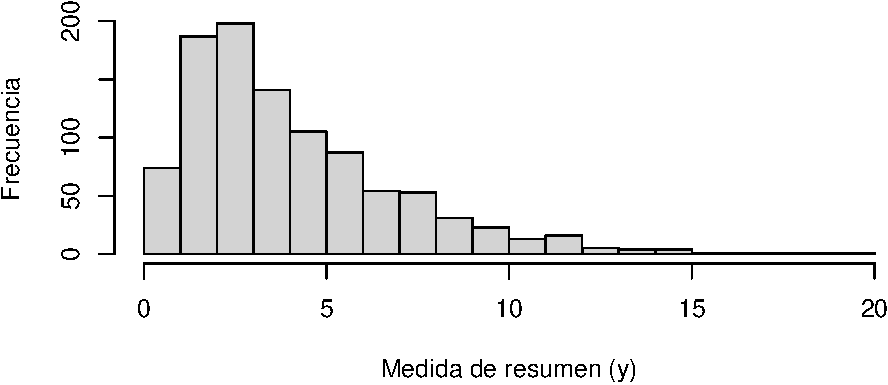
\includegraphics{04Estratificar_files/figure-latex/unnamed-chunk-1-1.pdf}
\caption{\label{fig:unnamed-chunk-1}\emph{Histograma de la medida de resumen (y) sobre las UPM}}
\end{figure}

Por ende, si esta característica es altamente sesgada, es recomendable crear un estrato de inclusión forzosa con estas unidades. Esta práctica asegura que el error de muestreo para este estrato sea nulo.

\hypertarget{particiuxf3n-en-cuantiles-q}{%
\subsection*{Partición en cuantiles (Q)}\label{particiuxf3n-en-cuantiles-q}}
\addcontentsline{toc}{subsection}{Partición en cuantiles (Q)}

Este método divide la población de UPM en grupos creados a partir de la división en intervalos regulares de la distribución de la medida de resumen. Los cuantiles más usados son los cuartiles (que dividen la población en cuatro grupos), los quintiles (que dividen la población en cinco grupos) y los deciles (que dividen la población en 10 grupos); sin embargo, con los propósitos de estratificación, también es útil considerar la partición en terciles (que dividen la población en tres grupos).

\hypertarget{muxe9todo-de-rauxedz-de-frecuencia-acumulada-dh}{%
\subsection*{Método de raíz de frecuencia acumulada (DH)}\label{muxe9todo-de-rauxedz-de-frecuencia-acumulada-dh}}
\addcontentsline{toc}{subsection}{Método de raíz de frecuencia acumulada (DH)}

\citet{Dalenius_Hodges_1959} propusieron esta técnica de estratificación basada en la acumulación de la raíz cuadrada de las frecuencias acumuladas de la medida de resumen sobre las UPM. Esta técnica es exacta y no requiere de algún procedimiento iterativo. La idea principal de esta técnica es encontrar grupos que minimicen la siguiente función:

\[
D = \sum_{h=1}^H W_h \sqrt{S^2_{y_{h}}}
\]

En donde \(W_h = N_h/N\) (\(h = 1, \ldots, H\)) es el tamaño relativo del estrato \(h\) y \(S^2_{y_{h}}\) es la varianza de la medida de resumen en el estrato \(h\).

\hypertarget{estratificaciuxf3n-uxf3ptima-lh}{%
\subsection*{Estratificación óptima (LH)}\label{estratificaciuxf3n-uxf3ptima-lh}}
\addcontentsline{toc}{subsection}{Estratificación óptima (LH)}

\citet{Lavallee_Hidiroglou_1988} propusieron por primera vez la construcción de una estratificación óptima para poblaciones de encuestas reales, basada en la minimización de una expresión ligada al tamaño de muestra. Más adelante \citet{Kozak_2004} definió un algoritmo iterativo mediante arranques aleatorios para optimizar el proceso de minimización.

\hypertarget{estratificaciuxf3n-geomuxe9trica-gh}{%
\subsection*{Estratificación geométrica (GH)}\label{estratificaciuxf3n-geomuxe9trica-gh}}
\addcontentsline{toc}{subsection}{Estratificación geométrica (GH)}

\citet{Gunning_Horgan_2004} desarrollaron este método con el objetivo de que los coeficientes de variación de la medida de resumen tiendan a ser iguales dentro de los estratos y, de esta forma, encontraron que los límites que definían estos grupos estaban conformados en progresión geométrica.

\hypertarget{metodologuxedas-multivariadas-sobre-la-matriz-de-informaciuxf3n}{%
\section{Metodologías multivariadas sobre la matriz de información}\label{metodologuxedas-multivariadas-sobre-la-matriz-de-informaciuxf3n}}

Partiendo de la matriz de información \(\mathbf{X}\) a nivel de las UPM, es posible considerar algunos procedimientos que no necesitan de la reducción a una sola dimensión, sino que admiten tantas dimensiones como indicadores definidos en las columnas de la matriz \(\mathbf{X}\). Teniendo en cuenta que en el periodo intercensal se realizarán encuestas que miden variables que están fuertemente ligadas a las observadas en el censo, entonces encontrar una estratificación que sea óptima para todo el conjunto de variables de la matriz de información asegurará una partición óptima para todas las encuestas realizadas en el periodo intercensal. Las siguientes metodologías permiten minimizar conjuntamente la varianza de los \(P\) estimadores de muestreo en un diseño estratificado.

\hypertarget{k-medias-de-jarque-kmj}{%
\subsection*{K-medias de Jarque (KmJ)}\label{k-medias-de-jarque-kmj}}
\addcontentsline{toc}{subsection}{K-medias de Jarque (KmJ)}

\citet{Jarque_1981} propone utilizar una versión modificada del algoritmo de K-medias \citep{Macqueen_1967}, cuya objetivo es la minimización de la siguiente función de distancia:

\[
\sum_{h=1}^H \sum_{k\in U_h}(\mathbf x_k - \bar {\mathbf x}_h)'\boldsymbol \Lambda^{-1}(\mathbf x_k - \bar {\mathbf x}_h)
\]

En donde \(\mathbf x_j\) corresponde a la medición de las \(P\) variables de la matriz de información en la \(k\)-ésima UPM, \(\bar {\mathbf x}_h\) es el vector de medias de la matriz de información en el estrato \(h\) y \(\boldsymbol \Lambda\) es una matriz diagonal de tamaño \(P \times P\) cuyas entradas se definen como la varianza de las \(P\) variables de la matriz \(\mathbf X\), es decir \(\boldsymbol \Lambda [p,p]=S^2_{x_p}\). Esta modificación tiene como objetivo minimizar la relación entre la varianza de un estimador de muestreo estratificado con asignación proporcional y la de un muestreo aleatorio simple. Como se puede ver en el anexo, cuando \(\boldsymbol \Lambda = \mathbf I\), el algoritmo resultante es idéntico al algoritmo clásico de K-medias.

\hypertarget{particiuxf3n-genuxe9tica-bb}{%
\subsection*{Partición genética (BB)}\label{particiuxf3n-genuxe9tica-bb}}
\addcontentsline{toc}{subsection}{Partición genética (BB)}

\citet{Ballin_Barcaroli_2013} argumentan que la mejor estratificación es aquella partición del marco de muestreo que asegura el mínimo costo muestral que satisfaga algunas restricciones de precisión; o, que maximice la precisión de los indicadores de interés bajo las restricciones. Haciendo uso de algoritmos genéticos evolutivos, esta la estratificación multivariada del marco de muestreo parte de la consideración de estratificaciones univariadas independientes (una para cada variable de la matriz de información) y de la definición del producto cartesiano resultante de todas estas particiones (estratos atómicos). Este universo de posibles estratificaciones evoluciona, sujeto a las restricciones de precisión sobre cada variable de la matriz de información, hasta converger en el número de estratos definidos de antemano \(H\).

\hypertarget{evaluaciuxf3n-y-escogencia-de-la-mejor-estratificaciuxf3n}{%
\section{Evaluación y escogencia de la mejor estratificación}\label{evaluaciuxf3n-y-escogencia-de-la-mejor-estratificaciuxf3n}}

En la evaluación de los escenarios de estratificación entran las técnicas univariadas y multivariadas. Al final, el resultado de aplicar una u otra técnica es simplemente una clasificación de las UPM. Por lo tanto, cada una de las posibles estratificaciones debe ser evaluada con base en la reducción de la varianza para todos los indicadores considerados en la matriz de clasificación. La medida clásica con la que se juzgan las bondades de una estrategia de muestreo es el efecto de diseño (DEFF). Por lo tanto, la evaluación de la estratificación debe estar supeditada también a esta medida, que para la variable \(p = 1, \ldots, P\), está dada por:

\[
DEFF_p = \frac{Var_{ST}(\bar x _p)}{Var_{SI}(\bar x _p)} \ \ \ \ \ \ \ \ \ p = 1, \ldots, P.
\]

En donde, \(Var_{ST}(\bar x _p)\) y \(Var_{SI}(\bar x _p)\) denotan la varianza del diseño estratificado y la varianza de un muestreo aleatorio simple para la media poblacional (porcentaje) de la \(p\)-ésima variable de la matriz de información. Por otro lado, \citet[página 184]{Gutierrez_2016} demuestra que, cuando la asignación es proporcional, esta relación se puede escribir de la siguiente manera:

\[
DEFF_p = \frac{ \sum_{h=1}^H W_h S^2_{x_{hp}} }{S^2_{x_p}} \ \ \ \ \ \ \ \ \ p = 1, \ldots, P.
\]

En donde, para cada estrato \(h = 1, \ldots, H\), se tiene que \(S^2_{x_p}\) es la varianza de la variable \(x_p\) en la población y \(S^2_{x_{hp}}\) es la varianza de la variable \(x_p\) supeditada al estrato \(h\). Nótese que una ventaja de expresar el efecto de diseño como en la ecuación anterior es que no dependerá del tamaño de muestra. Una vez definido el criterio de evaluación de la estratificación sobre una variable \(x_p\), es necesario definir un criterio de estratificación multivariante que contemple cada una de las \(P\) variables. Siguiendo las ideas de \citet{Jarque_1981}, se propone la siguiente medida de calidad, definida como el \emph{efecto de diseño generalizado} (\(G(S)\)) sobre todas las variables de la matriz de información:

\[
G(S) = \sum_{p=1}^P DEFF_p = \sum_{p=1}^P \frac{1}{S^2_{x_p}}\sum_{h=1}^H W_h S^2_{x_{hp}}
\]

Ante una estratificación pertinente, se esperaría que \(Var_{ST}(\bar x _p) < Var_{SI}(\bar x _p)\), por lo tanto \(0 < DEFF_p < 1\), lo que conlleva a que \(0 < F(S) < P\). Luego, se debería escoger el escenario para el cual \(F(S)\) fuera mínimo. Nótese que, para cada uno de los escenarios en estudio, es necesario fijar el número de estratos; en general se propende porque el número de grupos esté entre tres y cinco. Esta escogencia del número de grupos debe ser discutida al interior del INE con los equipos que determinan la rotación de las UPM en cada periodo de levantamiento de las encuestas de hogares. Escoger un número alto de estratos reducirá la varianza, pero a su vez puede tener repercusiones negativas en la logística de rotación del diseño de muestreo de las encuestas, haciendo que se agoten rápidamente las UPM dentro de los estratos geográficos y socioeconómicos. Por lo anterior, se recomienda restringir los escenarios de evaluación a la consideración de \(H=3\) y \(H=4\) estratos.

El siguiente cuadro ejemplifica la evaluación de estas técnicas para dos escenarios de estratificación (tres y cuatro estratos) en una matriz de información que contiene 8 variables. De la tabla se puede deducir varias conclusiones interesantes. Por ejemplo, para el primer indicador, la mejor estratificación es DH con cuatro estratos; para el segundo indicador, la mejor estratificación es BB con cuatro estratos; mientras que para el último indicador, la mejor estratificación es LH con cuatro estratos. Como se puede notar, para cada indicador existirá un método que induzca una mayor eficiencia, pero que para otros indicadores puede ser deficiente. Esto claramente muestra que la estratificación con respecto a un solo indicador puede ser un procedimiento inadecuado. Por lo tanto, basados en este ejemplo, el mejor método sería DH con cuatro estratos puesto que induce una mayor eficiencia conjunta al reducir el efecto de diseño generalizado.

\footnotesize

\begin{longtable}[]{@{}
  >{\raggedleft\arraybackslash}p{(\columnwidth - 24\tabcolsep) * \real{0.08}}
  >{\raggedleft\arraybackslash}p{(\columnwidth - 24\tabcolsep) * \real{0.07}}
  >{\raggedleft\arraybackslash}p{(\columnwidth - 24\tabcolsep) * \real{0.08}}
  >{\raggedleft\arraybackslash}p{(\columnwidth - 24\tabcolsep) * \real{0.08}}
  >{\raggedleft\arraybackslash}p{(\columnwidth - 24\tabcolsep) * \real{0.08}}
  >{\raggedleft\arraybackslash}p{(\columnwidth - 24\tabcolsep) * \real{0.08}}
  >{\raggedleft\arraybackslash}p{(\columnwidth - 24\tabcolsep) * \real{0.08}}
  >{\raggedleft\arraybackslash}p{(\columnwidth - 24\tabcolsep) * \real{0.07}}
  >{\raggedleft\arraybackslash}p{(\columnwidth - 24\tabcolsep) * \real{0.08}}
  >{\raggedleft\arraybackslash}p{(\columnwidth - 24\tabcolsep) * \real{0.08}}
  >{\raggedleft\arraybackslash}p{(\columnwidth - 24\tabcolsep) * \real{0.08}}
  >{\raggedleft\arraybackslash}p{(\columnwidth - 24\tabcolsep) * \real{0.08}}
  >{\raggedleft\arraybackslash}p{(\columnwidth - 24\tabcolsep) * \real{0.08}}@{}}
\caption{\emph{Efectos de diseño \(DEFF_p\) y efecto de diseño generalizado \(G(S)\) considerando tres (\(H=3\)) y cuatro (\(H=4\)) estratos para ocho variables.}}\tabularnewline
\toprule
DEFF & Q (H=3) & DH (H=3) & LH (H=3) & GH (H=3) & KmJ (H=3) & BB (H=3) & Q (H=4) & DH (H=4) & LH (H=4) & GH (H=4) & KmJ (H=4) & BB (H=4) \\
\midrule
\endfirsthead
\toprule
DEFF & Q (H=3) & DH (H=3) & LH (H=3) & GH (H=3) & KmJ (H=3) & BB (H=3) & Q (H=4) & DH (H=4) & LH (H=4) & GH (H=4) & KmJ (H=4) & BB (H=4) \\
\midrule
\endhead
\(\bar x_1\) & 0.87 & 0.85 & 0.81 & 0.82 & 1 & 0.88 & 0.8 & 0.70 & 0.76 & 0.72 & 0.71 & 0.77 \\
\(\bar x_2\) & 0.89 & 0.82 & 0.95 & 0.97 & 0.94 & 0.88 & 0.79 & 0.74 & 0.75 & 0.77 & 0.75 & 0.71 \\
\(\bar x_3\) & 0.87 & 0.97 & 0.83 & 0.96 & 0.89 & 0.95 & 0.74 & 0.75 & 0.79 & 0.7 & 0.79 & 0.71 \\
\(\bar x_4\) & 0.92 & 0.89 & 0.81 & 0.94 & 0.96 & 1 & 0.77 & 0.73 & 0.73 & 0.7 & 0.71 & 0.74 \\
\(\bar x_5\) & 0.85 & 0.83 & 0.96 & 0.96 & 0.83 & 0.81 & 0.8 & 0.73 & 0.8 & 0.78 & 0.8 & 0.79 \\
\(\bar x_6\) & 0.87 & 0.88 & 0.9 & 0.88 & 0.86 & 0.81 & 0.8 & 0.72 & 0.76 & 0.7 & 0.74 & 0.73 \\
\(\bar x_7\) & 0.87 & 0.95 & 0.99 & 0.83 & 0.86 & 0.84 & 0.75 & 0.7 & 0.77 & 0.72 & 0.77 & 0.77 \\
\(\bar x_8\) & 0.93 & 0.82 & 0.91 & 0.99 & 0.93 & 0.88 & 0.77 & 0.74 & 0.72 & 0.78 & 0.76 & 0.75 \\
G(S) & 7.07 & 7.01 & 7.16 & 7.35 & 7.27 & 7.05 & 6.22 & 5.81 & 6.08 & 5.87 & 6.03 & 5.97 \\
\bottomrule
\end{longtable}

\normalsize

Para tener comparabilidad y consistencia, los algoritmos de estratificación se deberían aplicar sobre cada una de las UPM en las áreas urbanas, pero independientemente de las UPM rurales. La escogencia del número de estratos debe ser discutida al interior de los INE y así determinar si escoger un número alto de estratos reduce la varianza significativamente, o si puede tener repercusiones negativas en la logística de rotación y desgaste de las UPM, haciendo que se agoten rápidamente dentro del cruce de los estratos geográficos y socioeconómicos. Es recomendable restringir los escenarios de evaluación a la consideración de H=3 o H=4 estratos. Este último componente es importante puesto que los diseños de muestreo deberían considerar un tamaño de muestra mínimo de dos UPM por estrato para poder estimar la varianza del estimador \citep{Gutierrez_2016}.

El efecto diseño no es el único aspecto por evaluar para la elección del procedimiento de estratificación. Es necesario verificar la estabilidad del método con respecto a los otros procedimientos de estratificación. Por ejemplo, la siguiente tabla muestra la matriz de coincidencias entre las diferentes clasificaciones de los estratos.

\begin{longtable}[]{@{}cccccccc@{}}
\toprule
Técnica & Jarque & K-means & DAL & GEO & LH-S & LH-K & Percentil \\
\midrule
\endhead
\textbf{Jarque} & 1 & 0,64 & 0,92 & 0,84 & 0,89 & 0,89 & 0,82 \\
\textbf{K-means} & 0,64 & 1 & 0,68 & 0,62 & 0,71 & 0,71 & 0,74 \\
\textbf{DAL} & 0,92 & 0,68 & 1 & 0,82 & 0,96 & 0,96 & 0,90 \\
\textbf{GEO} & 0,84 & 0,62 & 0,82 & 1 & 0,78 & 0,78 & 0,73 \\
\textbf{LH-S} & 0,89 & 0,71 & 0,96 & 0,78 & 1 & 1,00 & 0,93 \\
\textbf{LH-K} & 0,89 & 0,71 & 0,96 & 0,78 & 1,00 & 1 & 0,93 \\
\textbf{Percentil} & 0,82 & 0,74 & 0,90 & 0,73 & 0,93 & 0,93 & 1 \\
\bottomrule
\end{longtable}

Por último, suponiendo que se decidió la creación de tres estratos se encuentran numerado en orden ascendente que indica el nivel de bienestar socioeconómico, también se debe evaluar la coherencia de la distribución de las diferentes variables agregadas a nivel de UPM en los estratos. Por ejemplo, la proporción de personas mayores de 15 años alfabetizadas debería tener mayor incidencia en los estratos más altos, y este patrón también se debería observar para diferentes indicadores como la proporción de hogares con internet, la proporción de tenencia de refrigerador, la proporción de tenencia de televisión por cable, la proporción de tenencia de automovil, la proporción de hogares con saneamiento adecuado, la proporción de hogares con pisos adecuados, la proporción de personas con educación superior, entre otras. La figura \ref{fig:estrata} muestra el comportamiento esperado en los estratos de muestreo para algunas variables de interés. De esta forma, el estrato uno debería presentar condiciones económicas más adversas, el estrato dos debería tener mejores condiciones, siendo el tercer estrato el que agrupa a las UPM con menores dificultades socioeconómicas. En el área rural debiesen aparecer una menor proporción de UPM en el estrato 3, dadas las condiciones menos favorables.

\begin{figure}
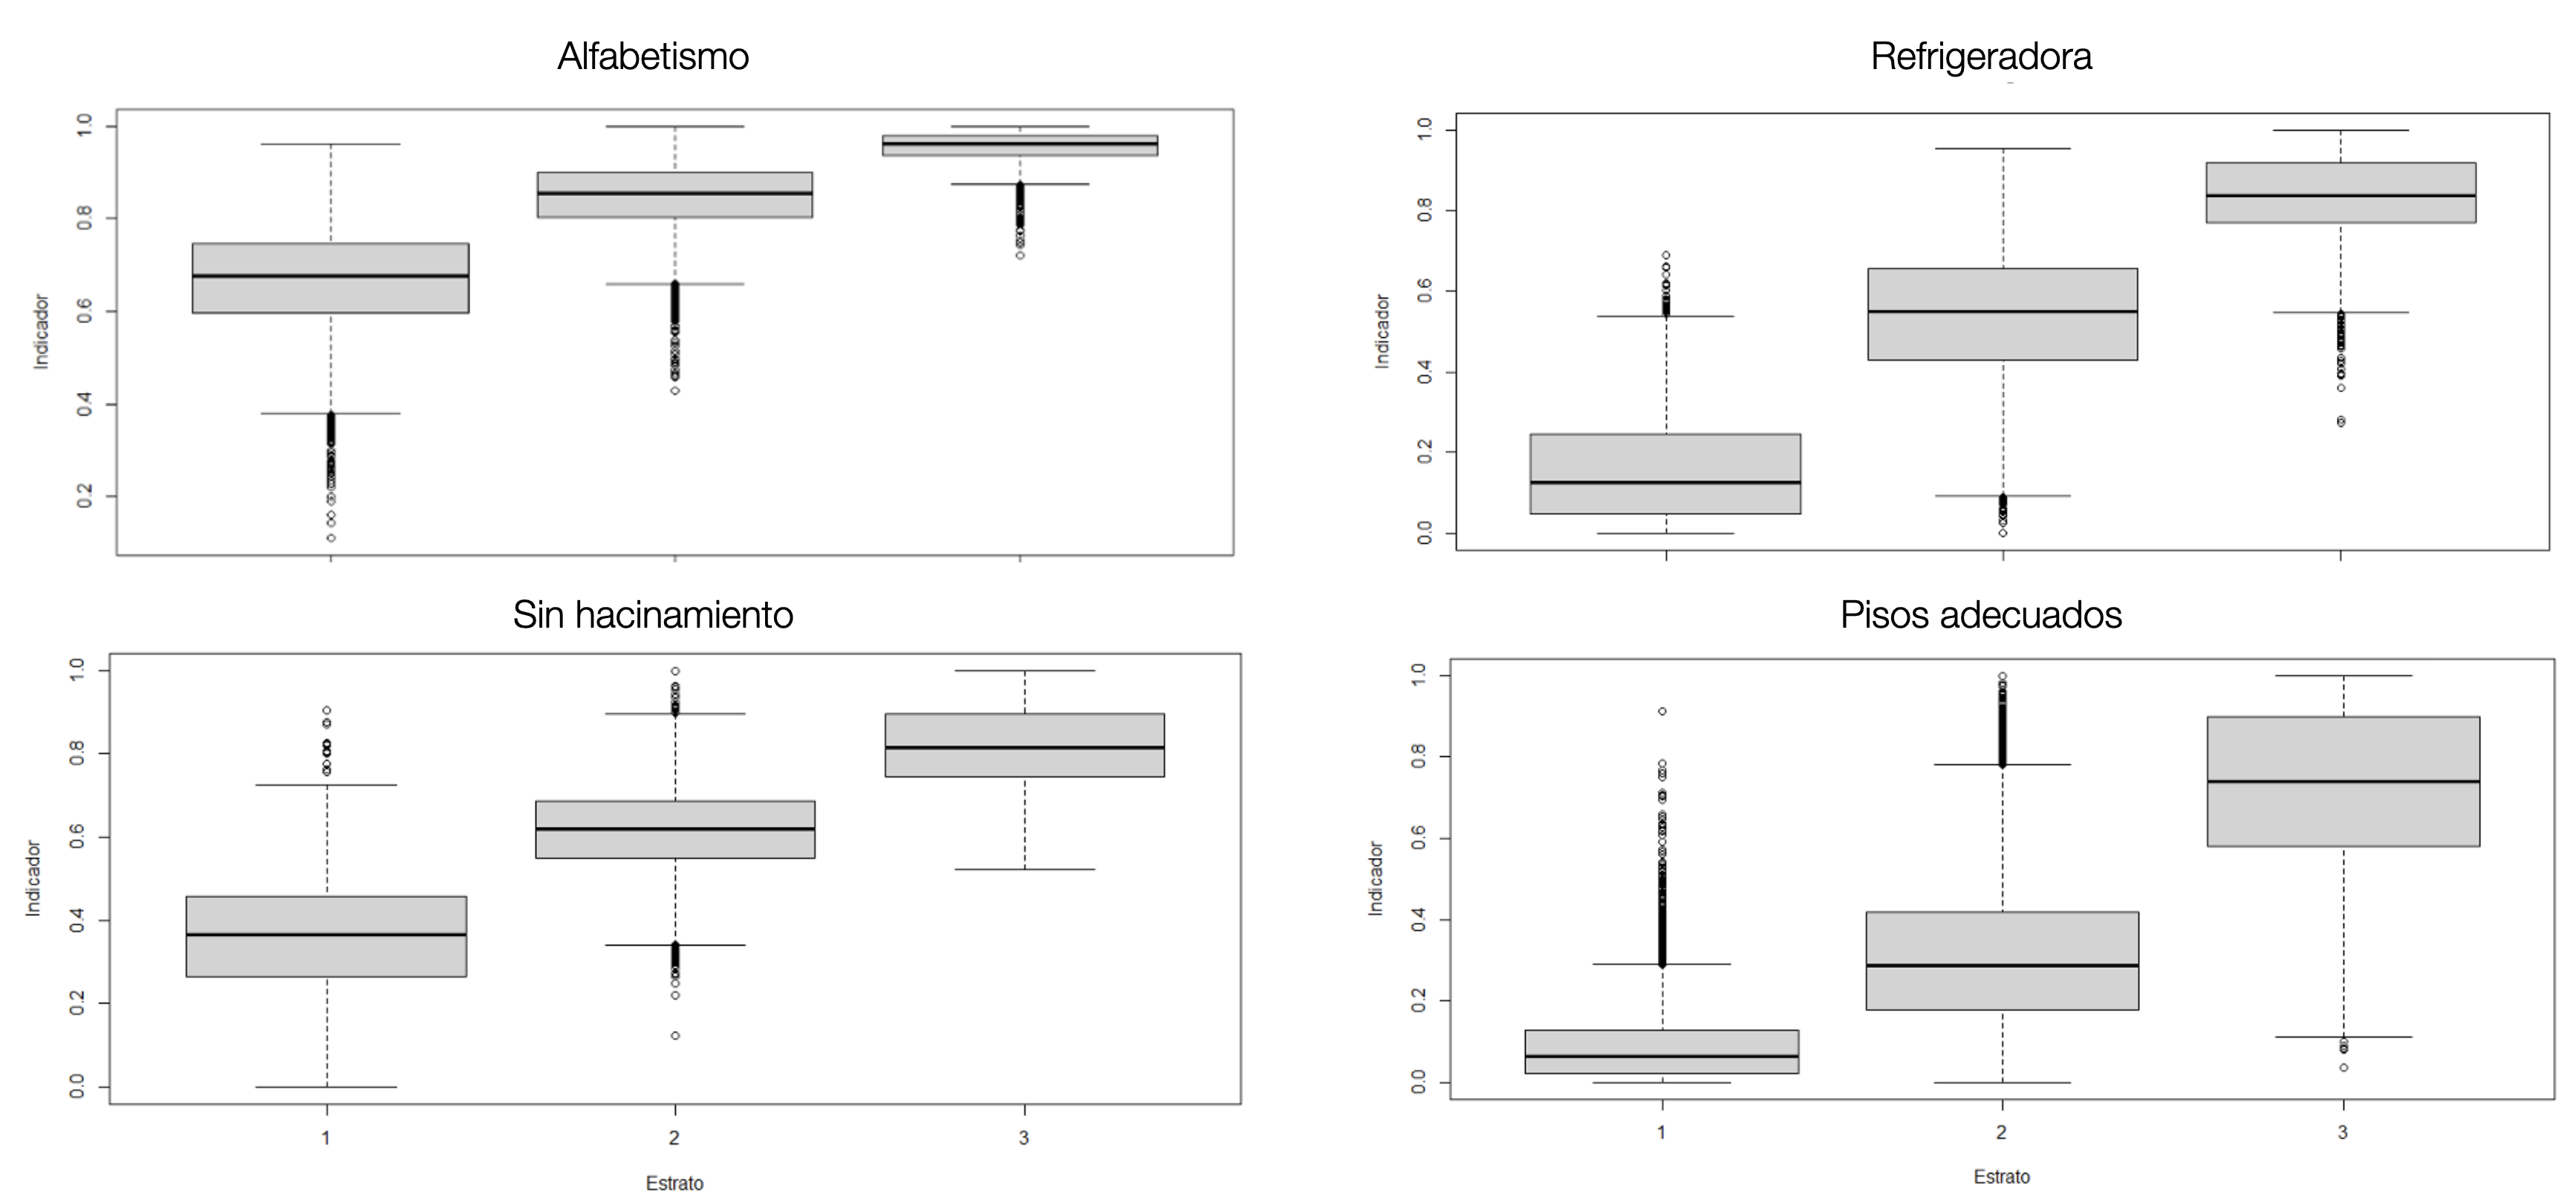
\includegraphics[width=800px]{Pics/Estratificar} \caption{Comportamiento esperado en los estratos de muestreo para algunas variables de interés.}\label{fig:estrata}
\end{figure}

Si la contribución de algunas unidades al total poblacional es no significativa, y además esas unidades son de difícil acceso, es común que en algunos países de la región se opte por redefinir el universo y crear un estrato de exclusión forzosa. En este estrato no se realiza ninguna encuesta y las respectivas estimaciones no tendrán en cuenta a esta población excluida. Por último, como algunos procedimientos de clasificación se basan en la generación de números aleatorios, se recomienda documentar los códigos computacionales que se utilizaron para que los resultados puedan ser replicados, por lo que debe fijar una semilla aleatoria al comienzo del código computacional.

\hypertarget{estratificaciuxf3n-impluxedcita}{%
\section{Estratificación implícita}\label{estratificaciuxf3n-impluxedcita}}

Los estratos explícitos definidos en la sección anterior son útiles para reducir la varianza de muestreo y asegurar la representatividad de la muestra en cada uno de los subgrupos que comparten las mismas características socioeconómicas, dentro de los mismos municipios. Además de los estratos socioeconómicos, algunas variables que se consideran en el proceso de estratificación explícita son:

\begin{itemize}
\tightlist
\item
  Estados o regiones de un país.
\item
  Zona en la que está ubicado el hogar: urbana o rural. Nótese que cada país brinda su definición de ruralidad, acorde a las definiciones nacionales.
\end{itemize}

También es posible realizar una selección ordenada que induce una estratificación implícita, sin que necesariamente se tenga control sobre el tamaño de muestra final, y sin asumir independencia en la selección. Este tipo de estratificación es una forma de garantizar una asignación estrictamente proporcional de los hogares en todos los estratos implícitos. También puede conducir a una mayor confiabilidad de las estimaciones de la encuesta, siempre que las variables de estratificación implícita que se consideren estén correlacionadas con los indicadores de interés (por ejemplo, la tasa de desocupación, subocpupación o informalidad).

La estratificación implícita es altamente recomendada cuando la encuesta está enfocada en un tema particular (como por ejemplo el mercado de trabajo) y requiere el uso del muestreo sistemático (con probabilidades simples o desiguales) en la selección de las UPM. Según \citet[pág. 46]{UN_2008}, en la mayoría de países la secuencia podría empezar con el área urbana, desagregada por departamento, a su vez desagregada por municipio; seguida del área rural, desagregada por departamento, a su vez desagregada por comuna o vereda. La selección sistemática de UPM deberá estar supeditada al ordenamiento de las UPM por el número de viviendas.

Nótese que la estratificación implícita puede constituir un método objetivo de selección de reemplazos de las UPM a laas cuales no se pudo acceder en el operativo de campo; de esta forma, si una UPM fue seleccionada originalmente, pero por alguna razón operativa no puede ser empadronada, su reemplazo será la inmediatamente anterior (o posterior) en la lista estratificada implícitamente. Nótese que este procedimiento ubicará el reemplazo como la UPM ubicada en el mismo municipio, dentro del mismo departamento, en la misma zona y con un número similar de viviendas.

Aunque la estratificación implícita permite acotar el sesgo generado por la ausencia de respuesta de las UPM, \citet[págs. 348 - 349]{Vehovar_1999} advierte que se debe tener precaución en cuanto a los usos de esta práctica puesto que puede conllevar sesgos importantes en las estimaciones de interés. Lo anterior se desprende del hecho de que los individuos ubicados en zonas donde sí es posible acceder diferirán significativamente de aquellos ubicados en las zonas de difícil acceso.

Por esta razón es útil que, después de haber valorado los posibles sesgos, si se ha tomado la determinación de realizar las sustituciones sobre las UPM de difícil acceso, se realice un seguimiento exhaustivo en cada levantamiento que permita clasificar el esquema de recolección de información primaria y se valore su impacto en la precisión de los estimadores resultantes.

\hypertarget{diseuxf1o-y-mecanismo-de-selecciuxf3n-de-la-muestra}{%
\chapter{Diseño y mecanismo de selección de la muestra}\label{diseuxf1o-y-mecanismo-de-selecciuxf3n-de-la-muestra}}

Todas las encuestas de hogares en la región comparten el mismo principio inferencial: la selección de una muestra que puede representar la población de todo un país. Por supuesto, ante este objetivo tan ambicioso, es necesario contar con procedimientos robustos, probados y capaces de pasar los filtros más críticos y agudos. Tal vez en este momento de la historia, la práctica de estos procedimientos ya no genere ningún tipo de asombro, pero el lector podría animarse a contemplar todas los posibles escenarios que una sociedad enfrentaría ante la ausencia de las encuestas de hogares y sus repercusiones en materia del desarrollo social.

Es innegable la potencia y el poder que hay detrás de estas operaciones estadísticas que están sustentadas en el muestreo probabilístico que induce una inferencia que procede de lo particular a lo general, puesto que al seleccionar una muestra, esta sirve como base para obtener conclusiones acerca de la población. Al final la muestra será un vehículo adecuado para representar las características más importantes de la población en estudio, en la forma en que justamente las variables se incorporan en el formulario de la encuesta. \citet{Gutierrez_2016} afirma que el muestreo es un procedimiento que responde a la necesidad de información estadística precisa sobre la población y los conjuntos de elementos que la conforman; el muestreo probabilístico trata con investigaciones parciales que apuntan a inferir a la población completa y en general está basado en los siguientes principios:

\begin{itemize}
\tightlist
\item
  \emph{Aleatorización}: las unidades incluidas en la muestra son seleccionadas mediante un proceso probabilístico. De esta forma, además de eliminar los posibles sesgos de selección, la muestra resultante será válida para cualquier proceso de inferencia, puesto que se basa en el conjunto de todas las muestras que se pueden obtener con el esquema de muestreo definido.
\item
  \emph{Inclusión}: todas las unidades de la población tienen una probabilidad no nula de ser incluidas en la muestra. Lo anterior quiere decir que el procedimiento de selección le da chance de ser seleccionado a todas las unidades que componen la población. De esta manera, la muestra final puede estar compuesta por cualquier combinación plausible de hogares o individuos.
\end{itemize}

Para que los anteriores principios se cumplan a cabalidad, es necesario contar con un instrumento que permita seleccionar a los hogares del país de forma exhaustiva y completa; esto quiere decir que el instrumento debería contener todos y cada uno de los hogares de la población. Dado que no existe una lista que permita identificar y ubicar a cada uno de los hogares de la población, entonces se deben contemplar otras posibilidades que permitan lograr el objetivo. Debido al principio natural de la aglomeración de las poblaciones humanas, es posible lograr este cometido de manera indirecta a través de la definición de los marcos de muestreo de áreas.

Las encuestas han tenido una gran trascendencia en la evolución de las mediciones de los indicadores sociales, que a su vez conllevan a que los gobiernos realicen un seguimiento y monitoreo de las cifras más importantes para la sociedad. De esta forma se podrá investigar la efectividad de las políticas públicas, para concretar las metas de mejora en las condiciones sociales y/o económicas de la ciudadanía. Tal como lo afirma \citet{Gutierrez_2016}, el muestreo es un procedimiento que responde a la necesidad de información estadística precisa sobre la población y los conjuntos de elementos que la conforman. De esta forma, una muestra bien seleccionada de unos cuantos miles de individuos puede representar con gran precisión a una población de millones de personas.

En general, se puede afirmar que un concepto apropiado por la sociedad es el que define a una muestra representativa como un modelo reducido de la población. De este concepto se desprende un argumento de validez sobre la muestra: ``una buena muestra es aquella que se parece a la población, de tal forma que las categorías aparecen con las mismas proporciones que en la población''. Sin embargo, en algunos casos es fundamental ``sobrerepresentar'' algunas categorías o incluso seleccionar unidades con probabilidades desiguales \citep{Tille2006}. La muestra no debe ser un modelo reducido de la población; debe ser una herramienta usada para obtener estimaciones válidas: exactas, confiables, precisas y consistentes.

El concepto de muestra representativa no se debe usar para referirse a que la muestra debe parecerse a la población. La teoría de muestreo se ha ocupado de estudiar estrategias óptimas que permitan asegurar la calidad de las estimaciones; en general, el concepto de representatividad debe estar asociado con la estrategia de muestreo y no sólo con las muestra seleccionada. Consecuentemente, la muestra como subconjunto de la población es una herramienta que no admite el calificativo de representativa, puesto que su objetivo no es parecerse a la población sino permitir que, mediante la correcta caracterización de una estrategia de muestreo, el proceso de inferencia logre reproducir la estructura de la población.

Lo anterior no indica que debamos abandonar del todo este adjetivo (representativo) en los proceso de muestreo. Por el contrario, el objetivo del equipo técnico experto en la selección de muestras debe estar supeditado a lograr que efectivamente este adjetivo se pueda aplicar a todo el componente de diseño y estimación. Es decir, el calificativo de representatividad es objeto de un proceso conjunto de diseño de muestreo, estimación de parámetros, acercamiento a modelos estadísticos para hacer frente a la ausencia de respuesta, entre otros. Uno de los objetivos de este capitulo será hacer precisión sobre las estructuras de selección de las muestras en las encuestas por muestreo. Al escoger un mecanismo apropiado para la selección de la muestra, será posible afirmar que la estrategia de muestreo es efectivamente representativa de la población de interés, puesto que cumple con altos estándares de rigurosidad y calidad en cada uno de los componentes del proceso.

\hypertarget{diseuxf1os-de-muestreo}{%
\section{Diseños de muestreo}\label{diseuxf1os-de-muestreo}}

Una vez que los marcos de muestreo se han refinado y se ha definido una estratificación apropiada para las UPM que las componen, es necesario realizar el proceso de muestreo la selección final de los hogares. Este proceso de selección debe inducir insesgamiento, además de ser eficiente. Esto quiere decir que la inclusión de las unidades en la muestra estará supeditada a un esquema probabilístico libre de cualquier sesgo. Además de esto, se necesita que este mecanismo genere la menor dispersión posible en el proceso inferencial posterior.

El procedimiento de muestreo le asigna una probabilidad de selección conocida a cada posible muestra. Al diseñar un muestreo probabilístico, el investigador es el encargado de asignar estas probabilidades, mediante la definición del diseño de muestreo \citep{Sarndal_Swensson_Wretman_2003}. Aunque esta asignación de probabilidades se realiza de manera teórica, la pericia del equipo técnico deberá establecer cuál es la mejor forma de selección, y sobre esta escoger el mejor algoritmo de muestreo. Luego de establecer este conjunto de probabilidades, una única muestra es escogida mediante un mecanismo aleatorio que siga a cabalidad esta configuración estocástica inducida por el diseño de muestreo. Las probabilidades deben ser distintas de cero puesto que, de lo contrario, no se podría garantizar una inferencia insesgada, puesto que estaría excluyendo algunos sectores cartográficos del país. Además, estas mismas probabilidades se utilizan para crear los factores de expansión que definen todo el proceso de estimación, junto con el cálculo de los errores de muestreo, como se verá en los capítulos posteriores.

Existe una clara diferenciación entre un diseño de muestreo y un algoritmo de muestreo. El primero indica qué probabilidad de selección tendrán las posibles muestras en el soporte de muestreo, definido como el conjunto de todas las posibles muestras. Y el último se define como el proceso de selección de una única muestra que respeta las probabilidades del diseño de muestreo. En la definición de una encuesta de hogares es indispensable que se establezcan de antemano estos dos componentes. Es decir, si se ha decidido que el diseño de muestreo sea en etapas, el equipo técnico deberá documentar exhaustivamente cada etapa de muestreo, definiendo sus correspondientes unidades de muestreo y por consiguiente, los diseños de muestreos en cada etapa. Luego, es igual de importante explicar qué algoritmos de selección serán utilizados en cada etapa de muestreo. De esta forma habrá total transparencia en la selección de las unidades y esto redunda en la obtención de cifras oficiales confiables y precisas.

Existen muchas formas de seleccionar una muestra de hogares y cada una de ellas induce una medida de probabilidad sobre los elementos que conforman la población de interés. En general, asociado a cada esquema particular de muestreo se define una única función que asocia a cada hogar \(k\) con una probabilidad de inclusión en la muestra \(s\), definida de la siguiente manera:

\[\pi_k = Pr (k \in s)\]

Estas probabilidades de inclusión de los hogares, inducidas por los diseños de muestreo asociados a cada encuesta, cumplen con las siguientes propiedades

\begin{enumerate}
\def\labelenumi{\arabic{enumi}.}
\tightlist
\item
  \(\pi_k > 0\)
\item
  \(\sum_U \pi_k = n\)
\end{enumerate}

Observe que la primera propiedad garantiza que ningún hogar será excluido de la selección inicial. Si bien no todos lo hogares serán seleccionados para pertenecer a la muestra \(s\), todos tendrán un chance de ser escogidos por el mecanismo de selección aleatoria. En segunda medida, el tamaño de la muestra de hogares estará inducido por la magnitud de las probabilidades de inclusión. Por esta razón, una encuesta con una tamaño de muestra grande asignará una mayor probabilidad de inclusión a todos los hogares, que una encuesta de tamaño de muestra más modesto. A continuación se presenta una lista no exhaustiva de diseños de muestreo utilizados en encuestas de hogares para la publicación de estadísticas oficiales, junto con la forma particular que toman las probabilidades de inclusión en cada esquema.

\hypertarget{muestreo-aleatorio-simple}{%
\subsection*{Muestreo aleatorio simple}\label{muestreo-aleatorio-simple}}
\addcontentsline{toc}{subsection}{Muestreo aleatorio simple}

Este diseño de muestreo supone que es posible realizar una enumeración de todas las posibles muestras de tamaño fijo y escoger una de ellas mediante una selección aleatoria que asigne la misma probabilidad a cada una. Para ejecutar este diseño de muestreo es necesario tener información suficiente y exhaustiva de la ubicación e identificación de todas las unidades de interés. Su uso es común en las etapas finales de selección de las encuestas, en donde los hogares o personas se seleccionan con las misma probabilidad. Por ejemplo, una vez se ha escogido un área de muestreo, una parte del operativo de campo deberá estar dedicada al enlistamiento de todas las viviendas en esa área seleccionada. Cuando se haya realizado este empadronamiento será posible asignarle la misma probabilidad de inclusión a cada vivienda en el área o en la UPM. Por ende, las probabilidades de inclusión en el muestreo aleatorio simple sin reemplazo son todas iguales y dadas por la siguiente expresión:

\[\pi_k = Pr(k \in s) =  \frac{\binom{1}{1}\binom{N-1}{n-1}}{\binom{N}{k}} = \frac{n}{N}\]

Como se verá en los siguientes capítulos, cuando se usa el estimador de Horvitz-Thompson en este diseño de muestreo para estimar un total poblacional, y suponiendo que \(S^2_{y_U}\) denota la varianza de la característica de interés en la población finita, entonces las expresiones del estimador puntual y su varianza, respectivamente, toman la siguiente forma:

\begin{align*}
\hat{t}_{y,\pi} &= \sum_{s} \frac{y_k}{\pi_k} \\
Var(\hat{t}_{y,\pi}) &= \frac{N^2}{n}\left(1-\frac{n}{N}\right)S^2_{y_U}
\end{align*}

Una variante de este tipo de esquemas de selección de muestras de hogares dentro de la UPM es el muestreo sistemático, en donde se ordena el marco con algún patrón predefinido y posteriormente se selecciona un primer hogar (como arranque aleatorio). A partir de ese primer hogar seleccionado, se incluyen los restantes hogares en la muestra mediante saltos sistemáticos equi-espaciados por el siguiente factor \(a = N/n\), conocido como el intervalo de salto. Por ejemplo, una muestra sistemática podría ser:
\[s=\{2, 12, 22, 32, 42\}\].

En donde el primer hogar elegido en la UPM fue el segundo y con saltos sistemáticos de diez hogares se va encuestando los restantes hogares en la lista. En este diseño la probabilidad de inclusión también es uniforme para cada hogar en la UPM y está dada por la siguiente expresión
\[\pi_k = Pr(k \in s) = \frac{1}{a} \approx \frac{n}{N}\]

\hypertarget{muestreo-proporcional-al-tamauxf1o}{%
\subsection*{Muestreo proporcional al tamaño}\label{muestreo-proporcional-al-tamauxf1o}}
\addcontentsline{toc}{subsection}{Muestreo proporcional al tamaño}

Este tipo de muestreo utiliza como insumo una característica de información auxiliar cuantitativa, también conocida como medida de tamaño (\emph{MOS}, por sus siglas en inglés). Para la ejecución de este diseño, necesariamente el marco de muestreo deberá contener el valor correspondiente a la medida de tamaño para cada una de sus unidades. Este muestreo es utilizado con frecuencia en las etapas iniciales de selección de las muestras, particularmente en la selección de las UPM que harán parte de la muestra. De esta forma, los conglomerados o UPM con más hogares o personas (medida de tamaño) tendrán una mayor probabilidad de ser seleccionados en la muestra. Por consiguiente, las probabilidades de inclusión en la muestra para las UPM serán desiguales y proporcionales a la medida de tamaño. Observe que la cantidad de individuos en las UPM es una cifra conocida, puesto que son resultado directo de los censos de población y vivienda.

Una de las ventajas de este tipo de muestreos es que hace más eficiente la estimación de los indicadores de interés. Para que esto ocurra, la medida de tamaño debe estar linealmente relacionada con la característica de interés. Esto a menudo sucede en las problemáticas sociales indagadas en las encuestas de hogares; puesto que a mayor número de hogares, se observa una mayor incidencia de estos fenómenos. Por ejemplo, restringidos a un estrato particular, es evidente que en las UPM con mas hogares se observarán mayor número de personas pobres, o de hogares con ingresos bajos, o de personas desocupadas, etc.

Por último, la medida de tamaño no necesariamente tiene que estar definida como el conteo simple de hogares o personas dentro de las UPM, también puede definirse como una función de estos conteos; por ejemplo, la raíz cuadrada, o incluso como una función compuesta de conteos de subpoblaciones. En el caso más simple, si \(N_i\) es la medida de tamaño de la \(i\)-ésima UPM \(U_i\), es decir el número de hogares que componen esa UPM; \(n_I\) el número de UPM que serán seleccionadas en cada estrato y \(N\) la sumatoria (o total) del número de hogares en todas las UPM del estrato (es decir, el número de hogares en el estrato) se tiene que las probabilidades de inclusión a la muestra \(s_I\) están dadas por la siguiente expresión:

\[\pi_i = Pr(U_i \in s_I) = n_I * \frac{N_i}{N}\]

Por último, no es cierto que la asignación de probabilidades desiguales en las unidades de muestreo induzca sesgo en la encuesta. Esta frase es cierta, siempre y cuando el estimador que se utilice no sea el adecuado. Por ejemplo, la frase pierde su validez cuando se utiliza el estimador de expansión (Hansen-Hurwitz, para el caso de muestreos con reemplazo - Horvitz-Thompson, en muestreos sin reemplazo). Ahora, lo natural es que si el diseño es con probabilidades desiguales, éstas se utilicen dentro de un estimador que considere esta desigualdad y lo menos usual es que se utilice el estimador de expansión en donde habría que corregir el sesgo causado por la omisión de las probabilidades desiguales.

\hypertarget{muestreo-estratificado}{%
\subsection*{Muestreo estratificado}\label{muestreo-estratificado}}
\addcontentsline{toc}{subsection}{Muestreo estratificado}

Esta familia de diseños de muestreo permite realizar inferencias precisas en subgrupos poblacionales de interés, usualmente definidos como agregaciones geográficas grandes. Por ejemplo, si se quieren estimaciones de la incidencia de la pobreza en las regiones geográficas de un país específico, entonces es pertinente que esta división geográfica sea considerada para la definición de los estratos. Como se mencionó al inicio de este capítulo, estas divisiones territoriales se forman de manera natural, puesto que los estratos ya están definidos como regiones de interés en el seguimiento de los indicadores sociales.

Una consecuencia directa de la estratificación es que cada subgrupo tendrá un marco de muestreo de UPM independiente, disyunto y mutuamente excluyente. Esta última caracterización induce una de las mayores ventajas del muestreo estratificado puesto que hay independencia entre los estratos. Esto significa que, al interior de cada estrato, se pueden ejecutar distintas estrategias de muestreo de forma independiente. Es común que en los países de América Latina el cruce de las áreas geográficas grandes junto con la división socioeconómica conformen los estratos (justo como se ilustró en los capítulos anteriores); asimismo una desagregación común en investigación social es la división territorial del país: urbano y rural. Evidentemente, la realidad social del entorno urbano difiere tanto del entorno rural que bien vale la pena considerar esta escisión en el diseño de muestreo de las encuestas de hogares.

Las probabilidades de inclusión definidas por este diseño de muestreo variarán en función de cada estrato. Por ejemplo, si en cada estrato (\(h=1, \ldots, H\)) se hubiese planeado un diseño aleatorio simple, entonces las probabilidades de inclusión estarían dadas por la siguiente expresión

\[\pi_k = Pr(k \in s_h) = \frac{n_h}{N_h}\]

Por supuesto, es posible que la estrategia de muestreo cambie dependiendo de los estratos. Por ejemplo, en la planificación de las encuestas de uso de tiempo, una de las características de interés por las cuales se quiere indagar es la cantidad de horas que hombres y mujeres dedican a actividades de trabajo no remuneradas. Esta realidad cambia radicalmente entre zonas rurales y urbanas. Para este tipo de encuestas de hogares, la flexibilidad que tienen los diseños estratificados es un baluarte valioso que permite definir estrategias de muestreo más precisas.

En algunas ocasiones, se ha sugerido que el muestreo estratificado es el mejor diseño para una encuesta de hogares, lo cual es parcialmente cierto. Aunque en muchas ocasiones, la opción de estratificar es adecuada e inclusive conveniente, no es cierto estrictamente que el muestreo estratificado sea el mejor diseño de muestreo. De hecho, la varianza inducida por el diseño aleatorio estratificado puede llegar a ser más grande cuando no hay una clara homogeneidad en el comportamiento de la característica de interés dentro de los estratos.

\hypertarget{muestreo-de-conglomerados}{%
\subsection*{Muestreo de conglomerados}\label{muestreo-de-conglomerados}}
\addcontentsline{toc}{subsection}{Muestreo de conglomerados}

Este diseño de muestreo surge como contraparte a la imposibilidad de generar una muestra de hogares directamente de un marco de muestreo que enliste todos y cada uno de los hogares en un país. De hecho, de forma hipotética, si fuese posible, los costos generados por una muestra aleatoria simple serían tan altos que la harían inviable desde el punto de vista presupuestario. Así, ante la ausencia de un marco de muestreo de las unidades de interés, y aprovechando el principio de aglomeración de las poblaciones humanas (que forman hogares y se aglomeran en segmentos, ciudades, regiones, etc.), la idea general detrás de este diseño es la conformación de unidades homogéneas entre sí (conglomerados), de las cuales se extraerá una muestra y para cada elemento del conglomerado se realizará un proceso exhaustivo de medición censal. De esta forma, es natural definir a las UPM como los conglomerados. Luego de seleccionar una muestra de estas UPM se realiza un censo de hogares sobre cada una de las UPM seleccionadas. Nótese que este proceso logístico induce un esquema con ventajas económicas en términos presupuestales, puesto que limita el operativo de campo a un cierto número de UPM que se deben medir exhaustivamente.

A pesar de que esta estrategia resulte conveniente desde el punto de vista logístico y operativo, ciertamente no lo es desde el punto de vista de la eficiencia estadística; los errores de muestreo que se producen al utilizar esta metodología son bastante más elevados que en un diseño simple, puesto que al realizar el proceso de aglomeración, generalmente la variación interna de los conglomerados es muy baja y la variación entre conglomerados tiende a ser muy alta, generando mayor incertidumbre en la inferencia de la encuesta. Para superar estos inconvenientes, se podría pensar en un esquema de muestreo que aumente el tamaño de la muestra de conglomerados; sin embargo, este aumento puede llegar a ser tan grande que, en algunos estratos, se deberían seleccionar todas las UPM. Por supuesto, se trata de un esquema inviable en la práctica, pero que da paso al esquema de muestreo más común en las encuestas de hogares: la selección por etapas.

Como se mencionó en los capítulos anteriores, definir los conglomerados con tamaños muy desiguales redunda en un aumento signigicativo de la varianza del estimador; es por esto que, en encuestas de hogares, se intenta crear conglomerados acotados, a nivel de manzana, o vereda. Esta es una práctica muy pertinente, puesto que la varianza del estimador de expansión estará en función de la varianza de los totales de los conglomerados; si existe una alta variación en los tamaños, habrá también una alta variación en los totales y, por consiguiente, la varianza del estimador será alta. De otra forma, si se tiene conocimiento de una característica de información auxiliar a nivel de los conglomerados (medida de tamaño), es posible hacer uso de esta información del marco para reducir la varianza en el estimador.

\hypertarget{muestreo-en-varias-etapas}{%
\subsection*{Muestreo en varias etapas}\label{muestreo-en-varias-etapas}}
\addcontentsline{toc}{subsection}{Muestreo en varias etapas}

En este esquema de muestreo, la idea general es retomar los principios del muestreo de conglomerados y realizar un submuestreo de hogares dentro de los conglomerados o UPM seleccionadas inicialmente. Este submuestreo puede ser tan incluyente como sea necesario. En general, en América Latina son muy comunes los esquemas de selección en dos etapas: en la primera etapa se selecciona una muestra de UPM y en la segunda etapa se selecciona una muestra de hogares en aquellas UPM seleccionadas en la primera etapa. Aunque, también es posible encontrar en algunos países esquemas en más de dos etapas. Por ejemplo, en una primera etapa se seleccionan municipios; en una segunda etapa se seleccionan UPM dentro de los municipios seleccionados; y en la segunda etapa se selecciona una muestra de hogares en aquellas UPM seleccionadas en la segunda etapa. Si un municipio es incluido en la muestra es posible realizar un proceso de aglomeración continúa sistemática, hasta llegar a la unidad de observación. Por ejemplo, en una ciudad seleccionada, es posible hacer un submuestreo de sus secciones cartográficas, luego seleccionar sectores cartográficos (contenidos en las secciones) y por último seleccionar hogares o personas.

Si el esquema de muestreo incluye la selección de municipios en la primera etapa, el diseño de muestreo apropiado en esta instancia deberá ser proporcional a una medida de tamaño, que puede ser definida como el número de habitantes de los municipios. De esta forma, con una probabilidad muy grande, a veces igual a uno, las ciudades más importantes (con más habitantes) serán siempre parte del estudio. Por otro lado, es posible que en algunas encuestas exista un submuetreo de personas dentro del hogar. En este caso, \citet{Clark_Steel_2007} aclaran que la escogencia de las personas dentro de los hogares no debería ser aleatoria simple puesto que ciertos grupos poblacionales podrían estar sub-representados o sobre-presentados. En general, el muestreo en varias etapas tiene dos características esenciales que lo hacen robusto, en términos estadísticos, y eficiente al momento de planear la logística del levantamiento de información; estas son:

\begin{itemize}
\tightlist
\item
  La independencia: que implica que no hay ninguna correlación en el diseño de muestreo de las unidades primarias de muestreo. Esto quiere decir que en cada UPM se puede ejecutar con independencia cualquier estrategia de muestreo que se crea apropiada para seleccionar la submuestra de hogares.
\item
  La invarianza: que implica que sin importar qué diseño de muestreo se ejecutó en la primera etapa para seleccionar las UPM, la segunda etapa de selección podrá ejecutarse de manera independiente de la primera etapa. Es decir, el submuestreo de los hogares es independiente del muestreo de las UPM.
\end{itemize}

Un esquema de selección bastante usado en las encuestas de hogares de América Latina es el relacionado con los diseños auto-ponderados, lo cuales, en la primera etapa de muestreo seleccionan \(n_I\) UPM con probabilidad proporcional al número de hogares que la habitan; es decir:

\[\pi_i = Pr(U_i \in S_i) = n_I \frac{N_i}{N}\]

En la segunda etapa de muestreo se seleccionan hogares dentro de las UPM que fueron incluidas en la etapa anterior. Esta selección de hogares se hace mediante un muestreo aleatorio simple, pero el tamaño de la submuestra es fijo para cada UPM. Es decir, no importa si una UPM es mucho más grande o más pequeña que las otras, el número de hogares que serán seleccionados será siempre el mismo. Por ejemplo, se podrían seleccionar \(n_0 = 10\) hogares por UPM, siempre. De esta forma, en la segunda etapa, la probabilidad de que el \(k\)-ésimo hogar sea seleccionado en la submuestra \(s_i\) de la UPM \(U_i\) que fue seleccionada en la muestra de la primera etapa \(s_I\), está dada por la siguiente expresión:

\[\pi_{k|i} = Pr(k \in s_i | U_i \in s_I ) = \frac{n_0}{N_i}\]

En los esquemas auto-ponderados, a pesar de tener dos diseños de muestreo diferentes en dos etapas (proporcional al tamaño y aleatorio simple), la probabilidad de inclusión de los hogares es siempre la misma para todos los hogares, como se puede ver en la siguiente expresión:

\[\pi_k = \pi_{k|i} * \pi_i = \frac{n_0}{N_i} \frac{n_I* N_i}{N} = \frac{n_0*n_I}{N} = \frac{n}{N}\]

Nótese que \(n = n_0 * n_I\) corresponderá con el número total de hogares que serán seleccionados, puesto que resulta ser la multiplicación del número de UPM que fueron seleccionadas en la primera etapa por el número de hogares que serán submuestreados en cada UPM en la segunda etapa. Este tipo de esquemas se utiliza cuando se quiere controlar el trabajo de campo y las cuotas por ciudad o municipio. Por otro lado, una particularidad de las encuestas de hogares es que, casi siempre, las personas y los hogares comparten las mismas probabilidades de inclusión. La razón de esto es que, en la mayoría de encuestas, el submuestreo de las personas es exhaustivo (censo en el hogar) y por ende, la probabilidad de inclusión en el submuestreo es forzosa.
\[\pi_k^{per} = Pr(persona \in hogar) =  1\]

Por lo anterior, se tiene que la probabilidad de inclusión de las personas en la muestra es idéntica a la del hogar:

\[1 * \pi_{k|i} * \pi_i = 1 * \frac{n}{N} = \frac{n}{N}\]

\hypertarget{muestreo-en-dos-fases}{%
\subsection*{Muestreo en dos fases}\label{muestreo-en-dos-fases}}
\addcontentsline{toc}{subsection}{Muestreo en dos fases}

En algunos casos en donde el marco de muestreo contiene poca o limitada información para proponer un diseño de muestreo eficiente, el investigador puede obtener información acerca de la población para construir un nuevo marco de muestreo reducido. En la primera fase, se selecciona una muestra de tamaño grande, conocida como \emph{muestra maestra}. Para cada uno de los elementos en esa muestra se debe obtener información sobre una o más variables auxiliares, con el fin de estratificar de mejor manera, recolectar información auxiliar en la muestra, o simplemente para obtener muestras sucesivas y comparables a lo largo del ciclo de vida de la encuesta. En la segunda fase, con la ayuda de la información obtenida en la primera fase, se selecciona una submuestra mediante un diseño de muestreo conveniente, mucho más eficiente y apropiado para estimar el fenómeno en estudio.

Por ejemplo, si se requieren estimativos precisos para distintos subgrupos poblacionales, pero no existe un marco de muestreo confiable o actualizado, que permita diseñar un muestreo estratificado, entonces es necesario realizar un esquema de muestreo en dos fases. De esta forma, se selecciona uma muestra aleatoria simple de tamaño moderado. Luego, se realiza un empadronamiento de los individuos en la muestra, a los cuales se eles pregunta acerca de su memebresía a los subgrupos poblacionales de interés. Luego, en una segunda fase, con ayuda de la información recolectada en la primera fase, se realiza un diseño estratificado.

Un ejemplo de este tipo de diseños de muestreo se da en el caso de México, en donde el INEGI ha planteado la construcción de una muestra maestra que permita seleccionar submuestras para las encuestas de hogares más importantes a la vez que se va recopilando información de los hogares pertenecientes a esta muestra maestra. En \citet{INEGI_MX_2012}, se menciona que \textless\textless a partir de la construcción del Marco Maestro de Muestreo 2012, se diseñó la Muestra Maestra para lograr mantener actualizada de forma continua la información de las viviendas particulares dentro de esta muestra. El diseño de la muestra maestra consideró y respetó las UPM formadas y la estratificación con que fue construido el marco de muestreo por lo que heredó la mayoría de sus propiedades. El diseño de la Muestra Maestra está basado en la cobertura, tamaño y distribución de las encuestas continuas y periódicas del INEGI. Los tamaños de muestra en viviendas para estas encuestas junto con el promedio óptimo de viviendas a seleccionar dentro de una UPM determinaron el número de UPM a seleccionar para la Muestra Maestra 2012\textgreater\textgreater. De esta forma, la muestra maestra constituye un elemento esencial para el levantamiento de la Encuesta Nacional de Ocupación y Empleo, la Encuesta Nacional sobre la Confianza del Consumidor, la Encuesta Nacional de Victimización y Percepción sobre Seguridad Pública, la Encuesta Nacional de Gasto de los Hogares, entre algunas otras.

En el caso de Costa Rica, la muestra de la Encuesta Nacional de Microempresas de los Hogares sigue un diseño en dos fases. La primera fase toma como base la Encuesta Nacional de hogares, en la cual se identifican aquellos hogares cuyos integrantes desarrollan actividades económicas concernientes con emprendimientos y microempresas. A partir de este listado exhaustivo, en una segunda fase, se selecciona a todas las personas al frente de estas microempresas y se les aplica un cuestionario con el fin de obtener información sobre sus características y sus actividades económicas. Por otro lado, en Chile se realiza el Estudio Nacional de la Discapacidad que asume un marco de muestreo reducido, en una primera fase, basado en la encuesta de hogares CASEN, en la cual se identifican los hogares que tienen miembros con alguna condición de discapacidad. En una segunda fase, se realiza una selección de hogares y mediante un cuestionario estructurado se indagan las características de las personas con esta condición.

\hypertarget{muestreo-balanceado}{%
\subsection*{Muestreo balanceado}\label{muestreo-balanceado}}
\addcontentsline{toc}{subsection}{Muestreo balanceado}

El método del cubo permite seleccionar muestras balanceadas, manteniendo las proporciones de la población original en la muestra en diferentes variables de equilibrio, las cuales se espera que estén correlacionadas con las variables de interés. En general, el método del cubo permite la selección de una muestra aleatoria para la cual el inverso de las probabilidades de inclusión reproduce de forma exacta el total poblacional de las variables de balanceo. El método del cubo se desarrolla en dos etapas, una fase de vuelo y una fase de aterrizaje que son descritas en detalle por \citet{Tille2006}.

\citet{Gutierrez_2016} afirma que estos autores desarrollaron un procedimiento general y riguroso que permite la extracción de muestras probabilísticas balanceadas y la posterior estimación de las cantidades de interés, enmarcados bajo métodos de inferencia basados en el diseño de muestreo. Dado que bajo un diseño de muestreo balanceado el estimador para los totales de un conjunto de variables auxiliares, debe ser igual al total poblacional de las mismas, entonces la varianza del estimador del total poblacional de la característica de interés se debe reducir de acuerdo con el aumento de su correlación con las variables auxiliares.

El método del cubo se compone de dos fases: la fase de vuelo y la fase de aterrizaje. En la primera, para que las restricciones sean satisfechas exactamente, se deben redondear a cero (0) o uno (1) las probabilidades de inclusión. La fase de aterrizaje consiste en el manejo adecuado del redondeo apelando a la programación lineal. Por ejmplo, aplicando el método simplex sujeto a una función de costo relacionada con la varianza del estimador.

En las encuestas de hogares es posible utilizar el algoritmo de selección del método del cubo en cada uno de los estratos conformados en el diseño de muestreo para seleccionar UPM. El método del cubo es un algoritmo de selección, que a diferencia de los algoritmos de selección tradicionales permite reproducir de forma exacta el número total de personas por grupos de edad y sexo a nivel de la UPM para este caso concreto. En Perú, la Encuesta Demográfica y de Salud Familiar utiliza este tipo de muestreo en la selección de las UPM. Por ejemplo, como variables de balanceo se podrían definir las siguientes:

\begin{itemize}
\tightlist
\item
  Una columna de unos para que exista balanceo en el número de UPM.
\item
  El vector de probabilidades de inclusión iniciales.
\item
  Total de personas por grupos de edad y sexo (a partir de la información de los censo de población) para que en la UPM se puedan reproducir de forma exacta el total personas por grupos de edad y sexo.
\end{itemize}

Si la encuesta se realiza de forma periodica, es necesario actualizar los marcos de muestreo y los tamaños poblacionales a través de tiempo. Si es necesario, el investigador puede apoyarse en las proyecciones demográficas (nacimientos esperados, muertes esperadas y población proyectada) disponibles en fuentes oficiales.

\hypertarget{el-diseuxf1o-de-muestreo-estuxe1ndar-en-una-encuesta-de-hogares}{%
\section{El diseño de muestreo estándar en una encuesta de hogares}\label{el-diseuxf1o-de-muestreo-estuxe1ndar-en-una-encuesta-de-hogares}}

A continuación se describe de manera genérica cómo es un diseño de muestreo típico de una encuesta de hogares en la región. Por supuesto, en la práctica existen variantes que se pueden alejar un poco de esta generalización pero que, en general, mantienen la misma estructura. La mayoría de encuestas son de naturaleza multipropósito. Esto quiere decir que existen múltiples variables de interés. Por lo anterior, el investigador debe definir las variables más importantes de la investigación y sobre estas planear el diseño de muestreo. Esta directriz implica que para obtener simultáneamente la precisión requerida en todas las estimaciones, el tamaño de muestra será un poco más exigente. Asimismo, la definición de los dominios de representatividad debe estar directamente determinada por los objetivos de la encuesta y por la definición de las unidades de muestreo.

Se debe mencionar también que el diseño de muestreo de muchas de las encuestas de hogares que se realizan actualmente en la región mantienen el mismo espíritu de los diseños que anteriormente sirvieron para levantar la información primaria. Es decir, el nivel de innovación en este campo no se da de forma intempestiva, y más bien se podría afirmar que cada vez que se rediseña una encuesta de hogares, el punto de partida será el diseño anterior de la encuesta, lo cual es oportuno si es que se quiere mantener la comparabilidad de las cifras entre los levantamientos periódicos. Siempre que no haya un marco de muestreo de elementos, es posible utilizar los principios del muestreo en varias etapas, mediante la selección de diferentes unidades de muestreo que contienen a los elementos de interés. Por consiguiente, el diseño de muestreo de un encuesta de hogares es generalmente probabilístico estratificado y bietápico:

\begin{itemize}
\tightlist
\item
  Se realiza una estratificación por zona: urbano/rural, por región y por los estratos socioeconómicos definidos en los capítulos anteriores.
\item
  De forma independiente, dentro de cada estrato se realiza un muestreo bietápico.

  \begin{itemize}
  \tightlist
  \item
    En la primera etapa, se seleccionan áreas cartográficas, conocidas como unidades primarias de muestreo (UPM) siguiendo un diseño de muestreo proporcional al número de viviendas, hogares o personas del conglomerado.
  \item
    En la segunda etapa, se escoge aleatoriamente un número fijo de hogares dentro de cada UPM siguiendo un diseño de muestreo aleatorio simple.
  \end{itemize}
\end{itemize}

Este tipo de esquemas tienen una consecuencia importante en cuanto a la eficiencia estadística. Nótese que, en la segunda etapa de muestreo, la variación que se pueda presentar entre los hogares seleccionados en una misma UPM es muy baja con respecto a la variación que se puede presentar entre diferentes UPM. Por el principio de representatividad, las personas se aglomeran de manera natural y forman conglomerados homogéneos. Es decir, dentro de una misma UPM, los hogares tendrán características sociales bastante similares. En particular, estos hogares tendrán similares realidades en cuanto a su ingreso, gasto, desocupación, analfabetismo, educación, etc.

\begin{itemize}
\tightlist
\item
  No es de esperarse encontrar un hogar con altos niveles de ingreso y gasto, cuyos integrantes tienen un nivel de educación muy alto, habitando una vivienda que se encuentre en un sector marginal o deprimido de la ciudad, en donde el acceso al alcantarillado es precario, y con deficiencias en los servicios de electricidad o agua potable; aunque podría suceder, no es lo que se esperaría.
\item
  De la misma forma, no es de esperar que un hogar pobre, cuyo ingreso per cápita es bastante bajo y no alcanza para cubrir las necesidades básicas de sus habitantes, ocupe una vivienda ubicada en un sector acaudalado.
\end{itemize}

De la misma manera, en este tipo de investigaciones sociales, la varianza existente entre los conglomerados es inmensa al compararla con la variación dentro de los conglomerados. Por esta razón, es de esperarse que existan diferencias significativas entre las UPM que componen la muestra, puesto que la realidad de una UPM en un sector deprimido no es la misma que la de una UPM en un sector opulento. Este es un reflejo de las desigualdades propias de América Latina, las cuales han ocupado la agenda política y legislativa de las últimas décadas. Retomaremos esta particularidad en los posteriores capítulos, cuando se aborde el tema de la eficiencia estadística y la medición del error de muestreo.

A continuación se definirán todos los elementos involucrados en la selección de una muestra de hogares. En general, los diseños de muestreo de las encuestas de hogares estimarán el total de cada UPM \(t_i\) mediante una sub-muestra seleccionada desde el marco de muestreo compuesto por los sectores cartográficos definidos en el último censo. Suponga que la población de hogares \(U\) se divide en \(N_I\) UPM, que definen una partición de la población, llamados también \textbf{conglomerados} y denotadas como \(U_I=\{U_1,\ldots,U_{N_I}\}\) (\(U_I\) es la población de todas las UPM en un país y \(N_I\) es el número total de UPM dentro del país). Note que la \(i\)-ésima UPM \(U_i\) \(i=1,\dots,N_I\) contiene \(N_i\) hogares. Luego, el proceso de selección se surte de la siguiente manera:

\begin{itemize}
\tightlist
\item
  Una muestra \(s_I\) de UPM es seleccionada de \(U_I\) de acuerdo a un diseño de muestreo \(p_I(s_I)\). El tamaño de la muestra de UPM se denota como \(n_I\). Nótese que \(s_I\) representa la muestra aleatoria de UPM que fue seleccionada de acuerdo a la medida de probabilidad \(p_I(s_I)\).
\item
  Para cada UPM \(U_i\) \(i=1,\dots,n_I\) en la muestra seleccionada \(s_I\), se realiza de forma independiente un submuestreo de hogares, de tal forma que en cada UPM existirá una muestra \(s_i\) de hogares de acuerdo a un diseño de muestreo \(p_i(s_i)\). Nótese que \(s_i\) representa la muestra aleatoria de hogares que fue seleccionada en la segunda etapa de acuerdo a la medida de probabilidad \(p_i(s_i)\).
\end{itemize}

Por lo tanto, en la primera etapa se ha identificado todos los sectores cartográficos de país y se ha generado el marco de muestreo de las UPM que se separan en grupos mutuamente excluyentes, según las variables de estratificación explícita previamente definidas; dentro de cada estrato se selecciona la muestra de UPM en donde la probabilidad que tiene cada UPM de pertenecer a la muestra está determinada por el número de personas o viviendas (medida de tamaño). En esta etapa es importante tener en cuenta que se seleccionará un número mayor de UPM en los estratos más grandes; evidentemente las regiones con más habitantes tendrán una muestra de UPM más grande, aunque esta relación no siempre es lineal. se recomienda que el diseño de muestreo debe ser tan simple como sea posible\footnote{Nótese que los esquemas de estimación se van volviendo más complejos a medida que el diseño de muestra agrega más etapas o más fases.}.

A pesar de que la medida de tamaño permite que las UPM con mayor cantidad de hogares tengan una mayor probabilidad de ser escogidas, esta diferencia en las probabilidades de selección se compensa en la segunda etapa de muestreo, debido a que cada hogar tendrá igual probabilidad de ser elegido en la muestra dentro del estrato. Es pertinente observar que, para la segunda etapa se requiere contar con un listado exhaustivo de todos los hogares dentro de todas las UPM seleccionadas. Este proceso de selección requerirá de un empadronamiento previo que, no solo actualice el número de hogares, sino que permita identificarlos y ubicarlos dentro de la UPM. De esta manera, y de forma aleatoria simple, se elige una muestra de hogares y su tamaño no varía entre UPM.

\hypertarget{el-efecto-de-diseuxf1o}{%
\chapter{El efecto de diseño}\label{el-efecto-de-diseuxf1o}}

Cuando se selecciona una muestra utilizando un diseño de muestreo complejo es muy improbable que exista independencia entre las observaciones. Además, como el muestreo de las encuestas de hogares es complejo, la distribución de la variable de interés no es la misma para todos los individuos. Por lo anterior, cuando se analizan datos que provienen de encuestas de hogares la inferencia correcta debe tener en cuenta estas grandes desviaciones con respecto al análisis estadístico clásico, que considera muestras aleatorias simples. Por ello, en la mayoría de ocasiones se necesita aumentar el tamaño de muestra para obtener la precisión deseada.

El efecto de diseño fue definido por \citet[página 258]{Kish_1965} como \emph{la relación entre la varianza real de una muestra y la varianza real de una muestra aleatoria simple del mismo número de elementos} y toma la siguiente expresión:

\[
DEFF=\frac{Var(\hat{\theta})}{Var_{MAS}(\hat{\theta})}
\]

En donde \(Var(\hat{\theta})\) denota la varianza de un estimador \(\hat{\theta}\) bajo un diseño de muestreo complejo \(P\) y \(Var_{MAS}(\hat{\theta})\) denota la varianza del este estimador \(\hat{\theta}\) bajo un diseño de muestreo aleatorio simple \(MAS\). Esta cifra da cuenta del efecto de aglomeración causado por la utilización de un diseño de muestreo complejo \((p)\), frente a un diseño de muestreo aleatorio simple \(MAS\), en la inferencia de un parámetro de la población finita \(\theta\) (que puede ser un total, un promedio, una proporción, una razón, un percentil, etc.).

\hypertarget{estimaciuxf3n-del-efecto-de-diseuxf1o}{%
\section{Estimación del efecto de diseño}\label{estimaciuxf3n-del-efecto-de-diseuxf1o}}

En la expresión de efecto de diseño se debe notar dos hechos importantes, en primer lugar, Deff depende del diseño muestral \(p(s)\), y en segundo lugar, depende del estimador del parámetro \(\theta\). De esta forma, no es correcto describir al \(Deff\) únicamente como una medidad de eficiencia del diseño muestral, puesto que bajo un mismo diseño, este puede tomar diferentes valores según el parámetro que se quiera estimar.

Nótese que ninguno de los componentes del efecto de diseño se conoce y por ende deben ser estimados. Un estimador aproximadamente insesgado de esta varianza \(S^2_U\) es la varianza muestral ponderada, la cual está dada por la siguiente expresión:

\[
\hat{S}^2_U = \left(\frac{n}{n-1}\right)
\frac{\sum_s{ w_k ( y_k - \hat{\theta})^2}}{\sum_s{w_k} -1 }
\]

De esta forma, una estimación de la varianza \({Var}_{MAS}(\hat{\theta})\) bajo muestreo aleatorio simple está dada por la siguiente expresión:

\[
\widehat{Var}_{MAS}(\hat{\theta}) = \frac{1}{n} \left(1-\frac{n}{\hat N}\right)  \hat S^2_U
\]

En donde \(\hat N = \sum_s w_k\). Por lo tanto, la estimación del efecto de diseño DEFF está dada por

\[
\widehat{DEFF} = \frac{\widehat{Var}(\hat\theta)}{\widehat{Var}_{MAS}(\hat{\theta})}
\]

La idea del efecto de diseño trata de evaluar el mismo estimador bajo diferentes escenarios de muestreo. Como el estimador que se está estudiando \(\hat \theta\) viene ponderado por los factores de expansión de la encuesta, entonces lo más conveniente es utilizar el mismo rasero para evaluar ambas estrategias de muestreo. Es posible encontrar una discusión más profunda sobre el efecto de diseño en \citet[sección 4.]{Gambino_2009}, \citet[página 188]{Sarndal_Swensson_Wretman_2003} y \citet[página 101]{Gutierrez_Zhang_Montano_2016}.

\hypertarget{descomposiciuxf3n-del-efecto-de-diseuxf1o-en-las-encuestas-de-hogares}{%
\section{Descomposición del efecto de diseño en las encuestas de hogares}\label{descomposiciuxf3n-del-efecto-de-diseuxf1o-en-las-encuestas-de-hogares}}

\citet{Park_2003} propone que el efecto de diseño de cualquier encuesta se puede descomponerse en tres partes que se relacionan entre sí de forma multiplicativa. En primer lugar está el efecto debido a la ponderación desigual, \(deff^W\); en segundo lugar se encuentra el efecto debido a la estratificación, \(deff^S\); y por último se tiene el efecto debido al muestreo en varias etapas, \(deff^C\). Por lo tanto:

\[
DEFF = deff^W \times deff^S \times deff^C
\]

La primera componente \(deff^W\) del efecto de diseño general tiende a aumentar ligeramente la variación de las estrategias de muestreo. \citet{Valliant_Dever_Kreuter_2018} afirman que esta componente puede ser estimada por medio de la siguiente expresión:
\[
deff^W = 1 + cv^2(w_k)
\]
En donde \(cv(w_k)\) representa el coeficiente de variación de los pesos de muestreo \(w_k\) de las unidades en la encuesta. Si los pesos de muestreo son uniformes, entonces no habrá un incremento significativo en la varianza de la estrategia. Es por esto que los esquemas autoponderados son deseables en los diseños de muestreo de las encuestas de hogares. Por otra parte, si los pesos de muestreo tienen una variación grande, entonces habrá un incremento significativo en la varianza y, por ende, en el tamaño de muestra. Como se verá más adelante, los ajustes en el factor de expansión pueden inducir una alta variabilidad y por consiguiente se recomienda, en la medida de lo posible, crear clases o subgrupos de ajuste para mitigar y acotar la dispersión de los pesos finales de la encuesta.

Al encontrar la mejor estratificación, nos aseguramos de que la segunda componente \(deff^S\) de esta descomposición sea menor a uno (es decir que la varianza se reduce). Lamentablemente, la reducción de la varianza no suele ser tan grande y no mitiga los efectos de aglomeración debido a las múltiples etapas de los diseños de muestreo complejos. Como lo indica \citet{Gutierrez_2016}, el efecto de diseño en el muestreo aleatorio simple sin reemplazo con asignación proporcional está dado por
\[
deff^S \cong\frac{\text{Varianza dentro de los estratos}}{\text{Varianza Total}}
\]

Ahora, intuitivamente tenemos que
\[
\rm Varianza \ Total = Varianza \ dentro + Varianza \ entre
\]

Por tanto se concluye que, casi siempre, esta estrategia de muestreo arrojará mejores resultados que una estrategia aleatoria simple.

Por otro lado, recordando que el efecto de diseño debido a la conglomeración de la población finita en las UPM está dado por la siguiente expresión:

\[deff^C = 1 + (\bar m-1)\rho\]

Por tanto, habiéndose definido el marco de muestreo, en el momento del levantamiento de la información primaria, ya no se tendrá control sobre el valor de la correlación intraclase \(\rho\); únicamente se tiene control sobre el número de viviendas que serán seleccionadas en promedio en las UPMS \(\bar m\). Si el marco de muestreo quedó correctamente definido, entonces el valor de \(\rho\) será tan pequeño como fue posible establecerlo al proponer las UPM; de la misma manera, es recomendable que el equipo técnico dentro de los INEs defina el menor número promedio posible de encuestas dentro de las UPM \(\bar m\) para que el efecto de aglomeración sea mínimo.

En general, la disminución del \(deff\) debido a la estratificación se matiza con el aumento del \(deff\) debido a la desigualdad de los pesos de muestreo. Es por esto que \(deff^C\) predomina en el efecto de diseño general y es la razón por la cual se le presta mucha atención. \citet{United_Nations_2008} propone que, para mitigar los efectos del muestreo multietápico, se consideren las siguientes estrategias:

\begin{enumerate}
\def\labelenumi{\arabic{enumi}.}
\tightlist
\item
  Seleccionar tantas UPM como sea posible.
\item
  Definir las UPM tan pequeñas como sea posible, en términos del número de viviendas que las componen.
\item
  Seleccionar un número fijo de viviendas dentro de las UPM seleccionadas, en vez de un número variable.
\item
  Utilizar un muestreo sistemático en la UPM, en vez de seleccionar segmentos de viviendas contiguas.
\end{enumerate}

Al encontrar la mejor estratificación, los funcionarios de los INE permiten que la segunda componente \(deff^S\) de la descomposición del efecto de diseño general sea mínima para los indicadores estudiados. También es tarea de los funcionarios de los INE asegurar que los efectos de diseño dados por el efecto de conglomeración y el uso del muestreo en varias etapas \(deff^C\) sea mínimo. En este caso, se deberá estudiar, para cada encuesta y operación estadística que haga uso del marco de muestreo estratificado, la relación entre UPMs y hogares a la luz de los indicadores de interés; en particular, es necesario decidir cuántos hogares serán seleccionados en cada UPM y cuántas UPMs serán seleccionadas dentro de cada estrato

De la mima manera, y como se verá en los siguientes capítulos, el efecto debido al uso de factores de ponderación desiguales \(deff^W\) puede ser minimizado al decidir, a la luz de la correlación entre los indicadores particulares de cada encuesta de hogares, cuáles variables de control serán utilizadas en la calibración de los estimadores. De esta forma, en esta estrategia tripartita, se asegura que el efecto de diseño general de las encuestas sea pequeño.

\hypertarget{formas-comunes-del-efecto-de-diseuxf1o}{%
\section{Formas comunes del efecto de diseño}\label{formas-comunes-del-efecto-de-diseuxf1o}}

Suponiendo que el parámetro de interés es la media poblacional (\(\bar{y}\)) de una variable de interés \(y\) (por ejemplo, el ingreso per cápita mensual), es posible escribir la varianza del estimador bajo el diseño de muestreo complejo como

\[
Var(\hat{\bar{y}}) = \frac{DEFF}{n}\left(1-\frac{n}{N}\right)S^2_{y}
\]

En donde \(S^2_{y}\) corresponde a la varianza de la características de interés, \(N\) es el tamaño de la población de interés y \(n\) el tamaño de la muestra de individuos. Por otro lado, suponiendo que el parámetro de interés es la proporción poblacional (\$P \$) de una variable dicotómica \(y\) (por ejemplo, el porcentaje de individuos de bajo de la línea de pobreza en un país), es posible escribir la varianza del estimador bajo el diseño de muestreo complejo como

\[
Var(\hat P) = \frac{DEFF}{n}\left(1-\frac{n}{N}\right)P(1-P)
\]

Cuando se trata de un diseño muestral multietápico, por ejemplo, es común seleccionar UPM en la primera etapa y posteriormente seleccionar hogares dentro de las áreas seleccionadas. En este contexto, el coeficiente de correlación intraclase está definido por

\[
\rho=1-\frac{N_I}{N_I-1}\frac{WSS}{TSS}
\]

En donde \(TSS=\sum_{U}{(y_k-{\bar{y}}_U)}^2\), \(BSS=\sum_{U_I} N_I{({\bar{y}}_{U_I}-{\bar{y}}_U)}^2\) y \(WSS=TSS-BSS\). Cuando la característica de interés \(y\) es heterogénea entre los conglomerados, pero los conglomerados son homogéneos entre sí, entonces \(\rho\) es cercano a 0; mientras que si los conglomerados son heterogéneos entre sí, pero homogéneos dentro de cada uno, entonces \(\rho\) es cercano a 1. En este tipo de escenarios, el efecto de diseño se puede expresar de la siguiente manera

\[
DEFF = 1 + (\bar m-1)\rho
\]

donde \(\bar m\) corresponde al promedio de hogares seleccionados por UPM y \(\rho\) es el coeficiente de correlación intraclase entre la variable de interés y las UPM. En general, nótese que el efecto de diseño será mayor cuando:

\begin{enumerate}
\def\labelenumi{\arabic{enumi}.}
\tightlist
\item
  El coeficiente de correlación crezca, lo cual no puede ser controlado de antemano, puesto que se trata de la observación de la realidad. En general, \(\rho_y\) será más grande cuando la distribución de la variable de interés sea explicada por las UPM en el país. Por ejemplo, si el indicador de interés es la pobreza y los hogares pobres están aglomerados, segregados y separados de los hogares más acaudalados, entonces \(\rho_y\) será más grande; además, entre más segregación haya, mayor será su valor.
\item
  El promedio de hogares seleccionados por UPM ascienda. Esto es controlado de antemano en la etapa de diseño y será un número fijo y transversal en la encuesta.
\end{enumerate}

\hypertarget{otras-consideraciones-1}{%
\section{Otras consideraciones}\label{otras-consideraciones-1}}

\hypertarget{el-efecto-de-diseuxf1o-en-subpoblaciones}{%
\subsection{El efecto de diseño en subpoblaciones}\label{el-efecto-de-diseuxf1o-en-subpoblaciones}}

La estimación del efecto de diseño es un problema común cuando se trabaja con estimaciones desagregadas en subpoblaciones de interés. Luego, cuando las subpoblaciones constituyen estratos (o agregaciones de estratos) planeados de antemano, para los cuales se conoce previamente su tamaño poblacional, se tiene el siguiente efecto de diseño:

\[
DEFF_h= \frac{Var (\hat\theta_h) }{Var_{MAS}^h(\hat\theta_h) }
\]

En donde \(Var_{MAS}^h(\hat\theta_h)\) es la varianza restringida al estrato \(h (h=1,\ldots, H)\); en el caso en el que \(\hat\theta_h\) corresponda al estimador del promedio poblacional en el estrato \(h\), su valor es el siguiente:
\[
Var_{MAS}^h(\hat\theta_h)=\frac{1}{n_h}\left(1-\frac{n_h}{N_h}\right)S_{y_h}^2
\]

Siendo \(n_h\) el tamaño de la muestra en el estrato \(h\), \(N_h\) el tamaño poblacional del estrato \(h\) y \(S_{y_h}^2\) la varianza muestral de la variable de interés restringida al subgrupo \(h\). Cuando la subpoblación de interés no es un estrato o un post-estrato sino un subgrupo aleatorio - como por ejemplo las personas pobres, las personas ocupadas, o cualquier otro subgrupo no planeado en el diseño de la encuesta o en la etapa de calibración - cuyo tamaño de muestra no es fijo (o condicionalmente fijo por la calibración) sino aleatorio, entonces la estimación correcta del efecto de diseño es la siguiente:

\[
DEFF= \frac{Var (\hat\theta_h) }{Var_{MAS}^U(\hat\theta_h) }
\]

En donde \(Var_{MAS}^U(\hat\theta_h)\) es la varianza poblacional del estimador de interés. En el caso en el que \(\hat\theta_h\) corresponda al estimador del promedio poblacional en el estrato \(h\), entonces su varianza estaría dada por la siguiente expresión:

\[
Var_{MAS}^U(\hat\theta_h)=\frac{1}{n}\left(1-\frac{n}{N}\right)S_{y_{hU}}^2
\]

En donde \(S_{y_{hU}}^2\) es la varianza muestral de la variable de interés calculada en toda la población. Por lo tanto, en ambos efectos de diseño, la estimación de la varianza del diseño de muestreo complejo \(Var (\hat\theta_h)\) es la misma, pero el denominador cambia dependiendo de si el subgrupo es un estrato o no. Es por esta razón que en los software computacionales las cifras relacionadas con la estimación puntual, errores estándar, intervalos de confianza y coeficientes de variación coinciden plenamente. Sin embargo, tanto los software \texttt{Stata} como \texttt{SPSS} estiman por defecto el DEFF. Nótese que, en este caso, las estimaciones de \(Var_{MAS}^U(\hat\theta_h)\) y \(Var_{MAS}^h(\hat\theta_h)\) serán diferentes, puesto que la primera involucra a toda la muestra, mientras que la segunda involucra únicamente a la muestra del estrato.

Cuando los subgrupos de interés son agregaciones de los estratos de diseño, no es correcto utilizar el enfoque que \texttt{Stata} trae por defecto. En efecto, \citet{Lumley_2010} afirma que el efecto del diseño compara la varianza de una media o total con la varianza de un estudio del mismo tamaño utilizando un muestreo aleatorio simple sin reemplazo y que su cálculo será incorrecto si los pesos de muestreo se han re-escalado o no son recíprocos a las probabilidades de inclusión. Además, en \texttt{R} se compara la varianza de la estimación con la varianza de una estimación basada en una muestra aleatoria simple del mismo tamaño que el de la subpoblación. Entonces, por ejemplo, en el muestreo aleatorio estratificado, el efecto de diseño calculado en un estrato será igual a uno.

\hypertarget{el-efecto-de-diseuxf1o-general}{%
\subsection{El efecto de diseño general}\label{el-efecto-de-diseuxf1o-general}}

Suponga que el diseño muestral es estratificado con \(H\) estratos; entonces por la independencia de la selección en los estratos, la varianza del estimador de un total poblacional \(t_y\) está dada por

\[
Var\left(\widehat{t_{y,\pi}}\right)=\sum_{h=1}^{H}Var_h\left(\widehat{t_{y,\pi}}\right)
\]

donde

\[
{Var}_h\left(\widehat{t_{y,\pi}}\right)={Deff}_h \times {Var}_{MAS,h}\left(\widehat{t_{y,\pi}}\right)
\]

Por otro lado,

\[
Var\left(\widehat{t_{y,\pi}}\right)=Deff \times {Var}_{MAS}\left(\widehat{t_{y,\pi}}\right)
\]

De esta forma, se tiene que

\[
Deff=\frac{\sum_{h=1}^{H}Deff_h{Var}_{MAS,h}\left(\widehat{t_{y,\pi}}\right)}{Var_{MAS}\left(\widehat{t_{y,\pi}}\right)}=\frac{\sum_{h=1}^{H}Deff_h\frac{N_h^2}{n_h}(1-\frac{n_h}{N_h})S_{y,U_h}^2}{\frac{N^2}{n}(1-\frac{n}{N})S_{y,U}^2}
\]

Es decir, el efecto de diseño puede ser visto como una combinación lineal de los efectos de diseño de los \(H\) estratos \((Deff=\sum_{h=1}^{H} Deff_h \ w_h)\). En donde el peso \(w_h\) está dado por

\[
w_h=\frac{\frac{N_h^2}{n_h}(1-\frac{n_h}{N_h})S_{y,U_h}^2}{\frac{N^2}{n}(1-\frac{n}{N})S_{y,U}^2}
\]

Es claro que los pesos \(w_h\) son todos positivos, pero no necesariamente son menores a 1, y la suma de ellos tampoco es igual a 1. A continuación, examinamos la forma de \(w_h\) en el caso especial de muestras autoponderadas en todos los estratos. En este caso, se tiene que \(\frac{n_h}{N_h}=\frac{n}{N}\) para todo \(h=1,\ldots,H\), y se puede ver que

\[
w_h=\frac{N_hS_{y,U_h}^2}{NS_{y,U}^2}=\frac{\sum_{U_h}{(y_k-{\bar{y}}_{U_h})}^2}{\sum_{U}{(y_k-{\bar{y}}_U)}^2}
\]

Aunque \(\sum_{h=1}^{H}w_h\neq 1\), el peso del estrato \(h\) sí tiene una interpretación interesante, pues queda definido como la suma de cuadrados dentro del estrato, dividido por la suma de cuadrados totales de la variable de interés. Y podemos concluir que cuando los estratos están bien construidos, esto es, la variable de interés es homogénea dentro de cada estrato y los diferentes estratos son heterogéneos entre sí, los pesos \(w_h\) serán muy pequeños y el \(Deff\) general resultará mucho más pequeño que los \(Deff\) de los estratos.

Por otro lado, si los estratos no fueron construidos teniendo en cuenta la variabilidad de la característica de interés, entonces \(S_{y,U_h}^2\approx S_{y,U}^2\) y \(w_h=N_h/N\). De esta forma, la suma de los pesos es igual a 1, y se puede concluir que el \(Deff\) del diseño general es un promedio ponderado de los efectos de los \(H\) estratos, y el estrato que tiene mayor peso será aquel que tiene mayor representación del universo.

Finalmente, alguno de los pesos \(w_h\) puede resultar ser mayor a 1 cuando para algún estrato \(\frac{n_h}{N_h}\neq\frac{n}{N}\), y cuando los estratos no están bien construidos.

\hypertarget{el-efecto-de-diseuxf1o-en-las-encuestas-de-hogares-de-la-regiuxf3n}{%
\subsection{El efecto de diseño en las encuestas de hogares de la región}\label{el-efecto-de-diseuxf1o-en-las-encuestas-de-hogares-de-la-regiuxf3n}}

La estructura de cálculo del tamaño de muestra tiene como insumo central al efecto de diseño. Una expresión generalizada que da cuenta del efecto de aglomeración en los diseños de muestreo en varias etapas \citep{Park_Lee_2006} es la siguiente:

\[
DEFF \approx 1 + (\bar{m} - 1)\rho
\]

En donde \(\bar{m}\) representa el número promedio de hogares seleccionados dentro de cada UPM y \(\rho\) es el coeficiente de correlación intraclase, que representa el grado de homogeneidad de la variable de interés dentro de cada hogar. Sin embargo, esta cifra cambia dependiendo de si la inferencia de la encuesta de hogares se quiere realizar a nivel nacional o a nivel regional. Por ejemplo, \citet[capítulo 7]{United_Nations_2005} presenta el comportamiento de esta medida a lo largo de tres encuestas de hogares en Brasil: la \emph{Pesquisa Nacional por Amostra de Domicílios} (PNAD), la \emph{Pesquisa Mensal de Emprego} (PME) y la \emph{Pesquisa de Padrões de Vida} (PPV). En general, estas encuestas utilizan estratificación y selección de UPM con probabilidades desiguales; además, el tamaño promedio de las UPM es de 250 viviendas, de las cuales son seleccionadas 13 por la PNAD, 20 en la PME y 16 y 8 viviendas en la PPV en la zona rural y urbana, respectivamente.

Basado en lo anterior, se nota que los efectos de diseño no solo son diferentes para cada parámetro que se desea estimar sino que varían de acuerdo a la subpoblación en la que se realice la estimación. Por ejemplo, considere el parámetro \emph{proporción de hogares con electricidad}; en la PNAD se ha estimado que el efecto de diseño para este parámetro es de 7.92 a nivel nacional, de 1.03 en las áreas metropolitanas, de 4.43 en las ciudades grandes y de 7.27 en las áreas rurales. Por lo anterior, y basado en la expresión que define el efecto de diseño, se observa que, fijando \(\bar{m}=10\), el coeficiente de correlación intraclase varía dependiendo de la zona. En efecto, \(\rho= 0.76\) a nivel nacional, \(\rho= 0.0033\) en las zonas metropolitanas, \(\rho= 0.38\) en las ciudades grandes y \(\rho= 0.69\) en las áreas rurales. Lo anterior implica que hay una mayor heterogeneidad de los hogares con electricidad entre las UPM a nivel nacional y en las áreas rurales, es decir algunos hogares tienen electricidad y otros no entre las UPM. Sin embargo, en las zonas metropolitanas la variación de esta variable entre las UPM es casi nula, es decir que todos lo hogares tienen electricidad entre las UPM de estas zonas.

Por otro lado, para la misma encuesta PNAD, los efectos de diseño para el número promedio de cuartos usados como dormitorios es de 2.14 a nivel nacional, de 2.37 en las áreas metropolitanas, de 1.72 en las ciudades grandes y de 2.09 en las áreas rurales. Considerando que \(\bar{m}=10\), el coeficiente de correlación intraclase es de \(\rho= 0.12\) a nivel nacional, \(\rho= 0.15\) en las zonas metropolitanas, \(\rho= 0.08\) en las ciudades grandes y \(\rho= 0.12\) en las áreas rurales. Lo anterior implica que hay una mayor homogeneidad del número de cuartos utilizados como dormitorio entre las UPM del país y de las zonas que lo componen.

Como se verá en los capítulos posteriores, al conocer el valor que toma el efecto de diseño para la estimación de un parámetro de interés, es posible crear escenarios de simulación que permitan establecer el tamaño de muestra en la planeación de las encuestas de hogares. Las anteriores expresiones corresponden al número de individuos que deberían ser seleccionados en cada subgrupo de interés. Por lo tanto, estos cálculos deben ser hechos tantas veces como subgrupos de interés exista en la encuesta, adecuando cada expresión a su contraparte poblacional. Por ejemplo, si el interés está en hacer inferencia en dos estratos: el rural y el urbano, entonces se debe calcular estas expresiones dos veces, una para cada estrato. Al final, el tamaño de muestra nacional será la sumatoria de los tamaños de muestra en cada uno de los estratos del país.

\hypertarget{cuxe1lculo-del-tamauxf1o-de-muestra}{%
\chapter{Cálculo del tamaño de muestra}\label{cuxe1lculo-del-tamauxf1o-de-muestra}}

Uno de los tópicos más importantes en la literatura del diseño y análisis de encuestas de hogares es el tamaño de muestra. En general, en los libros de estadística y muestreo se establecen las características generales de los esquemas de muestreo y las propiedades estocásticas de los estimadores sin profundizar en que la muestra debe seleccionarse y que esta selección depende de cuántos hogares se necesiten en el estudio. De hecho, al hablar del tamaño de muestra en una encuesta de hogares, no solo se debe hacer referencia a los hogares, sino también a las personas. En efecto, la determinación del tamaño de muestra debe depender del propósito de la encuesta. Por ejemplo, considere una encuesta de propósitos múltiples que se levanta cada año con el fin de indagar acerca de fenómenos demográficos, sociales, educativos, y de condiciones de vida; en este contexto, se debe tener en cuenta que el tamaño de muestra definido debe ser útil, pertinente y apropiado para todas los indicadores que se desean medir al mismo tiempo. En este capítulo, el lector podrá encontrar una guía útil para identificar la mejor ruta a la hora de abordar el cálculo del tamaño de muestra en las encuestas de hogares.

\hypertarget{confiabilidad-y-precisiuxf3n}{%
\section{Confiabilidad y precisión}\label{confiabilidad-y-precisiuxf3n}}

Antes de introducir las metodologías básicas para el cálculo del tamaño de muestra mínimo, es necesario definir los diferentes tipos de error muestral en una encuesta. En principio, se define un intervalo de confianza para el parámetro \(\theta\), inducido por su estimador insesgado \(\hat{\theta}\) (que se supone con distribución normal de media \(\theta\) y varianza \(Var(\hat{\theta})\)), como

\begin{equation}\label{ICtheta}
IC(1-\alpha)=\left[\hat{\theta}-z_{1-\alpha / 2}\sqrt{ Var(\hat{\theta})},\hat{\theta}+z_{1-\alpha / 2}\sqrt{Var(\hat{\theta})}\right]
\end{equation}

donde \(z_{1-\alpha / 2}\) se refiere al cuantil \((1-\alpha / 2)\) de una variable aleatoria con distribución normal estándar. Cuando el diseño de muestreo es complejo, es necesario reemplazar el percentil de la distribución normal estándar por el presentir de una distribución \(t-student\) con \(N_I - H\) grados de libertad, suponiendo que hay \(N_I\) unidades primarias de muestreo y \(H\) estratos. En este orden de ideas, nótese que

\begin{equation*}
1-\alpha=\sum_{Q_0 \supset s}p(s),
\end{equation*}

donde \(Q_0\) es el conjunto de todas las posible muestras cuyo intervalo de confianza contiene al parámetro \(\theta\). Desde la expresión del intervalo de confianza, se define el \emph{margen de error}, como aquella cantidad que se suma y se resta al estimador insesgado. En este caso, se define como

\begin{equation}
ME = z_{1-\alpha / 2}\sqrt{ Var(\hat{\theta})}
\end{equation}

Desde esta expresión también es posible definir el \emph{error estándar}, dado por

\begin{equation}
EE = \sqrt{ Var(\hat{\theta})}
\end{equation}

Las anteriores medidas sólo tienen en cuenta la precisión del estimador. Una medida que tiene en cuenta la precisión y el sesgo del estimador es el \emph{margen de error relativo}, que se define como

\begin{equation}
MER = z_{1-\alpha / 2}\frac{\sqrt{ Var(\hat{\theta})}}{E(\hat{\theta})}
\end{equation}

De la misma manera, también se define el \emph{coeficiente de variación} o \emph{error estándar relativo} definido por

\begin{equation}
CV =  \frac{\sqrt{ Var(\hat{\theta})}}{E(\hat{\theta})}
\end{equation}

El tamaño de muestra dependerá del tipo de error que se quiera minimizar. Por ejemplo, para una población particular, el tamaño de muestra requerido para minimizar el margen de error, no será el mismo que el que se necesitará para minimizar el coeficiente de variación.

\hypertarget{el-efecto-de-diseuxf1o-en-la-determinaciuxf3n-del-tamauxf1o-de-muestra}{%
\section{El efecto de diseño en la determinación del tamaño de muestra}\label{el-efecto-de-diseuxf1o-en-la-determinaciuxf3n-del-tamauxf1o-de-muestra}}

Al momento diseñar un estudio por muestreo con encuestas de hogares, es importante establecer el número mínimo de encuestas que se deben realizar. Esto es necesario para determinar el costo del estudio; y en el aspecto técnico, permite tener control desde la fase de diseño sobre la calidad estadística de los resultados esperados en el estudio. Como se mencionó anteriormente, esta calidad puede ser medida en términos del error muestral, con indicadores tales como el margen de error absoluto, el margen de error relativo o el coeficiente de variación. Estas medidas todas dependen de la varianza del estimador bajo el diseño muestral complejo; por lo tanto, contar con un valor aproximado para el efecto de diseño \(Deff\) nos permite obtener una aproximación a dicha varianza, y acercarnos al error muestral del estudio en la fase del diseño.

Uno de los primeros paradigmas con el que se debe lidiar es el de la independencia entre las observaciones. Este es un supuesto que gobierna gran parte de la teoría de análisis estadístico, pero que infortunadamente no se aplica en el contexto de las encuestas de hogares. Ante los retos que se debe enfrentar y las diversas estrategias de recolección de información, las fórmulas que se desprenden del supuesto de que los observaciones corresponden a una muestra de variables independientes e idénticamente distribuidas no son plausibles.

La estratificación, las múltiples etapas y la aglomeración de las unidades de muestreo hacen que este supuesto no se cumpla en la práctica y por tanto, utilizar las expresiones tradicionales que se encuentran en los libros introductorios de estadística guiará a tamaños de muestra insuficientes. El problema del tamaño de muestra en encuestas de hogares ha sido abordado por diferentes autores con diferentes enfoques. Quizás uno de los más aceptados es aquel que define un factor de ajuste, llamado efecto de diseño (Deff), en función de la correlación que hay entre la variable de interés con las unidades primarias de muestreo. A partir de este efecto de diseño se calcula el número de personas que deben ser encuestadas para minimizar un error de muestreo predefinido.

Cuando para la población de interés, se selecciona una muestra utilizando un diseño de muestreo de conglomerados o en varias etapas, no es imposible afirmar que existe independencia entre las observaciones. Lo anterior hace que no sea posible utilizar las fórmulas clásicas para la determinación de un tamaño de muestra, al considerar un diseño de muestreo aleatorio simple. Sin embargo, una forma sencilla de incorporar este efecto de aglomeración en las expresiones clásicas del muestreo aleatorio simple la da la siguiente relación, denotada como efecto de diseño:

\begin{equation}
Deff(\hat{\theta})=\frac{Var_p(\hat{\theta})}{Var_{MAS}(\hat{\theta})}
\end{equation}

Esta cifra da cuenta del efecto de aglomeración causado por la utilización de un diseño de muestreo cualquiera \((p)\), frente a un diseño de muestreo aleatorio simple (MAS) en la inferencia de un parámetro de la población finita \(\theta\) (que puede ser un total, una proporción, una razón, un coeficiente de regresión, etc.). Por lo anterior, es posible escribir la varianza del estimador bajo el diseño de muestreo complejo como

\begin{align}
Var_p(\hat{\theta}) & = Deff(\hat{\theta}) \ Var_{MAS}(\hat{\theta}) \\
& = Deff(\hat{\theta}) \ \frac{N^2}{n}\left(1-\frac{n}{N}\right)S^2_{y_U}
\end{align}

Por lo tanto, si al implementar un muestreo aleatorio simple el tamaño de muestra \(n_0\) es suficiente para conseguir la precisión deseada, entonces el valor del tamaño de muestra que tendrá en cuenta el efecto de aglomeración para un diseño complejo estará cercano a \(n \approx n_0 \times Deff\). \citet{United_Nations_2008} afirma que, dada esta relación, no es deseable aceptar estrategias de muestreo que induzcan efectos de diseño mayores a 2.5 o 3. Lo cual quiere decir que los equipos técnicos dentro de los INEs deben plantear esquemas en donde el efecto de diseño para los indicadores claves de la encuesta no sea grande.

En particular, para el caso de una proporción, la calidad del estimador se puede medir en términos de que con un alto nivel de confianza \((1-\alpha)\), la distancia entre el estimador y el parámetro no supere el margen de error previamente establecido (ME), esto es:

\[
1-\alpha=\Pr\left(|\hat{P}-P|<ME\right)
\]

El estimador de Horvitz-Thompson de la proporción \(\hat{P}\) es insesgado para \(P\) y su distribución asintótica es gaussiana con varianza dada por

\[
Var\left(\hat{P}\right)=Deff\frac{N^2}{n}(1-\frac{n}{N})P(1-P)
\]

Al despejar el tamaño muestral \(n\) de la anterior expresión, se tiene que

\[
n\geq\frac{P(1-P) \ Deff}{\frac{ME^2}{z_{1-\alpha/2}^2}+\frac{P(1-P) \ Deff}{N}}
\]

La cual puede ser reescrita como

\[
n\geq\frac{P(1-P)}{\frac{ME^2}{Deff \ z_{1-\alpha/2}^2}+\frac{P(1-P)}{N}}
\]

Por consiguiente, se donde se evidencia que valores grandes del efecto de diseño inducirán un mayor tamaño de muestra. Claramente el incremento no es lineal, más aún, el tamaño de muestre se ve más afectado en la medida en que el \(Deff\) sea más grande.

\hypertarget{escenarios-de-interuxe9s}{%
\section{Escenarios de interés}\label{escenarios-de-interuxe9s}}

En general, en encuestas de hogares se parte de un marco de muestreo de áreas que agrupa a toda la población de un país. Estas áreas están definidas como agregaciones cartográficas o UPM y contienen a su vez a los hogares en donde se encuentran las personas que son susceptibles de ser entrevistadas. Sin embargo, debido a la agrupación natural de las personas en hogares, a veces los cálculos se hacen complejos, máxime conociendo que la población de interés es un subconjunto de los habitantes de los hogares. Por otro lado, debido a que el marco de muestreo comúnmente usado por las Oficinas Nacionales de Estadística (ONE) es una lista de UPM, se hace necesario más allá de calcular el tamaño de muestra de las personas, también calcular el tamaño de muestra de UPM y hogares en la muestra. Por lo tanto, en este documento se pretende sintetizar los mecanismos de asignación de muestra en tres escenarios que son comunes en la práctica estadística del diseño de encuestas de hogares:

\begin{enumerate}
\def\labelenumi{\arabic{enumi}.}
\item
  Primer escenario: asignación del tamaño de muestra en problemas de inferencia que tienen que ver con la estimación de parámetros de personas. En este escenario se presenta la metodología apropiada para calcular el tamaño de muestra de UPM, hogares y finalmente personas.
\item
  Segundo escenario: cuando la variable de diseño y en general, las variables más importantes de la encuestas están presentes a nivel de hogar, entonces no es necesario realizar un submuestreo de personas. Partiendo de la lógica presentada en el escenario anterior, se presenta la metodología adecuada para calcular el tamaño de muestra de UPM y de hogares.
\item
  Tercer escenario: un caso menos común en los países de América Latina se presenta cuando el marco de muestreo empadrona las personas dentro de las UPM y además la encuesta sólo pretende observar características asociadas a los habitantes del hogar (y por tanto no intenta observar características ni del hogar ni de la vivienda). En este caso no hay un submuestreo de hogares.
\end{enumerate}

En general, al definir las expresiones de tamaño de muestra, se debe ser cuidadoso con la notación, para lo cual suponemos una población \(U\) de \(N\) elementos sobre la que se desea seleccionar una muestra \(s\) de \(n\) elementos en los cuales se quiere medir una característica de interés. En algunos casos, la población \(U\) no constituye la población de interés sino que la contiene; es decir, si se define a \(U_d\) como la población de interés, entonces \(U_d \subseteq U\). En términos de notación, se tiene lo siguiente:

\begin{itemize}
\tightlist
\item
  \(N\) es el tamaño de la población \(U\).
\item
  \(n\) es el tamaño de la muestra \(s\).
\item
  \(N_{I}\) es el número de UPM en el marco de muestreo.
\item
  \(n_{I}\) es el número de UPM que se selecciona en la muestra de la primera etapa \(s_I\).
\item
  \(N_{II}\) es el número de hogares existentes en el país.
\item
  \(n_{II}\) es el número de hogares seleccionados en la muestra de la segunda etapa \(s_{II}\).
\item
  \(\bar{n}\) es el número de personas promedio que se van a seleccionar en cada UPM.
\item
  \(\bar{n}_{II}\) es el número de hogares promedio que se van a seleccionar en cada UPM.
\item
  \(\rho\) es el coeficiente de correlación intraclase, calculado para la variable de interés sobre las UPM.
\item
  \(b\) es el número promedio de personas por hogar.
\item
  \(r\) es el porcentaje de personas con la característica de interés.
\item
  \(z_{\alpha}\) es el percentil (\(1- \alpha/2\)) asociado a una distribución normal estándar y a la confianza que se requiera en la inferencia.
\end{itemize}

Para introducir las metodologías apropiadas, junto con las expresiones adecuadas, en cada escenario se definirán las cantidades de interés, se dará una breve introducción al problema y se realizarán los cálculos detenidamente con ejemplos de encuestas reales. Para mantener la uniformidad en los cálculos, todos los ejemplos suponen una población de tamaño \(N=50\) millones, con \(N_{II} = 12\) millones de hogares, para el cual se desea obtener una muestra con una confianza del 90\%. En cada escenario se supone que el país está dividido en \(N_{I} =30\) mil UPM, conformadas por segmentos cartográficos (agregaciones de manzanas).

\hypertarget{tamauxf1o-de-muestra-para-upm-hogares-y-personas}{%
\subsection{Tamaño de muestra para UPM, hogares y personas}\label{tamauxf1o-de-muestra-para-upm-hogares-y-personas}}

Cuando la unidad de observación sean las personas, sin importar que la variable de interés esté a nivel de hogar, será necesario siempre basar nuestros cálculos en el tamaño de muestra de las personas. Por ejemplo, para tener una inferencia apropiada al estimar el ingreso medio percápita, el porcentaje de personas pobres o el porcentaje de personas con una característica particular es necesario definir a la población objetivo como todas las personas que componen un hogar para posteriormente medir la variable de interés que será observada para todas ellas.

Con estos elementos es posible realizar simulaciones de algunos escenarios de muestreo, que indiquen el tamaño de muestra necesario en cada una de las etapas de la selección de la muestra. Si fuese posible sistematizar los elementos más importantes a la hora de calcular el tamaño de muestra en una encuesta de hogares, sería necesario recurrir a los siguientes pasos de manera ordenada:

\begin{itemize}
\item
  \textbf{Definir la población de interés de manera explícita}. En particular, es necesario aclarar si la unidad de análisis son las personas o los hogares. De esta forma, se debe fijar los valores para \(r\) y \(b\). Si la unidad de análisis son todas las personas del hogar, entonces el porcentaje de personas con la característica de interés será \(r = 1\), de otra forma \(r<1\). Por otro lado, el número promedio de personas por hogar \(b\) dependerá de la región o estrato en la que se requiera el cálculo.
\item
  \textbf{Definir el número promedio de hogares}. El número promedio de hogares que se desea encuestar en cada una de las UPM está dado por \(\bar{n}_{II}\). Este proceso debería ser repetido de forma iterativa en los pasos subsiguientes para poder evaluar la calidad del diseño. De las varias escogencias de \(\bar{n}_{II}\) será necesario escoger solo una.
\item
  \textbf{Calcular el número promedio de personas que serán encuestadas}. Al igual que en el paso anterior es necesario probar varios escenarios que redundarán en la escogencia de un número óptimo de personas por UPM. Los valores de \(\bar{n}\) dependen directamente del paso anterior al escoger \(\bar{n}_{II}\). Debido a que la selección de las personas está supeditada a la selección de los hogares, entonces \(\bar{n}\) se puede descomponer manteniendo la relación con \(r\) y \(b\), de la siguiente manera:
  \[
  \bar{n} = \bar{n}_{II} * r * b
  \]
\item
  \textbf{Calcular el efecto de diseño}. Es necesario definir (o calcular con encuestas o censos anteriores) la correlación intraclase de la variable de interés con el agrupamiento por UPM \(\rho\). Luego de esto, se debe calcular el efecto de diseño \(Deff\) como función de \(\rho\) y de \(\bar{n}\). Ahora, el efecto de diseño \(Deff\), definido como una función de la correlación existente entre la variable de interés y la conformación de las UPM, está dado por la siguiente expresión
  \[
  Deff \approx 1 + (\bar{n} - 1)\rho
  \]
\item
  \textbf{Calcular el tamaño de muestra de personas}. A partir de las expresiones de tamaño de muestra para diseños de muestreo complejos, calcular el tamaño de muestra necesario para lograr una precisión adecuada en la inferencia. En primer lugar, si lo que se quiere estimar es un promedio \(\bar{y}_U\), el tamaño de muestra necesario para alcanzar un error relativo máximo de \(\delta\) \% es de
  \[
  n \geq \dfrac{S^2_{y_U}Deff}{\dfrac{\delta^2 \bar{y}_U^2}{z_{\alpha}^2}+\dfrac{S^2_{y_U}Deff}{N}}
  \]
\end{itemize}

Por otro lado, si lo que se quiere estimar es una proporción \(P\), entonces la expresión apropiada para calcular el tamaño de muestra estará dada por
\[
n \geq \dfrac{P\ (1-P)\ Deff}{\dfrac{\delta^2P^2}{z_{\alpha}^2 }+\dfrac{P\ (1-P) \ Deff}{N}}
\]

\begin{itemize}
\tightlist
\item
  \textbf{Calcular el tamaño de muestra de hogares}. Es necesario calcular el número total de hogares de deben ser seleccionados para lograr entrevistar a todas las personas que serán observadas en el punto anterior. El número de hogares que deben se seleccionados estará determinado por las cantidades \(n\), \(b\) y \(r\), de la siguiente forma
\end{itemize}

\[
n_{II} = \dfrac{n}{r * b}
\]

\begin{itemize}
\tightlist
\item
  \textbf{Calcular el número de UPMS}. Los hogares y las personas se observan a partir de las UPM. En este paso final es necesario calcular el número de UPM que deben ser seleccionadas en el muestreo a partir de la relación
\end{itemize}

\[
n_{I} = \frac{n}{\bar{n}} 
= \frac{n_{II}}{\bar{n}_{II}}
\]

\hypertarget{ejemplo-proporciuxf3n-de-personas-pobres}{%
\subsubsection*{Ejemplo: proporción de personas pobres}\label{ejemplo-proporciuxf3n-de-personas-pobres}}
\addcontentsline{toc}{subsubsection}{Ejemplo: proporción de personas pobres}

Suponga que el parámetro de interés es el porcentaje de personas pobres (cuyo ingreso está por debajo de un umbral preestablecido) y se quiere hacer inferencia con un error relativo máximo del 5\%. Por estudios anteriores en este país, se ha estimado que la proporción de personas pobres está alrededor de \(P = 4\)\%. Nótese que la población objetivo está conformada por todos los habitantes del hogar puesto que \(r = 100\)\%. En este país se ha estimado que el tamaño promedio del hogar es de alrededor de \(b = 3.5\) personas. Por último, según levantamientos anteriores, la correlación intraclase de la característica de interés con las unidades primarias de muestreo es \(\rho = 0.034\).

La siguiente tabla resume los resultados del ejercicio para \(\bar{n}_{II} =\) 10 hogares por UPM, los cuales implican que por cada UPM se entrevistarían en promedio a \(\bar{n}\) 35 personas. Con lo anterior se obtendría un efecto de diseño \(Deff =\) 2.2, para un total de personas en la muestra de \(n =\) 55936 que serán observados a partir de la selección de \(n_{II} =\) 15982 hogares en \(n_{I} =\) 1598 UPM.

\begin{longtable}[]{@{}
  >{\centering\arraybackslash}p{(\columnwidth - 10\tabcolsep) * \real{0.19}}
  >{\centering\arraybackslash}p{(\columnwidth - 10\tabcolsep) * \real{0.23}}
  >{\centering\arraybackslash}p{(\columnwidth - 10\tabcolsep) * \real{0.11}}
  >{\centering\arraybackslash}p{(\columnwidth - 10\tabcolsep) * \real{0.16}}
  >{\centering\arraybackslash}p{(\columnwidth - 10\tabcolsep) * \real{0.16}}
  >{\centering\arraybackslash}p{(\columnwidth - 10\tabcolsep) * \real{0.16}}@{}}
\toprule
Hogares promedio por UPM & Personas promedio por UPM & Deff & Muestra de UPM & Muestra de hogares & Muestra de personas \\
\midrule
\endhead
10 & 35 & 2.2 & 1598 & 15982 & 55936 \\
\bottomrule
\end{longtable}

Por supuesto que es posible plantear otros escenarios a medida que se evalúe el efecto que conlleva el cambio del número de hogares que se seleccionan en cada UPM. Por ejemplo, el investigador podría proponer que se seleccionarán en promedio 5 hogares por UPM, lo cual cambiaría el número de UPM que serían seleccionadas en la muestra de la primera etapa, así como también el número total de personas que serían seleccionadas en todo el operativo. Debido a que el efecto de diseño es una función del número de hogares promedio a seleccionar en las UPM, esta cifra también variará. A continuación se muestran algunos resultados que permiten establecer estos escenarios cuando se varía el tamaño de muestra promedio de hogares por UPM. La escogencia del escenario ideal se debe dar en términos de la conveniencia logística y presupuestal en el estudio.

\begin{longtable}[]{@{}
  >{\centering\arraybackslash}p{(\columnwidth - 10\tabcolsep) * \real{0.19}}
  >{\centering\arraybackslash}p{(\columnwidth - 10\tabcolsep) * \real{0.23}}
  >{\centering\arraybackslash}p{(\columnwidth - 10\tabcolsep) * \real{0.11}}
  >{\centering\arraybackslash}p{(\columnwidth - 10\tabcolsep) * \real{0.16}}
  >{\centering\arraybackslash}p{(\columnwidth - 10\tabcolsep) * \real{0.16}}
  >{\centering\arraybackslash}p{(\columnwidth - 10\tabcolsep) * \real{0.16}}@{}}
\toprule
Hogares promedio por UPM & Personas promedio por UPM & Deff & Muestra de UPM & Muestra de hogares & Muestra de personas \\
\midrule
\endhead
5 & 18 & 1.6 & 2315 & 11575 & 40512 \\
10 & 35 & 2.2 & 1598 & 15982 & 55936 \\
15 & 52 & 2.8 & 1359 & 20386 & 71351 \\
20 & 70 & 3.4 & 1239 & 24787 & 86756 \\
25 & 88 & 3.9 & 1167 & 29186 & 102152 \\
30 & 105 & 4.5 & 1119 & 33582 & 117538 \\
35 & 122 & 5.1 & 1085 & 37976 & 132915 \\
40 & 140 & 5.7 & 1059 & 42366 & 148282 \\
45 & 158 & 6.3 & 1039 & 46754 & 163640 \\
\bottomrule
\end{longtable}

Siguiendo las recomendaciones internacionales, se desestimarían los escenarios con efectos de diseño mayores a 3.

\hypertarget{ejemplo-ingreso-promedio-por-persona}{%
\subsubsection*{Ejemplo: ingreso promedio por persona}\label{ejemplo-ingreso-promedio-por-persona}}
\addcontentsline{toc}{subsubsection}{Ejemplo: ingreso promedio por persona}

Suponga que se desea estimar el ingreso promedio por hogar con un error relativo máximo del 2\%. La variable de interés (ingreso) es continua y se estima que la media oscila alrededor de \(\bar{y}_U=1180\) dólares con una varianza de \(S^2_{y_U}=1845.94^2\). En este caso, la población objetivo son todos los habitantes del hogar, por lo cual \(r = 1\). La composición del hogar se calcula en \(b = 3.79\) personas por hogar. Por último, según levantamientos anteriores, la correlación intraclase de la característica de interés es \(\rho = 0.035\). Nótese que la correlación intraclase cambia con respecto a la característica que se desee medir.

La siguiente tabla muestra los resultados del ejercicio al seleccionar \(\bar{n}_{II} =\) 15 hogares por UPM, que a su vez implica que por cada UPM se encontrarían en promedio \(\bar{n}=\) 57 personas por UPM. Con lo anterior se obtendría un efecto de diseño \(Deff =\) 3, para un total de personas en la muestra de \(n =\) 48861 que serán observados a partir de la selección de \(n_{II} =\) 12892 hogares en \(n_{I} =\) 859 UPM.

\begin{longtable}[]{@{}
  >{\centering\arraybackslash}p{(\columnwidth - 10\tabcolsep) * \real{0.19}}
  >{\centering\arraybackslash}p{(\columnwidth - 10\tabcolsep) * \real{0.23}}
  >{\centering\arraybackslash}p{(\columnwidth - 10\tabcolsep) * \real{0.11}}
  >{\centering\arraybackslash}p{(\columnwidth - 10\tabcolsep) * \real{0.16}}
  >{\centering\arraybackslash}p{(\columnwidth - 10\tabcolsep) * \real{0.16}}
  >{\centering\arraybackslash}p{(\columnwidth - 10\tabcolsep) * \real{0.16}}@{}}
\toprule
Hogares promedio por UPM & Personas promedio por UPM & Deff & Muestra de UPM & Muestra de hogares & Muestra de personas \\
\midrule
\endhead
15 & 57 & 3 & 859 & 12892 & 48861 \\
\bottomrule
\end{longtable}

A continuación se muestran algunos resultados que permiten establecer otros escenarios de muestreo cuando se varía el tamaño de muestra promedio de hogares por UPM. Recuérdese que cualquiera de estos escenarios es válido, desde el punto de vista de la eficiencia estadística, aunque no todos serán válidos si se tienen en cuenta otros aspectos como los logísticos o presupuestales. Por ejemplo, si se escogiera el penúltimo escenario, entonces para 50 hogares por UPM, se debería encuestar en promedio a 190 personas, lo cual reduciría el número de UPM a 662, pero aumentaría el tamaño de muestra general a 33098 personas, lo cual involucraría mayores costos de contratación de encuestadores, supervisores y seguramente un operativo de campo de más días de duración.

\begin{longtable}[]{@{}
  >{\centering\arraybackslash}p{(\columnwidth - 10\tabcolsep) * \real{0.19}}
  >{\centering\arraybackslash}p{(\columnwidth - 10\tabcolsep) * \real{0.23}}
  >{\centering\arraybackslash}p{(\columnwidth - 10\tabcolsep) * \real{0.11}}
  >{\centering\arraybackslash}p{(\columnwidth - 10\tabcolsep) * \real{0.16}}
  >{\centering\arraybackslash}p{(\columnwidth - 10\tabcolsep) * \real{0.16}}
  >{\centering\arraybackslash}p{(\columnwidth - 10\tabcolsep) * \real{0.16}}@{}}
\toprule
Hogares promedio por UPM & Personas promedio por UPM & Deff & Muestra de UPM & Muestra de hogares & Muestra de personas \\
\midrule
\endhead
5 & 19 & 1.6 & 1422 & 7108 & 26938 \\
10 & 38 & 2.3 & 1000 & 10001 & 37902 \\
15 & 57 & 3.0 & 859 & 12892 & 48861 \\
20 & 76 & 3.6 & 789 & 15783 & 59816 \\
25 & 95 & 4.3 & 747 & 18672 & 70766 \\
30 & 114 & 4.9 & 719 & 21560 & 81711 \\
50 & 190 & 7.6 & 662 & 33098 & 125443 \\
100 & 379 & 14.2 & 619 & 61857 & 234439 \\
\bottomrule
\end{longtable}

Siguiendo las recomendaciones internacionales, se desestimarían los escenarios con efectos de diseño mayores a 3.

\hypertarget{ejemplo-tasa-de-desocupaciuxf3n-en-adultos-mayores}{%
\subsubsection*{Ejemplo: tasa de desocupación en adultos mayores}\label{ejemplo-tasa-de-desocupaciuxf3n-en-adultos-mayores}}
\addcontentsline{toc}{subsubsection}{Ejemplo: tasa de desocupación en adultos mayores}

Suponga que la incidencia de este fenómeno está alrededor de \(P = 5.5\)\% en la población objetivo que son las personas económicamente activas (PEA) mayores de 60 años; en este país, se ha estimado que en promedio hay \(r = 4.6\)\% de adultos mayores por hogar que pertenecen a la PEA, cuyo tamaño promedio es de alrededor de \(b = 5\) personas. Además, se quiere hacer inferencia con un error relativo máximo del 15\%. Por último, según levantamientos anteriores, la correlación intraclase de la característica de interés es \(\rho = 0.7\).

La siguiente tabla muestra los resultados del ejercicio, que implica que seleccionar \(\bar{n}_{II} =\) 20 hogares por UPM implicaría un promedio de \(\bar{n} =\) 4.6 adultos mayores en la PEA (casos de interés) por UPM. Con lo anterior se obtendría un efecto de diseño \(Deff =\) 3.5, para un total de adultos mayores en la muestra de \(n =\) 7272 que serán observados a partir de la selección de \(n_{II} =\) 31617 hogares en \(n_{I} =\) 1581 UPM.

\begin{longtable}[]{@{}
  >{\centering\arraybackslash}p{(\columnwidth - 10\tabcolsep) * \real{0.19}}
  >{\centering\arraybackslash}p{(\columnwidth - 10\tabcolsep) * \real{0.23}}
  >{\centering\arraybackslash}p{(\columnwidth - 10\tabcolsep) * \real{0.11}}
  >{\centering\arraybackslash}p{(\columnwidth - 10\tabcolsep) * \real{0.16}}
  >{\centering\arraybackslash}p{(\columnwidth - 10\tabcolsep) * \real{0.16}}
  >{\centering\arraybackslash}p{(\columnwidth - 10\tabcolsep) * \real{0.16}}@{}}
\toprule
Hogares promedio por UPM & Personas promedio por UPM & Deff & Muestra de UPM & Muestra de hogares & Muestra de casos \\
\midrule
\endhead
20 & 4.6 & 3.5 & 1581 & 31617 & 7272 \\
\bottomrule
\end{longtable}

En este caso la muestra en los 31617 hogares induce un operativo muy grande que implicaría la observación de \(31617 * 5 = 158085\) personas, de las cuales \(n =\) 7272, serían los casos de interés. Como se ha visto en los anteriores ejemplos, es posible plantear otros escenarios a medida que se evalúe el efecto que conlleva el cambio del número de hogares que se seleccionan en cada UPM. A continuación se muestran algunos resultados que permite establecer estos escenarios cuando se varía el tamaño de muestra promedio de hogares por UPM.

\begin{longtable}[]{@{}
  >{\centering\arraybackslash}p{(\columnwidth - 10\tabcolsep) * \real{0.19}}
  >{\centering\arraybackslash}p{(\columnwidth - 10\tabcolsep) * \real{0.23}}
  >{\centering\arraybackslash}p{(\columnwidth - 10\tabcolsep) * \real{0.11}}
  >{\centering\arraybackslash}p{(\columnwidth - 10\tabcolsep) * \real{0.16}}
  >{\centering\arraybackslash}p{(\columnwidth - 10\tabcolsep) * \real{0.16}}
  >{\centering\arraybackslash}p{(\columnwidth - 10\tabcolsep) * \real{0.16}}@{}}
\toprule
Hogares promedio por UPM & Personas promedio por UPM & Deff & Muestra de UPM & Muestra de hogares & Muestra de casos \\
\midrule
\endhead
5 & 1.1 & 1.1 & 1985 & 9926 & 2283 \\
10 & 2.3 & 1.9 & 1716 & 17157 & 3946 \\
15 & 3.5 & 2.7 & 1626 & 24387 & 5609 \\
20 & 4.6 & 3.5 & 1581 & 31617 & 7272 \\
25 & 5.8 & 4.3 & 1554 & 38848 & 8935 \\
30 & 6.9 & 5.1 & 1536 & 46074 & 10597 \\
50 & 11.5 & 8.3 & 1500 & 74983 & 17246 \\
100 & 23.0 & 16.4 & 1472 & 147222 & 33861 \\
\bottomrule
\end{longtable}

Siguiendo las recomendaciones internacionales, se desestimarían los escenarios con efectos de diseño mayores a 3.

\hypertarget{tamauxf1o-de-muestra-para-upm-y-hogares}{%
\subsection{Tamaño de muestra para UPM y hogares}\label{tamauxf1o-de-muestra-para-upm-y-hogares}}

En algunas ocasiones la variable de interés y la unidad de observación están a nivel de hogar. Por ejemplo, cuando todas las variables de interés se miden en la vivienda. En este caso es posible modificar el algoritmo de la sección anterior para seleccionar únicamente a los hogares en la muestra, sin necesidad de realizar un submuestreo de personas. En este caso algunas cantidades desaparecen porque no son objeto de la población de hogares, por ejemplo \(r\) y \(b\); algunas otras expresiones deben ser redefinidas al contexto de los hogares, como por ejemplo, el coeficiente de correlación intraclase \(\rho\), el efecto de diseño y todas las expresiones de tamaños de muestra. En todo caso, la adaptación del algoritmo se describe a continuación.

\begin{itemize}
\item
  \textbf{Definir el número promedio de hogares}. El número promedio de hogares que se desea encuestar en cada una de las UPM está dado por \(\bar{n}_{II}\). Esta cifra sigue siendo el insumo más importante del algoritmo y se propone crear escenarios de muestreo a partir de su modificación y evaluación del tamaño de muestra final.
\item
  \textbf{Calcular el efecto de diseño}. Es necesario definir (o calcular con encuestas o censos anteriores) la correlación intraclase \(\rho_{II}\) de la variable de interés \emph{a nivel del hogar} con el agrupamiento por UPM definido por la división cartográfica del último censo. Además de lo anterior, el efecto de diseño \(Deff\) será función del tamaño de muestra promedio de hogares por UPM \(\bar{n}_{II}\), como se muestra a continuación:
  \[
  Deff \approx 1 + (\bar{n}_{II} - 1)\rho_{II}
  \]
\item
  \textbf{Tamaño de muestra de hogares}. Partiendo de las expresiones de tamaño de muestra generales para muestreos complejos y teniendo en cuenta que la población de interés son los hogares y que la variable de interés \(y_{II}\) está a nivel de hogar, entonces el tamaño de muestra necesario para alcanzar un error relativo máximo de \(\delta\) \% es de
  \[
  n_{II} \geq \dfrac{S^2_{y_{II}}Deff}{\dfrac{\delta^2 \bar{y}_{II}^2}{z_{\alpha}^2}+\dfrac{S^2_{y_{II}}Deff}{N_{II}}}
  \]
\end{itemize}

La expresión apropiada para calcular el tamaño de muestra para una proporción estará dada por
\[
n_{II} \geq \dfrac{P_{II}\ (1-P_{II})\ Deff}{\dfrac{\delta^2P^2_{II}}{z_{\alpha}^2 }+\dfrac{P_{II}\ (1-P_{II}) \ Deff}{N_{II}}}
\]

\begin{itemize}
\tightlist
\item
  \textbf{Cálculo del número de UPMs}. Los hogares se observan a partir de las UPM. En este paso final es necesario calcular el número de UPM que deben ser seleccionadas en el muestreo a partir de la relación
  \[
  n_{I} = \frac{n_{II}}{\bar{n}_{II}}
  \]
\end{itemize}

\hypertarget{ejemplo-gasto-promedio-del-hogar}{%
\subsubsection{Ejemplo: gasto promedio del hogar}\label{ejemplo-gasto-promedio-del-hogar}}

Suponga que se desea estimar el promedio de gasto en dólares en los hogares del país con un error relativo máximo admisible del 3.5\%. La variable de interés (gasto) es continua y se estima que la media oscila alrededor de \(\bar{y}_U=1407\) dólares con una varianza de \(S^2_{y_U}=2228^2\). En este ejemplo se supone que el país está dividido en \(N_I = 10\) mil UPM y la correlación intraclase de la característica de interés, medida a nivel del hogar, con las UPM es de \(\rho_{II} = 0.173\).

La siguiente tabla muestra los resultados del ejercicio para \(\bar{n}_{II} =\) 12 hogares por UPM, que serán observados a partir de la selección de \(n_{I} =\) 1338 UPM y \(n_{I} =\) 16056 hogares que inducen un efecto de diseño \(Deff =\) 2.9.

\begin{longtable}[]{@{}cccc@{}}
\toprule
Hogares promedio por UPM & Deff & Muestra de UPM & Muestra de hogares \\
\midrule
\endhead
12 & 2.9 & 1338 & 16056 \\
\bottomrule
\end{longtable}

A continuación se muestran algunos resultados que permiten establecer otros escenarios de muestreo al variar el tamaño de muestra promedio de hogares por UPM. Nótese que, por ejemplo, en el caso de seleccionar 20 hogares por UPM, se debería seleccionar una muestra de 23695 hogares en tan solo 1185 UPM. Por otro lado, si sólo se seleccionaran 2 hogares por UPM, se tendrían que visitar 3246 UPM en todo el país, aunque el número de encuestas totales descendería a 6493.

Para este tipo de operativos, en donde los cuestionarios de gasto de los hogares están acompañados de un operativo exhaustivo que le permite al investigador conocer los hábitos de consumo del hogar de forma desagregada, y en donde se visita el hogar durante un periodo de tiempo determinado, tal vez sea más conveniente estudiar la viabilidad de seleccionar más hogares por UPM y menos UPM para que el operativo de campo no exija la contratación de demasiado personal en campo. Al estar agrupados en menos UPM, se podría definir un mejor levantamiento de la información con un equipo mediano de personas; de lo contrario, se debería contratar bastante más personal que cubra las UPM dispersas a lo largo del país.

\begin{longtable}[]{@{}cccc@{}}
\toprule
Hogares promedio por UPM & Deff & Muestra de UPM & Muestra de hogares \\
\midrule
\endhead
2 & 1.2 & 3246 & 6493 \\
4 & 1.5 & 2102 & 8407 \\
6 & 1.9 & 1720 & 10320 \\
8 & 2.2 & 1529 & 12233 \\
10 & 2.6 & 1414 & 14145 \\
12 & 2.9 & 1338 & 16056 \\
14 & 3.2 & 1283 & 17967 \\
16 & 3.6 & 1242 & 19877 \\
18 & 3.9 & 1210 & 21787 \\
20 & 4.3 & 1185 & 23695 \\
\bottomrule
\end{longtable}

Siguiendo las recomendaciones internacionales, se desestimarían los escenarios con efectos de diseño mayores a 3.

\hypertarget{ejemplo-proporciuxf3n-de-hogares-sin-agua-potable}{%
\subsubsection{Ejemplo: proporción de hogares sin agua potable}\label{ejemplo-proporciuxf3n-de-hogares-sin-agua-potable}}

Suponga que se desea obtener una muestra con un error relativo máximo admisible del 10\% sobre la variable de interés (necesidades básicas insatisfechas en agua) y el parámetro de interés es el porcentaje de hogares con esta carencia. En este país, se estima que la proporción de hogares con esta condición asciende a \(P = 7.5\)\%. En este ejemplo se supone que la correlación intraclase de la característica de interés con las UPM es de \(\rho_{II} = 0.045\).

La siguiente tabla muestra los resultados del ejercicio para \(\bar{n}_{II} =\) 10 hogares por UPM, que serán observados a partir de la selección de \(n_{I} =\) 436 UPM y \(n_{II} =\) 4357 hogares que inducen un efecto de diseño \(Deff =\) 1.3.

\begin{longtable}[]{@{}cccc@{}}
\toprule
Hogares promedio por UPM & Deff & Muestra de UPM & Muestra de hogares \\
\midrule
\endhead
10 & 1.3 & 436 & 4357 \\
\bottomrule
\end{longtable}

A continuación se muestran algunos resultados que permiten establecer otros escenarios de muestreo al variar el tamaño de muestra promedio de hogares por UPM. Observe que el efecto de diseño Deff es directamente proporcional al número de hogares entrevistados por UPM y al tamaño de muestra de hogares final; de la misma manera, es inversamente proporcional al número de UPM.

\begin{longtable}[]{@{}cccc@{}}
\toprule
Hogares promedio por UPM & Deff & Muestra de UPM & Muestra de hogares \\
\midrule
\endhead
5 & 1.1 & 758 & 3790 \\
10 & 1.3 & 436 & 4357 \\
15 & 1.5 & 328 & 4924 \\
20 & 1.6 & 274 & 5490 \\
25 & 1.8 & 242 & 6057 \\
30 & 2.0 & 221 & 6624 \\
35 & 2.2 & 205 & 7190 \\
40 & 2.3 & 194 & 7757 \\
45 & 2.5 & 185 & 8323 \\
\bottomrule
\end{longtable}

Siguiendo las recomendaciones internacionales, se desestimarían los escenarios con efectos de diseño mayores a 3.

\hypertarget{tamauxf1o-de-muestra-para-upm-y-personas}{%
\subsection{Tamaño de muestra para UPM y personas}\label{tamauxf1o-de-muestra-para-upm-y-personas}}

En algunos casos en donde la variable de interés esté a nivel de persona y el cuestionario de la encuesta no induzca preguntas acerca del hogar, y además exista un inventario detallado de las personas que residen en cada UPM, es posible evadir la selección de los hogares e ir directamente a la selección de personas. En este caso, la lógica del cálculo del tamaño de muestra se mantiene modificando en cierta manera el algoritmo de las secciones anteriores, tal como se ilustra a continuación.

\begin{itemize}
\item
  \textbf{Definir la población de interés de manera explícita}. En este caso solo se mantiene la expresión correspondiente a \(r\) que denota el porcentaje de personas con la característica de interés en la población.
\item
  \textbf{Definir el número promedio de personas}. El número promedio de personas que se desea encuestar en cada una de las UPM está dado por \(\bar{n}\). Al igual que en las secciones anteriores, se recomienda hacer una evaluación sobre esta cantidad para determinar posibles escenarios de muestreo. Nótese que, debido al efecto de \(r\), la siguiente relación se mantiene
  \[
  \bar{n}^e = \bar{n} * r
  \]
\end{itemize}

En donde \(\bar{n}^e\) denota el número promedio de encuestas realizadas en cada UPMS sobre la población de interés.

\begin{itemize}
\item
  \textbf{Calcular el efecto de diseño}. Es necesario definir el efecto de diseño \(Deff\) como una función de la correlación existente entre la variable de interés y la conformación de las UPM \(\rho^e\), está dado por la siguiente expresión
  \[
  Deff^e \approx 1 + (\bar{n}^e - 1)\rho^e
  \]
\item
  \textbf{Tamaño de muestra de personas}. A partir de las expresiones de tamaño de muestra para muestreos complejos, calcular el tamaño de muestra necesario para lograr una precisión adecuada en la inferencia. En primer lugar, el tamaño de muestra necesario para alcanzar un error relativo máximo de \(\delta\) \% es de
  \[
  n^e \geq \dfrac{S^2_{y_U}Deff^e}{\dfrac{\delta^2 \bar{y}_U^2}{z_{\alpha}^2}+\dfrac{S^2_{y_U}Deff^e}{N}}
  \]
\end{itemize}

Si lo que se quiere estimar es una proporción \(P\), entonces la expresión apropiada para calcular el tamaño de muestra estará dada por
\[
n^e \geq \dfrac{P\ (1-P)\ Deff^e}{\dfrac{\delta^2P^2}{z_{\alpha}^2 }+\dfrac{P\ (1-P) \ Deff^e}{N}}
\]

\begin{itemize}
\item
  \textbf{Tamaño de muestra final}. Es necesario calcular el número total de personas que deben ser seleccionados para lograr observar a quienes hacen parte de la población objetivo. Esta cantidad está dada por la siguiente expresión.
  \[
  n = n^e / r
  \]
\item
  \textbf{Cálculo del número de UPMs}. Finalmente, las personas se observan a partir de las UPM. En este paso final es necesario calcular el número de UPM que deben ser seleccionadas en el muestreo a partir de la relación.
  \[
  n_{I} = \frac{n}{\bar{n}} 
  = \frac{n^e}{\bar{n}^e}
  \]
\end{itemize}

\hypertarget{ejemplo-ingreso-promedio-en-personas-empleadas}{%
\subsubsection{Ejemplo: ingreso promedio en personas empleadas}\label{ejemplo-ingreso-promedio-en-personas-empleadas}}

Suponga que se desea estimar el ingreso promedio en las personas empleadas con un error relativo máximo admisible del 2\%. La variable de interés (ingreso) es continua y se estima que la media oscila alrededor de \(\bar{y}_U=1458\) dólares con una varianza de \(S^2_{y_U}=2191^2\). Nótese que la población objetivo son todas las personas empleadas, cuya proporción se estima en \(r = 46\)\%. La correlación intraclase de la característica de interés es \(\rho = 0.038\).

La siguiente tabla muestra los resultados del ejercicio al seleccionar \(\bar{n}_{II} =\) 50 personas por UPM, que a su vez implica que por cada UPM se encontrarían en promedio \(\bar{n}\) 23 personas ocupadas por UPM. Con lo anterior se obtendría un efecto de diseño \(Deff =\) 1.8, para un total de personas en la muestra de \(n =\) 60933 de las cuales habrían \(n_e =\) 28029 ocupados repartidos en \(n_{I} =\) 1219 UPM.

\begin{longtable}[]{@{}
  >{\centering\arraybackslash}p{(\columnwidth - 10\tabcolsep) * \real{0.21}}
  >{\centering\arraybackslash}p{(\columnwidth - 10\tabcolsep) * \real{0.24}}
  >{\centering\arraybackslash}p{(\columnwidth - 10\tabcolsep) * \real{0.10}}
  >{\centering\arraybackslash}p{(\columnwidth - 10\tabcolsep) * \real{0.14}}
  >{\centering\arraybackslash}p{(\columnwidth - 10\tabcolsep) * \real{0.14}}
  >{\centering\arraybackslash}p{(\columnwidth - 10\tabcolsep) * \real{0.17}}@{}}
\toprule
Personas promedio por UPM & Casos promedio por UPM & Deff & Muestra de UPM & Muestra de Casos & Muestra de personas \\
\midrule
\endhead
50 & 23 & 1.8 & 1219 & 28029 & 60933 \\
\bottomrule
\end{longtable}

A continuación se muestran algunos resultados que permiten establecer otros escenarios de muestreo cuando se varía el tamaño de muestra promedio de hogares por UPM.

\begin{longtable}[]{@{}
  >{\centering\arraybackslash}p{(\columnwidth - 10\tabcolsep) * \real{0.21}}
  >{\centering\arraybackslash}p{(\columnwidth - 10\tabcolsep) * \real{0.24}}
  >{\centering\arraybackslash}p{(\columnwidth - 10\tabcolsep) * \real{0.10}}
  >{\centering\arraybackslash}p{(\columnwidth - 10\tabcolsep) * \real{0.14}}
  >{\centering\arraybackslash}p{(\columnwidth - 10\tabcolsep) * \real{0.14}}
  >{\centering\arraybackslash}p{(\columnwidth - 10\tabcolsep) * \real{0.17}}@{}}
\toprule
Personas promedio por UPM & Casos promedio por UPM & Deff & Muestra de UPM & Muestra de Casos & Muestra de personas \\
\midrule
\endhead
25 & 12 & 1.4 & 1857 & 21360 & 46435 \\
50 & 23 & 1.8 & 1219 & 28029 & 60933 \\
75 & 34 & 2.3 & 1006 & 34695 & 75424 \\
100 & 46 & 2.7 & 899 & 41360 & 89913 \\
125 & 58 & 3.1 & 835 & 48023 & 104398 \\
\bottomrule
\end{longtable}

Siguiendo las recomendaciones internacionales, se desestimarían los escenarios con efectos de diseño mayores a 3.

\hypertarget{ejemplo-proporciuxf3n-de-analfabetas-pobres}{%
\subsubsection{Ejemplo: proporción de analfabetas pobres}\label{ejemplo-proporciuxf3n-de-analfabetas-pobres}}

Suponga que se quiere estimar la proporción de incidencia de la pobreza sobre la población analfabeta con un error relativo máximo admisible del 15\%. Se ha estimado que alrededor del \(r = 14\)\% de las personas del país no saben leer ni escribir. Por otro lado, tal como se vio en un ejemplo anterior, el fenómeno de la pobreza está estimado en \(P = 4\)\%. y la correlación intraclase de la característica de interés es \(\rho^e = 0.045\).

La siguiente tabla muestra los resultados del ejercicio al seleccionar \(\bar{n}_{II} =\) 100 personas por UPM, que a su vez implica que por cada UPM se encontrarían en promedio \(\bar{n}\) 14 personas que no saben leer ni escribir por UPM. Con lo anterior se obtendría un efecto de diseño \(Deff =\) 1.6, para un total de personas en la muestra de \(n =\) 32671 de las cuales habrían \(n_e =\) 4574 ocupados repartidos en \(n_{I} =\) 327 UPM.

\begin{longtable}[]{@{}
  >{\centering\arraybackslash}p{(\columnwidth - 10\tabcolsep) * \real{0.21}}
  >{\centering\arraybackslash}p{(\columnwidth - 10\tabcolsep) * \real{0.24}}
  >{\centering\arraybackslash}p{(\columnwidth - 10\tabcolsep) * \real{0.10}}
  >{\centering\arraybackslash}p{(\columnwidth - 10\tabcolsep) * \real{0.14}}
  >{\centering\arraybackslash}p{(\columnwidth - 10\tabcolsep) * \real{0.14}}
  >{\centering\arraybackslash}p{(\columnwidth - 10\tabcolsep) * \real{0.17}}@{}}
\toprule
Personas promedio por UPM & Casos promedio por UPM & Deff & Muestra de UPM & Muestra de Casos & Muestra de personas \\
\midrule
\endhead
100 & 14 & 1.6 & 327 & 4574 & 32671 \\
\bottomrule
\end{longtable}

Es posible plantear otros escenarios a medida que se evalúe el efecto que conlleva el cambio del número de hogares que se seleccionan en cada UPM. A continuación se muestran algunos resultados que permite establecer estos escenarios cuando se varía el tamaño de muestra promedio de hogares por UPM.

\begin{longtable}[]{@{}
  >{\centering\arraybackslash}p{(\columnwidth - 10\tabcolsep) * \real{0.21}}
  >{\centering\arraybackslash}p{(\columnwidth - 10\tabcolsep) * \real{0.24}}
  >{\centering\arraybackslash}p{(\columnwidth - 10\tabcolsep) * \real{0.10}}
  >{\centering\arraybackslash}p{(\columnwidth - 10\tabcolsep) * \real{0.14}}
  >{\centering\arraybackslash}p{(\columnwidth - 10\tabcolsep) * \real{0.14}}
  >{\centering\arraybackslash}p{(\columnwidth - 10\tabcolsep) * \real{0.17}}@{}}
\toprule
Personas promedio por UPM & Casos promedio por UPM & Deff & Muestra de UPM & Muestra de Casos & Muestra de personas \\
\midrule
\endhead
25 & 3.5 & 1.1 & 917 & 3211 & 22936 \\
50 & 7.0 & 1.3 & 524 & 3665 & 26179 \\
75 & 10.5 & 1.4 & 392 & 4120 & 29429 \\
100 & 14.0 & 1.6 & 327 & 4574 & 32671 \\
125 & 17.5 & 1.7 & 287 & 5029 & 35921 \\
\bottomrule
\end{longtable}

Siguiendo las recomendaciones internacionales, se desestimarían los escenarios con efectos de diseño mayores a 3.

\hypertarget{otros-escenarios-de-interuxe9s}{%
\section{Otros escenarios de interés}\label{otros-escenarios-de-interuxe9s}}

En las encuestas de hogares también surgen escenarios particulares que llevan a sugerir distintos caminos para la adopción de un determinado tamaño de muestra. En esta sección analizaremos los casos en los que se quieren realizar diferencias de proporciones, diferencias en diferencias y pruebas de hipótesis.

\hypertarget{tamauxf1o-de-muestra-para-la-estimaciuxf3n-de-la-diferencia-de-proporciones}{%
\subsection{Tamaño de muestra para la estimación de la diferencia de proporciones}\label{tamauxf1o-de-muestra-para-la-estimaciuxf3n-de-la-diferencia-de-proporciones}}

Suponga una población \(U\), que se encuentra particionada en dos subpoblaciones \(U_1\) de tamaño \(N_1\) y \(U_2\), de tamaño \(N_2\). El interés del investigador está en conocer la diferencia de algunas proporciones entre estos grupos. Por ejemplo, suponga que se quiere conocer la diferencia entre las proporciones de niños desnutridos por sexo. Se espera que la proporción de niños desnutridos no supere la proporción de niñas desnutridas en el grupo control. Por lo tanto, el parámetro de interés se escribe como:

\[
\theta=P_1-P_2=\frac{N_{d1}}{N_1}-\frac{N_{d2}}{N_2}
\]

En donde \(N_{di}=\sum_{k\in U_i}Z_{dik}\), para \(i=1,2.\) Ahora, \(Z_{dik}\) es una característica dicotómica que indica si el individuo \(k\)-ésimo de la subpoblación \(U_i\) está en estado de desnutrición. Por supuesto, bajo muestreo aleatorio simple, un estimador insesgado para \(\theta\) es

\[
\hat{\theta}=\hat{P}_1-\hat{P}_2=\frac{\hat{N}_{d1}}{N_1}-\frac{\hat{N}_{d2}}{N_2}
\]

En donde, \(\hat{N}_{di}=\frac{N_i}{n_i}\sum_{k\in S_i}Z_{dik}\), para \(i=1,2.\) La varianza del anterior estimador es:

\[
Var(\hat{\theta})=Var\left(\hat{P}_1\right)+Var\left(\hat{P}_2\right)-2Cov\left(\hat{P}_1, \hat{P}_2\right)
\]

Por otro lado, siendo \(T_1\) y \(T_2\), el porcentaje de traslape de las subpoblaciones y la \(R_{1,2}\) la correlación de Pearson entre los datos observados de ambas subpoblaciones, la covarianza entre este par de estimadores está determinada por la siguiente relación \citep{Kish_2004}:

\[
Cov(\hat{P}_1, \hat{P}_2) = \sqrt{Var(\hat{\theta}_1)}\sqrt{Var(\hat{\theta}_2)}\sqrt{T_1}\sqrt{T_2}R_{1,2}
\]

Ahora, para encontrar el tamaño de muestra óptimo, es útil realizar los siguientes supuestos:

\begin{enumerate}
\def\labelenumi{\arabic{enumi}.}
\tightlist
\item
  Asumir que las subpoblaciones son grandes y por ende \(N_1=N_2=N\).
\item
  Por lo anterior, asumir que los tamaños de muestra pueden ser iguales, tales que \(n_1=n_2=n\).
\end{enumerate}

Nótese a su vez que, si el levantamiento de las observaciones no puede ser realizado utilizando muestreo aleatorio simple, sino que por el contrario, la muestra aleatoria fue seleccionada mediante un diseño de muestreo complejo con un efecto de diseño\footnote{Recuerde que si el muestreo es aleatorio simple, el efecto de diseño es \(Deff=1\).} \((Deff)\) no ignorable y mayor a uno, entonces la varianza tomaría la siguiente forma

\[
Var(\hat{\theta})=\frac{Deff}{n}\left(1-\frac{n}{N}\right)S^2_{\theta}
\]

En donde

\[
S^2_{\theta} = P_1Q_1+P_2Q_2 - 2 \sqrt{T_1}\sqrt{T_2}R_{1,2} \sqrt{P_1Q_1}\sqrt{P_2Q_2}
\]
De esta manera, un intervalo de confianza del 95\% para la diferencia de proporciones está dado por

\[
IC(95\%)_{\theta}=\hat{\theta} \pm Z_{1-\alpha/2} \sqrt{\frac{Deff}{n}\left(1-\frac{n}{N}\right)S^2_{\theta}}
\]

Lo anterior quiere decir que el margen de error, \(e\), de la encuesta debe ser tal que:

\[
e< Z_{1-\alpha/2}\sqrt{\frac{Deff}{n}\left(1-\frac{n}{N}\right)S^2_{\theta}}
\]

Por lo tanto, despejando \(n\), se tiene que la muestra en cada subgrupo debe mayor que:

\[
 n> \dfrac{Deff \ S^2_{\theta}}{\dfrac{e^2}{Z_{1-\alpha/2}^2}+\dfrac{Deff \ S^2_{\theta}}{N}}
\]

Para el levantamiento de una línea de base, que quiera estimar una diferencia de proporciones \(P_1-P_2\) (donde \(Q_1=1-P_1\) y \(Q_2=1-P_2\)), entonces el tamaño de muestra mínimo\footnote{Note que el tamaño de muestra de toda la encuesta es \(2n\), puesto que se debe seleccionar \(n\) elementos en cada subgrupo.} necesario para lograr una estimación confiable de esta diferencia, con menos de \(\varepsilon\%\) de error, es:

\[
n \geq \dfrac{(P_1Q_1+P_2Q_2) \ Deff \ S^2_{\theta}}{\dfrac{\varepsilon^2}{z_{\alpha}^2}+\dfrac{(P_1Q_1+P_2Q_2) \ Deff \ S^2_{\theta}}{N}}
\]

Nótese que dependiendo de los pocentajes de traslape \(\sqrt{T_1}\), \(\sqrt{T_2}\) y de la correlación de la característica de interés en ambas subpoblaciones \(R_{1,2}\), la varianza \(S^2_{\theta}\) tomará diferentes formas, como se detalla a continuación:

\begin{enumerate}
\def\labelenumi{\arabic{enumi}.}
\tightlist
\item
  Si no hay traslape, \(T_1 = T_2 = 0\), y \(S^2_{\theta} = P_1Q_1+P_2Q_2\).
\item
  Si hay traslape completo, \(T_1 = T_2 = 1\) y \(S^2_{\theta} = P_1Q_1+P_2Q_2 - 2 R_{1,2} \sqrt{P_1Q_1}\sqrt{P_2Q_2}\).
\item
  Si hay traslape parcial y balanceo, \(T_1 = T_2 = T\) y si además se considera que las varianzas en cada subgrupo o periodo son similares \(P_1Q_1 = P_2Q_2 = PQ\), entonces \(S^2_{\theta} = 2PQ (1- TR_{1,2})\).
\end{enumerate}

\hypertarget{covarianza-en-comparaciones-mensuales}{%
\subsubsection*{Covarianza en comparaciones mensuales}\label{covarianza-en-comparaciones-mensuales}}
\addcontentsline{toc}{subsubsection}{Covarianza en comparaciones mensuales}

Suponga que se quiere comparar la tasa de desempleo nacional entre dos meses consecutivos. En este escenario, asumiendo que existe independencia en el muestreo de los dos meses consecutivos, el porcentaje de traslape de muestra entre los dos meses (que por diseño es nulo) es igual a cero. Por lo tanto, \(T_1 = T_2 = 0\). Luego, el término de la covarianza se anula. En resumen, la varianza del estimador en este caso sería igual a:

\[
Var(\hat{P}_1-\hat{P}_2) 
= Var(\hat{P}_1) + Var(\hat{P}_2)
\]

\hypertarget{covarianza-en-comparaciones-trimestrales-o-anuales}{%
\subsubsection*{Covarianza en comparaciones trimestrales o anuales}\label{covarianza-en-comparaciones-trimestrales-o-anuales}}
\addcontentsline{toc}{subsubsection}{Covarianza en comparaciones trimestrales o anuales}

Bajo un esquema rotativo 2(2)2, suponga que se quiere comparar la tasa de desempleo nacional entre trimestres consecutivos o entre el mismo mes de dos años consecutivos. En este escenario no existe independencia en el muestreo de los dos trimestres consecutivos puestos que la estructura del panel garantiza un traslape del 50\%. En este caso \(T_1 = T_2 \approx 0.5\).

Por otro lado, existe una correlación natural entre las viviendas comunes en el panel que se midieron en los periodos de interés, por lo tanto \(R_{1,2} \neq 0\). Note que esta correlación se calcula sobre los individuos comunes en el panel y sobre la variable dicotómica que induce la tasa de desempleo (perteneciente a la población económicamente activa). En resumen, el término de covarianza en este caso sería igual a:

\[
Cov(\hat{P}_1, \hat{P}_2) = \frac{1}{2}\sqrt{Var(\hat{P}_1)}\sqrt{Var(\hat{P}_2)}R_{1,2}
\]

\hypertarget{covarianza-en-comparaciones-de-un-mismo-mes}{%
\subsubsection*{Covarianza en comparaciones de un mismo mes}\label{covarianza-en-comparaciones-de-un-mismo-mes}}
\addcontentsline{toc}{subsubsection}{Covarianza en comparaciones de un mismo mes}

Suponga que se quiere comparar la tasa de desempleo entre hombres y mujeres en un mismo mes. En este escenario no existe independencia en el muestreo de hombres y mujeres puesto que estos grupos no son estratos de muestreo. En este caso \(T_1\) es la proporción de hombres en la muestra y \(T_2\) es la proporción de mujeres en la muestra. Nótese que \(P_1 \neq P_2\).

Por otro lado, existe una correlación natural entre las UPMs que fueron seleccionadas y que contienen tanto a hombres como a mujeres, por lo tanto \(R_{12} \neq 0\). Note que esta correlación se calcula sobre todos los individuos de la muestra pertenecientes a la fuerza de trabajo y sobre la variable dicotómica que induce la tasa de desempleo. En resumen, el término de covarianza en este caso sería igual a:

\[
Cov(\hat{P}_1, \hat{P}_2) = \sqrt{Var(\hat{P}_1)}\sqrt{Var(\hat{P}_2)}\sqrt{T_1}\sqrt{T_2}R_{1,2}
\]

\hypertarget{covarianza-en-comparaciones-de-un-mismo-mes-1}{%
\subsubsection*{Covarianza en comparaciones de un mismo mes}\label{covarianza-en-comparaciones-de-un-mismo-mes-1}}
\addcontentsline{toc}{subsubsection}{Covarianza en comparaciones de un mismo mes}

Suponga que se quiere comparar la tasa de desempleo entre dos ciudades del mismo país en un mismo mes. En este escenario existe independencia en el muestreo de las dos ciudades porque la selección es independiente en cada ciudad. Esta independencia se tiene por definición del diseño de muestreo puesto que ambas ciudades son estratos de muestreo. En este caso \(T_1\) es la proporción de personas de la primera ciudad en la muestra y \(T_2\) es la proporción de personas de la segunda ciudad en la muestra. Además, tampoco no existe una correlación entre las UPMs que fueron seleccionadas entre estas ciudades porque la selección fue independiente, por lo tanto \(R_{12} = 0\). En resumen, el término de covarianza es nulo y por ende la varianza del estimador sería igual a:

\[
Var(\hat{d}) 
= Var(\hat{P}_1) + Var(\hat{P}_2)
\]

\hypertarget{tamauxf1o-de-muestra-para-la-estimaciuxf3n-del-impacto-en-dos-mediciones-longitudinales}{%
\subsection{Tamaño de muestra para la estimación del impacto en dos mediciones longitudinales}\label{tamauxf1o-de-muestra-para-la-estimaciuxf3n-del-impacto-en-dos-mediciones-longitudinales}}

Para las encuestas que planean un seguimiento panel o de panel rotativo, es posible contemplar escenarios en los que se quiera estimar el efecto de una intervención, definido como la diferencia en diferencias de las proporciones de interés. De esta forma, el efecto se define como:

\[
\theta = (P_{1,1}-P_{2,1})-(P_{1,2}-P_{2, 2})
\]

En donde \(P_{i,j}\) \((i, j = 1, 2.)\) corresponden a las proporciones del grupo \(i\) en la oleada \(j\). Entonces el tamaño de muestra mínimo\footnote{Note que el tamaño de muestra de toda la encuesta es \(4n\), en las dos oleadas, puesto que se debe seleccionar \(n\) elementos en cada grupo.} necesario para lograr una estimación confiable de esta diferencia, con menos de \(\varepsilon \%\) de error, es:

\[
n \geq \dfrac{Deff \ S^2_{\theta}}{\dfrac{\varepsilon^2}{z_{\alpha}^2}+\dfrac{Deff \ S^2_{\theta}}{N}}
\]

En donde

\[
S^2_{\theta} = (P_{1,1}Q_{1,1}+P_{1,2}Q_{1,2}+P_{2,1}Q_{2,1}+P_{2,2}Q_{2,2})(1-TR)
\]

En donde \(T\) corresponde a la tasa de traslape (\(T=1\) corresponde a un panel completo, \(T=0.5\) a un semi-panel con traslape del 50\% y el caso extremo \(T=0\) a una encuesta en donde no hay traslape) y \(R_{1,2}\) se define como la correlación entre las dos oleadas (\(R=0\) implica que no hay correlación entre los dos momentos, \(R=-1\) implica una máxima correlación negativa entre los dos momentos y \(R=1\) implica una correlación positiva máxima entre los dos momentos).

Por ejemplo, en una encuesta de fuerza laboral intermediada por alguna intervención gubernamental, puede ser de interés la evaluación del efecto de esa política de asistencia laboral entre hombres y mujeres en dos periodos de tiempo.

\hypertarget{tamauxf1o-de-muestra-para-el-contraste-de-hipuxf3tesis-en-la-diferencia-de-proporciones}{%
\subsection{Tamaño de muestra para el contraste de hipótesis en la diferencia de proporciones}\label{tamauxf1o-de-muestra-para-el-contraste-de-hipuxf3tesis-en-la-diferencia-de-proporciones}}

Suponga que el investigador desea realizar el contraste de una hipótesis de interés. En particular, suponga que hay dos grupos de interés en la población finita y que la hipótesis está inducida por la diferencia de las proporciones en las dos poblaciones. El investigador considera que la diferencia es significativa para el fenómeno en cuestión si es mayor que un valor \(D\) definido de antemano y conocido como el \emph{tamaño del efecto} que el investigador desea detectar.

Nótese que la significación estadística, inducida por un valor-p, no siempre tiene la misma connotación de significación científica o económica, que puede presentarse en fenómenos raros, para los cuales no necesariamente se gozaría de significación estadística. Por lo tanto el sistema de hipótesis que se quiere contrastar es el siguiente:
\begin{equation*}
H_o: P_1-P_2=0 \ \ \ \ \ vs.  \ \ \ \ \ H_a: P_1 -P_2 =D > 0 
\end{equation*}

Nótese que, acudiendo a la distribución normal de los estimadores de las proporciones, y suponiendo independencia en el muestreo de los subgrupos, la regla de decisión en este caso induce el rechazo de la hipótesis nula cuando
\begin{align*}
\dfrac{\hat{P}_1-\hat{P}_2}{\sqrt{Var(\hat{P}_1-\hat{P}_2)}} > Z_{1-\alpha}
\end{align*}

Si las características del estudio implican que el diseño de muestreo es complejo con un \(Deff > 1\), entonces esta regla de decisión rechaza la hipótesis nula si
\begin{align*}
\dfrac{\hat{P}_1-\hat{P}_2}{\sqrt{\frac{Deff}{n}\left(1-\frac{n}{N}\right)(P_1Q_1+P_2Q_2)}} > Z_{1-\alpha}
\end{align*}

En este caso, es necesario controlar la probabilidad de cometer el error tipo 2 (aceptar una hipótesis nula, dado que ésta es falsa). A esta probabilidad se le conoce como *potencia\} y, suponiendo que nuestro interés está en \(P_1 -P_2 =D\), está dada por

\begin{align*}
\beta &\leq Pr\left(\dfrac{\hat{P}_1-\hat{P}_2}{\sqrt{\frac{Deff}{n}\left(1-\frac{n}{N}\right)(P_1Q_1+P_2Q_2)}} > Z_{1-\alpha} \left. | \right. P_1 -P_2 =D \right)\\
&= Pr\left(\dfrac{(\hat{P}_1-\hat{P}_2)-D}{\sqrt{\frac{Deff}{n}\left(1-\frac{n}{N}\right)(P_1Q_1+P_2Q_2)}} > Z_{1-\alpha} - \dfrac{D}{\sqrt{\frac{Deff}{n}\left(1-\frac{n}{N}\right)(P_1Q_1+P_2Q_2)}} \right)\\
&= 1-\Phi\left(Z_{1-\alpha} - \dfrac{D}{\sqrt{\frac{Deff}{n}\left(1-\frac{n}{N}\right)(P_1Q_1+P_2Q_2)}} \right)
\end{align*}

Por lo anterior, se tiene que
\begin{align*}
1-\beta \geq \Phi\left(Z_{1-\alpha} - \dfrac{D}{\sqrt{\frac{Deff}{n}\left(1-\frac{n}{N}\right)(P_1Q_1+P_2Q_2)}} \right)
\end{align*}

Entonces,
\begin{align*}
Z_{1-\beta}& \leq Z_{1-\alpha} - \dfrac{D}{\sqrt{\frac{Deff}{n}\left(1-\frac{n}{N}\right)(P_1Q_1+P_2Q_2)}} 
\end{align*}

En consecuencia, al despejar \(n\), se tiene que la muestra en cada subgrupo debe mayor que:
\begin{align}
n \geq \dfrac{Deff(P_1Q_1+P_2Q_2)}{\dfrac{D^2}{(Z_{1-\alpha}+Z_{\beta})^2}+\dfrac{Deff(P_1Q_1+P_2Q_2)}{N}}
 \end{align}

\hypertarget{algunas-consideraciones-adicionales}{%
\section{Algunas consideraciones adicionales}\label{algunas-consideraciones-adicionales}}

Cuando la encuesta se ha planeado para que tenga representatividad para algún conjunto de estratos, es necesario replicar estas mismas expresiones en cada uno de los subgrupos de interés. Por otro lado, las anteriores aproximaciones al cálculo de tamaño de muestra son insuficientes ante la realidad de la ausencia de respuesta y las desactualizaciones de los marcos de muestreo de UPM.

\hypertarget{asignaciuxf3n-del-tamauxf1o-de-muestra-en-los-estratos-de-muestreo}{%
\subsection{Asignación del tamaño de muestra en los estratos de muestreo}\label{asignaciuxf3n-del-tamauxf1o-de-muestra-en-los-estratos-de-muestreo}}

Como se aclaró anteriormente, todas las encuestas de hogares en América Latina tienen un componente explícito de estratificación, y por ende una pregunta que surge inmediatamente es: ¿después de determinar el tamaño de muestra general, como asignarlo apropiadamanete en todos los estratos de muestreo? En general, se supone que el tamaño de la muestra general es \(n\) y que hay \(H\) estratos fijos; por ende, se quiere determinar los tamaños de muestra \(n_h\) para cada estrato \((h = 1, \ldots, H)\), de tal manera que se garantice la ganancia de precisión de la estrategia de muestreo.

Existen varios tipos de asignación que pueden estudiarse para determinar la más apropiada, en términos de eficiencia; a continuación se presenta una lista no exhaustiva de ellas:

\begin{enumerate}
\def\labelenumi{\arabic{enumi}.}
\item
  Asignación proporcional: \citet{Lohr_2019} afirma que este tipo de asignación se utiliza cuando es deseable que la muestra se pueda ver como una versión miniatura de la población. \citet{Gutierrez_2016} señala que si se define la \emph{fracción de muestreo} como \(f_h=n_h/N_h\) en el estrato \(h\), entonces al utilizar la asignación proporcional la fracción de muestreo será la misma para todos los estratos, tal que \(f_h=f\). En este caso la probabilidad de inclusión de cualquier elemento en la población \(\pi_k=f_h=f\) es constante y fija. De esta manera, cada unidad en la muestra representará el mismo número de elementos en la población, independientemente del estrato al que pertenezca. Bajo la asignación proporcional, el tamaño de muestra en cada estrato está dado por
  \[
  n_h=f \times N_h
  \]
\item
  Asignación de Neyman: \citet{Groves_Fowler_Couper_Lepkowski_Singer_Tourangeau_2009} mecionan que, bajo este método, se producen las menores varianzas para la media muestral comparado con otras técnicas de asignación de tamaño de muestra. Bajo la asignación de Neyman, el tamaño de muestra que minimiza la varianza de la estrategia de muestreo está dado por
  \[
  n_h=n\dfrac{N_hS_{yU_h}}{\sum_{h=1}^HN_hS_{yU_h}}
  \]
  donde \(S_{yU_h}=\sqrt{S_{yU_h}^2}\) es la raiz de la varianza de la característica de interés en cada estrato. \citet{Gutierrez_2016} afirma que, con respecto a la asignación de Neyman, es recomendable redondear el tamaño de muestra en cada estrato al entero más próximo.
\item
  Asignación de Kish: al usar la asignación proporcional en los estratos pequeños, la muestra puede resultar muy pequeña, generando problemas de eficiencia y pérdida de precisión. Por otro lado, utilizar una asignación uniforme (selección del mismo número de elementos en cada estrato \(n_h = c\)) tendrá como consecuencia una variación sustancial en las fracciones de muestreo entre los estratos y, por ende, una fracción de muestreo muy grande del estrato más pequeño. Un punto intermedio entre la asignación proporcional y la asignación uniforme es la asignación propuesta por Kish, la cual toma la siguiente expresión:
  \[
  n_h=n\frac{\sqrt{\frac{1}{H^2}+I\ W_h^2}}{\sum_{h=1}^{H}\sqrt{\frac{1}{H^2}+I\ W_h^2}}
  \]
  En donde \(W_h=N_h/N\), e \(I\) es el índice de asignación de Kish, que denota la importancia relativa entre las estimaciones nacionales y las de cada estrato. La asignación de Kish proporciona un balance entre la asignación uniforme y la proporcional. Cuando \(I=0\), se reduce a la asignación uniforme, mientras que si \(I \rightarrow \infty\) tiende a un enfoque de asignación proporcional. Usualmente se utiliza \(I = 1\) para garantizar que la precisión de las características de interés en lo nacional y en los estratos sea aproximadamente la misma.
\end{enumerate}

\hypertarget{ajustes-de-subcobertura}{%
\subsection{Ajustes de subcobertura}\label{ajustes-de-subcobertura}}

Debido a las características propias de las encuestas de hogares, siempre se presentará un fenómeno que puede ser descrito como una realidad: \emph{existirá ausencia de respuesta en las encuestas de hogares}. En estos términos, los institutos nacionales de estadística deben tomar medidas preventivas al momento de adjudicar los tamaños de muestra en cada estrato, puesto que contar con un tamaño efectivo de muestra mucho menor al planeado inicialmente puede conllevar problemas de sesgo y de precisión en las estimaciones de las cifras nacionales o regionales, con las cuales se aborda la política económica y de desarrollo de los países de la región.

En encuestas de hogares cuyo diseño es longitudinal, no solamente se debe abordar el problema de la ausencia de respuesta al momento de la aplicación de la encuesta, sino que debe ser visto de manera integral y más general debido a que un hogar que pertenezca a un panel puede decidir no participar más después de un par de visitas. Es así como la atrición se convierte en un problema que enmarca la ausencia de respuesta como un fenómeno al cual se debe prestar atención para evitar problemas de sesgo y baja confiabilidad.

\citet{Kalton_2009} advierte que el diseño de la encuesta debe tener en cuenta el ajuste de submuestras; por ejemplo, para estimar el cambio de la condición de pobreza o indigencia en los hogares es necesario realizar un ajuste al tamaño de muestra inicial para que al final de la aplicación de la encuesta el tamaño de muestra efectivo cumpla con los requerimientos de precisión de la inferencia estadística. Los INE pueden estimar, con base en su basta experiencia en la realización de encuestas, la probabilidad de que una persona (o jefe de hogar) responda al instrumento. Si esta probabilidad es denotada como \(\phi=Pr(k \in s_r)\), en donde \(s_r\) denota el subconjunto de respondientes efectivos, entonces los tamaños de muestra de individuos y hogares serán ajustados al dividirlos por \(\phi\).
\[n_{final} = \frac{n_{inicial}}{\phi}\]

Por ejemplo, si esta probabilidad fue estimada en \(\phi = 0.8\), entonces todos los tamaños de muestra calculados en los pasos anteriores deberán ser ajustados como \(n_{final} = \frac{n_{inicial}}{0.8} = 1.25\times n_{inicial}\). Por último, si la información auxiliar lo permite, este ajuste debería realizarse de manera diferenciada en cada uno de los estratos. Por ejemplo, si se conoce que este fenómeno de ausencia de respuesta tiene una mayor incidencia en lo rural que en lo urbano, entonces este ajuste debería tenerse en cuenta de forma diferenciada.

\hypertarget{sustituciones-y-reemplazos}{%
\subsection{Sustituciones y reemplazos}\label{sustituciones-y-reemplazos}}

Una práctica común en los operativos de campo de las encuestas de hogares en Latinoamérica es sustituir las UPM y viviendas para las cuales no se ha obtenido respuesta. Por ejemplo, se consideraría el reemplazo de las UPM cuando no se puede acceder al sitio geográfico por diferentes razones, como por ejemplo problemas de orden público o seguridad, algún cambio importante en la infraestructura de la zona, o porque no se tiene el consentimiento informado de las autoridades de la comunidad. En este caso, si no se puede acceder a la UPM, no se puede tampoco acceder a ninguno de los hogares que la integran. Los esquemas de sustituciones y reemplazos en las encuestas de hogares utiliza, por lo general, la metodología de \emph{estratificación implícita} que permite seleccionar de manera automática a los reemplazos adecuados de acuerdo a la conformación de subgrupos poblacionales similares.

La estratificación implícita es usada cuando la encuesta está enfocada en un tema particular y, para su ejecución exitosa, requiere el uso del muestreo sistemático con probabilidades desiguales en la selección de las UPM, es decir en la definición del diseño de muestreo de la primera etapa. Según \citet[pág. 46]{United_Nations_2008}, en la mayoría de países la secuencia podría empezar con el estrato urbano, desagregado por departamento, a su vez desagregado por municipio; el estrato rural, de forma similar, es desagregado por departamento, a su vez desagregado por comuna o vereda. Observe que la selección sistemática de UPM está condicionada a la medida de tamaño utilizada en la primera etapa, es decir el número de viviendas que la componen. De esta forma, la estratificación implícita consiste en que, para cada estrato explícito (urbano, rural, regiones, etc.) se crea una lista ordenada de UPM. Esta lista estará ordenada por los estratos implícitos definidas en la planeación de la encuesta (departamento, municipio) y dentro de cada subgrupo se ordenan las UPM en orden descendente (o ascendente). De esta forma, esta metodología constituye un método objetivo de selección de reemplazos, puesto que si no se puede acceder a la UPM seleccionada originalmente, su reemplazo será la inmediatamente anterior (o posterior) en la lista estratificada implícitamente. Este procedimiento seleccionará como reemplazo a la UPM ubicada en el mismo municipio, dentro del mismo departamento, en la misma zona y con un número similar de viviendas, respetando el principio de representatividad. De otra forma, si no se considera un procedimiento similar a la estratificación implícita, los reemplazos de las UPM podrían ser seleccionados aleatoriamente en otro departamento y con un número de viviendas mucho más grande o mucho más pequeño, añadiendo sesgo a la selección inicial.

Aunque la estratificación implícita permite acotar el sesgo generado por la ausencia de respuesta de las UPM, \citet[págs. 348 - 349]{Vehovar_1999} advierte que se debe tener precaución en cuanto a los usos de esta práctica puesto que también puede conllevar sesgos importantes en las estimaciones de interés. Lo anterior se desprende del hecho de que los individuos ubicados en zonas donde sí es posible acceder diferirán significativamente de aquellos individuos ubicados en las zonas de difícil acceso; es evidente que se trata de dos realidades diferentes. Por esta razón es útil que, después de haber valorado los posibles sesgos, si se ha tomado la determinación de realizar las sustituciones sobre las UPM de difícil acceso, se realice un seguimiento exhaustivo en cada levantamiento que permita clasificar el esquema de recolección de información primaria y se valore su impacto en la precisión de los estimadores resultantes.

\hypertarget{part-procesamiento-transversal-de-las-encuestas-de-hogares}{%
\part{Procesamiento transversal de las encuestas de hogares}\label{part-procesamiento-transversal-de-las-encuestas-de-hogares}}

\hypertarget{estimaciuxf3n-de-paruxe1metros}{%
\chapter{Estimación de parámetros}\label{estimaciuxf3n-de-paruxe1metros}}

Un estimador se define como una función de la muestra aleatoria \(S\), al cual toma valores reales y sólo depende de los elementos pertenecientes a \(S\). Las propiedades estadísticas de un estimador están determinadas por el diseño de muestreo. Es decir, dada la probabilidad de selección de cada muestra \(s \in Q\), la esperanza, la varianza y otras propiedades de interés están definidas a partir de \(p(s)\). En particular, la esperanza de una estimador \(\hat\theta\) es

Así, las propiedades más comúnmente utilizadas de un estimador \(\hat\theta\) son el sesgo, definido por

\[
B(\hat\theta)=E(\hat\theta)-\theta
\]

y el error cuadrático medio, dado por

\[
ECM(\hat\theta)=E[\hat\theta-\theta]^2=Var(\hat\theta)+B^2(\hat\theta).
\]

Si el sesgo de un estimador es nulo, se dice que el estimador es insesgado y cuando esto ocurre el error cuadrático medio se convierte en la varianza del estimador. Además, \citet{Sarndal_Swensson_Wretman_2003} afirman que el objetivo en un estudio por muestreo es estimar uno a más parámetros poblacionales. \citet{Gutierrez_2016} afirma que las decisiones más importantes a la hora de abordar un problema de estimación por muestreo son

\begin{enumerate}
\def\labelenumi{\arabic{enumi}.}
\tightlist
\item
  La escogencia de un diseño de muestreo y un algoritmo de selección que permita implementar el diseño.
\item
  La elección de una fórmula matemática o estimador que calcule una estimación del parámetro de interés en la muestra seleccionada.
\end{enumerate}

Las anteriores no son decisiones independientes. Es decir, la escogencia de un estimador dependerá, usualmente, del diseño de muestreo utilizado. De hecho, si \(\hat\theta\) es un estimador del parámetro \(\theta\) y \(p_s(\cdot)\) un diseño de muestreo definido sobre un soporte \(Q\), entonces la estrategia de muestreo será la dupla \((p(\cdot),\hat{T})\).

\hypertarget{el-estimador-de-horvitz-thompson}{%
\section{El estimador de Horvitz-Thompson}\label{el-estimador-de-horvitz-thompson}}

\hypertarget{estimaciuxf3n-para-para-totales}{%
\subsection{Estimación para para totales}\label{estimaciuxf3n-para-para-totales}}

La mayoría de indicadores sociales a nivel nacional pueden verse como funciones de totales de una o más variables de interés. Por ejemplo, si el interés está en estimar un total \(t_y=\sum_U y_k\), el estimador de Horvitz-Thompson (HT) provee una metodología que induce insesgamiento.

\[
\hat{t}_y = \sum_s w_k y_k
\]

En donde la muestra \(s\) hace referencia al subconjunto de la población que fue seleccionado siguiendo un diseño de muestreo probabilístico que induce los pesos de muestreo \(w_k\), los cuales expanden el valor de la variable de interés \(y_k\) para el \(k\)-ésimo individuo. Nótese que \(w_k\) es el inverso multiplicativo de la probabilidad de inclusión de \(k\)-ésimo individuo en la muestra, \(w_k = \pi_k^{-1}\).

Como se verá más adelante, en presencia de esquemas de estratificación y selección de conglomerados y varias etapas, esta probabilidad resulta ser el producto de las probabilidades condicionales que surgen en los subsecuentes procesos de selección probabilística. Por tanto, el peso final de muestreo resulta ser por lo general una multiplicación de factores de expansión en cada etapa o fase del esquema de muestreo. En general, este estimador toma diferentes formas a medida que el diseño de muestreo cambia. A continuación se presenta una lista no exhausitva de algunas de los diseños más importantes en encuestas de hogares.

\hypertarget{muestreo-aleatorio-simple-1}{%
\subsubsection*{Muestreo aleatorio simple}\label{muestreo-aleatorio-simple-1}}
\addcontentsline{toc}{subsubsection}{Muestreo aleatorio simple}

En este caso, las probabilidades de inclusión son equivalentes para cada unidad incluida en la muestra,
\[
\pi_k =\frac{n}{N}
\]
Por tanto el estimador toma la siguiente forma:
\[
\hat{t}_{y,\pi}=\frac{N}{n}\sum_sy_k
\]

\hypertarget{muestreo-proporcional-al-tamauxf1o-1}{%
\subsubsection*{Muestreo proporcional al tamaño}\label{muestreo-proporcional-al-tamauxf1o-1}}
\addcontentsline{toc}{subsubsection}{Muestreo proporcional al tamaño}

Este diseño de muestreo induce probabilidades de inclusión proporcionales al tamaño de una característica de información auxiliar disponible en el marco de muestreo; por tanto las probabilidades de inclusión obedecen la siguiente relación:
\[
\pi_k=\frac{n\ x_k}{t_x} \ \ \ \ \ \ \ \ \ 0<\pi_k\leq 1
\]
Por tanto el estimador toma la siguiente forma:
\[
\hat{t}_{y,\pi}=t_x \ \sum_s\frac{y_k}{n\ x_k}
\]

\hypertarget{muestreo-estratificado-1}{%
\subsubsection*{Muestreo estratificado}\label{muestreo-estratificado-1}}
\addcontentsline{toc}{subsubsection}{Muestreo estratificado}

Si \(\hat{t}_{yh,\pi}\) estima insesgadamente el total de la característica de interés \(t_{yh}\) del estrato \(h\), entonces un estimador insesgado para el total poblacional \(t_y\) está dado por
\[
\hat{t}_{y,\pi}=\sum_{h=1}^H \hat{t}_{yh,\pi}
\]
Por ejemplo, para un diseño de muestreo aleatorio estratificado, las probabilidades de inclusión de primer y segundo orden están dadas por:
\[
  \pi_k = \dfrac{n_h}{N_h} \ \ \ \text{si $k\in U_h$}
\]
En este caso, un estimador insesgado del total \(t_{y}\) está dados por
\[
\hat{t}_{y,\pi}=\sum_{h=1}^H\dfrac{N_h}{n_h}\sum_{k\in S_h}y_k
\]

\hypertarget{muestreo-de-conglomerados-1}{%
\subsubsection*{Muestreo de conglomerados}\label{muestreo-de-conglomerados-1}}
\addcontentsline{toc}{subsubsection}{Muestreo de conglomerados}

En el esquema general del muestreo por conglomerados, se utiliza un diseño de muestreo específico para la selección de los conglomerados en la muestra. La probabilidad de que el \(k\)-ésimo elemento, sea incluido en la muestra \(S\) está dada por
\[
\pi_{k}=\pi_{Ii}  \ \ \ (\forall k \in U_i)
\]
Si se asume que la población está dividida en \(N_I\) conglomerados y se selecciona una muestra \(S_I\) de tamaño \(n_I\), entonces para un diseño de muestreo aleatorio de conglomerados, el estimador de HT del total poblacional está dado por
\[
\hat{t}_{y,\pi}=\frac{N_I}{n_I}\sum_{S_I}t_{yi}
\]

\hypertarget{muestreo-en-dos-etapas}{%
\subsubsection*{Muestreo en dos etapas}\label{muestreo-en-dos-etapas}}
\addcontentsline{toc}{subsubsection}{Muestreo en dos etapas}

Bajo este diseño la probabilidad de inclusión de primer orden del \(k\)-ésimo elemento está dada por
\[
\pi_{k}=Pr(k\in S)=Pr(k\in S_i|i\in S_I)\ Pr(i\in S_I)=\pi_{k|i}\ \pi_{Ii}
\]
En particular, cuando el diseño de muestreo es aleatorio simple en las dos etapas, y para cada unidad primaria de muestreo seleccionada \(i\in s_{Ih}\) de tamaño \(N_i\) se selecciona una muestra \(s_i\) de elementos de tamaño \(n_i\), entonces el estimador HT toma la siguiente forma
\[
\hat{t}_{y,\pi}=\frac{N_{I}}{n_{I}}\sum_{i\in S_{I}}\frac{N_i}{n_i}\sum_{k\in S_i}y_k
\]

\hypertarget{muestreo-en-dos-fases-1}{%
\subsubsection*{Muestreo en dos fases}\label{muestreo-en-dos-fases-1}}
\addcontentsline{toc}{subsubsection}{Muestreo en dos fases}

Para este caso particular, la probabilidad de que un elemento esté en la submuestra de la segunda depende de lo que haya sucedido en la primera fase; Por lo tanto la probabilidad de inclusión de cualquier elemento en la muestra final no tiene una forma cerrada y es algebraicamente intratable. Por ende, se define el estimador de Horvitz-Thompson condicionado, el cual toma la siguiente forma

\[
\hat{t}_{y,\pi^*}=\sum_{s}\frac{y_k}{\pi_{k}^*}=\sum_{s}\frac{y_k}{\pi_{ak}\pi_{k\mid{s_a}}}
\]

\hypertarget{el-estimador-ht-en-una-encuesta-de-hogares-regular}{%
\subsubsection*{El estimador HT en una encuesta de hogares regular}\label{el-estimador-ht-en-una-encuesta-de-hogares-regular}}
\addcontentsline{toc}{subsubsection}{El estimador HT en una encuesta de hogares regular}

Bajo un diseño regular en una encuesta de hogares, en donde se tiene un esquema estratificado por regiones \(h\) (agrupaciones de municipios), con tres etapas de selección dentro de cada estrato (la primera etapa con selección de municipios \(i\) dentro del estrato, la segunda con selección de segmentos cartográficos \(j\) y la última con selección de hogares \(k\)), entonces el peso de muestreo final y el estimador del total estará dado por la siguiente expresión

\[
\hat{t}_y = \sum_s w_k y_k = \sum_h \sum_{i \in s_h} \sum_{j \in s_{hi}} \sum_{k \in s_{hij}} w_{hijk} y_{hijk}
\]

\hypertarget{estimaciuxf3n-para-tamauxf1os-y-totales-en-dominios}{%
\subsection{Estimación para tamaños y totales en dominios}\label{estimaciuxf3n-para-tamauxf1os-y-totales-en-dominios}}

En general todas las expresiones para totales son apropiadas para tamaños poblacionales, puesto que la variable \(y_k = 1 \ \forall k \in s\). De esta forma, el estimador HT para un tamaño está dado por la suma de los factores de expansión:

\[
\hat{N} = \sum_s w_k 
\]

Bajo un diseño regular en una encuesta de hogares, con un esquema estratificado y tres etapas de selección, el estimador del tamaño poblacional estará dado por la siguiente expresión

\[
\hat{N} = \sum_s w_k = \sum_h \sum_{i \in s_h} \sum_{j \in s_{hi}} \sum_{k \in s_{hij}} w_{hijk} 
\]

Como lo afirma \citet{Gutierrez_2016}, en muchas investigaciones es necesario llevar a cabo estimaciones sobre la población en general, y también sobre subgrupos de ella (denominados dominios por la subcomisión en muestreo de las Naciones Unidas). La identificación de los dominios se logra una vez la información de los elementos ha sido registrada. Los dominios tienen que cumplir las siguientes características:

\begin{enumerate}
\def\labelenumi{\arabic{enumi}.}
\tightlist
\item
  Ningún elemento de la población puede pertenecer a dos dominios.
\item
  Todo elemento de la población debe pertenecer a un único dominio.
\item
  La reunión de todos los dominios es la población del estudio.
\end{enumerate}

La estimación por dominios se caracteriza por el desconocimiento de la pertenencia de las unidades poblacionales al dominio. Es decir, para conocer cuáles unidades de la población pertenecen al dominio, es necesario realizar el proceso de medición. En primer lugar construir una función indicadora \(z_{dk}\) de la pertenencia del elemento al dominio, la cual toma el valor 1, si \(k\in U_d\), y toma el valor 0, en otro caso. Ahora se puede utilizar los principios del estimador de Horvitz-Thompson para hallar un estimador insesgado del tamaño del dominio \(U_d\), dado por:

\[
\hat{N}_d = \sum_{s_d} w_k 
\]

Al multiplicar la variable de pertenencia \(z_{dk}\) por el valor de la característica de interés \(y_k\), se crea una nueva variable \(y_{dk}\) dada por \(y_{dk}=z_{dk} \ y_k\), y una vez construida es posible definir el estimador insesgado del total de la característica de interés en el dominio \(U_d\), dado por:
\[
\hat{t}_{y_d,\pi}=\sum_sw_k\ y_{dk}=\sum_{S_d}w_ky_k
\]

\hypertarget{el-estimador-de-huxe1jek-para-medias-y-proporciones}{%
\section{El estimador de Hájek para medias y proporciones}\label{el-estimador-de-huxe1jek-para-medias-y-proporciones}}

Cuando se quieren estimar medias y proporciones, es muy probable que no se tenga conocimiento exacto del tamaño poblacional. Específicamente, para la estimación de indicadores a nivel de hogar en encuestas mensuales, es difícil tener certeza exacta del número de hogares en el país mes a mes. Por esta razón, cuando se definen estimadores de indicadores relativos, es necesario hacer un doble proceso de inferencia: a nivel de la característica de interés que se quiere investigar, y a nivel del tamaño de la población. El enfoque más comúnmente usado es el de Hájek, que define el estimador para una media de la siguiente manera:

\[
\hat{\bar{y}}_s=\frac{\hat t_y}{\hat N} = \frac{\sum_sw_k\ y_{k}}{\sum_sw_k}
\]

Para el caso de la estimación de una proporción, el estimador de Hájek toma la siguiente forma:

\[
\hat{P}_d=\frac{\hat N_d}{\hat N} = \frac{\sum_{s}w_k\ z_{dk}}{\sum_sw_k} = \frac{\sum_{s_d}w_k}{\sum_s w_k}
\]

Para el caso de la estimación de una media en una subpoblación, como por ejemplo la media del gasto en el área urbana, el estimador de Hájek puede escribirse de la siguiente manera:
\[
\hat{\bar{y}}_d=\frac{\hat t_{y_d}}{\hat N_d} = \frac{\sum_s w_k\ y_{k} \ z_{dk} }{\sum_s w_k \ z_{dk}} = \frac{\sum_{s_d} w_k\ y_{k}}{\sum_{s_d} w_k}
\]

En general, este tipo de estimadores se pueden considerar no lineales y sus propiedades estadísticas son complejas, y puesto que tanto el numerador como el denominador son variables aleatorias, es necesaria la verificación de algunos supuestos que tienen que ver con el tamaño de la población y de la muestra.

Bajo un diseño regular en una encuesta de hogares, con un esquema estratificado y tres etapas de selección, el estimador de la media poblacional estará dado por la siguiente expresión:

\[
\hat{\bar{y}}_s=\frac{\sum_h \sum_{i \in s_h} \sum_{j \in s_{hi}} \sum_{k \in s_{hij}} w_{hijk} \ y_{hijk}}{\sum_h \sum_{i \in s_h} \sum_{j \in s_{hi}} \sum_{k \in s_{hij}} w_{hijk} }
\]

Las demás expresiones para los estimadores de proporciones o medias en una subpoblación, bajo un diseño de muestreo regular, pueden ser fácilmente derivadas siguiendo los principios expuestos anteriormente.

\hypertarget{otros-estimadores-de-muestreo}{%
\section{Otros estimadores de muestreo}\label{otros-estimadores-de-muestreo}}

En presencia de información auxiliar es posible mejorar la eficiencia de la estimación acudiendo a diferentes formas funcionales que estiman el total; por ejemplo, con el estimador de Razón:

\[
\hat{t}_y = t_x \frac{\sum_s w_k y_k}{\sum_s w_k x_k}
\]

En donde \(t_x\) denota el total poblacional, que se supone conocido para toda la población, de una variable auxiliar \(x\) que es preguntada en la encuesta de hogares. Por supuesto, en el análisis de este tipo de encuestas es común realizar inferencias sobre parámetros que tienen una forma no lineal. Uno de los más básicos es la razón poblacional \(R_U = t_{y_1} / t_{y_2}\) cuya estimación se lleva a cabo estimando ambos componentes de la fracción

\[
\hat{R}= \frac{\hat{t}_{y_1}}{\hat{t}_{y_2}}
= \frac{\sum_s w_k y_{1k}} {\sum_s w_k y_{2k}}
\]

Como se indicó anteriormente, la estimación de un promedio poblacional \(\bar{y}_U = t_y / N\), se lleva a cabo de forma eficiente estimando el tamaño de la población y se puede ver como un caso particular de la estimación de una razón. Por otra parte, las encuestas de hogares con diseños panel o rotativos, tienen un mayor interés en la estimación del cambio de indicadores en dos periodos tiempo \(\Delta = t_y^{(t)} - t_y^{(t-1)}\). Nótese que un estimador de este parámetro está dado por

\[
\hat{\Delta} = \hat{t}_{y^{(t)}} - \hat{t}_{y^{(t-1)}}
\]

Además, es posible mejorar la estimación del total actual \(t_y^{(t)}\) al tener en cuenta la información inducida por el traslape de la encuesta en el segundo periodo, así:

\[
\tilde{t}_{y^{(t)}} = \alpha \hat{t}_{y^{(t)}} 
+ (1 -\alpha) (\tilde{t}_{y^{(t-1)}} - \hat{\Delta})
\]

En donde \(0 < \alpha < 1\). Por otro lado, si el interés está en estimar algunas características asociadas con la pobreza, es posible utilizar estimadores más complejos. Siendo \(y_k\) el ingreso del individuo \(k\) y \(l\) el umbral de pobreza, entonces el siguiente estimador puede ser utilizado

\[
\hat{F}_{\alpha}=\frac{1}{N}\sum_{k\in s} w_k 
\left(\frac{l-y_k}{l}\right)^{\alpha}I(y_k<l)
\]

En donde \(I(y_k<l)\) es una variable indicadora que toma el valor uno si \(y_k<l\) o cero, en cualquier otro caso. Note que si \(\alpha = 0\), se tiene una estimación de la incidencia de la pobreza y si \(\alpha = 1\), se obtiene un estimación de la brecha de la pobreza \citep{Foster_Greer_Thorbecke_1984}.

La selección del estimador está altamente relacionada con el diseño de la encuesta. Por ejemplo, si se pretende estimar un indicador para un periodo de tiempo definido, el diseño de la encuesta no debería inducir un esquema de rotación que tenga traslape de hogares, puesto que la correlación del indicador induciría un aumento de su varianza y por ende pérdida de eficiencia. Sin embargo, si se desea estimar el cambio del indicador entre dos periodos de tiempos, es necesario contar con un esquema de rotación que asegure un tamaño de muestra suficiente para estimar con precisión este cambio. \citet[sección 12.13]{Cochran_1977} afirma que, cuando el interés se centra tanto en la estimación del indicador en el periodo actual como en la estimación del cambio entre periodos, es recomendable tener una tasa de traslape de 2/3, 3/4 o 4/5 de una ronda a otra.

\hypertarget{estimaciuxf3n-en-subgrupos-poblacionales}{%
\section{Estimación en subgrupos poblacionales}\label{estimaciuxf3n-en-subgrupos-poblacionales}}

Aunque el marco de referencia de la teoría de muestreo es la estimación de un parámetro de interés, lo cierto es que en la práctica no solo se necesitan estimaciones que cobijen la población entera sino que también son indispensables estimaciones que involucren subgrupos poblacionales, puesto que estos inducen una partición de la población de interés. En general, es bien sabido que cuando se habla de subgrupos poblacionales se está haciendo referencia a dominios de interés, estratos o postestratos. Cuando el investigador se enfrenta a una encuesta que tiene en cuenta subgrupos poblacionales (es decir, siempre) es indispensable conocer en qué se diferencian cada uno de ellos, pues de esto depende que la investigación arroje resultados confiables mediante el planteamiento de la mejor estrategia de muestreo.

Asumiendo que \(U_1, \ldots, U_g, \ldots, U_G\) denotan los subgrupos poblacionales tales que \(\bigcup_{g=1}^GU_g=U\), y siendo \(N_g\) el tamaño absoluto del subgrupo \(U_g\), entonces se tiene que \(\sum_{g=1}^G N_g=N\). A partir de las anteriores definiciones, se pueden plantear algunas diferencias y similitudes entre cada uno de ellos. A continuación se resumen:

\begin{itemize}
\tightlist
\item
  \emph{Dominios de interés}: este tipo de subgrupos poblacionales son aquellos para los cuales se requieren estimaciones separadas. Estos requerimientos se planean en la etapa de diseño para asegurar que el diseño de la muestra sea tal que al momento de la recolección de la información exista una cobertura apropiada en cada uno de los dominios de interés. Por lo general, lo anterior sólo se puede lograr ampliando el tamaño de muestra \((n)\), puesto que el marco de muestreo no informa acerca de la pertenencia de los individuos a los dominios de interés. Un aspecto importante de esta clase de subgrupos poblacionales es que el número de individuos en la muestra que pertenecen a un dominio de interés es siempre aleatorio, y para algunos dominios particulares puede llegar a ser muy pequeño. Por otro lado el tamaño absoluto de cada dominio no se conoce ni antes de la etapa de diseño ni después de la etapa de estimación. Un ejemplo claro de estos subgrupos es la condición de ocupación, la condición de pobreza, la rama de actividad, entre otros.
\item
  \emph{Estratos}: cuando el marco de muestreo permite conocer la pertenencia de todos los individuos de la población a un subgrupo poblacional, se dice que esta clase de subgrupos se llaman estratos. Más aun, cuando se sabe que la característica de interés tiene un comportamiento distinto en cada uno de los estratos y se planea un diseño de muestreo que tenga en cuenta este aspecto mediante la selección aleatoria de unidades en cada uno de los estratos, se dice que el diseño de muestreo es estratificado. El aspecto fundamental de esta clase de subgrupos poblacionales es que el conocimiento de la pertenencia de los individuos a los estratos se incorpora en la etapa de diseño de la muestra. Nótese que a diferencia de los dominios, en los estrato se conoce el tamaño poblacional y se controla el tamaño de muestra antes de la etapa de estimación. Un ejemplo claro de estos subgrupos son las zonas urbanas o rurales, regiones y municipios.
\item
  \emph{Postestratos}: la propiedad que caracteriza a este tipo de subgrupos poblacionales es que aunque en la etapa de diseño el tamaño del postestrato es conocido, se desconoce el número de individuos que pertenecerán al postestrato en la muestra seleccionada. Un ejemplo claro de estos subgrupos son los grupos etarios, el sexo o la etnia que, si bien no siempre son utilizadas en la fase de diseño, sí se utilizan sus proyecciones demográficas en la fase de análisis para analizar mejorar la eficiencia de los estimadores. Al respecto \citet{Sarndal_Swensson_Wretman_2003} afirman que existen dos situaciones en las cuales se presenta esta situación, llamada comúnmente postestratificación:

  \begin{itemize}
  \tightlist
  \item
    Cuando el marco de muestreo es tal que se conoce la pertenencia de todos los elementos a los subgrupos poblacionales pero el investigador decide no utilizar esta información en la etapa de diseño. Las razones para esto son diversas pero principalmente se decide obviar este tipo de información por practicidad logística. Una vez que se ha realizado la selección de la muestra, se observa la característica de interés \(y_k\) en los individuos tales que \(k \in s\). El investigador decide utilizar la información auxiliar de pertenencia a los postestratos en la etapa de estimación para mejorar la eficiencia de la estrategia de muestreo, en particular del estimador propuesto.
  \item
    Mediante alguna fuente de información confiable se conocen los tamaños absolutos \(N_g\) de cada subgrupo poblacional aunque se desconoce la pertenencia de los individuos a los subgrupos, pues el marco de muestreo presenta esta deficiencia. Después de la etapa de diseño, se observa la característica de interés y se pregunta acerca de la pertenencia de los individuos seleccionados en los postestratos de tal forma que en la etapa estimación se utiliza esta información para mejorar la eficiencia de los estimadores de los parámetros de interés.
  \end{itemize}
\end{itemize}

Es posible afirmar que el análisis apropiado de una encuesta no puede pasar por alto las diferencias de estos subgrupos. Es más, el diseño y rediseño de las encuestas se basan fundamentalmente en la búsqueda de estos subgrupos en la población. En todas las encuestas de hogares que se planean en América Latina se busca investigar fenómenos asociados a subgrupos poblacionales que se encuentran dispersos en la geografía de los países y, en general, se podría especificar los siguientes aspectos:

\begin{enumerate}
\def\labelenumi{\arabic{enumi}.}
\tightlist
\item
  El tamaño de muestra de una encuesta casi siempre se basa en la incidencia de un fenómeno que clasifica a la población en algún dominio de interés.
\item
  Este tamaño de muestra se reparte entre los diferentes estratos geográficos para mejorar la eficiencia del levantamiento de la información y del diseño de muestreo.
\item
  En muchas ocasiones, las proyecciones demográficas sobre los post-estratos son utilizadas en la fase de estimación para mejorar la precisión de los estimadores.
\end{enumerate}

\hypertarget{estimadores-de-calibraciuxf3n}{%
\section{Estimadores de calibración}\label{estimadores-de-calibraciuxf3n}}

La calibración se ha establecido como un importante instrumento metodológico en la producción de grandes masas de estadísticas \citep{Sar08}. Esta metodología integra información auxiliar en las estimaciones de la encuesta, no solo para garantizar la consistencia con las cifras oficiales reportadas por los INE, sino para hacer más eficiente el proceso de estimación. \citet{Gutierrez_2016} afirma que da una breve descripción de este método:

\begin{enumerate}
\def\labelenumi{\arabic{enumi}.}
\tightlist
\item
  Suponga que se tiene acceso a un vector de información auxiliar, \(\mathbf{x}_k=(x_{1k}, x_{2k},\ldots,x_{pk})\), de \(p\) variables auxiliares, el cual es conocido para los individuos seleccionados en la muestra.
\item
  Además, por registros administrativos u otras fuentes de confianza, se tiene el conocimiento del total del vector de información auxiliar \(\mathbf{t_X}=\sum_{k\in U}\mathbf{x}_k\).
\item
  El propósito del estudio es estimar el total de la característica de interés incorporando la información auxiliar, dada por \(\mathbf{x}_k \ \ \ k\in S\).
\item
  Se requiere que las estimaciones cumplan con la siguiente restricción dada por
  \[
    \sum_{k\in S}w_k\mathbf{x}_k = \mathbf{t_X}
  \]
  y conocida como ecuación de calibración.
\item
  El resultado de la calibración es un nuevo conjunto de pesos \(w_k\) que son muy cercanos al inverso de la probabilidad de inclusión del \(k\)-ésimo elemento \(d_k=1/\pi_k\)
\end{enumerate}

En general, en América Latina, la estrategia de estimación utilizada por los INE recurre a la metodología de calibración sobre proyecciones poblacionales en los dominios de representatividad de la encuesta. Por ejemplo, departamento, zona urbana, zona rural, sexo y/o grupos de edad. Algunas ventajas de utilizar estos procedimientos es que las estimaciones tendrán un sesgo despreciable, y los errores estándares serán más pequeños al compararlos con los del estimador de Horvitz-Thompson; de esta forma se crea un sistema de ponderación que reproduce la información auxiliar disponible y que es eficiente al momento de estimar cualquier característica de interés en la encuesta. Esta coherencia entre las cifras oficiales y las que la encuesta puede producir hace que sea preferible el uso de los estimadores de calibración.

En un encuesta de hogares las restricciones de calibración pueden establecerse sobre características de hogares y características de personas al mismo tiempo. De esta forma, por ejemplo, es posible calibrar sobre las proyecciones demográficas de personas y al mismo tiempo controlar las estimaciones del número de hogares en el país de manera conjunta. \citet{Estevao_Sarndal_2006} discuten una amplia variedad de casos en donde se calibra conjuntamente en distintos niveles de desagregación sobre diferentes esquema de muestreo. Por ejemplo, para la \emph{Encuesta Continua de Empleo} de Bolivia la calibración está inducida por una post-estratificación sobre los tamaños poblacionales de los cruces resultantes entre las variable Departamento (hay 9 departamentos), Zona (rural y urbano) y PET (con dos categorías: mayor o igual a 10 años y menor de 10 años).

En resumen, utilizar este tipo de estimadores garantiza una \emph{consistencia estética}, puesto que es deseable que las estimaciones puntuales de las encuestas coincidan con los conteos censales, proyecciones poblacionales, registros estadísticos o registros administrativos. Además, existirá un a \emph{aumento de la precisión}, porque en la búsqueda de la mejor estrategia de muestreo, el estadístico quiere obtener cifras precisas y confiables que induzcan intervalos de variación angostos y menores errores de muestreo. Por último, si existe una integración adecuada de la información auxiliar, se \emph{disminuye el sesgo} generado por la ausencia de respuesta (debido a los individuos) o por la falta de cobertura (debido a los defectos del marco de muestreo).

\hypertarget{ganancia-en-eficiencia}{%
\subsection{Ganancia en eficiencia}\label{ganancia-en-eficiencia}}

Para mostrar cómo los estimadores de calibración inducen menores varianzas que los estimadores comunes, se planeó el siguiente experimento de simulación empírica:

\begin{enumerate}
\def\labelenumi{\arabic{enumi}.}
\tightlist
\item
  Se generaron 4 conjuntos de datos que guardan cierto tipo de relación específica entre la variable de interés y las variables de información auxiliar.
\item
  Se utilizó la metodología de calibración y se compararon, de forma empírica, para mil iteraciones, las medidas de variabilidad.
\end{enumerate}

Las cuatro figuras siguientes figuras muestra la relación lineal entra las variables (arriba-izquierda), los resudiales ajustados en un modelo de regesión simple (arriba-derecha), la dispersión (abajo-izquierda) de las estimaciones de Horvitz-Thompson (puntos grises) y de las estimaciones de calibración (puntos negros), así como la distribución empírica (abajo-derecha) del estimador de Horvitz-Thompson (línea gris) y del estimador de calibración (línea negra)

\begin{figure}
\centering
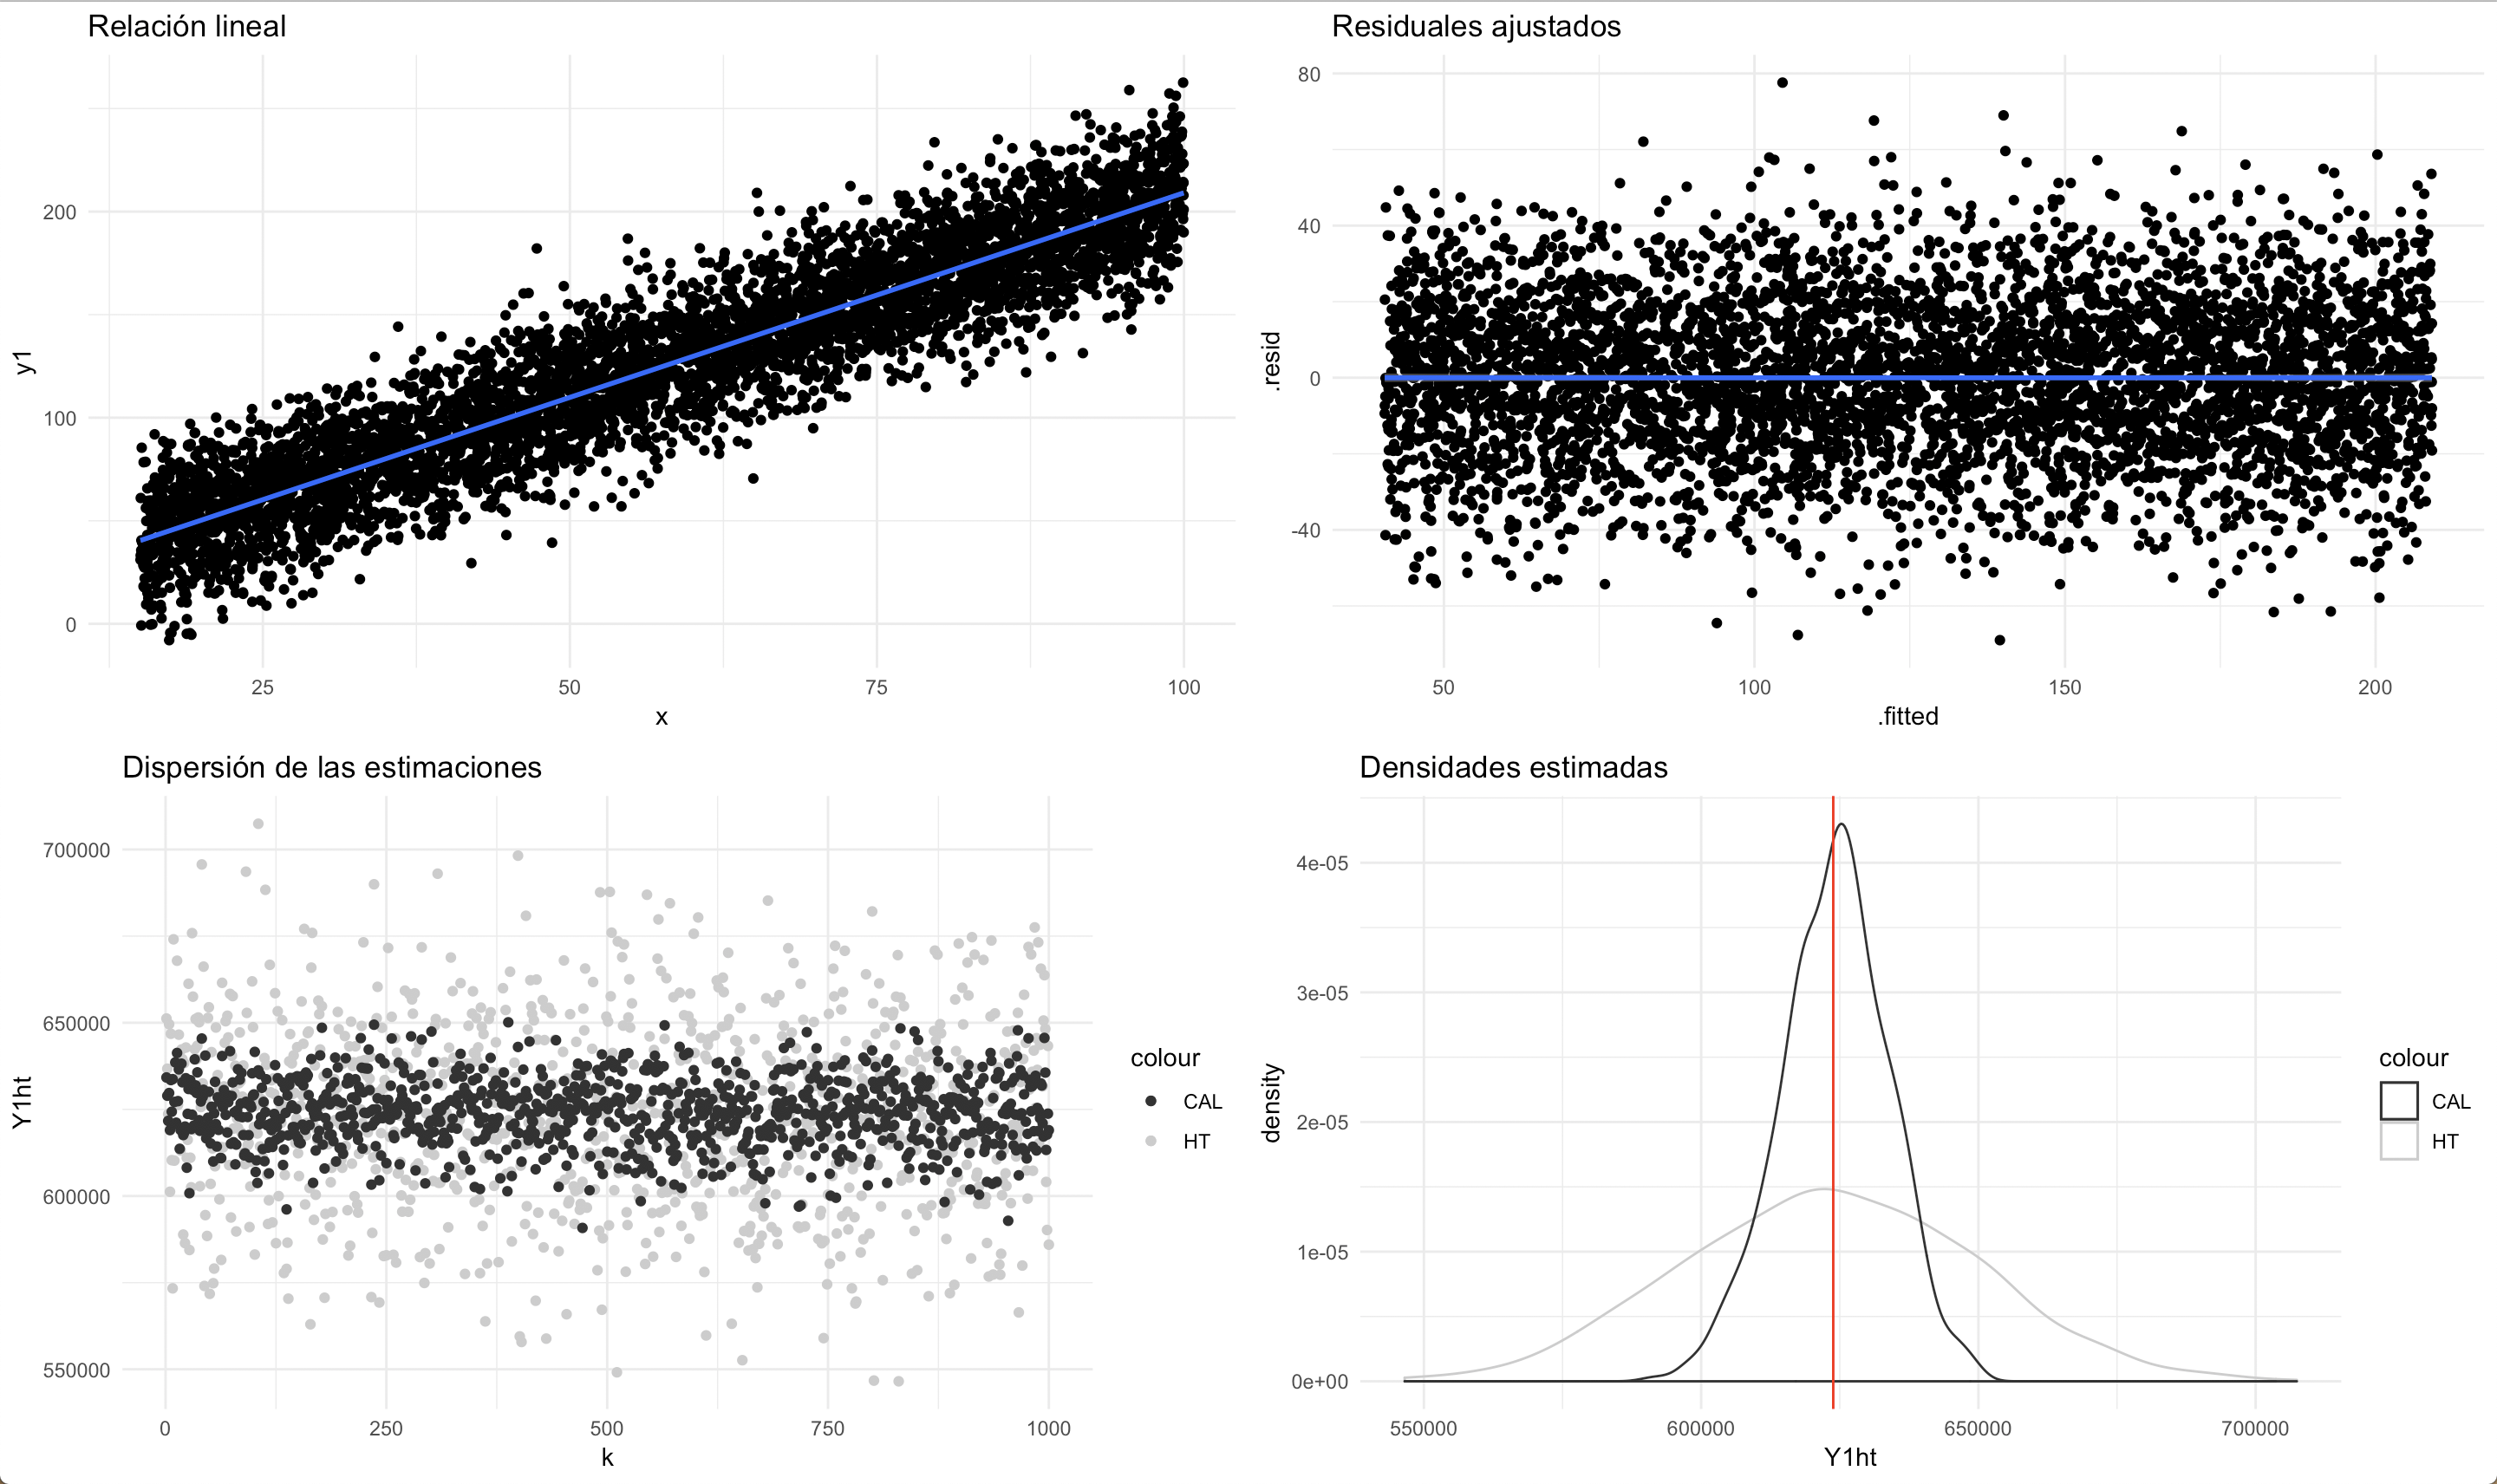
\includegraphics{Pics/c5.png}
\caption{\emph{Comportamiento del estimador de calibración en una relación de dependencia lineal}}
\end{figure}

Para el primer conjunto de datos, se supuso que existe una relación lineal entre la característica de interés y una variable de información auxiliar continua. Se nota que existe homoscedasticidad en el modelo y que los residuales tienen un comportamiento coherente. A pesar de que ambos estimadores se muestran insesgados para el parámetro de interés, se nota que el estimador de calibración es menos disperso y más eficiente.

\begin{figure}
\centering
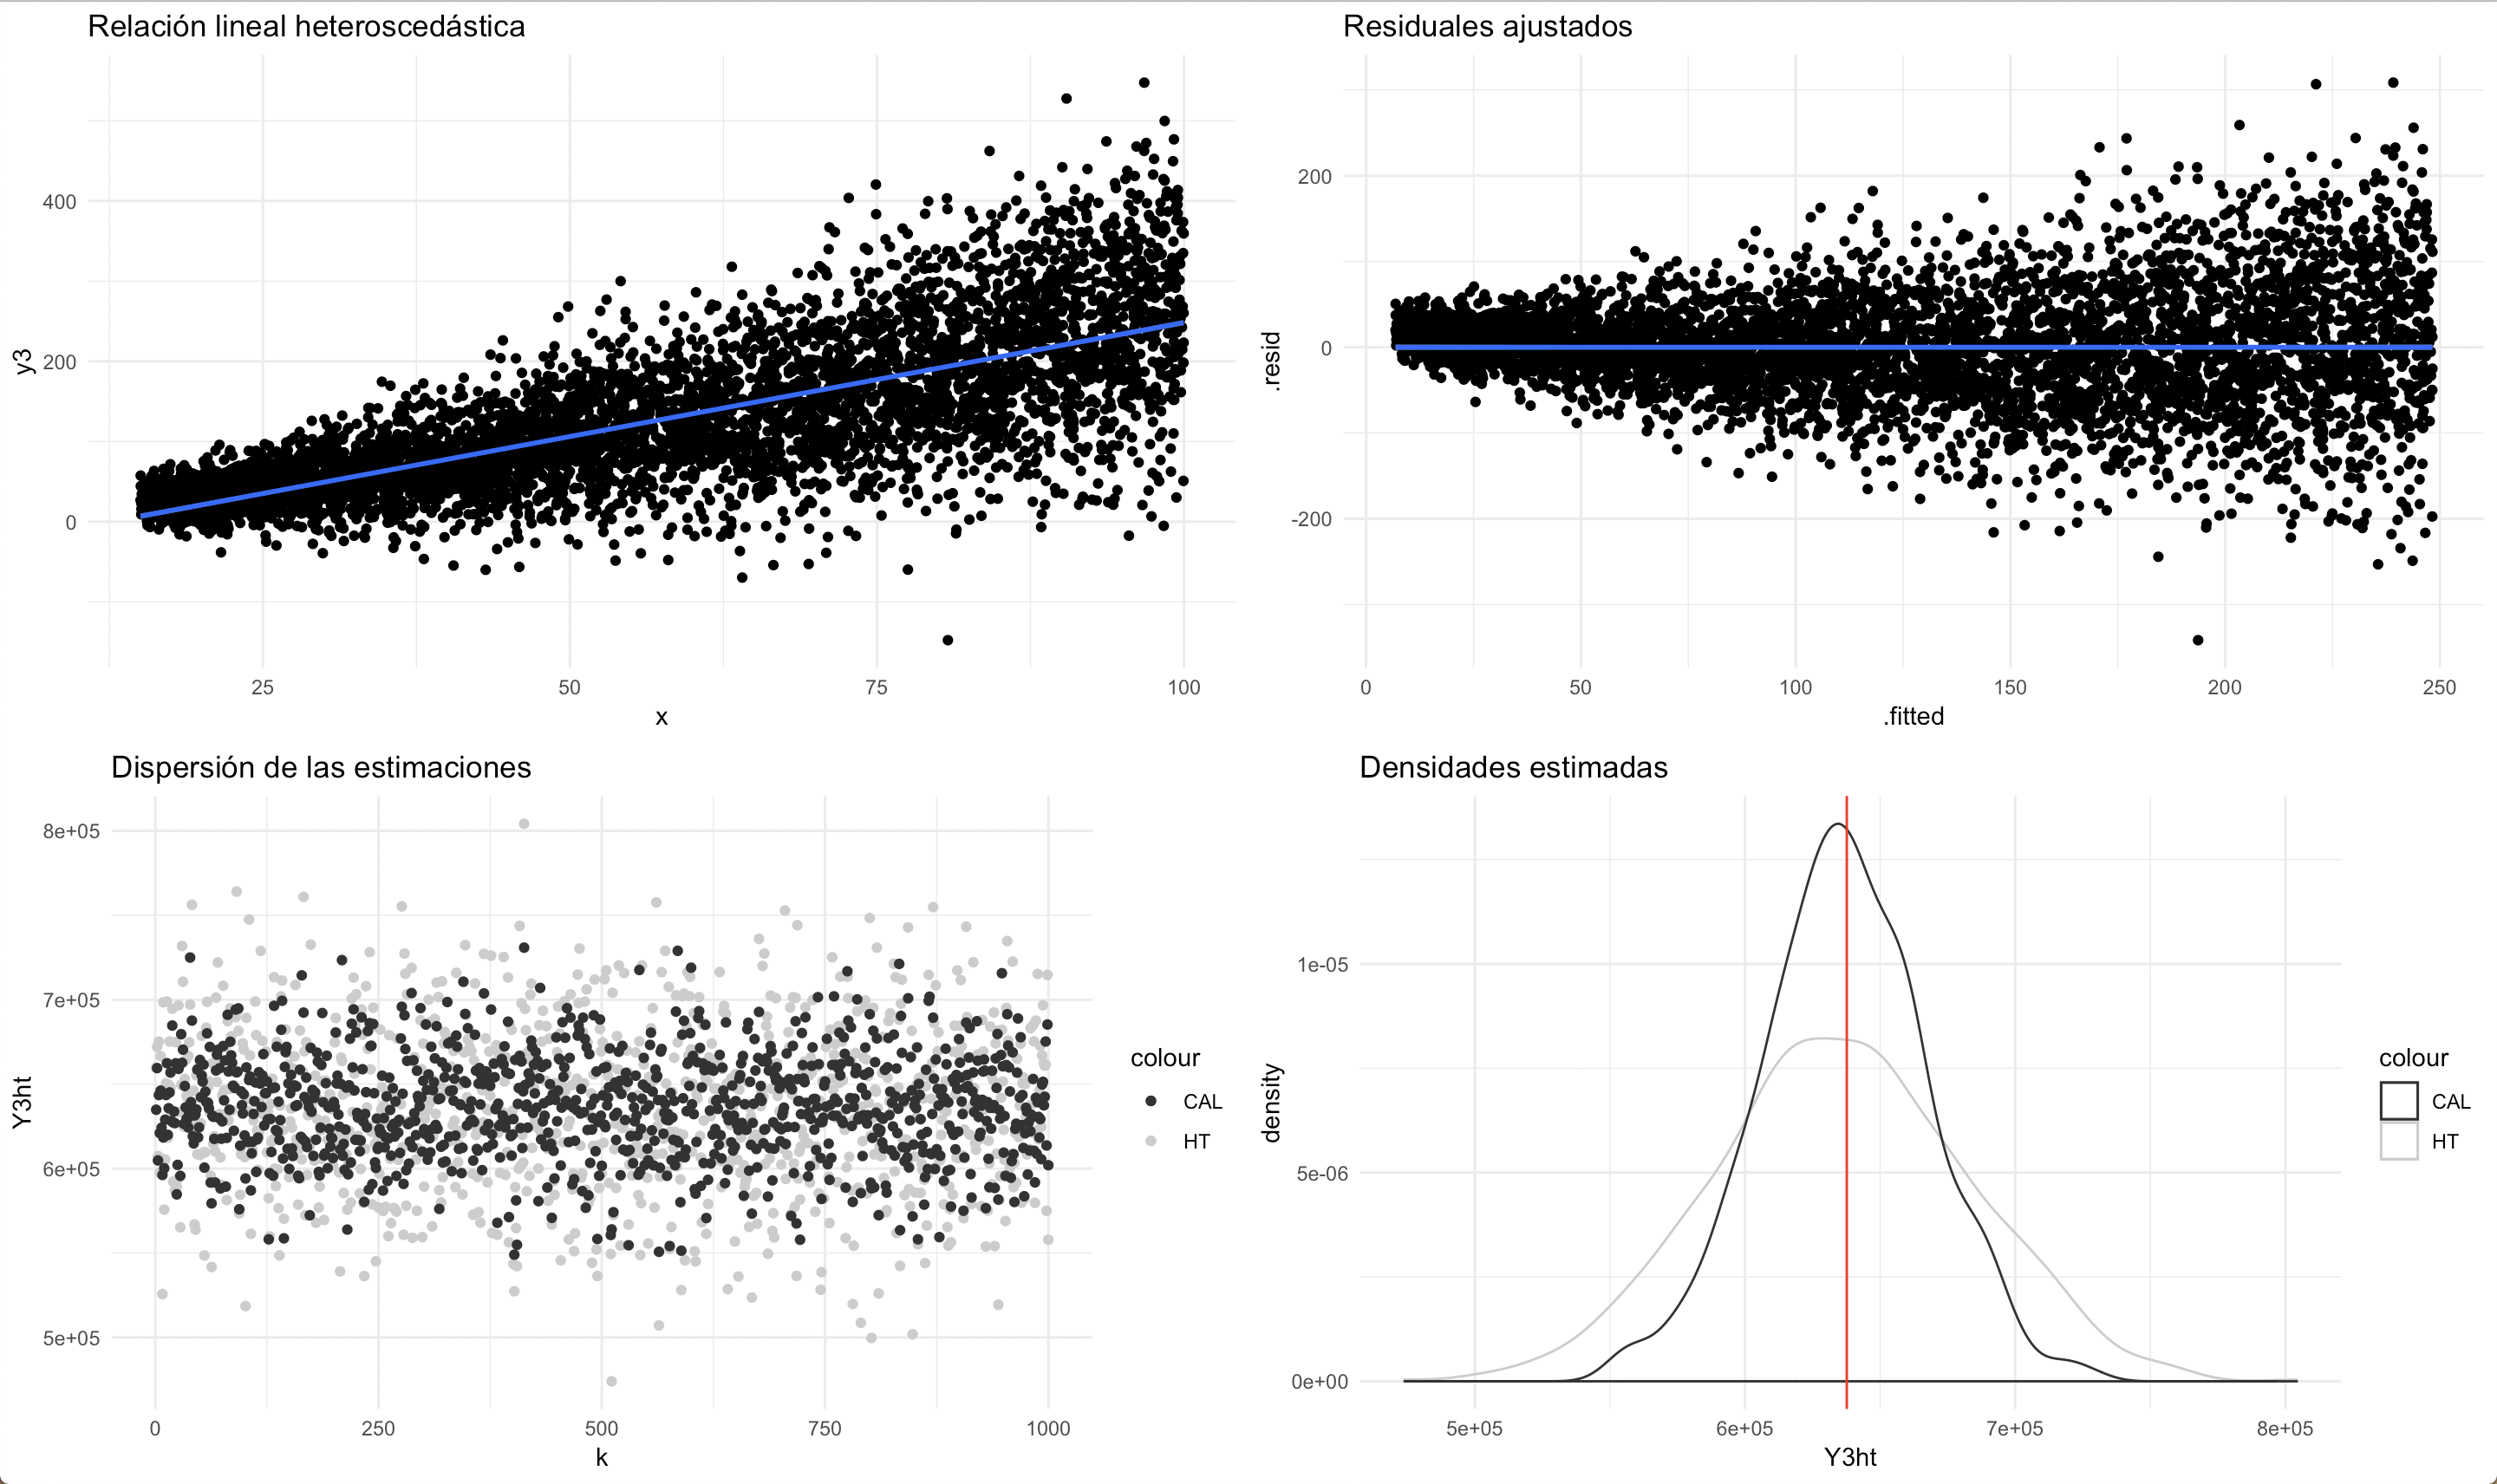
\includegraphics{Pics/c6.png}
\caption{\emph{Comportamiento del estimador de calibración en una relación de dependencia lineal con heteoscedasticidad}}
\end{figure}

El segundo conjunto de datos asume que existe una relación lineal entre la característica de interés y una variable de información auxiliar continua. Se nota que existe heteroscedasticidad en el modelo y los residuales lo muestran. A pesar de que ambos estimadores se muestran insesgados para el parámetro de interés, el estimador de calibración es un poco más eficiente que el de Horvitz-Thompson.

\begin{figure}
\centering
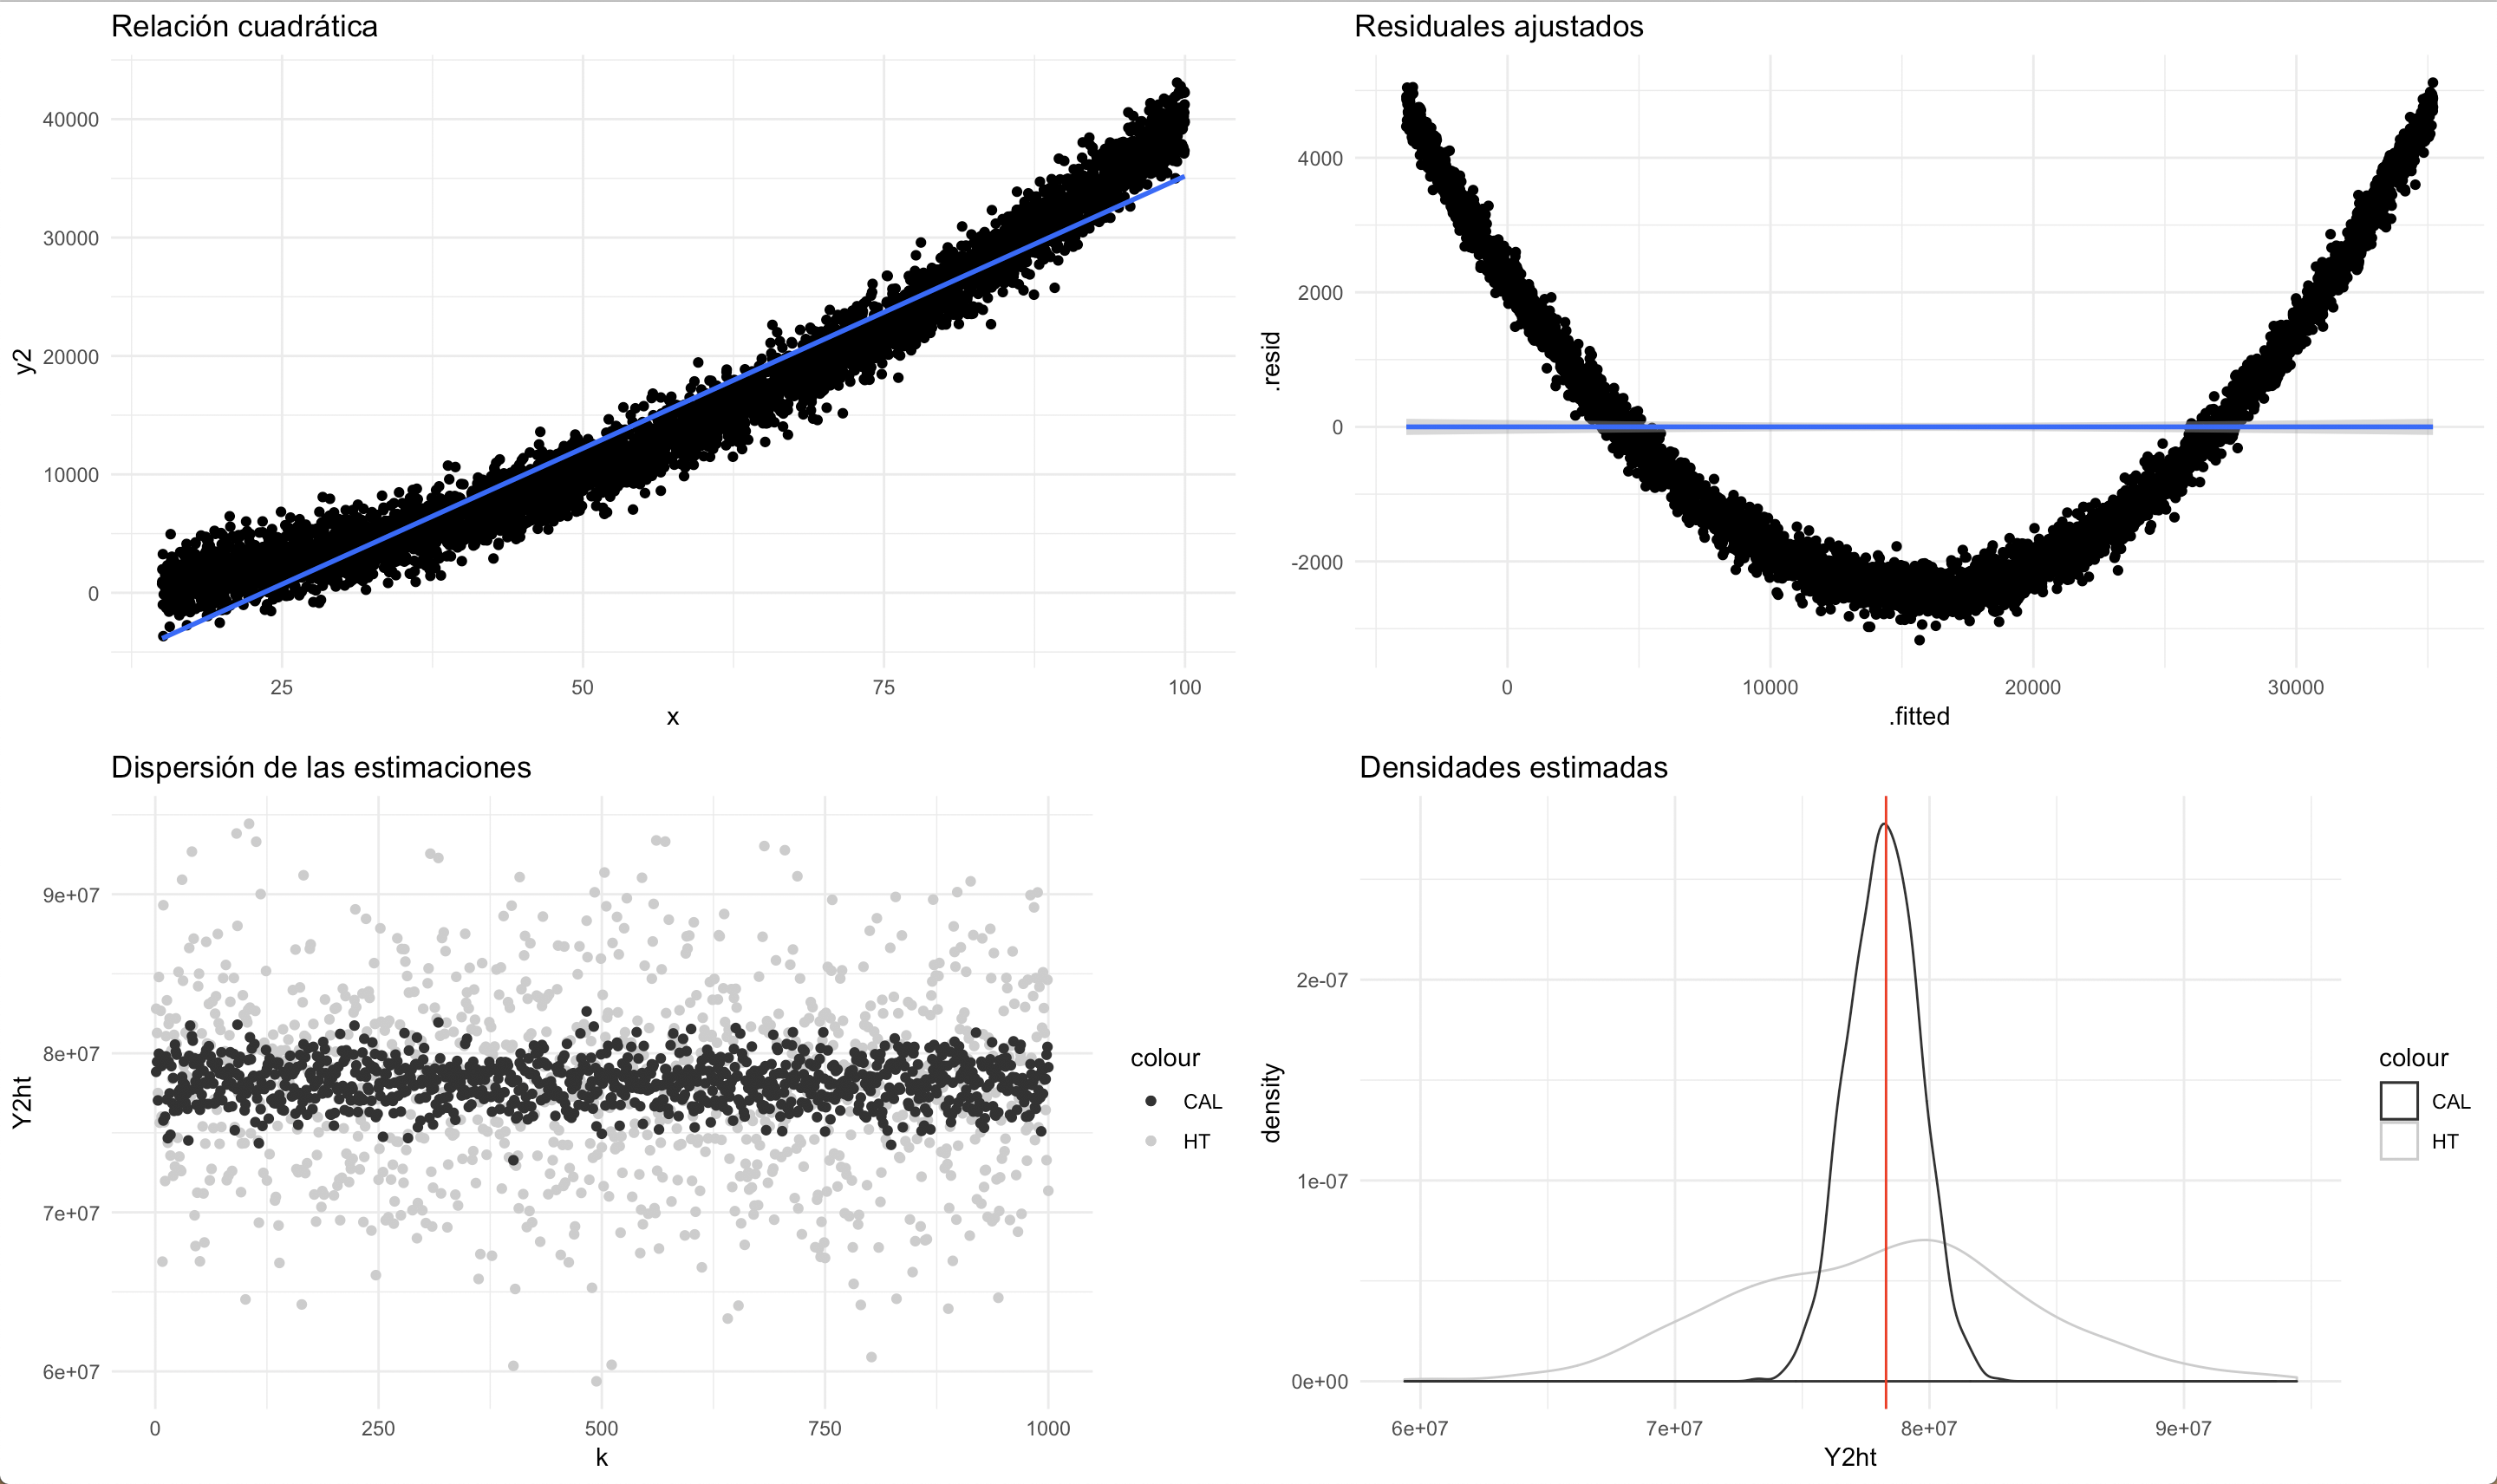
\includegraphics{Pics/c7.png}
\caption{\emph{Comportamiento del estimador de calibración en una relación de dependencia cuadrática}}
\end{figure}

Para el tercer conjunto de datos asume que existe una relación cuadrática entre la característica de interés y una variable de información auxiliar continua. Al utilizar un estimador de calibración lineal, los residuales muestran un comportamiento inapropiado. Sin embargo, ambos estimadores se muestran insesgados para el parámetro de interés, pero el estimador de calibración es más eficiente que el de Horvitz-Thompson.

\begin{figure}
\centering
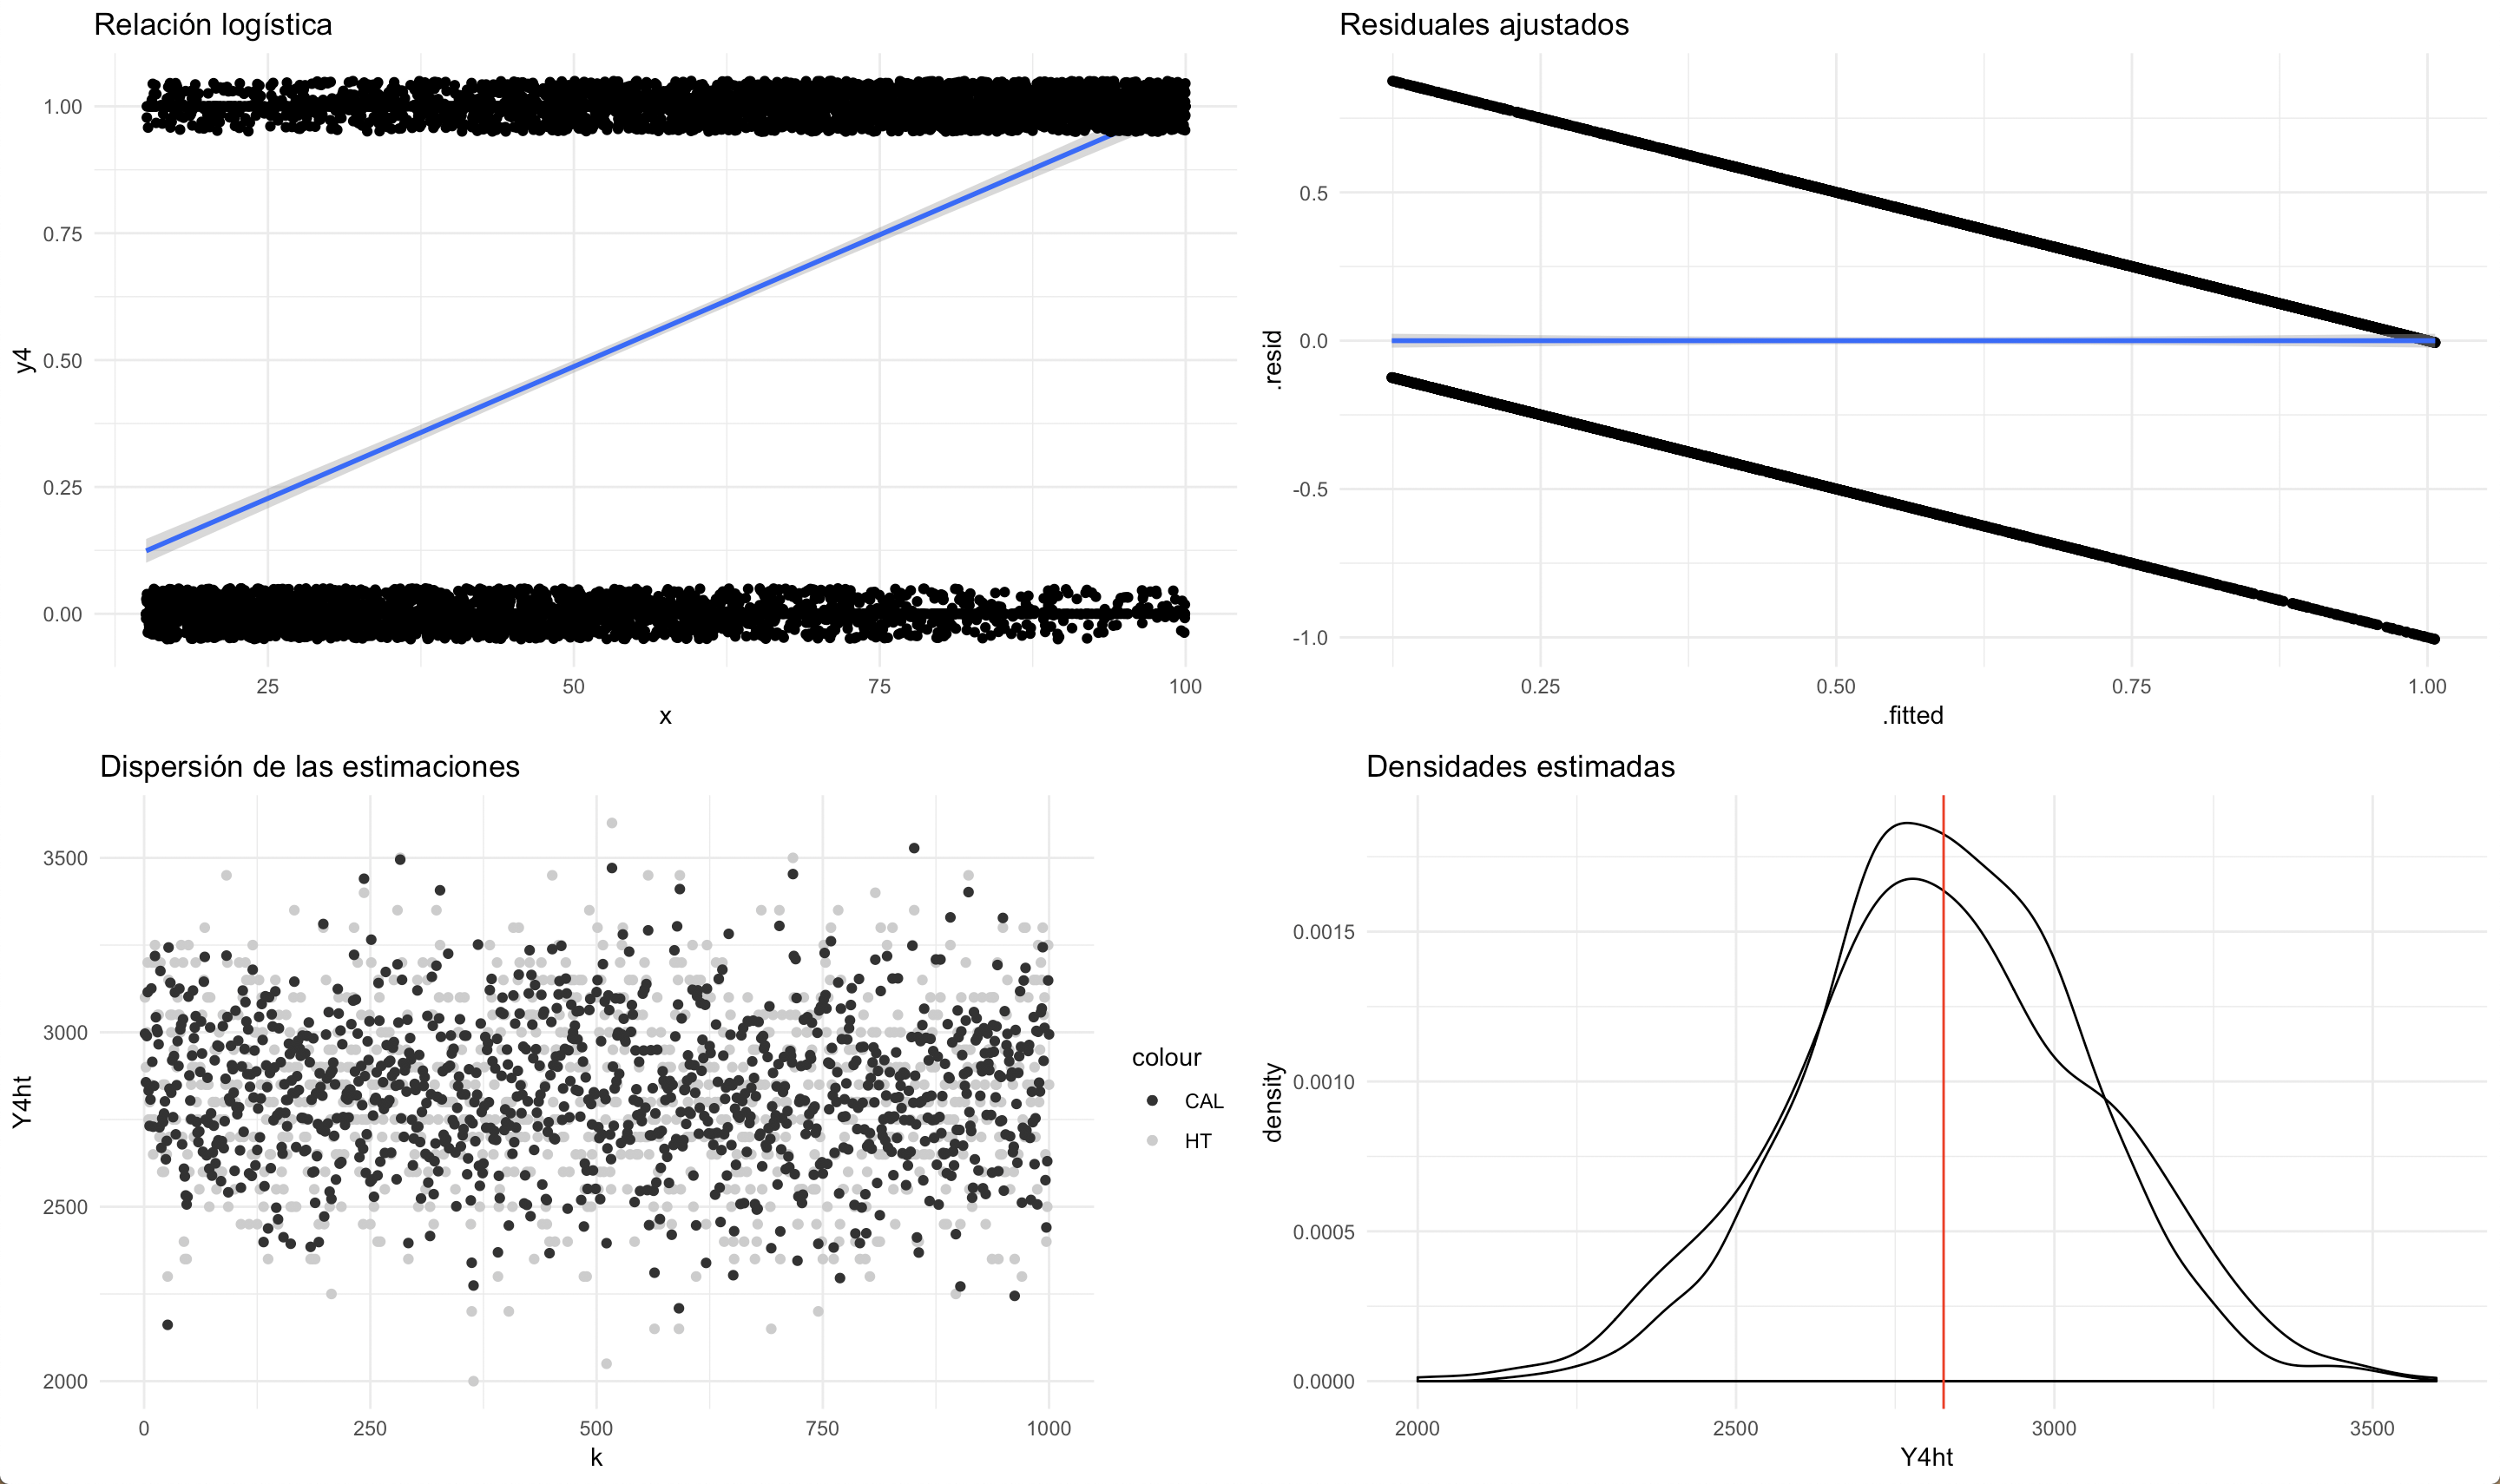
\includegraphics{Pics/c8.png}
\caption{\emph{Comportamiento del estimador de calibración en una relación de dependencia logística}}
\end{figure}

El último conjunto de datos asume que existe una relación logística entre la característica de interés y una variable de información auxiliar dicotómica Al utilizar un estimador de calibración lineal, los residuales muestran un comportamiento inapropiado. Ambos estimadores se muestran insesgados para el parámetro de interés e igual de eficientes.

¿Por qué siempre se mejora la eficiencia? Es posible demostrar que la razón entre la varianza del estimador de calibración con la varianza del estimador de Horvitz-Thompson está supeditada al coeficiente de determinación \(R^2_{\xi}\) en un modelo de regresión lineal simple \(\xi\) entre la característica de interés y la información auxiliar.

\[
\frac{Var(\hat t_{y, cal})}{Var(\hat t_{y, HT})} = (1-R^2_{\xi} + o(\sqrt{n})) \approx (1-R^2_{\xi})
\]

Por ende, usar la metodología de calibración supone casi siempre una ganancia en la eficiencia de la estrategia de muestreo.

\hypertarget{diferentes-formas-del-estimador-de-calibraciuxf3n}{%
\subsection{Diferentes formas del estimador de calibración}\label{diferentes-formas-del-estimador-de-calibraciuxf3n}}

La calibración es un ajuste que se realiza a los pesos de muestreo con el propósito de que las estimaciones de algunas variables de control reproduzcan de forma perfecta los totales poblacionales de estas variables. Sin embargo, es necesario tener en cuenta las diferencias entre los diferentes métodos de calibración, que en general corresponderán con el nivel de desagregación de información auxiliar:

\begin{enumerate}
\def\labelenumi{\arabic{enumi}.}
\tightlist
\item
  Calibración con variables continuas, que es el caso en donde la calibración se realiza con totales de variables continuas como ingreso o gasto, entre otras.
\item
  Post-estratificación con variables categóricas, que representa el caso en donde la calibración se realiza con los tamaños poblacionales (basados en proyecciones demográficas o registros administrativos) de subgrupos de interés.
\item
  \emph{Raking} con variables categóricas, que se define como una calibración sobre los tamaños marginales de tablas de contingencia de subgrupos de interés. A diferencia del caso anterior, esta calibración no tiene en cuenta los tamaños de los cruces, sino solo los tamaños marginales; por ende, este método induce menos restricciones.
\end{enumerate}

\hypertarget{postestratificaciuxf3n}{%
\subsubsection*{Postestratificación}\label{postestratificaciuxf3n}}
\addcontentsline{toc}{subsubsection}{Postestratificación}

La postestratificación es una de las técnicas más usadas para el ajuste de los pesos de muestreo vía calibración. Este ajuste requiere la definición de categorías poblacionales. Por ejemplo, personas en un determinado grupo de edad, en cierta región y de cierta razan. Este método se se implementa dentro de cada uno de los cruces inducidos por las covariables de interés (edad X región X raza). Nótese que es necesario tener acceso a la información auxiliar a nivel de \emph{todos} los cruces definidos por los subgrupos. Usualmente corresponden a proyecciones demográficas. En este caso, la suma de los pesos ajustados reproducirán con exactitud los tamaños poblacionales en cada cruce.

Las categorías formadas para definir los pesos de muestreo se conocen como \emph{post-estratos} puesto que son definidas después de que la muestra es seleccionada y los datos son recolectados. Esta es una ventaja pues estas variables no necesariamente participan en la planificación del diseño de muestreo. Por ejemplo, en una encuesta de hogares es difícil estratificar por raza, edad, sexo o ciclo educativo alcanzado. Como se conoce que estas variables pueden estar correlacionadas con la pobreza, el ingreso o la ocupación, sería una buena idea contemplarlas en la calibración.

De esta manera, siendo \(g = 1, \ldots, G\) el indicador del cruce poblacional (post-estrato), el estimador de postestratifiación queda definido de la siguiente manera:

\[
\hat{t}_{y, pos} = \sum_{g = 1}^G \frac{N_g}{\hat{N}_g}\hat{t}_{y_g}
\]

En donde \(N_g\) corresponde al tamaño poblacional del post-estrato, \(\hat{N}_g = \sum_{s_g} d_{k}\) y \(\hat{t}_{y_g} = \sum_{s_g} d_{k} y_k\). Por lo anterior, el factor de expansión de estimador postestratificado queda definido como sigue:

\[
w_k= d_k \frac{N_g}{\hat{N}_g} \ \ \ \ \ \forall \ k \in s_g
\]

Note que \(d_k\) corresponde al peso inducido por el diseño de muestreo, corregido por los ajustes de elegibilidad y por la ausencia de respuesta.

Por último, se debe considerar que la cantidad de postestratos en la calibración está inducido por la cantidad de interacciones en las variables auxiliares. En algunos casos, es posible encontrar cientos de interacciones. Aunque los tamaños de los postestratos se reproduce sin error, esto puede decrecer la eficiencia de la calibración en las variables de interés. Es decir que, muchas variables e interacciones hacen que las estimaciones sean inestables, sobre todo si existen cruces con celdas vacías. Es posible que el efecto de las interacciones influencie la creación de los nuevos pesos calibrados y se tengan outliers en los pesos de calibración resultantes.

\hypertarget{raking}{%
\subsubsection*{Raking}\label{raking}}
\addcontentsline{toc}{subsubsection}{Raking}

¿Qué sucede si los conteos poblacionales (información auxiliar) no están disponibles para todos los cruces de las variables de calibración? Es posible que los agregados poblacionales de las variables provengan de distintas fuentes y no se pueda llegar a nivel de cruce. En este caso, es factible calibrar los marginales de la tabla cruzada, sin necesidad de calibrar todas sus entradas. En este caso, el número de restricciones decrecería con respecto a la postestratifación, pues se sumaría el número de categorías, mientras que en la postestratificación se multiplican.

Para ajustar los marginales de la tabla cruzada, es necesario realizar un procedimiento iterativo (IPFP), el cual no tiene una escritura cerrada \citep[capítulo 10]{Gutierrez_2016}. Por ejemplo, si el \emph{raking} es de dos marginales, se ajustan primero las filas, luego las columnas y así sucesivamente hasta alcanzar la convergencia de los pesos calibrados y el procedimiento se detiene cuando se alcanza una tolerancia prefijada.

En general, los pesos calibrados se escriben de la siguiente manera:

\[w_k = d_k \times exp(u_h) \times exp(v_g)\]
En donde \(u_h\) es una función de los totales marginales de las filas de la tabla cruzada y \(v_g\) es una función de los totales marginales de las columnas. El \emph{raking} permite utilizar variables que pueden ser predictoras de las variables de interés o explicar la probabilidad de responder del hogar (o persona), además de mejorar las tasas de cobertura del marco de muestreo.

\hypertarget{la-calibraciuxf3n-como-un-cambio-de-paradigma}{%
\subsection{La calibración como un cambio de paradigma}\label{la-calibraciuxf3n-como-un-cambio-de-paradigma}}

\citet{Sar08} concluye que existen algunas ideas sobre las cuales vale la pena profundizar un poco más. A continuación se reproducen las ideas de \citet{Gutierrez_2016} sobre estos criterios para enfatizar el uso práctico de los estimadores de calibración:

\begin{enumerate}
\def\labelenumi{\arabic{enumi}.}
\item
  La calibración tiene un vínculo íntimo con la práctica. La fijación con métodos de ponderación de las agencias que manejan las estadísticas oficiales es una poderosa costumbre que empezó con la ponderación de unidades mediante el inverso de su probabilidad de inclusión y siguió con las ponderaciones surgidas del enfoque de post-estratificación. Las ponderaciones de calibración extienden las anteriores ideas. La calibración es reciente como término en el muestreo, pero no lo es como técnica para producir ponderaciones. Algunos autores derivaron estas ponderaciones con el argumento de que deberían diferir de la manera más mínima posible de los pesos originales. Otros autores encontraron las ponderaciones al reconocer que un estimador de regresión lineal podría ser escrito como una suma ponderada de los valores de la característica de interés. De allí surgieron términos tales como ponderación de muestreo, ponderación de regresión y ponderación de caso.
\item
  En algunas ocasiones el término calibración se refiere a una forma de conseguir estimativos consistentes\footnote{En este apartado la palabra consistente se da en el sentido de la consistencia con los totales de la información auxiliar.}. Las ecuaciones de calibración imponen esta propiedad de consistencia sobre el vector de ponderaciones; así que, cuando éste se aplica a las variables auxiliares el resultado será consistente con los totales de estas variables. Un deseo de promover la credibilidad en las estadísticas oficiales es una razón para que las entidades busquen la consistencia. Cuando la motivación primaria para la calibración no es la concordancia con los totales de la información auxiliar sino el reducir la varianza y el sesgo debido a la ausencia de respuesta entonces el vector de ponderaciones se dice balanceado.
\item
  El enfoque de calibración ha ganado popularidad en las aplicaciones reales debido a que las estimaciones resultantes son fáciles de interpretar y de motivar puesto que están directamente relacionadas a los pesos inducidos por el diseño de muestreo. La calibración sobre los totales conocidos brinda al usuario una forma natural y transparente de estimación. El usuario que entiende la ponderación muestral aprecia el método de calibración puesto que modifica sutilmente los pesos originales, pero al mismo tiempo respeta los totales de la información auxiliar y mantiene el sesgo despreciable. Además, en la mayoría de aplicaciones, la calibración induce un único vector de ponderaciones aplicable a todas las variables involucradas en el estudio. Esta última razón hace que este método sea muy apetecido en las entidades oficiales que manejan encuestas muy extensas.
\item
  Algunos autores usan la palabra calibración en combinación con otros términos para describir varias direcciones de pensamiento. Por ejemplo, es posible encontrar términos como calibración de modelo, calibración G, calibración armonizada, calibración a un nivel más alto, calibración de regresión, calibración no lineal, calibración super-generalizada, calibración de modelos de redes neuronales, calibración basada en modelos locales polinomiales, entre otras.
\item
  Si la calibración representa un nuevo enfoque demarcado claramente de sus predecesores, entonces es tiempo de hacer la pregunta: ¿La calibración generaliza las teorías anteriores? ¿La calibración da mejores respuestas a las preguntas de importancia, que los enfoques de estimación anteriores? En la práctica el estadístico encuentra algunos pormenores tales como ausencia de respuestas, deficiencias del marco muestral y errores de medición. Es cierto que algunos procesos como la imputación y la reponderación para no respuestas son ampliamente difundidos y usados en la práctica. Sin embargo queda un sinsabor al utilizar estos métodos pues no están enmarcados dentro de una teoría exhaustiva de inferencia en poblaciones finitas. La mayoría de artículos teóricos tratan con la estimación de parámetros bajo un mundo ideal, que no existe en la práctica, donde la ausencia de respuesta y otros errores no muestrales están ausentes.
\end{enumerate}

\hypertarget{construcciuxf3n-de-los-factores-de-expansiuxf3n}{%
\chapter{Construcción de los factores de expansión}\label{construcciuxf3n-de-los-factores-de-expansiuxf3n}}

En todas las bases de datos de las encuestas de hogares se encuentra una columna que contiene los pesos de muestreo o factores de expansión. Con esta columna se realizan todos los análisis requeridos en la encuesta, desde estimar medias, razones, tamaños y proporciones hasta el ajuste de modelos lineales y no lineales.

La razón principal por la cual se usan los factores de expansión es para producir estimaciones que reflejen de manera precisa el comportamiento de la población objetivo. El uso de los factores de expansión garantiza que:

\begin{itemize}
\tightlist
\item
  La estimación sea insesgada y consistente.
\item
  El error de muestreo sea pequeño, condicionado al diseño muestral y al tamaño de la muestra.
\item
  Las deficiencias de cobertura del marco sean corregidas.
\end{itemize}

Los procesos de inferencia estadistica establecidos en cualquier encuesta de hogares descansan sobre el principio de representatividad que afirma que es posible seleccionar una muestra y representar con bastante precisión y exactitud la realidad de la población de interés. A su vez, las propiedades estadísticas de la inferencia en encuestas de hogares descansan sobre las probabilidades de inclusión generadas por el diseño de muestreo que se implementó en la encuesta. En general el peso de muestreo \(d_k\) asociado a un individuo \(k\) en la muestra \(s\) es una función del inverso de la probabilidad de inclusión del individuo, así

\[
d_k \propto \frac{1}{Pr(k\in s)}
\]

Como se mencionó anteriormente, para conservar estabilidad en los pesos de muestreo, es posible definir diseños de muestreo auto-ponderados, en donde las unidades finales de muestreo tengan las misma probabilidad de inclusión, sin importar el tamaño de la unidad primaria de muestreo que la contiene. Este tipo de diseños es útil porque induce mayor control sobre las estimaciones finales. Además, los pesos de muestreo se utilizan con el fin de

\begin{enumerate}
\def\labelenumi{\arabic{enumi}.}
\tightlist
\item
  Incorporar las probabilidades de selección de las unidades en la muestra.
\item
  Ajustar en casos en los que no se pueda determinar si algunas unidades en la muestra son miembros de la población de interés.
\item
  Minimizar el sesgo causado por la ausencia de respuesta cuando algunas unidades no responden habiendo sido incluidas en la muestra.
\item
  Incorporar información auxiliar externa para reducir los errores muestrales de las estimaciones.
\item
  Compensar cuando la muestra no cubre correctamente a la población de interés.
\end{enumerate}

Es de notar que la conformación de los pesos de muestreo se transforma en un reto metodológico para el investigador, puesto que debe ajustarse a la realidad de la región en donde las poblaciones de los municipios se expanden cada vez más en el sector urbano y los marcos de muestreo de las áreas geográficas se desactualizan con rapidez. Varias soluciones a este problema han sido planteadas \citep{Gambino_Silva_2009} y todas ellas requieren de esfuerzos económicos, logísticos y técnicos. Por ende, los equipos de los INE (a todo nivel) deben ser flexibles y adecuarse a esta realidad cambiante de la movilidad de las poblaciones, sobre todo en las áreas urbanas.

En condiciones ideales el marco de muestreo debería coincidir plenamente con la población finita. Sin embargo, en general, no es posible contar con una lista de todos los elementos de la población y, en el contexto de las encuestas a hogares, no existe una lista que enumere todos los hogares de un país de manera actualizada, por lo que la práctica estándar es construir el marco de muestreo en varias etapas, seleccionando una muestra de áreas geográficas, realizando un empadronamiento exhaustivo de todos los hogares en las áreas seleccionadas y luego seleccionando hogares. Este esquema de muestreo hace que el marco de muestreo de las encuestas a hogares presente imperfecciones.

Para hacerle frente a las imperfeccciones del marco, \citet{Valliant_Dever_2017} recomienda el uso de los códigos de disposición estandarizados por la \emph{American Association for Public Opinion Research} (AAPOR) recomienda tratar la ausencia de respuesta de manera diferenciada y clasificar a cada unidad en la muestra en algunas de las siguientes categorías:

\begin{enumerate}
\def\labelenumi{\arabic{enumi}.}
\tightlist
\item
  ER (\emph{unidades elegibles que fueron respondientes efectivos}): casos elegibles para los cuales se ha recolectado una cantidad suficiente de información.
\item
  ENR (\emph{unidades eligibles no respondientes}): casos elegibles para los cuales no se recolectó ningún dato o la información fue parcialmente recolectada.
\item
  IN (\emph{unidades no elegibles}): casos de miembros no elegibles que no hacen parte de la población de interés.
\item
  UNK (\emph{unidades con elegibilidad desconocida}): casos en donde no se puede conocer si la unidad es elegible o no.
\end{enumerate}

Para construir los factores de expansión de una encuesta se recomienda seguir en este orden los siguientes procesos:

\begin{enumerate}
\def\labelenumi{\arabic{enumi}.}
\tightlist
\item
  Creación de los pesos básicos.
\item
  Ajuste por elegibilidad desconocida.
\item
  Descarte de las unidades no elegibles.
\item
  Ajuste por ausencia de respuesta.
\item
  Calibración por proyecciones poblacionales y variables auxiliares.
\item
  Preparación de la base de datos de respondientes.
\end{enumerate}

\hypertarget{creaciuxf3n-de-los-pesos-buxe1sicos}{%
\section{Creación de los pesos básicos}\label{creaciuxf3n-de-los-pesos-buxe1sicos}}

Este primer paso ya ha sido explicado de forma detallada en la sección dedicada a la selección de la muestra. Observe que, asociado a cada esquema particular de muestreo, existe una única función que víncula a cada elemento con una probabilidad de inclusión en la muestra. De esta forma:

\[\pi_k = Pr (k \in s)\]

Por lo tanto, el primer paso, en la reponderación de los pesos de muestreo, es justamente la creación de los pesos básicos \(d_{1k}\) que se definen como el inverso multiplicativo de la probabilidad de inclusión

\[d_{1k} = \frac{1}{\pi_k}\]

Estos pesos son creados incluso para aquellas unidades que serán excluidas de la muestra porque son no elegibles o porque no proveyeron ninguna información y luego serán modificados convenientemente. La siguiente figura muestra la distribución típica de los pesos originales en una encuesta de hogares. Se recomienda calcular las probabilidades de inclusión y selección a medida que avance el muestreo en sus etapas y, de esta forma, siempre confirmar la consistencia de los pesos en cada etapa y de los pesos finales.

A través de las modificaciones posteriores sobre este peso de muestreo, la distribución de los ponderadores irá sufriendo algunos cambios. Si la distribución original de los pesos básicos difiere estructuralmente con la distribución final de los ponderadores, resultante de todos los ajustes debidos a las imperfecciones del marco, entonces las propiedades estadísticas de insesgamiento, consistencia y precisión podrían desvanecerse. Lo anterior implica que el nivel de desactualización del marco de muestreo tiene implicaciones directas en la calidad de la inferencia. Por tanto, si el marco de muestreo es muy imperfecto, los ponderadores finales no inducirán una inferencia precisa.

\begin{figure}
\centering
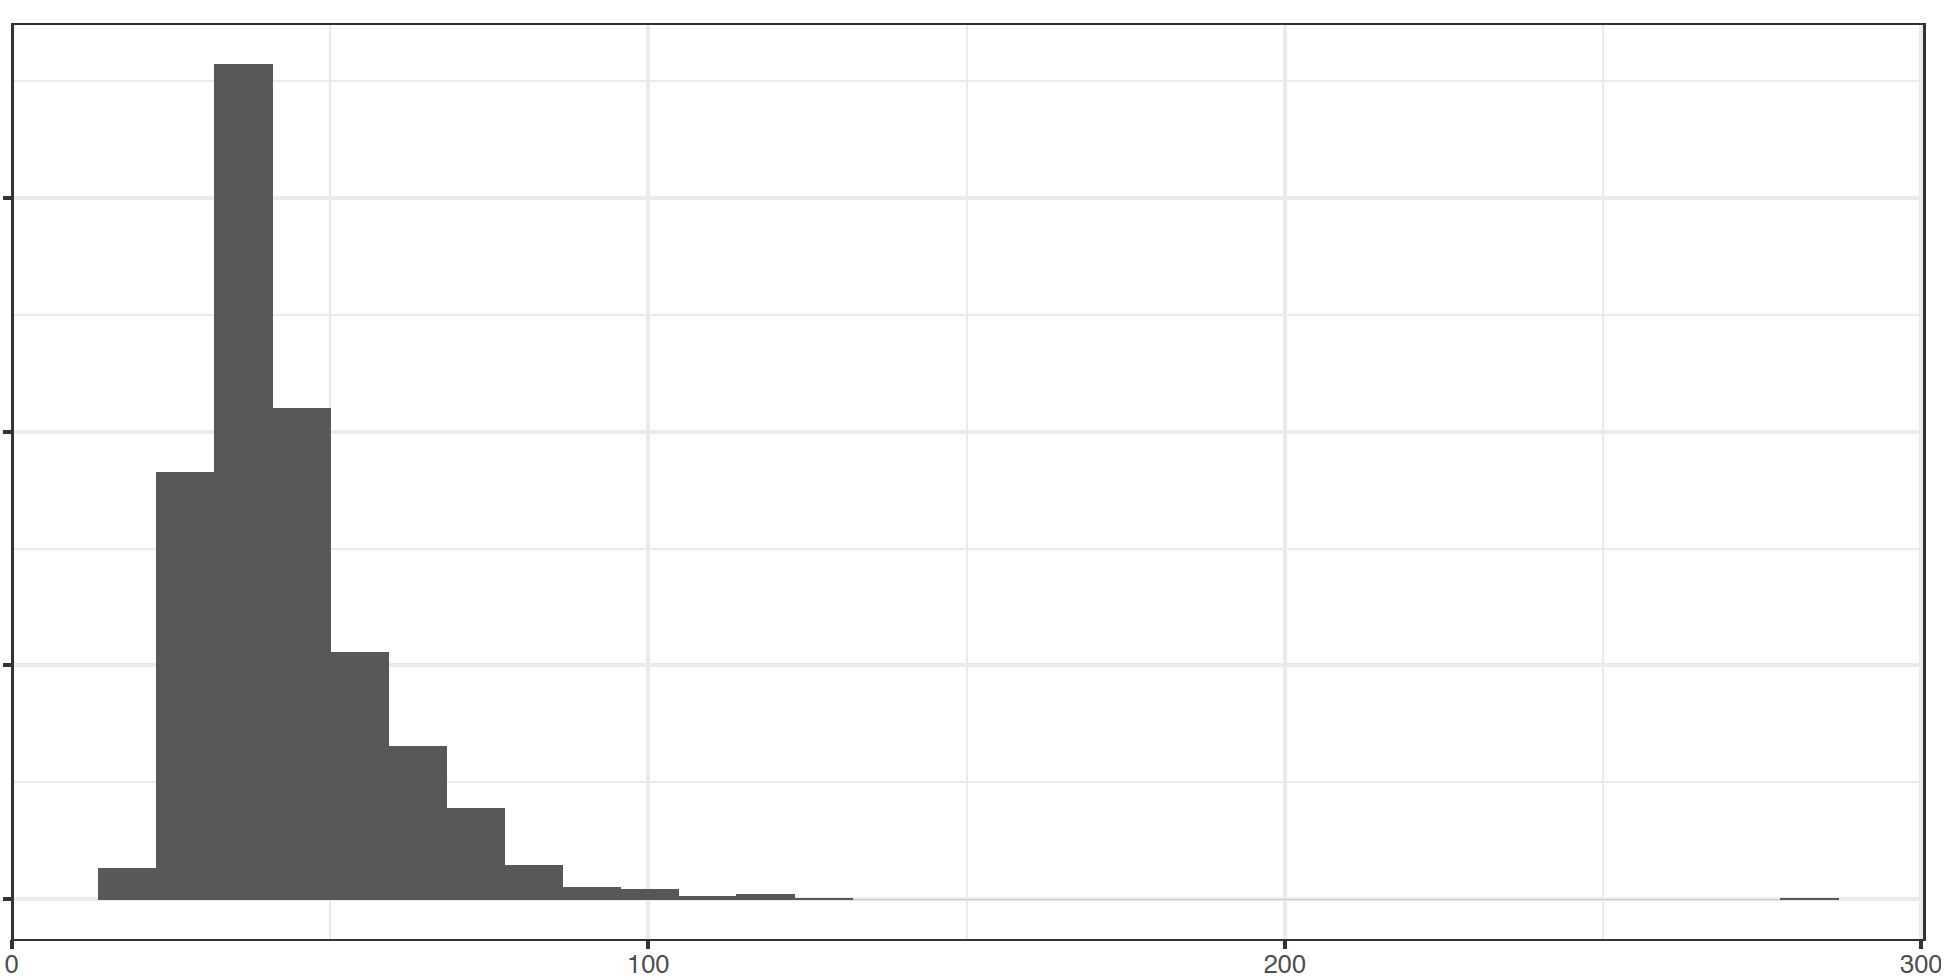
\includegraphics[width=\textwidth,height=5.20833in]{Pics/15.png}
\caption{\emph{Distribución de los pesos básicos de muestreo en una encuesta de hogares.}}
\end{figure}

\hypertarget{ajuste-por-elegibilidad-desconocida}{%
\section{Ajuste por elegibilidad desconocida}\label{ajuste-por-elegibilidad-desconocida}}

El tercer paso consiste en redistribuir el peso de las unidades cuyo estado de elegibilidad es desconocido. Por ejemplo, si la encuesta está enfocada en la población mayor de 15 años y hay personas que no proveen ninguna información acerca de su edad, entonces es necesario distribuir estos pesos. Esta situación también se puede presentar a nivel de hogar cuando no puede ser contactado porque nadie nunca atendió el llamado del encuestador (\emph{nadie en casa}). Se acostumbra a redistribuir los pesos de los UNK entre las unidades que sí disponen de su estatus de elegibilidad (ER, ENR, IN).

Es así como, si no es posible determinar la elegibilidad de algunas unidades que aparecen en el marco de muestreo, se tendrá una muestra \(s\) que contendrá el conjunto de las unidades \emph{elegibles} en la muestra \(s_{e}\), el conjunto de las unidades \emph{no elegibles} en la muestra \(s_{n}\) y el conjunto de las unidades con \emph{elegibilidad desconocidad} \(s_{u}\). En este último caso, la elegibilidad de estos casos es desconocida, a no ser que de manera arbitraria sean clasificadas como ENR (elegibles no respondientes), o se tenga información auxiliar en el marco de muestreo que permita imputar su estado de elegibilidad.

Se recomienda formar \(B\) \((b = 1, \ldots, B)\) categorías\footnote{Se acostumbra a formar categorías con al menos 50 casos.} basadas en la información del marco de muestreo. Estas categorías pueden ser estratos o cruces de subpoblaciones. Siendo \(s_b\) la muestra de unidades en la categoría \(b\) (que incluye a ER, ENR y UNK), se define el factor de ajuste por elegibilidad como:

\[
a_b = \frac{\sum_{s_b}d_{1k}}{\sum_{s_b \cap s_e}d_{1k}}
\]
Para la categoría \(b\), los pesos ajustados por elegibilidad desconocida para aquellas unidades cuya elegibilidad si pudo ser establecida (independientemente de su estado de respuesta) estarán dados por la siguiente expresión:

\[
d_{2k} = a_b * d_{1k}
\]

\begin{figure}
\centering
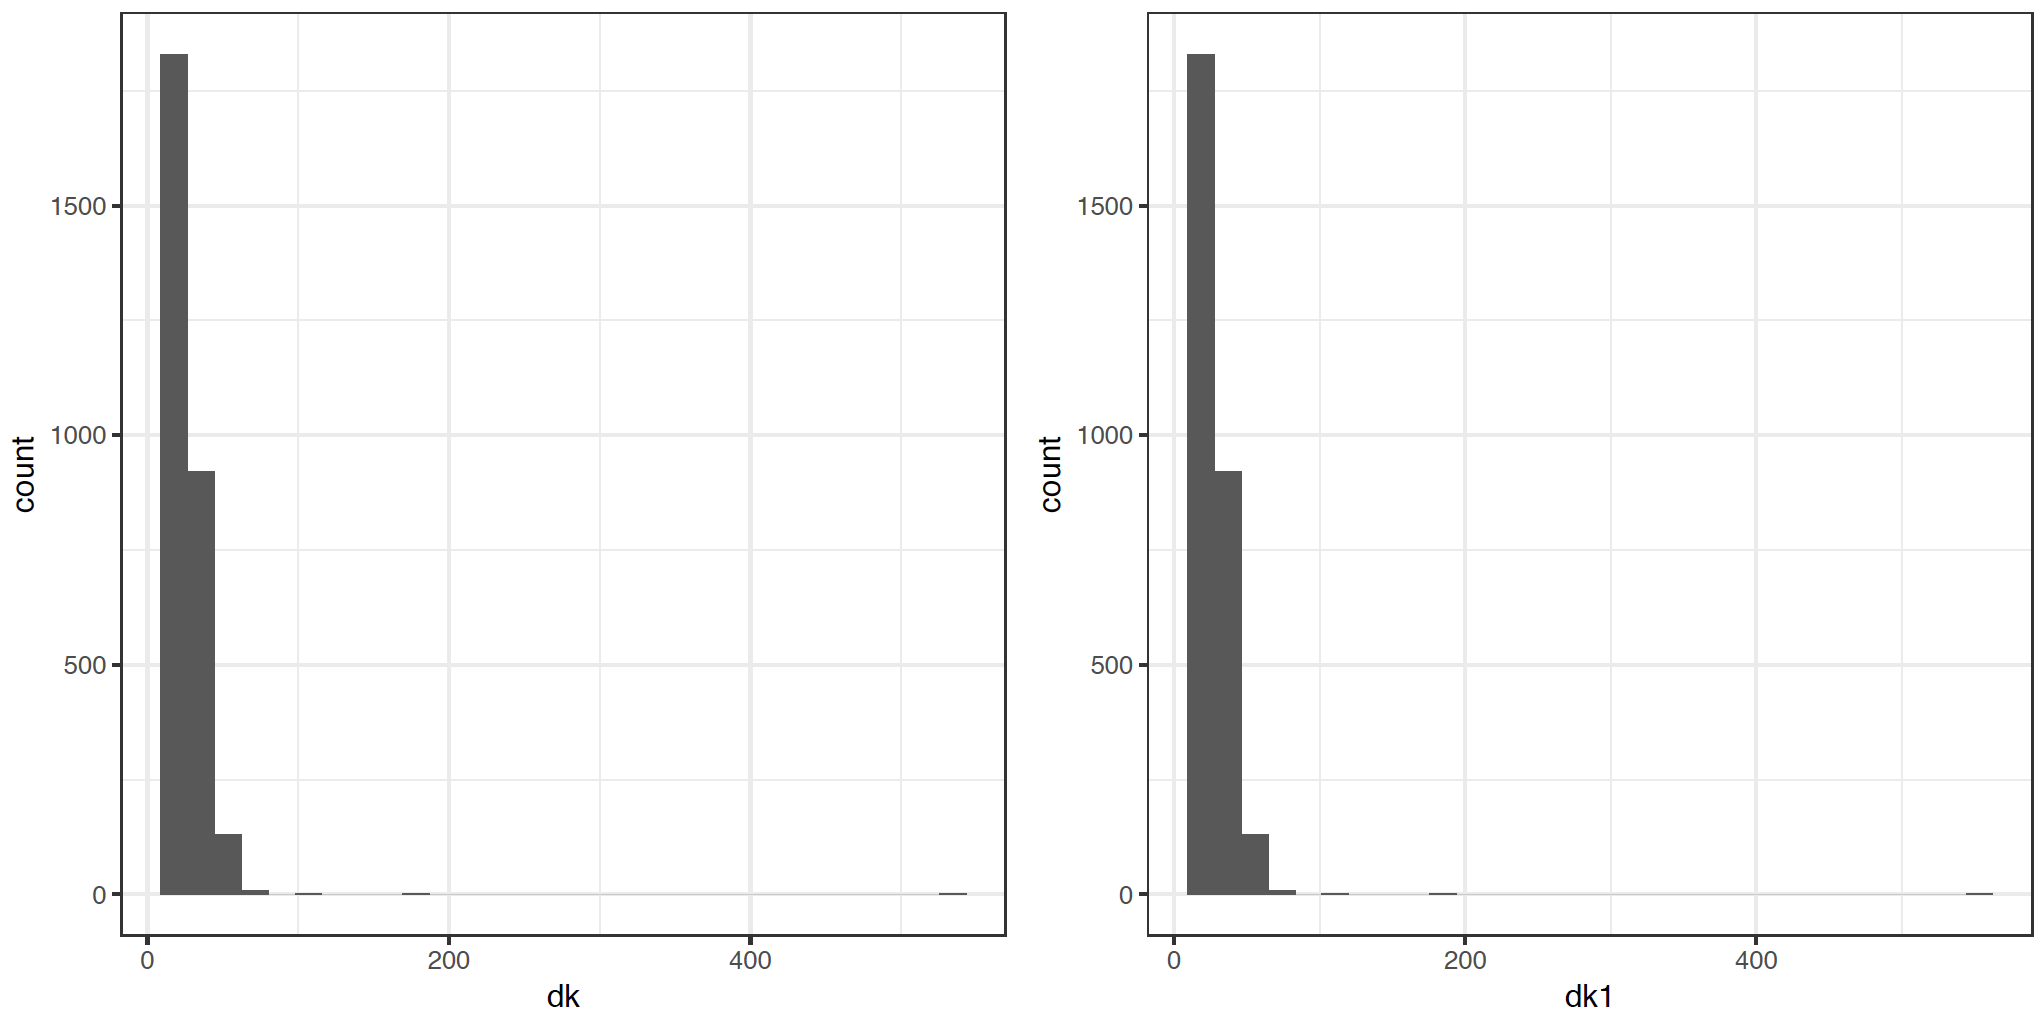
\includegraphics[width=\textwidth,height=5.20833in]{Pics/16.png}
\caption{\emph{Comparación de la distribución de los pesos básicos de muestreo (izquierda) con los pesos ajustados por el estado de elegibilidad (derecha) en una encuesta de hogares.}}
\end{figure}

\hypertarget{descarte-de-las-unidades-no-elegibles}{%
\section{Descarte de las unidades no elegibles}\label{descarte-de-las-unidades-no-elegibles}}

Si hay viviendas seleccionadas desde el marco de muestreo que han cambiado su estado de ocupación y ahora no contienen ningún hogar particular, entonces el segundo paso consiste en ajustar su peso básico de la siguiente manera:

\[
d_{3k} = 
\begin{cases}
0, \ \ \ \ \ \text{si la unidad $k$ no pertenece a la población objetivo}\\
d_{2k},\ \ \ \text{en otro caso }
\end{cases}
\]

\hypertarget{ajuste-por-ausencia-de-respuesta}{%
\section{Ajuste por ausencia de respuesta}\label{ajuste-por-ausencia-de-respuesta}}

En este paso los pesos básicos de los ER se ajustan para tener en cuenta a los ENR. Al final del proceso, los pesos de los ER se incrementan para compensar el hecho de que algunas unidades elegibles no proveyeron información. Para el manejo efectivo de la ausencia de respuesta se consideran las siguientes variables aleatorias:

\[
I_k=
\begin{cases}
1,  &\text{si $k$ pertenece a la muestra $s$}\\
0,  &\text{en otro caso.}
\end{cases}
\]

\[
D_k=
\begin{cases}
1,  &\text{si $k$ pertenece al conjunto de respondientes $s_r$}\\
0,  &\text{en otro caso.}
\end{cases}
\]

Al suponer que la distribución de las respuestas puede ser estimada, entonces la probabilidad de respuesta (\emph{propensity score}) está dada por
\[
Pr(k\in s_r|k\in s)=Pr(D_k = 1|I_k = 1)=\phi_k 
\]

Si el patrón de ausencia de respuesta es completamente aleatorio (en donde la no respuesta no sigue ningún patrón específico) o aleatorio (en donde el patrón de la no respuesta puede ser explicado por covariables \(\mathbf{x}\) de la encuesta), entonces

\[
\phi_k = f(\mathbf{x}_k, \boldsymbol{\beta})
\]

Ahora, si es posible tener acceso a las covariables \(\mathbf{x}\), entonces es posible estimar el patrón de ausencia de respuesta mediante

\[
\hat{\phi}_k = f(\mathbf{x}_k, \hat{\boldsymbol{\beta}})
\]

Por otro lado, si el patrón de ausencia de respuesta es no aleatorio (en donde el patrón de la no respuesta es explicado por la variable de interés; por ejemplo cuando los desempleados son los que no responden), entonces

\[
\phi_k = f(\mathbf{y}_k, \beta)
\]

En este caso, como no es posible tener acceso a la variables de interés para todos los individuos en la muestra (porque no todos respondieron), entonces no es posible estimar el patrón de ausencia de respuesta y por ende hay sesgo. \citet{Kim_Riddles_2012} muestran que es posible utilizar un modelo basado de estimación de las probabilidades de respuesta (\emph{propensity score}).

Si la muestra de los respondientes se denota como \(s_r\) entonces la probabilidad de que un individuo conteste es \(\phi_k = Pr(k \in s_r)\). Al suponer que existe un vector de información auxiliar \(\mathbf{z}_k\) conocido para todo \(k\in s\) es posible estimarla por medio de un modelo de regresión logística; esto es,

\[
\hat{\phi}_k = \frac{\exp\{\mathbf{z}_k'\hat{\boldsymbol{\beta}}\}}{1 + \exp\{\mathbf{z}_k'\hat{\boldsymbol{\beta}}\}}
\]

donde \(\hat{\mathbf{\beta}}\) es el vector de coeficientes estimado de la regresión logística. Bajo los dos primeros escenarios, es posible definir el siguiente estimador insesgado

\[
\hat{t}_y=\sum_{k\in s_r}d_{4k}y_k
\]

En donde

\[
d_{4k} = \frac{d_{3k}}{\hat{\phi_k}}
\]

\begin{figure}
\centering
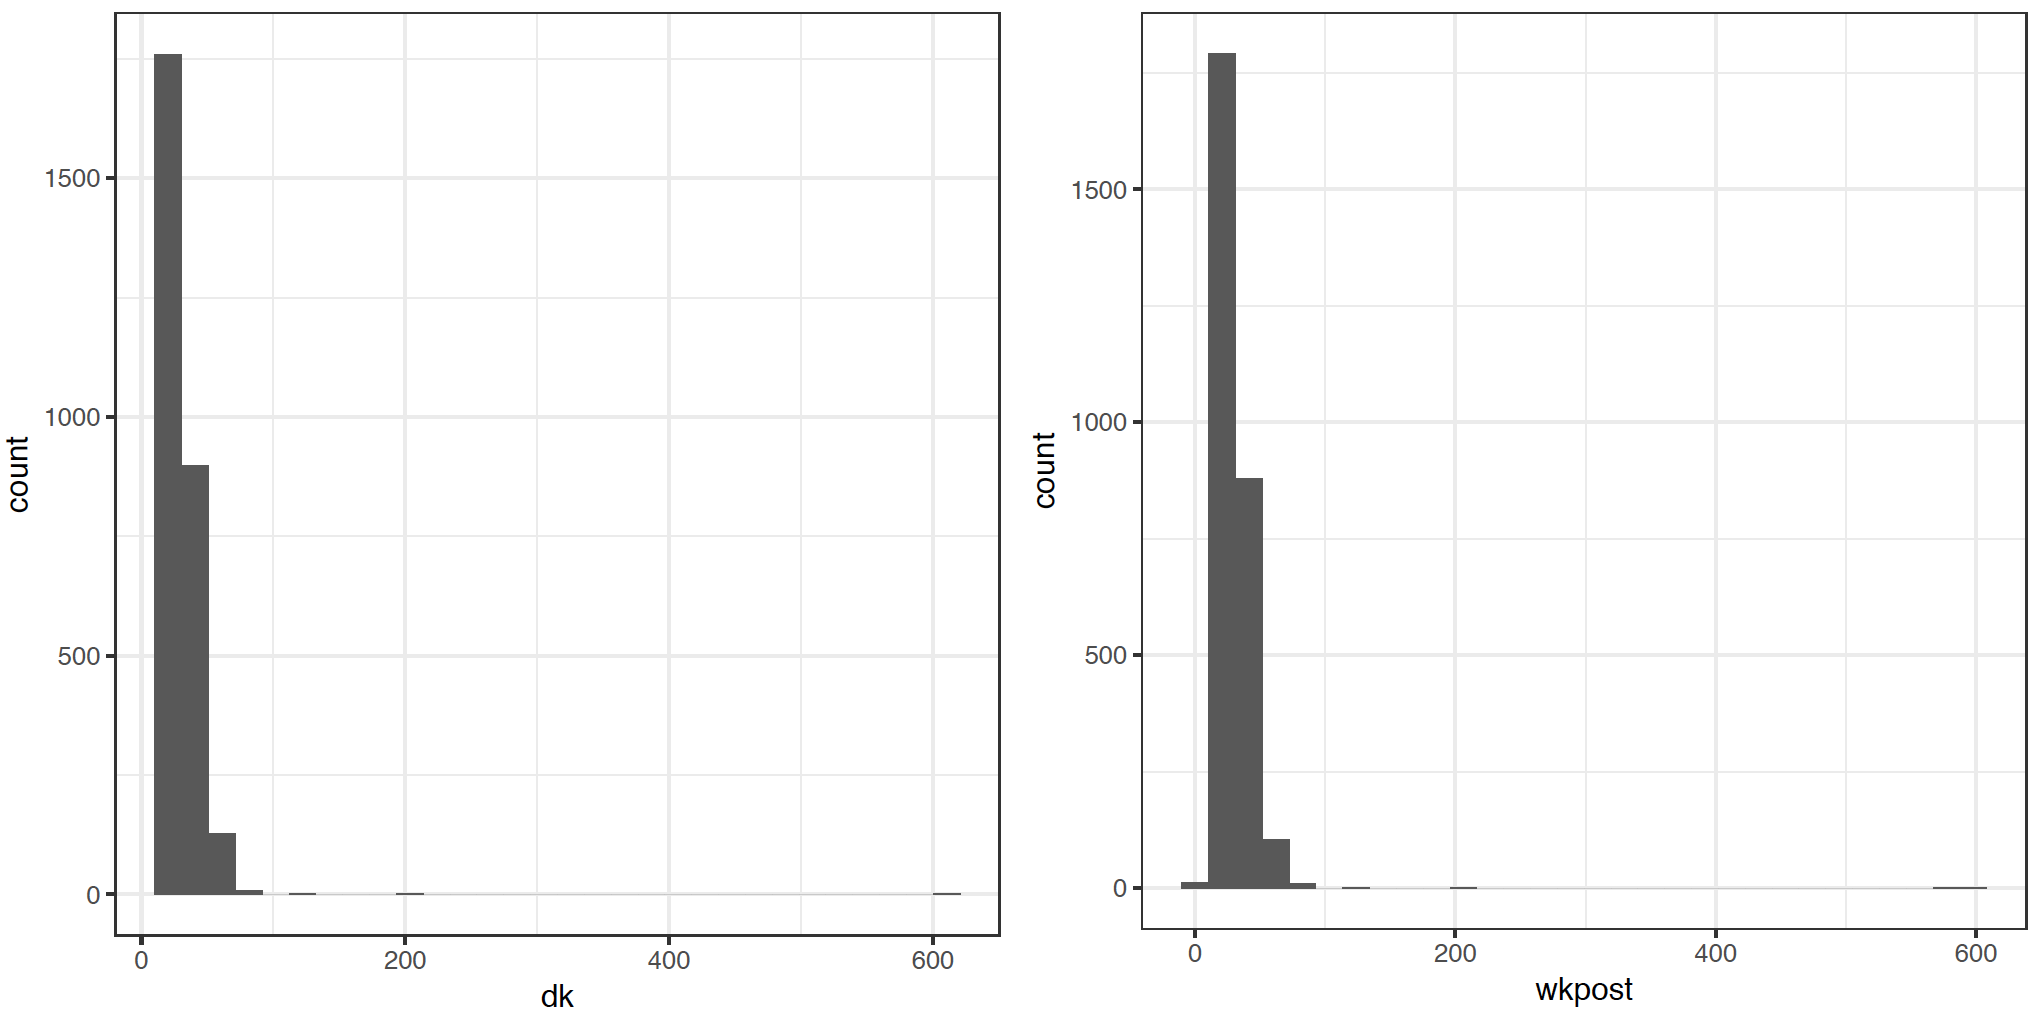
\includegraphics[width=\textwidth,height=5.20833in]{Pics/18.png}
\caption{\emph{Comparación de la distribución de los pesos básicos de muestreo (izquierda) con los pesos ajustados por ausencia de respuesta (derecha) en una encuesta de hogares.}}
\end{figure}

Es posible aumentar la eficiencia del estimar si se crean categorías homogéneas de individuos que tengan la misma probabilidad de responder. En este caso, los valores de las covariables pueden ser usados para crear estas categorías. Por consiguiente, siempre es necesario obtener un conjunto de covariables que esté disponible para respondientes y no respondientes a la vez.

Por ejemplo, en un escenario simplificado, es posible identificar variables como ubicación, edad, sexo, raza, etc. que estén relacionadas con la probabilidad de responder o con la variable de interés (o con ambas). En este caso, se formarían \(Q\) \((q = 1, \ldots, Q)\) categorías de acuerdo al cruce de estas variables para obtener una estimación de la probabilidad de respuesta en cada categoría y ajustar el peso de muestreo. De esta manera, siendo \(s_{q}\) la muestra seleccionada en la categoría \(q\) y \(s_r\) el conjunto de respondientes efectivos, la probabilidad de respuesta en esta categoría se estimaría como:

\[
\phi_{q} = \frac{\sum_{s_{r}\cap s_q}d_{3k}}{\sum_{s_{q}}d_{3k}}
\]

El nuevo peso ajustado por la ausencia de respuesta estará dado por:

\[
d_{4k} = d_{3k}\frac{1}{\phi_{q}} 
= d_{3k}\frac{\sum_{s_q}d_{3k}}{\sum_{s_{r}\cap s_q}d_{3k}}
\]

En un escenario más complejo, si las probabilidades de respuesta fueron estimadas con un modelo de \emph{propensity score} y, teniendo en cuenta que las predicciones de estas probabilidades varían entre cero y uno, es posible crear clases de individuos (respondientes y no respondientes) con probabilidades similares. En este caso, se asumiría que las unidades dentro de una misma clase tendrán la misma configuración de covariables, o al menos, una probabilidad de respuesta estimada similar \(\hat\phi_k\). Así, dentro de cada clase, las unidades serían tratadas como si fuesen sido aleatorizadas al tratamiento (responder) o al control (no responder).

Por lo tanto, el objetivo de este proceso es asegurar que cualquier diferencia en las covariables (edad, raza, etnia, estrato socioeconómico, etc.) pueda ser ajustada. Teniendo en cuenta que, si el modelo es adecuado, la estimación \(\hat\phi_k\) resumiría los efectos de las covariables en la respuesta del individuo, entonces una vez hayan sido creadas las clases es posible realizar el ajuste mediante alguna medida de localización en cada clase y, de esta forma, todos los individuos de una misma clase se ajustarían de la misma manera. \citet{Valliant_Dever_2017} muestran algunas medidas comunmente adoptadas:

\begin{enumerate}
\def\labelenumi{\arabic{enumi}.}
\tightlist
\item
  Promedio no ponderado:
  \[\hat{\phi}_c = \frac{\sum_{k \in s_c}\hat{\phi}_k(\mathbf{z})}{n_c}\]
\item
  Promedio ponderado:
  \[\hat{\phi}_c = \frac{\sum_{k \in s_c}d_{2k}\hat{\phi}_k(\mathbf{z})}{n_c}\]
\item
  Tasa de repuesta no ponderada:
  \[\hat{\phi}_c = \frac{n_{cr}}{n_c}\]
\item
  Tasa estimada de repuesta:
  \[\hat{\phi}_c = \frac{\sum_{s_c \cap s_r}d_{2k}}{\sum_{s_c}d_{2k}}\]
\item
  Mediana no ponderada:
  \[\hat{\phi}_c = \rm mediana[\hat{\phi}_k(\mathbf{z})]_{k \in s_c}\]
\end{enumerate}

Nótese que, si todas las unidades dentro de una clase tienen la misma probabilidad de responder, entonces la tasa de repuesta no ponderada es la mejor opción. Además, si dentro de las clases las unidades tienen una probabilidad de responder muy disimil, entonces el promedio no ponderado (o ponderado) del PS puede usarse. De la misma manera, la tasa estimada de repuesta puede ser ineficiente si los pesos de muestreo varían demasiado, pero la probabilidad de respuesta es similar en cada clase. Por úlitmo, la mediana se considera si la distribución de la probabilidad de respuesta es sesgada.

\hypertarget{calibraciuxf3n-de-los-pesos}{%
\section{Calibración de los pesos}\label{calibraciuxf3n-de-los-pesos}}

Después de conformar el sistema de ponderación de pesos de muestreo en la encuesta, es posible calibrar estos pesos con la información auxiliar disponible para cada país, a nivel nacional, por estratos de interés, e incluso por variable continuas sobre las que se tenga interés. \citet{Sarndal_Lundstrom_2006} afirman que cuando los estudios por muestreo están afectados por la ausencia de respuesta, es deseable tener las siguientes propiedades en la estructura inferencial que sustenta el muestreo:

\begin{enumerate}
\def\labelenumi{\arabic{enumi}.}
\tightlist
\item
  Sesgo pequeño o nulo.
\item
  Errores estándares pequeños.
\item
  Un sistema de ponderación que reproduzca la información auxiliar disponible\footnote{Por ejemplo, el número de hogares o habitantes en el país.}.
\item
  Un sistema de ponderación que sea eficiente al momento de estimar cualquier característica de interés en un estudio multipropósito.
\end{enumerate}

como se vio en el capítulo anterior, debido a la construcción teórica de los estimadores de calibración, los pesos calibrados responden a la siguiente restricción

\[
\sum_{s}w_{k}\boldsymbol{x}_k = \sum_{U}\boldsymbol{x}_{k} = \boldsymbol{t}_{\boldsymbol{x}}
\]

El ejemplo más básico se encuentra cuando se desea que los pesos de muestreo deberían reproducir con exactitud el tamaño de las regiones \(N_h\) y/o el tamaño del país \(N\). Es así como, utilizar la metodología de calibración \citep{Deville_Sarndal_1992} hace que se cumpla la siguiente ecuación de calibración sobre los nuevos pesos calibrados \(w_k^*\) para todos lo estratos explícitos

\[
\sum_{s_h} w_k = N_h
\]

Esta coherencia entre las cifras oficiales y las que la encuesta puede producir hace que sea preferible el uso de los estimadores de calibración. Las anteriores características son satisfechas al usar el enfoque de calibración que induce una estructura inferencial robusta en presencia de información disponible puesto que reduce tanto el error de muestreo como el error debido a la ausencia de respuesta.

\begin{figure}
\centering
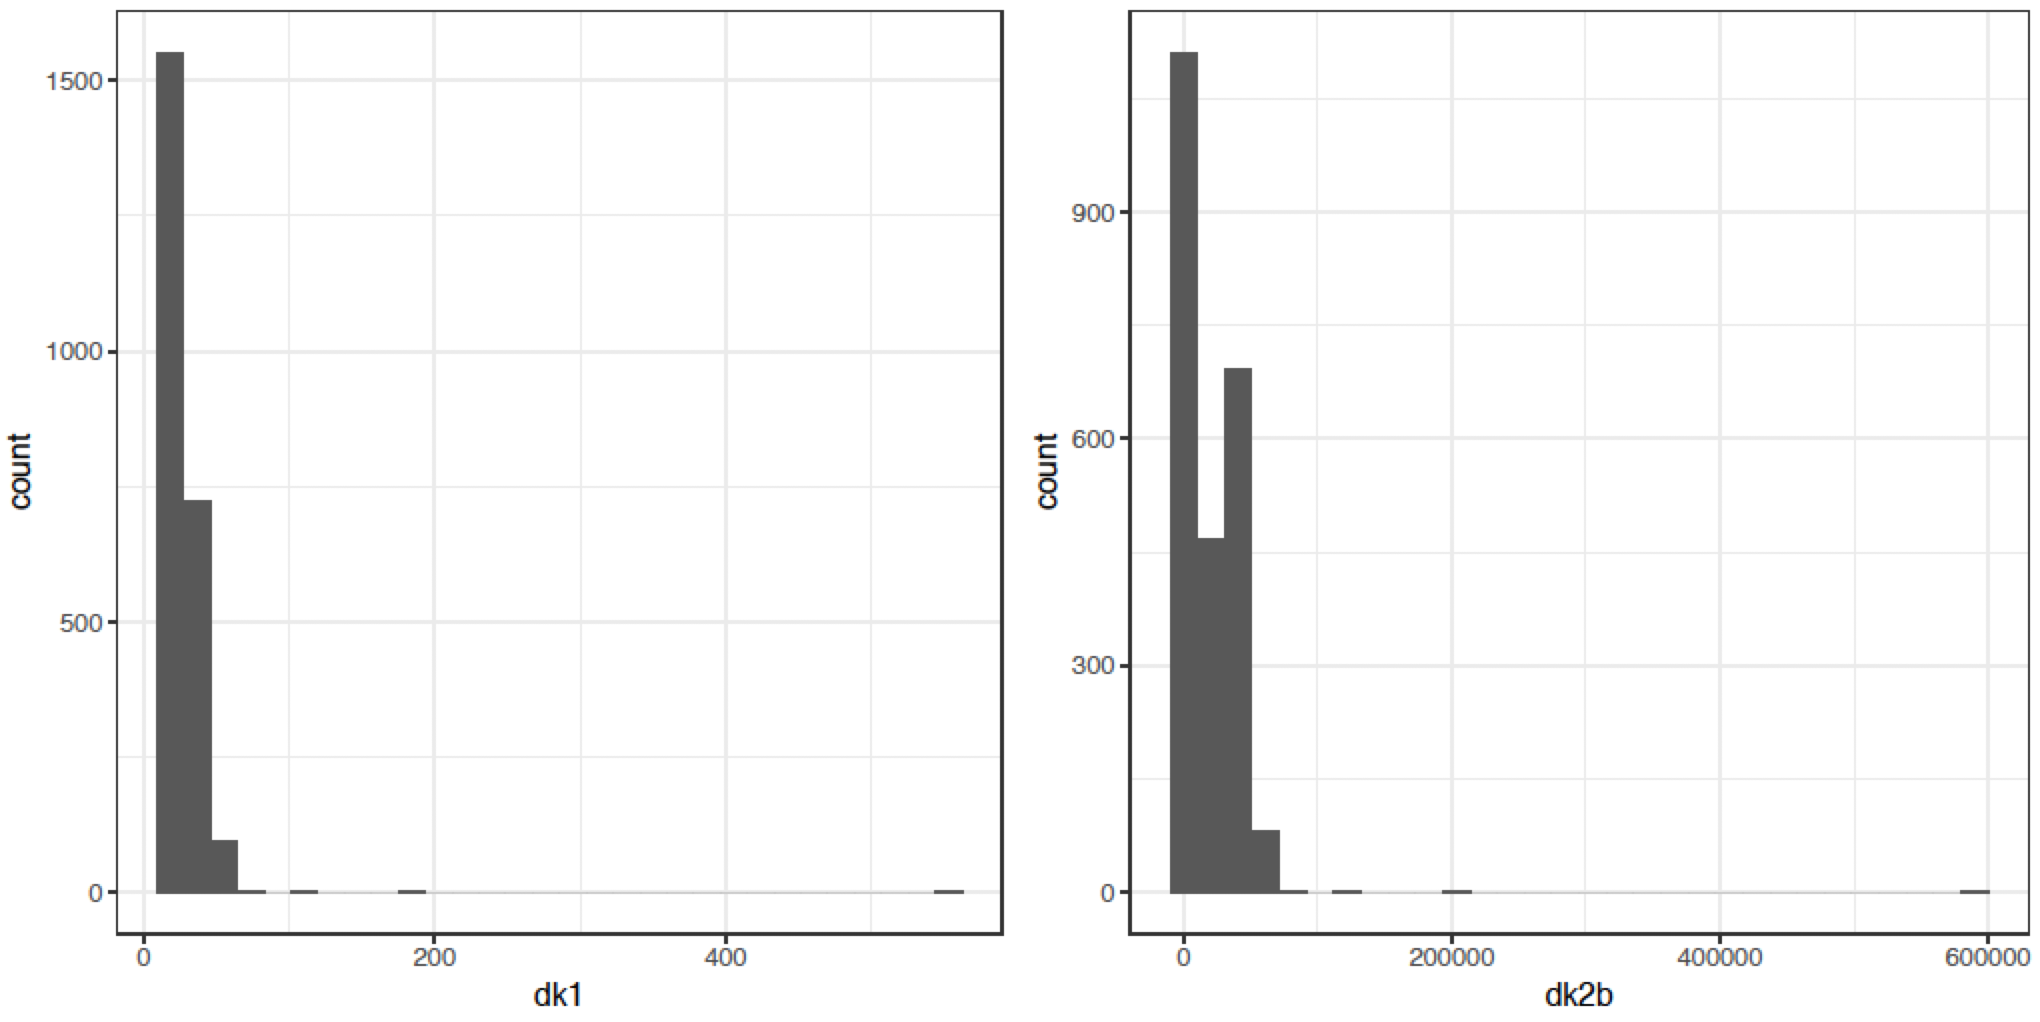
\includegraphics[width=\textwidth,height=5.20833in]{Pics/17.png}
\caption{\emph{Comparación de la distribución de los pesos básicos de muestreo (izquierda) con los pesos ajustados por ausencia de respuesta (derecha) en una encuesta de hogares.}}
\end{figure}

\hypertarget{medidas-de-calidad-en-la-calibraciuxf3n}{%
\subsection{Medidas de calidad en la calibración}\label{medidas-de-calidad-en-la-calibraciuxf3n}}

Los estimadores de calibración son \emph{aproximandamente insesgados}, pero la magnitud del sesgo está dada por la siguiente expresión:

\[
Bias(\hat{t}_{y, cal}) = E_p \left[ \sum_{k \in s} (w_k - d_k) y_k \right]
\]

Si los nuevos pesos calibrados son cercanos a los pesos originales en todas las posibles muestras, entonces el sesgo será insignificante. Ahora, si el tamaño de muestra es insuficiente no conviene utilizar este tipo de estimadores. Además, se sugiere que el coeficiente de variación del estimador de Horvitz-Thompson para las covariables (inducidas por todos los cruces y celdas considerados) sea menor del 10\% para asegurar que el sesgo de los estimadores de calibración sea despreciable.

Por otro lado, cuando se tienen múltiples variables discretas es posible que el cruce de categorías contenga muy pocas unidades para las cuales se deba ajustar los pesos originales. Esto induce sesgo en cada subgrupo ajustado. Si aún así se decide optar por múltiples aumentar las variables de calibración, es necesario hacer un chequeo empírico del ajuste que cada modelo pueda tener con todas las variables de la encuesta, aunque se advierte que este chequeo a veces puede ser demorado e ir en contravía de las apretadas agendas de producción estadísticas que se manejan en el INE.

\citet{Silva_2004} presenta algunas consideraciones al respecto del sesgo que puede generarse al usar esta metodología en las encuestas de hogares y aborda algunos criterios para evaluar la calidad de la calibración. Estas medidas se pueden considerar como protección en contra del sesgo generado por tener demasiadas restricciones. Además, se resalta la importancia de que las variables utilizadas para la calibración sean estimadas de manera precisa por los estimadores clásicos de muestreo. Por ejemplo, si el número de personas en una región es utilizada como una variable de calibración (utilizando como total auxiliar las proyecciones demográficas), entonces el coeficiente de variación del estimador de Horvitz-Thompson sobre esta variable debería ser menor, por ejemplo, al 10\%.

La teoría afirma que entre más variables de calibración se tengan menor será la varianza asociada a las estimaciones (no así el sesgo). Sin embargo, existen problemas computacionales cuando crecen las restricciones que se deben satisfacer son demasiadas. Una primera opción es verificar que no se tengan variables que puedan tener codependencia lineal con otras. Al descartar estas variables es posible conservar una varianza pequeña puesto que se descartan combinaciones lineales de otras variables. Se recomienda hacer un análisis de cuántas variables se deben utilizar en la calibración para optimizar el error cuadrático medio de los estimadores finales en las encuestas de hogares.

En una primera instancia, no sería adecuado utilizar demasiadas restricciones de calibración para satisfacer muchas proyecciones demográficas. Es fácil equivocarse en esta definición. Por ejemplo, si la encuesta es representativa a nivel de departamento (10 niveles), sexo (2 niveles) y edad (4 niveles), entonces sería equivocado utilizar \(10 \times 2 \times 4 = 80\) restricciones de calibración y se debería empezar por analizar una estrategia más parsimoniosa con \(10 + 2 + 4 = 16\) restricciones de calibración. Nótese que a medida que las desagregaciones sean más profundas, el nivel de error en las proyecciones poblacionales será más grande. Ademas, entre más restricciones haya, más sesgo y varianza se introduce a la estimación. La idea general del proceso es encontrar un número de restricciones parsimonioso que permita tener estimaciones aproximadamente insesgadas con una varianza menor a la generada con los factores de expansión originales.

Por otro lado, si los pesos de calibración resultan ser menores que uno su interpretación puede tornarse difícil (aunque no reviste un problema teórico). El usuario común entiende al factor de expansión como un factor de representatividad: \emph{es la cantidad de veces que una persona se representa a sí misma y a algunas otras más en la población}. Por ende, los pesos negativos o menores que uno no resisten esta interpretación intuitiva y natural. Además, los pesos negativos pueden conllevar a estimaciones negativas para algunos dominios en donde el tamaño de muestra es pequeño, lo cual resulta ser problemático en un contexto en donde todas las variables de estudio son no negativas.

Para garantizar que los pesos se ubiquen en un intervalo determinado, se debe minimizar una distancia que a su vez debe inducir pesos restringidos a este intervalo y que respete las ecuaciones de calibración. Es posible que no se tenga una solución exacta para todas las restricciones de calibración e incluso que el algoritmo de calibración no converja. Nótese que los estimadores de calibración se pueden escribir como

\[
w_k = g_k * d_k
\]

Con base en lo anterior, es necesario analizar los pesos \(g_k\) en perspectiva en cada dominio, estrato y postestrato de interés. Una buena idea puede ser identificar aquellos \(g_k\) que resulten potencialmente grandes o influyentes. Se recomienda postestratificar la muestra, y aplicar la calibración a aquellas unidades en los que los \(g_k\) sean estables y usar los pesos originales en el restante conjunto.

Es posible hacer que los pesos de calibración estén restringidos a un espacio predefinido por el usuario, mediante límites \((L, U)\) sobre los \(g_k\). De esta forma, si \(w_k \geq 1\) implica \(g_k \geq 1\) y por tanto \(L=1\). Se acostumbra a tomar \(U > Q_3 + 1.5 * (Q_3 - Q_1)\) en donde \(Q_3\) y \(Q_1\) están dados en términos de la distribución de \(g_k\) y corresponden al tercer y primer cuartil, respectivamente.

Si el mecanismo que genera la ausencia de respuesta no es aleatorio (MAR) o completamente aleatorio (MCAR), es posible que los ponderadores de calibración induzcan sesgo en las estimaciones finales. En general, cuando hay ausencia de respuesta es más probable que aparezcan pesos de calibración negativos y que los pesos de calibración no convergieran a los pesos originales. Además, la varianza de los estimadores de calibración no convergerá a los resultados usuales de los estimadores de regresión.

\citet{Silva_2004} presenta algunas medidas que permiten decidir cuáles escenarios de calibración son los mejores. A continuación se citan tales medidas.

\begin{itemize}
\item
  Error relativo promedio sobre las variables auxiliares
  \[
  M1= \frac{1}{p} \sum_{j=1}^p \frac{|\hat{t}_{xc} - t_x|}{t_x}
  \]
\item
  Coeficiente de variación HT relativo promedio
  \[M2= \frac{1}{p} \sum_{j=1}^p \frac{(Var(\hat{t}_{x\pi}))^{1/2}}{t_x} \]
\item
  Proporción de pesos extremos (límite inferior)
  \[M3 = \frac{1}{n} \sum_{k \in s}I(g_k<L)\]
\item
  Proporción de pesos extremos (límite superior)
  \[M4= \frac{1}{n} \sum_{k \in s}I(g_k>U)\]
\item
  Coeficiente de variación de los \(g_k\)
  \[M5= \frac{\sigma(g)}{\bar{g}}\]
\item
  Distancia entre los pesos de calibración y los pesos originales
  \[M6 = \frac{1}{n}\sum_{k \in s} \frac{(w_k - d_k)^2}{d_k}
  = \frac{1}{n}\sum_{k \in s} d_k(g_k - 1)^2\]
\item
  Eficiencia de los estimadores de calibración sobre la estimación del diseño de muestreo
  \[M7 = \frac{1}{J}\sum_{j=1}^J \frac{Var(\hat{t}_{y_jc})}{Var(\hat{t}_{y_j\pi})} \]
\item
  Efecto de la calibración sobre la dispersión de los ponderadores (DEFFk)
  \[M8 = 1+\frac{\sigma^2_w}{\bar{w}^2}\]
\end{itemize}

\hypertarget{diferentes-niveles-de-calibraciuxf3n}{%
\subsection{Diferentes niveles de calibración}\label{diferentes-niveles-de-calibraciuxf3n}}

Una de las preguntas recurrentes en la calibración de encuestas de hogares es el nivel al cual se debería realizar este ajuste. En principio, es posible realizar la calibración al nivel de las personas, o al nivel de los hogares. Cada una de estas opciones trae algunas ventajas y consideraciones que se deben tener en cuenta.

\begin{itemize}
\item
  Calibrar al nivel de los hogares implica que el hogar tendrá unos nuevos pesos que cumplen con las restricciones de calibración, y esos pesos los heredará a las personas que habitan el hogar. De esta forma todas las personas pertenecientes a un mismo hogar tendrán el mismo peso de muestreo, sin importar sus diferencias en composición demográfica. Por ejemplo, hombres, mujeres, menores y mayores de 15 años tendrán el mismo peso de muestreo. Esta propiedad es atractiva puesto que emula el diseño de muestreo que se definió en la fase de planeación. Sin embargo, realizar la calibración a nivel de los hogares hace que dentro de las unidades primarias de muestreo (UPM) los hogares no tengan un peso homogéneo, lo que se distancia de las propiedades del diseño sistemático simple que se usa para la selección de los hogares dentro de las UPM.
\item
  Por otro lado, calibrar a nivel de personas implica que los pesos de muestreo de los hogares también pueden verse alterados, y que los pesos finales de muestreo de las personas sean diferentes dentro de los hogares. De esta forma, de acuerdo a las características de las personas se tendrá un peso diferente. Por ejemplo, es posible que hombres, mujeres, menores y mayores de 15 años \textbf{no} tengan el mismo peso de muestreo. Por consiguiente cuando se calibra por personas y se utiliza un filtro sobre esa base de personas para crear una base de hogares, las características observadas de los jefes de hogares influenciarían los pesos de muestreo resultantes.
\end{itemize}

Dado que la calibración puede inducir factores de expansión diferentes para los miembros de un mismo hogar, es necesario analizar a qué nivel se realiza este procedimiento (persona, hogar). En principio, y debido al diseño de la encuesta, los pesos de muestreo originales son idénticos para todos los miembros de un mismo hogar. Sin embargo, cuando la post-estratificación trata de ajustar los totales de las restricciones de calibración, y debido a que la población no está equitativamente distribuida, entonces de igual manera se presenta un reajuste en los factores de calibración. Podría ser conveniente revisar la metodología de \emph{raking} y su impacto en los pesos de calibración dentro de los hogares.

Por ejemplo, si la calibración se realiza a nivel de personas y se calibra sobre la población en edad de trabajar, esto traerá como consecuencia que los factores de expansión sean diferentes para los miembros de un mismo hogar, puesto que la metodología buscará ajustar los totales de las personas en edad de trabajar y las personas que no están en la fuerza de trabajo de manera independiente. Por esta razón en la mayoría de hogares, en donde hay personas que son parte de la fuerza de trabajo y personas que no lo son, los pesos de muestreo no serán equivalentes.

\hypertarget{calibraciuxf3n-integrada-en-hogares}{%
\subsection{Calibración integrada en hogares}\label{calibraciuxf3n-integrada-en-hogares}}

En general, la mayoría de encuestas de hogares en la región tienen una naturaleza multipropósito, generando estimaciones de indicadores a nivel de persona (tasa de participación, tasa de desocupación, etc.), y al mismo tiempo, indicadores a nivel de hogar (pobreza monetaria, necesidades básicas insatisfechas y pobreza multidimensional). En este documento se enfatiza la recomendación de disponer de factores de expansión coherentes entre las diferentes unidades de análisis.

Por ejemplo, una práctica común que pone en tela de juicio las propiedades estadísticas del estimador, es generar factores de expansión a nivel de persona y endilgarle el factor de expansión del jefe de hogar al mismo hogar \citep{Alexander_1987}. Esta es una escogencia arbitraria si es que los factores de expansión se han generado mediante una calibración que tenga en cuenta las características de las personas, como por ejemplo edad o sexo. Este acercamiento deliberado no permite sopesar las propiedades estadísticas del estimador resultante y por ende sus resultados no pueden ser interpretados confiablemente, mucho menos comparados.

Una escogencia más parsimoniosa puede ser optar por un enfoque tipo \emph{integrated household weighting}. Nótese que, como lo expone \citet{Heldal_1992}, al realizar una calibración a nivel de personas, ya no será posible agregar a las personas de un mismo hogar para obtener un único peso del hogar, pues las características de las personas del hogar serán, en general, diferentes y sus respectivos factores de expansión también lo serán. Por tanto, es necesario que el sistema de pesos satisfaga la siguiente restricción:

\[
w_j=w_i\ \rm \ para\ toda\ persona\ i\ en\ el\ hogar\ j
\]

De esta forma, si el sistema de pesos de calibración satisface la anterior restricción, sería posible obtener pesos consistentes con las restricciones de calibración a nivel de persona y que permitiera la integración con los hogares, al cambiar de unidad de observación. En la literatura se han descrito varios métodos para lograr esta estandarización.

\hypertarget{agregaciuxf3n-en-los-hogares}{%
\subsubsection*{Agregación en los hogares}\label{agregaciuxf3n-en-los-hogares}}
\addcontentsline{toc}{subsubsection}{Agregación en los hogares}

Es posible realizar el proceso de calibración de factores de expansión sobre la base de datos de las personas o sobre la base de datos de los hogares. De estos dos escenarios calibrar sobre la base de personas parecería ser la opción más rápida puesto que, en la mayoría de los casos, las cifras que se utilizan para calibrar están al nivel de los individuos. Por ejemplo, pensando en una encuesta de fuerza laboral, es evidente que las variables más importantes de la encuesta se encuentran al nivel de las personas y que la calibración de los factores de expansión se debería realizar desde la base de datos de personas.

Por ejemplo, suponga una situación en la cual se desea calibrar por sexo. En este caso, se debería tener acceso a las proyecciones demográficas por sexo para el periodo de referencia de la encuesta y se procedería a calibrar los factores de expansión, utilizando un enfoque de post-estratificación. En este escenario, las ecuaciones de calibración estarían dadas por la siguiente expresión:

\[
\left ( \sum_{k \in s} w_k x_{1k}, \sum_{k \in s} w_k x_{2i} \right )=(t_{x1}, t_{x2})
\]

En donde la suma se hace sobre las personas en la muestra \(s\); además, \(x_{k1}\) toma el valor de uno, si el individuo \(k\) es hombre, y cero en otro caso. Por supuesto, \(x_{k2} = 1 - x_{k1}\), \(t_{x1}\) es la proyección demográfica del total de mujeres y \(t_{x2}\) es la proyección demográfica del total de hombres. En este caso, las covariables de la calibración son variables dicotómicas. Nótese que las ecuaciones de calibración están al nivel de la muestra \(s\) que induce una base de datos de personas. Como el muestreo ha sido en varias etapas, una posibilidad que surge al momento de calibrar los factores de expansión es utilizar la muestra de hogares \(s_I\) que induce una base de datos con información de los hogares y calibrar usando un enfoque de covariables continuas. De esta forma las ecuaciones de calibración estarían dadas por la siguiente expresión:

\[
\left ( \sum_{k \in sI} w_{i} x^h_{1i}, \sum_{k \in sI} w_{i} x^h_{2i}\right )=(t_{x1}, t_{x2})
\]

En donde la suma ahora se realiza sobre los hogares en la muestra de hogares \(s_I\). Nótese que \(x^h_{1i}=(\sum_{k \in sI} w_{i} x^h_{1i})\) se refiere al número de hombres en el hogar \(i\); \(x^h_{2i}=(\sum_{k \in sI} w_{i} x^h_{2i})\) es el número de mujeres en el hogar \(i\); y los totales de calibración \(t_{x1}\) y \(t_{x2}\) siguen siendo el número de hombres y mujeres en la población, respectivamente.

Al respecto, nótese que calibrar con el primer escenario reproduce los totales auxiliares sobre la base de personas, mientras que calibrar sobre el segundo escenario reproduce los totales sobre la base de hogares. Sin embargo, teniendo en cuenta los principios del muestreo en varias etapas y notando que en un hogar, la probabilidad de inclusión de las personas es de uno (inclusión forzosa), entonces generar factores de expansión para las personas en el segundo escenario es muy sencillo puesto que:

\[
w_k=w_i/Pr(k \in U_i | i \in sI) = w_i / 1 = w_i
\]

Es decir que, bajo este escenario de calibración, todas las personas dentro del hogar comparten los mismos pesos de muestreo y además estos pesos son iguales al peso del hogar.

\hypertarget{lemaitre-dufour}{%
\subsubsection*{Lemaitre \& Dufour}\label{lemaitre-dufour}}
\addcontentsline{toc}{subsubsection}{Lemaitre \& Dufour}

El segundo enfoque, condensado en \citet{Lemaitre_Dufour_1987} afirma que se deben crear nuevas variables de calibración a nivel de persona, definidas como el promedio de las variables originales en el hogar. Por ende, se definen las siguientes cantidades:

\[
z_{ij}=\sum_{i\in h} x_{ij}\ \ y\ \ \ {\bar{z}}_{ij}=\frac{z_{ij}}{N_j}
\]

En donde \(z_{ij}\) es la agregación a nivel de hogar de las covariables originales de calibración a nivel de persona y \(N_j\) es el tamaño del hogar \(j\). Al ejecutar el algoritmo de calibración utilizando las variables \(z\), en vez de las variables \(x\), se reproducen las ecuaciones de calibración a satisfacción y, dado que todos los individuos comparten las mismas covariables en la calibración, sus pesos serán idénticos para todos aquellos compartiendo un mismo hogar. Nótese que esta calibración se realiza con la base de datos a nivel de personas.

En segundo lugar, es posible también agregar las covariables de personas a nivel de hogar y ejecutar la calibración con las covariables agregadas. Esta calibración se realiza con la base de datos a nivel de hogares e induce un conjunto de pesos calibrados a nivel de hogar, que fácilmente pueden ser heredados por todos los individuos dentro del hogar. Nótese que, como se trata de una agregación, cuando se cree la base de datos de personas, las ecuaciones de calibración se reproducirán a cabalidad.

En la literatura estadística se ha estudiado este enfoque integrado. Es así como \citet{Neethling_Galpin_2006} concluyeron que, para ambos enfoques, las estimaciones resultantes redujeron el sesgo, aumentaron la precisión y proporcionaron un único conjunto de ponderaciones para los datos de las encuestas estudiadas.

Además, si se opta por el primer enfoque, en el cual el tamaño de la base de datos sería igual al número de personas entrevistadas, se tendría el suficiente margen para actualizar las restricciones de calibración con el fin de ejercer un mayor control sobre los tamaños de los subgrupos de interés.

\hypertarget{estevao-sarndal}{%
\subsubsection*{Estevao \& Sarndal}\label{estevao-sarndal}}
\addcontentsline{toc}{subsubsection}{Estevao \& Sarndal}

En el caso particular en el que haya información auxiliar disponible a nivel de personas y hogares (al mismo tiempo), es posible calibrar conjuntamente ambas variables en un sólo procedimiento de calibración. \citet[sec.~5]{Estevao_Sarndal_2006} recrea la calibración conjunta para hogares y personas, en donde se genera una variable indicadora para el jefe de hogar y sobre esta se crea una nueva restricción de calibración que utilice los totales auxiliares de los hogares. Con esta nueva calibración, se generan unos nuevos pesos de calibración en la base de datos de personas. Al filtrar esta base de datos por el jefe de hogar, se crea inmediatamente una base de hogares (puesto que solo hay un único jefe de hogar) que puede ser utilizada para combinarla con la información de los hogares. De esta forma, los pesos que venían de la base de datos de personas serán los que se utilicen en la base de datos de hogares obteniendo estimaciones consistentes.

En principio, se supone que se selecciona una muestra de unidades de una población finita \(U = \lbrace 1,2,\ldots,k,\ldots,M\rbrace\) la cual está agrupada en conglomerados \(U_I = \lbrace 1, 2,\ldots, i, \ldots, N_I \rbrace\). El proceso de selección se puede resumir de la siguiente manera \citep{Gutierrez_2016}:

\begin{itemize}
\tightlist
\item
  Se selecciona una muestra \(S_I\) de conglomerados de \(U_I\) con probabilidades de inclusión \(\pi_{I_i}\) para \(i\in U_I\). Los pesos muestrales de la primera etapa son \(d_{I_i} = \frac{1}{\pi_{I_i}}\)
\item
  En la segunda etapa se seleccionan unidades para \(i\in S_I\). Se enumeran las unidades en \(U_i\) y se selecciona una muestra \(S_i\) con probabilidades de inclusión condicionales \(\pi_{k|i}\).
\item
  De esta forma, \(d_{k|i} = \frac{1}{\pi_{k|i}}\) son los pesos condicionales y \(d_k = d_{I_i}d_{k|i}\) es el peso de muestreo general para la k-ésima unidad, siendo \(s =\bigcup_{i\in s_I}S_i\) la muestra de unidades.
\end{itemize}

Para calibrar sobre la información auxiliar a nivel de hogar, se deben satisfacer las siguientes ecuaciones:

\[
\sum_{i \in S_I}w_{I_i}x_{ci} = \sum_{i \in U_I}x_{ci} = t_{x_c}
\]

En donde \(x_{ci}\) denota el vector de variables auxiliares a nivel del hogar, que siempre será definido como un conteo de individuos con cierta característica en el hogar. Por ejemplo, en su caso más básico \(x_{ci}\) puede ser el número de individuos en el hogar, mientras que el total auxiliar \(t_{x_c} = \sum_{i \in U_I}x_{ci}\) será el número de individuos en todos los hogares del país. Luego de que se ha calibrado la base de hogares, se construyen los pesos a nivel de persona recurriendo a la siguiente expresión:

\[
w_k = d_{k|i}w_{I_i} \quad \forall k \in S_i
\]

Y además, se preserva la siguiente propiedad
\[
\frac{w_k}{w_{I_i}}=d_{k|i}
\]

Lo anterior imita la propiedad del muestreo en dos etapas de que

\[
\frac{d_k}{d_{I_i}}=d_{k|i}
\]

Como todos los individuos pertenecientes a un hogar son seleccionados para que respondan la encuesta de hogares, se tiene que \(d_{k|i} = 1\), por definición. Por lo tanto, el peso del individuo (en la base de datos de la muestra de personas) será idéntico al peso calibrado del hogar; es decir \(w_k = w_{I_i} \quad \forall k \in S_i\). Por lo anterior, dado que el muestreo es de conglomerados en la última etapa y todos los individuos del hogar son seleccionados, entonces el peso de muestreo del hogar será el promedio de los pesos individuales.

\[
w_{I_i}=\sum_{k\in S_i}\frac{w_k}{N_i}=\sum_{k\in U_i}\frac{w_k}{N_i}=\bar{w}_i
\]

Por último, nótese que la matriz de calibración toma la siguiente forma:

\[
X_{[i]}=X=
\begin{bmatrix}
x_{c11} & x_{c12} & \cdots & x_{c1p}\\
x_{c21} & x_{c22} & \cdots & x_{c2p}\\
x_{c31} & x_{c32} & \cdots & x_{c3p}\\
\vdots  & \vdots & \ddots &\\
x_{cN_I1} & x_{cN_I2} & \cdots & x_{cN_Ip}
\end{bmatrix}
\]

\hypertarget{recorte-de-los-pesos}{%
\section{Recorte de los pesos}\label{recorte-de-los-pesos}}

Un inconveniente que se genera debido a la multitud de ajustes en los factores de expansión es que, si bien el estimador resultante tendrá un sesgo cercano a cero, la distribución de los pesos puede mostrar datos extremos, sobre todo a la derecha de la distribución (valores muy grandes), que hacen que la varianza del estimador crezca y que, por ende, la precisión de la inferencia decrezca. Para hacerle frente a este problema, es posible considerar un procedimiento de \emph{trimming} o recorte de pesos, siguiendo las recomendaciones de \citet[sec.~14.4]{Valliant_Dever_Kreuter_2018}, que puede ser resumido de la siguiente manera:

\begin{enumerate}
\def\labelenumi{\arabic{enumi}.}
\tightlist
\item
  Recortar cualquier peso mayor a un umbral prestablecido en la distribución de pesos ajustados. Por lo general este umbral se fija alrededro de 3.5 veces la mediana de los pesos. Por tanto,
  \[
  U=3.5\times mediana(\mathbf{d_{4k}})
  \]
\item
  Cualquier peso con magnitud superior a \(U\) se trunca de la siguiente manera
  \[
  d_k^\ast=\left\{\begin{matrix}U,\ si\ d_k^\ast\geq U\\
  d_{4k},\ en\ otro\ caso\\\end{matrix}\right.
  \]
\item
  Determinar la cantidad neta perdida debido al recorte de pesos extremos, siguiendo la siguiente expresión:
  \[
  K=\sum_{s_r}(d_k^\ast - d_{4k})
  \]
\item
  Distribuir \(K\) equitativamente entre las unidades que no fueron recortadas.
\item
  Iterar hasta que todos los nuevos pesos calibrados estén por debajo del umbral \(U\).
\end{enumerate}

Al final del proceso se debe asegurar que los datos extremos en los factores de expansión han sido correctamente manejados y que la distribución general de los pesos no sufrió cambios estructurales en los subgrupos poblacionales de interés.

\hypertarget{redondeo-de-los-factores-de-expansiuxf3n}{%
\section{Redondeo de los factores de expansión}\label{redondeo-de-los-factores-de-expansiuxf3n}}

El principio de representatividad es el paradigma inferencial dominante en cualquier encuesta de hogares y el factor de expansión es el concepto más importante en este contexto. Por ejemplo, un hogar en una encuesta con un factor de expansión de 500 se representa a sí mismo y a otros 499 hogares más. La definición teórica del factor de expansión, inducida por el inverso multiplicativo de la probabilidad de inclusión de un hogar en la muestra, hace que la inferencia sea insesgada y confiable. Sin embargo, debido a que la probabilidad de inclusión es un número real contenido en el intervalo \((0, 1]\), entonces su inverso multiplicativo también será un número real mayor que uno.

Cuando el factor de expansión no es entero, entonces su interpretación se torna compleja desde el punto de vista práctico, aunque teóricamente no tenga ninguna repercusión negativa. Sin embargo, este inconveniente puede hacer que, en la práctica, las oficinas nacionales de estadística y los usuarios de las bases de datos de encuestas de hogares tomen la decisión (bienintencionada pero errada) de redondear estas cantidades al entero más cercano. Esta práctica es perjudicial porque le añade sesgo a la inferencia y causará problemas de sobre o sub estimación en algunos dominios de estudio. \citet{Sartore_Toppin_Young_Spiegelman_2019} plantean que el redondeo de los factores de expansión puede ser problemático puesto que las estimaciones ponderadas pueden crecer o decrecer enormemente.

Los siguientes ejemplos prácticos muestran de forma directa las repercusiones perjudiciales que conlleva esta práctica y que son consecuencia directa del sesgo de redondeo:

\begin{enumerate}
\def\labelenumi{\arabic{enumi}.}
\tightlist
\item
  En encuestas de establecimientos redondear el factor de expansión en las unidades que tienen flujos de ventas grandes trae problemas de sesgo en este dominio de estudio.
\item
  En encuestas agropecuarias, si una unidad productiva produce un cuarto de la producción nacional, el redondeo de su factor de expansión es nefasto.
\item
  En encuestas de hogares, en donde los diseños de muestreo son generalmente auto-ponderados (en donde todas las viviendas comparten el mismo factor de expansión) dentro de los estratos, redondear el factor de expansión implica sesgar por completo todo el estrato.
\end{enumerate}

Suponiendo que una muestra probabilística \(s=(I_1,\ldots,I_k,\ldots,I_N)'\) fue seleccionada de una población finita \(U\) mediante un diseño de muestreo que induce probabilidades de inclusión \(\pi_k= E(I_k)\) para todos los individuos \(k \in U\) (en donde \(I_k\) toma el valor uno si fue seleccionado o cero en otro caso) entonces desde el punto de vista teórico los estimadores de muestreo \(\hat t_y = \sum_s d_k \ y_k\) son insesgados cuando el factor de expansión \(d_k\) es idéntico al inverso de la probabilidad de inclusión, puesto que

\[
E(\hat t_y)
= E \left( \sum_s \frac{y_k}{\pi_k} \right)
= E \left(\sum_U I_k \frac{y_k}{\pi_k} \right)
= \sum_U E(I_k)  \frac{y_k}{\pi_k}
= \sum_U \pi_k \frac{y_k}{\pi_k} = t_y
\]

De las anteriores relaciones es evidente que, cuando el factor de expansión se redondea de forma determinística, entonces \(E(\hat t_y) \neq t_y\). Para evadir el sesgo de redondeo, es necesario emplear un método aleatorio que induzca insesgamiento en los estimadores de muestreo. En general, este problema puede ser abordado desde una perspectiva probabilística. De hecho, si en primera instancia se utiliza como redondeo la parte entera (el entero máximo que sea menor o igual) del factor de expansión, entonces bastará con añadir aleatoriamente una unidad a algunos factores de expansión para asegurar que la suma de los factores redondeados sea idéntica a la original. Con esta simple idea se le devuelve la propiedad del insesgamiento a los estimadores de muestreo.

\begin{algorithm}
\DontPrintSemicolon
\KwIn{Factores de expansión originales $d_k$}
\KwOut{Factores de expansión redondeados $\tilde d_k$}
\Begin{
  \For{$k \in s$}{
  $\phi_k = d_k - \lfloor d_k \rfloor$
  }
Seleccionar una submuestra $s_a=(c_1,\ldots,c_k,\ldots,c_n)'$ de $s$ con probabilidades de inclusión $\phi_k$\;
  \eIf{$c_k = 0$} {
    $\tilde d_k = \lfloor d_k \rfloor$\;
    }{
    $\tilde d_k = \lfloor d_k \rfloor + 1$\;
  }
}
\Return{$\tilde d_k$}\;
\end{algorithm}

En primera instancia, nótese que la submuestra \(s_a\) no necesariamente será de tamaño fijo, puesto que \(\sum_s\phi_k\) no será entera en todos los casos; por ende, es posible utilizar un algoritmo de muestreo Poisson \citep[sección 4.1]{Gutierrez_2016} para seleccionar esta submuestra. Sin embargo, si esta suma es entera, es posible utilizar un algoritmo de muestreo más eficiente que induzca una submuestra de tamaño fijo como por ejemplo el método de Brewer. Por otro lado, la esperanza de estos factores redondeados condicionados a la submuestra \(s_a\) es igual a los factores de expansión originales, tal y como se muestra a continuación

\[
E(\tilde d_k | s_a) 
= \lfloor d_k \rfloor + E(c_k|s_a) 
= \lfloor d_k \rfloor + \phi_k
= d_k
\]

Por lo anterior, es importante notar que el uso de este método aleatorio de redondeo siempre induce insesgamiento en los estimadores de muestreo, puesto que

\[
E \left( \sum_s \tilde d_k y_k \right) 
= E E \left( \sum_s \tilde d_k y_k  | s_a\right) 
= E \left( \sum_s E(\tilde d_k | s_a) y_k \right) 
= E \left( \sum_s d_k y_k \right) = t_y
\]

Por último, cuando los factores de expansión de la encuesta están calibrados se presenta un problema de optimización un poco más complejo, puesto que al utilizar el redondeo aleatorio, los factores de expansión perderan la propiedad de calibración. \citet{Sartore_Toppin_Young_Spiegelman_2019} y \citet{Tille} han presentado diferentes soluciones a este problema, siendo la última mucho más fácil de implementar en el software estadístico \texttt{R}. Bajo esta perspectiva, la calibración de los factores de expansión crea nuevos pesos denominados \(w_k\) que conservan la siguiente propiedad para un conjunto de totales auxiliares \(\mathbf{t_x}\) disponibles para toda la población

\[
\sum_s w_k \mathbf{x}_k =  \mathbf{t_x}
\]

El siguiente algoritmo hace uso del muestreo balanceado \citep[capítulo 8]{Tille_2006}, el cual representa una forma de calibración desde el diseño de muestreo y es una solución óptima para seleccionar la submuestra \(s_a\) y por ende preservar la consistencia de los pesos calibrados con los totales auxiliares.

\begin{algorithm}
\DontPrintSemicolon
\KwIn{Factores de expansión calibrados $w_k$}
\KwOut{Factores de expansión redondeados y calibrados $\tilde w_k$}
\Begin{
  \For{$k \in s$}{
  $\phi_k = w_k - \lfloor d_k \rfloor$\;
  $\tilde{\mathbf{x}}_k = \phi_k \ \mathbf{x}_k$
  }
Seleccionar una submuestra balanceada $s_a=(c_1,\ldots,c_k,\ldots,c_n)'$ de $s$ con probabilidad $\phi_k$ tal que 
\begin{equation*}
\sum_{k \in s_a} \frac{\tilde{\mathbf{x}}_k}{\phi_k} 
\cong
\sum_{k \in s} \tilde{\mathbf{x}}_k
\end{equation*}
  \eIf{$c_k = 0$} {
    $\tilde w_k = \lfloor w_k \rfloor$\;
    }{
    $\tilde w_k = \lfloor w_k \rfloor + 1$\;
  }
}
\Return{$\tilde w_k$}\;
\end{algorithm}

Es importante recalcar que la restricción en la submuestra implica que los pesos redondeados cumplan la siguiente relación

\[
\sum_s c_k \ \mathbf{x}_k 
\cong \sum_U \mathbf{x}_k 
- \sum_U \lfloor w_k \rfloor \ \mathbf{x}_k 
\]

Lo cual conlleva inmediatamente a que los nuevos pesos, además de estar redondeados, también estén calibrados; es decir
\[
\sum_s \tilde w_k \mathbf{x}_k \cong  \mathbf{t_x}
\]

Nótese que el redondeo aleatorio depende de la selección de la submuestra \(s_a\) para completar los restos de la parte entera. En esta selección intervienen diferentes algoritmos de muestreo que se pueden aplicar fácilmente utilizando la librería \texttt{sampling} \citep{Matei}. Por ejemplo, suponga una muestra de tamaño \(n= 200\) que fue seleccionada de una población de tamaño \(N=9200\) con factores de expansión desiguales que no están calibrados. Asuma que el vector de probabilidades de inclusión en la muestra toman la siguiente forma

\[
\boldsymbol{\pi}_s = (\underbrace{15/500}_{50 \ veces},
\ldots,
\underbrace{15/800}_{80 \ veces}, 
\ldots,
\underbrace{15/700}_{70 \ veces})'
\]

Por lo tanto, el vector de pesos de muestreo estará definido de la siguiente manera:

\[
\mathbf{d}_s = (\underbrace{33.33333}_{50 \ veces},
\ldots,
\underbrace{53.33333}_{80 \ veces}, 
\ldots,
\underbrace{46.66667}_{70 \ veces})'
\]

De la misma manera, el vector de excesos \(\phi_k = w_k - \lfloor d_k \rfloor\), estará dado por la siguiente expresión:

\[
\boldsymbol{\phi}_s = (\underbrace{0.33333}_{130 \ veces},
\ldots,
\underbrace{0.66667}_{70 \ veces})'
\]

Luego del cálculo de \(\phi_k\), se selecciona la submuestra \(s_a\). En particular, en este caso se utiliza el algoritmo de Brewer, puesto que \(\sum_s\phi_k = 90\) y es entero. Al final del proceso de redondeo aleatorio la suma de los nuevos factores coincidirá con la suma de los factores originales.

Por último, si en una segunda instancia, se considera que los pesos están calibrados mediante tres covariables de calibración que respetan las siguientes restricciones:

\[
\sum_{s} (x_{1k}, x_{2k}, x_{3k})' = (1000, 1000000, 11000000)'
\]

Entonces es posible utilizar el método del cubo, en particular la función \texttt{samplecube} del paquete \texttt{sampling} de \texttt{R}, para que la submuestra esté balanceada y los pesos redondeados sigan las restricciones de calibración bajo una tolerancia predefinida.

\hypertarget{enfrentando-la-ausencia-de-respuesta}{%
\chapter{Enfrentando la ausencia de respuesta}\label{enfrentando-la-ausencia-de-respuesta}}

El problema de la ausencia de respuesta es una faceta normal, aunque no deseable, en el desarrollo de una encuesta. Existe un consenso completo de que la ausencia de respuesta puede perjudicar severamente la calidad de las estadísticas calculadas y publicadas en un estudio por muestreo. \citet{Sarndal_Lundstrom_2006} afirman que la ausencia de respuesta ha sido un tópico de interés en las agencias de estadística que producen cifras oficiales en los últimos años. La atención de la literatura hacia este tópico y sus efectos se ha incrementado considerablemente. En parte, esto se debe a un deseo decreciente del público en general para cooperar y reportar los datos solicitados por los Institutos Nacionales de Estadística.

\citet{Lohr_2019} afirma que la mayoría de encuestas tienen cierta ausencia de respuesta residual, aún después de un diseño cuidadoso y un seguimiento de la ausencia de respuesta y establece que existen varios tipos de mecanismos de ausencia de respuesta.

\begin{enumerate}
\def\labelenumi{\arabic{enumi}.}
\tightlist
\item
  Se define la ausencia de respuesta ignorable cuando la probabilidad de que un individuo responda no depende de la característica de interés. Nótese que el adjetivo ignorable hace referencia a que un modelo puede explicar el mecanismo de ausencia de respuesta y que ésta se puede ignorar después de que el modelo la toma en cuenta.
\item
  Por otra parte, la ausencia de respuesta se dice no ignorable cuando la probabilidad de que un individuo responda depende de la característica de interés. Por ejemplo, si en una encuesta de fuerza laboral, se desea estimar el número de personas empleadas o desempleadas, la ausencia de respuesta es no ignorable cuando depende de la clasificación laboral del individuo.
\end{enumerate}

Además, \citet[capítulo 9]{Lumley_2010} hace un análisis detallado con la ausencia de respuesta individual, en donde existen datos parciales para un respondiente, considerando un enfoque que está basado en el diseño de muestreo al ajustar los pesos muestrales. \citet[capítulo 5]{Fuller} cita algunas técnicas de imputación para el tratamiento de la ausencia de respuesta y conjuga modelos probabilísticos junto con los pesos del diseño de muestreo para mitigar los efectos de este problema. \citet{Sar1} considera un enfoque asistido por modelos, en donde toma conjuntos balanceados para lograr mayor representatividad de las estimaciones. De la misma forma, \citet{Sar2} propone un conjunto de indicadores para juzgar la efectividad de la información auxiliar utilizada para controlar el sesgo generado por la ausencia de respuesta.

\hypertarget{clasificaciuxf3n-de-la-ausencia-de-respuesta}{%
\section{Clasificación de la ausencia de respuesta}\label{clasificaciuxf3n-de-la-ausencia-de-respuesta}}

Por otra parte, \citet{Lund} aclaran que existe una gran cantidad de literatura acerca de la ausencia de respuesta y muchos artículos recientes. Esta literatura examina dos aspectos diferentes pero complementarios en el ejercicio de una encuesta: la prevención de la ausencia de respuesta (antes de que ocurra) y las técnicas de estimación necesarias para tener en cuenta la ausencia de respuesta de manera apropiada en el proceso de inferencia. Esta segunda actividad se conoce con el nombre de ajuste para la ausencia de respuesta. \citet{LR2002} establecen tres tipos de mecanismos de ausencia de respuesta.

\begin{enumerate}
\def\labelenumi{\arabic{enumi}.}
\tightlist
\item
  Ausencia de respuesta completamente aleatoria (MCAR - \emph{missing completely at random}): cuando la probabilidad de que un individuo responda no depende de la característica de interés, ni de alguna otra covariable auxiliar. Por ejemplo, si la ausencia de respuesta en una encuesta laboral, no depende del estado actual de empleo del respondiente, ni de alguna característica auxiliar. De esta forma, la ausencia de respuesta está dispersa de manera uniforme sobre toda la población.
\item
  Ausencia de respuesta aleatoria (MAR - \emph{missing at random}): cuando la probabilidad de que un individuo responda depende de algunas covariables auxiliares, pero no depende de la característica de interés. Por ejemplo, en una encuesta de fuerza laboral, la ausencia de respuesta puede depender del nivel socioeconómico del individuo, pero no depende de su clasificación laboral.
\item
  Ausencia de respuesta no aleatoria (NMAR - \emph{not missing at random}): cuando la ausencia de respuesta depende de la característica de interés. Por ejemplo, en la encuesta de fuerza laboral, es posible que los no respondientes dependan de su clasificación laboral. En este caso puede suceder que los desempleados sean los que sistemáticamente no respondan la encuesta.
\end{enumerate}

\hypertarget{ausencia-de-respuesta-de-registro-y-de-unidad}{%
\subsection{Ausencia de respuesta de registro y de unidad}\label{ausencia-de-respuesta-de-registro-y-de-unidad}}

En general se puede afirmar que existen dos tipos de ausencia de respuesta: la primera, debido a la falta de respuesta de una unidad de observación (ausencia de respuesta de unidad), y la segunda debido a la falta de respuesta de una unidad en algunas variables de interés (ausencia de respuesta por registro). La siguiente figura representa el impacto de estos escenarios en la base de datos inicial.

\begin{figure}
\centering
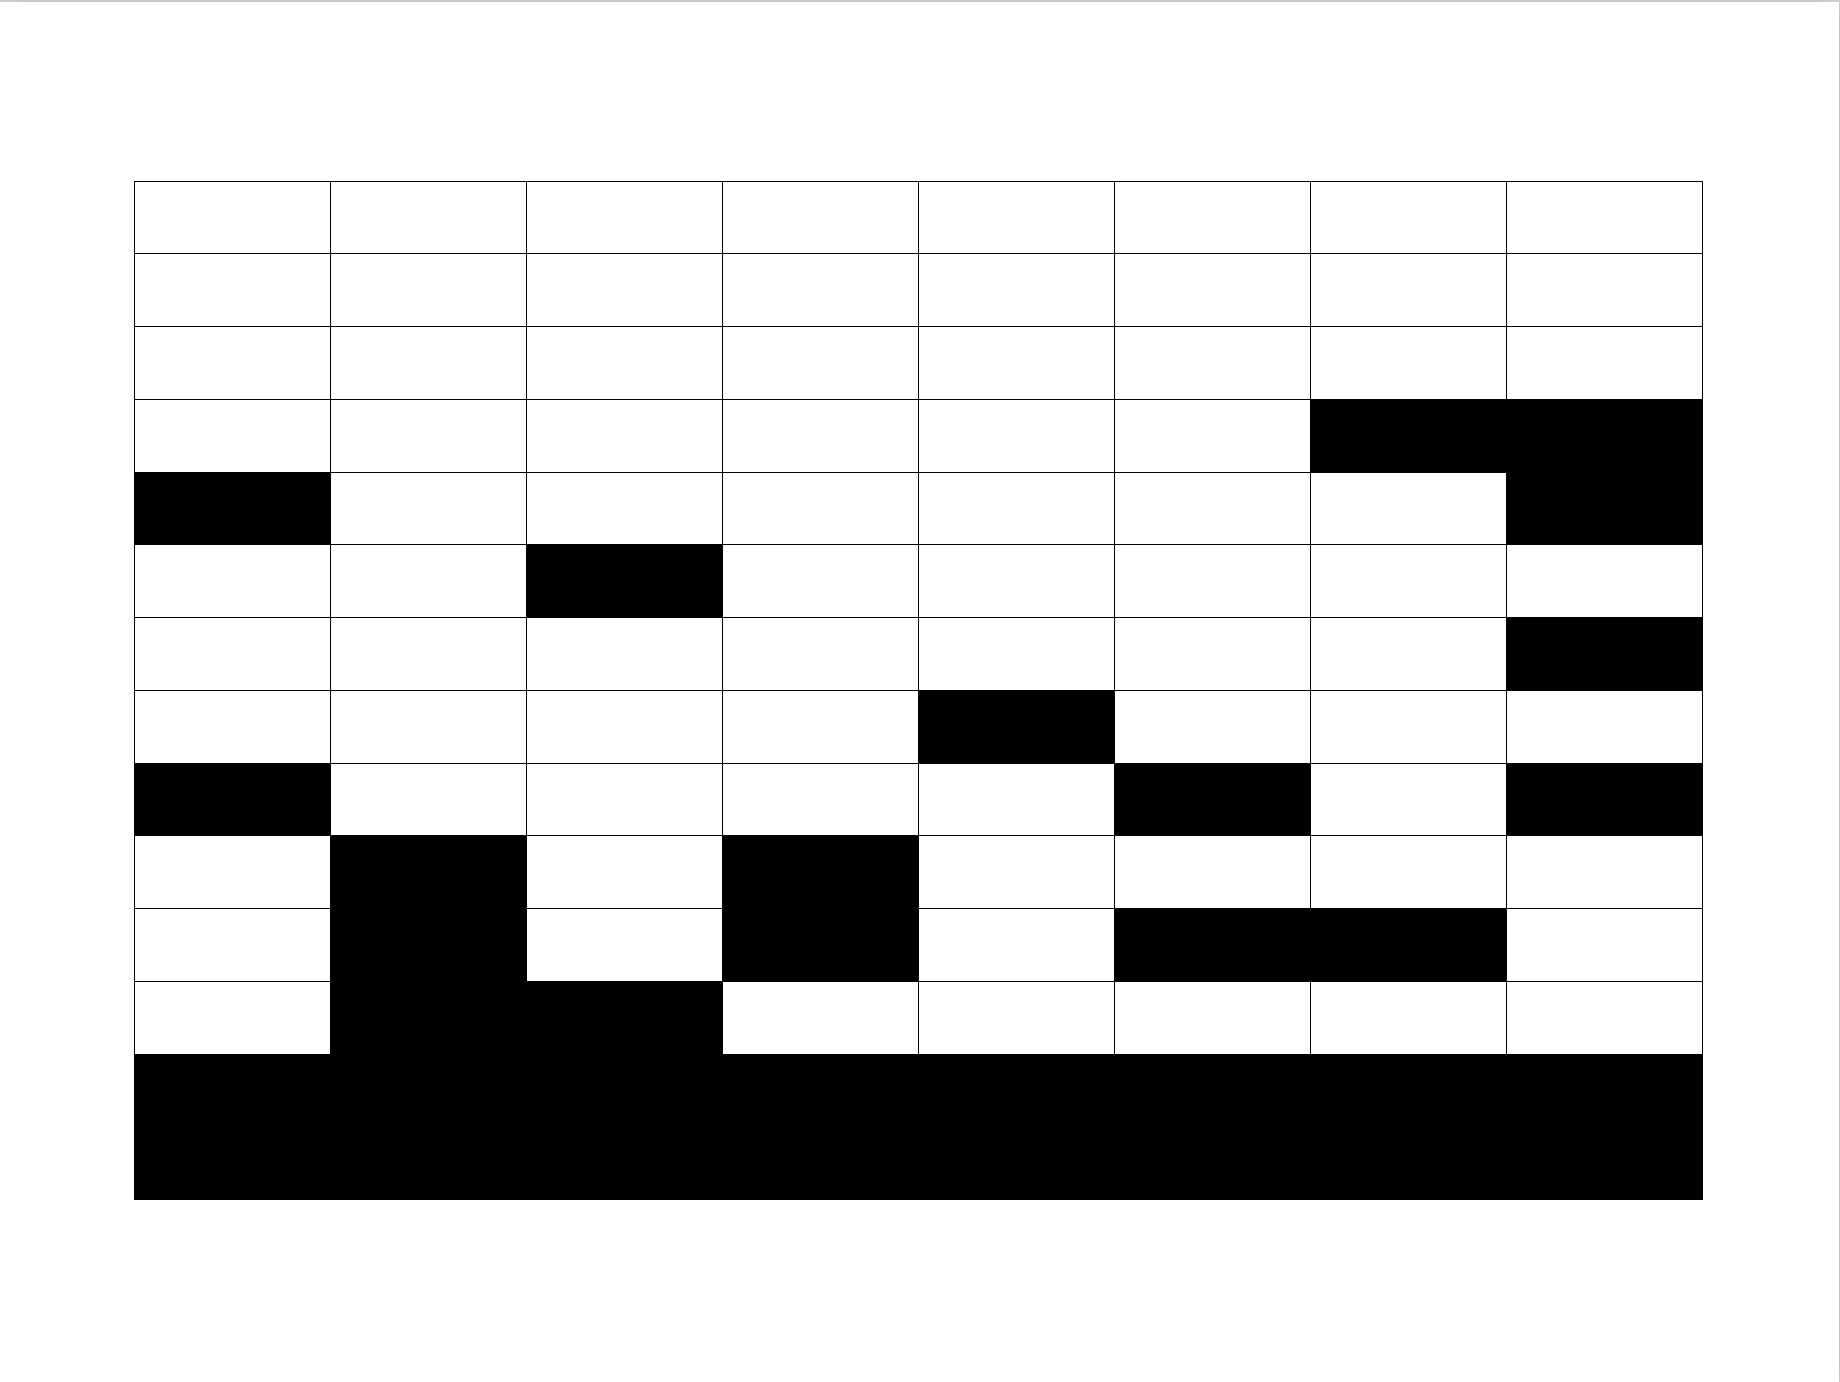
\includegraphics{Pics/nr1.png}
\caption{\emph{Esquema de ausencia de respuesta en una muestra (las celdas en negro representan los valores faltantes en la base de datos).}}
\end{figure}

El primer escenario se evidencia porque en la base de datos inicial falta toda la unidad de observación y sus correspondientes registros. Suele suceder porque el encuestador no pudo establecer contacto con el hogar, o porque la persona seleccionada está enferma o simplemente porque se rehúsa a participar. En esta etapa es recomendable que el encuestador pueda determinar algunas características demográficas del hogar para poder realizar los ajustes pertinentes en el proceso de análisis.

El segundo escenario puede deberse a muchas más causas y se evidencia en la base de datos inicial porque faltan algunos registros de la unidad de observación, aunque otros si están efectivamente respondidos. Suele suceder porque el respondiente se sintió agotado en algún momento del cuestionario, o porque alguna pregunta en particular no fue respondida por considerarse sensible.

\hypertarget{efectos-y-consecuencias-de-la-ausencia-de-respuesta}{%
\subsection{Efectos y consecuencias de la ausencia de respuesta}\label{efectos-y-consecuencias-de-la-ausencia-de-respuesta}}

En general, es posible hacer frente a este fenómeno indeseado desde varias perspectiva. Los siguientes son algunos puntos de vista para enfrentar la ausencia de respuesta:

\begin{enumerate}
\def\labelenumi{\arabic{enumi}.}
\tightlist
\item
  \emph{Ignorancia}: lamentablemente, no es raro que se pretenda ignorar la ausencia de respuesta en la encuesta y realizar inferencias con los datos recopilados de las unidades respondientes, sin realizar ningún tipo de acercamiento estadístico para ajustar la inferencia.
\item
  \emph{Prevención}: diseñar la encuesta de modo que la ausencia de respuesta sea pequeña. Éste es el mejor método de enfrentarla. La capacitación al equipo encuestador, la redacción de las preguntas, la longitud del cuestionario, las revisitas y el agendamiento de las entrevistas pueden palear las altas tasas de asusencia de respuesta.
\item
  \emph{Reacción}: utilizar herramientas para analizar la encuesta de modo que se corrijan los sesgos causados por la ausencia de respuesta. En este caso es posible ajustar los ponderadores de las unidades, o establecer procedimientos de imputación en los registros.
\end{enumerate}

Ignorar la ausencia de respuesta puede tener consecuencias graves en la entendimiento del constructo de interés en la encuesta. Más aún, puede llevar a tomar decisiones erradas de política pública. Por ejemplo, si se omite el efecto de la ausencia de respuesta en una encuesta de ingresos y gastos, se podría subestimar el ingreso medio y el ingreso total en un país; si se omite el efecto de la ausencia de respuesta en una encuesta de desempleo, se podría subestimar el número total de desempleados; además, si se omite el efecto de la ausencia de respuesta en una encuesta de victimización, se podría subestimar el número total de víctimas.

La ausencia de repuesta conlleva grandes efectos de sesgo en los resultados de calidad de las estimaciones. Debe contemplarse muy bien la mejor estrategia para hacer frente a sus consecuencias. Por ejemplo, si se aumentara el tamaño de muestra para enfrentar la ausencia de respuesta, es posible que nos encontremos con una mayor cantidad de personas de la misma clase de respondientes (homogeneidad). En este caso, el sesgo puede aumentar porque se malgastaron recursos que hubiesen servido para remediar la ausencia de respuesta con otras medidas.

\hypertarget{posibles-soluciones}{%
\subsection{Posibles soluciones}\label{posibles-soluciones}}

Al lidiar con la ausencia de respuesta, podemos distinguir algunas prácticas que guían a diferentes tratamientos metodológicos diferentes. En general, se pueden distinguir las siguientes prácticas:

\begin{itemize}
\tightlist
\item
  \textbf{Imputación total}: se trata de imputar todos los valores faltantes para los individuos con al menos un valor perdido. En otras palabras, la imputación se considera como la única forma de tratar la ausencia de respuesta.
\item
  \textbf{Ponderación total}: se trata de ponderar cada una de las variables de interés, así sea de manera diferenciada. No se utiliza la imputación y existirán tantos conjuntos de factores de expansión como variables con valores perdidos.
\item
  \textbf{Eliminación total}: se trata de eliminar todos los registros con algún valor perdido y hacer el análisis con el conjunto restante de valores respondidos.
\item
  \textbf{Enfoque combinado}: se trata de imputar únicamente en los elementos que tienen al menos un registro (no todos) perdido y modificar los factores de expansión en aquellos casos en donde hay omisión de todos los registros del cuestionario.
\end{itemize}

Siguiendo la notación de \citet{Sarndal_Lundstrom_2006}, consideramos una muestra de unidades \(s\), de la cual \(r\) denota el conjunto de respondientes que han contestado a una o más de las \(I\) variables de interés. Por tanto, una unidad que no responde a ninguna variable pertenece al conjunto \(s-r\). El conjunto de unidades que han respondido a una variable del estudio en particular se denota por \(r_i\). Nótese que

\[
r_i\subseteq r \subseteq s
\]

Finalmente, si se supone que \(y_k\) es faltante y se considera para la imputación, entonces \(\hat{y}_k\) denotará su valor imputado

\hypertarget{imputaciuxf3n-total}{%
\subsubsection*{Imputación total}\label{imputaciuxf3n-total}}
\addcontentsline{toc}{subsubsection}{Imputación total}

En este enfoque se imputarían todos los valores \(y_k\) que están perdidos, sin importar si la pérdida es debida a la ausencia del registro o del individuo. En este caso, tendríamos un conjunto completo de datos con los valores \(\{y_{\circ \  k}: k\in s\}\), donde

\[
y_{\circ \  k} = 
\begin{cases}
y_k, \ \text{for $k \in r_i$} \\
\hat{y}_k, \ \text{for $k \in s - r_i$}
\end{cases}
\]

y \(\hat{y}_k\) es el valor imputado. Por ejemplo, el estimador del total utilizando este enfoque estaría dado por la siguiente expresión.

\[
\hat{t}_{y,\pi} = \sum_s d_{k}y_{\circ \  k}
= \sum_{r_i}d_{k}y_k + \sum_{s - r_i}d_{k}\hat{y}_k
\]

Nótese que en el siguiente gráfico, cada valor faltante (que originalmente estaba en color negro en la base de datos) ahora es estimado (en color gris) y participaría en el proceso inferencial con una base de datos completa, pero imputada.

\begin{figure}
\centering
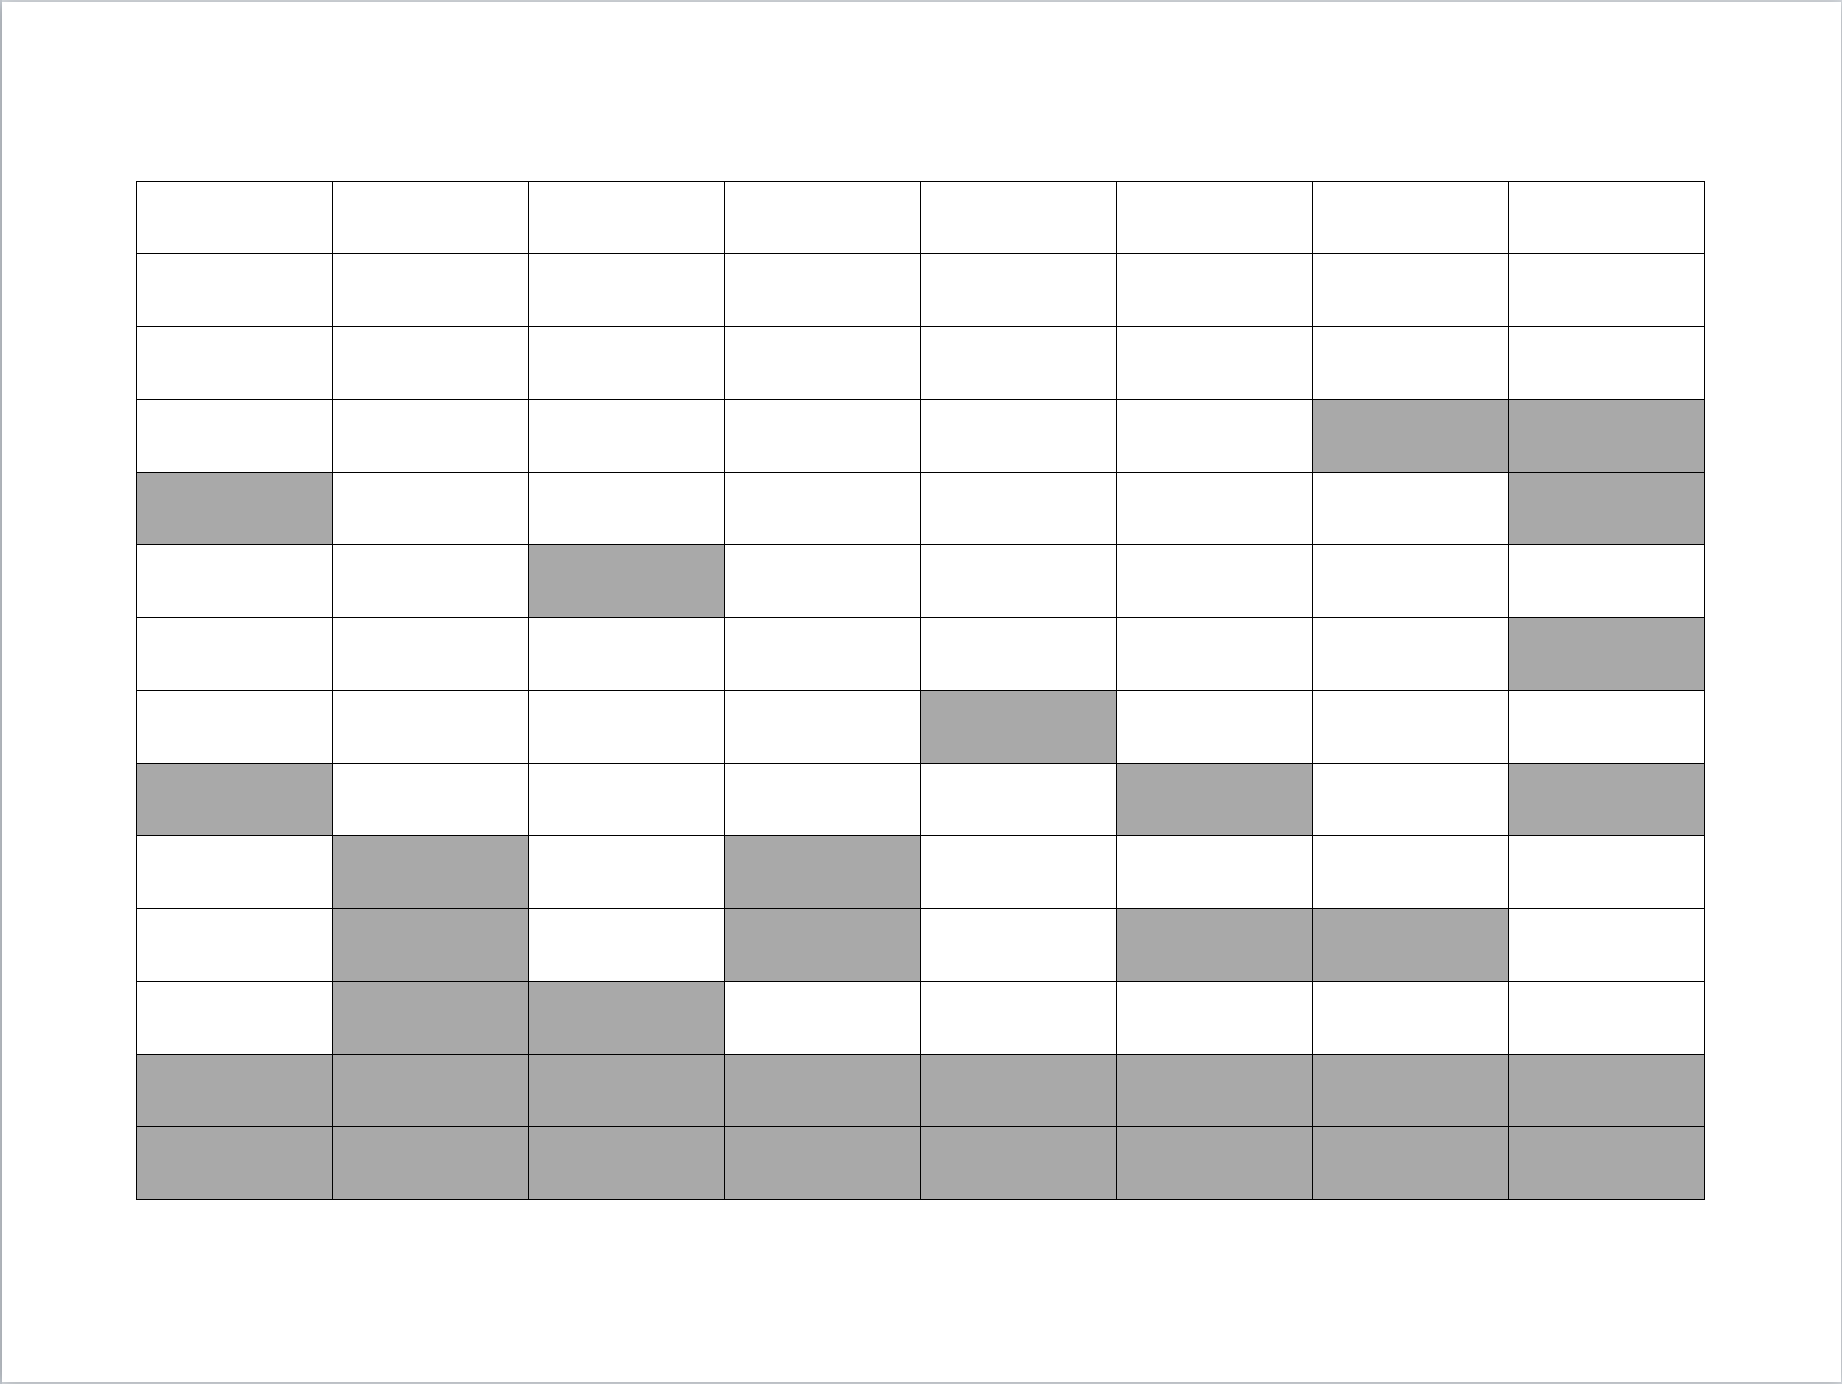
\includegraphics{Pics/nr3.png}
\caption{\emph{Enfoque de inputación total}}
\end{figure}

\hypertarget{ponderaciuxf3n-total}{%
\subsubsection*{Ponderación total}\label{ponderaciuxf3n-total}}
\addcontentsline{toc}{subsubsection}{Ponderación total}

Al usar el enfoque de ponderación total es posible usar pesos de calibración específicos \(w_k = d_k F_{ik}\) que compensarían la ausencia de respuesta de unidad y de registro. De esta forma, el estimador del total estaría dado por la siguiente expresión:

\[
\hat{y}_{cal}=\sum_{r_i}w_ky_k = 
\sum_{r_i}d_k F_{ik} y_k
\]

Si todos los \(r_i\) son diferentes, entonces cada variable de estudio requerirá un conjunto de ponderadores diferentes. Basado en la siguiente gráfica, nótese que este camino elimina, de manera diferencial, todos los registros faltantes de la base de datos original (en color negro). Al final este enfoque induce un número no uniforme de casos por variable.

\begin{figure}
\centering
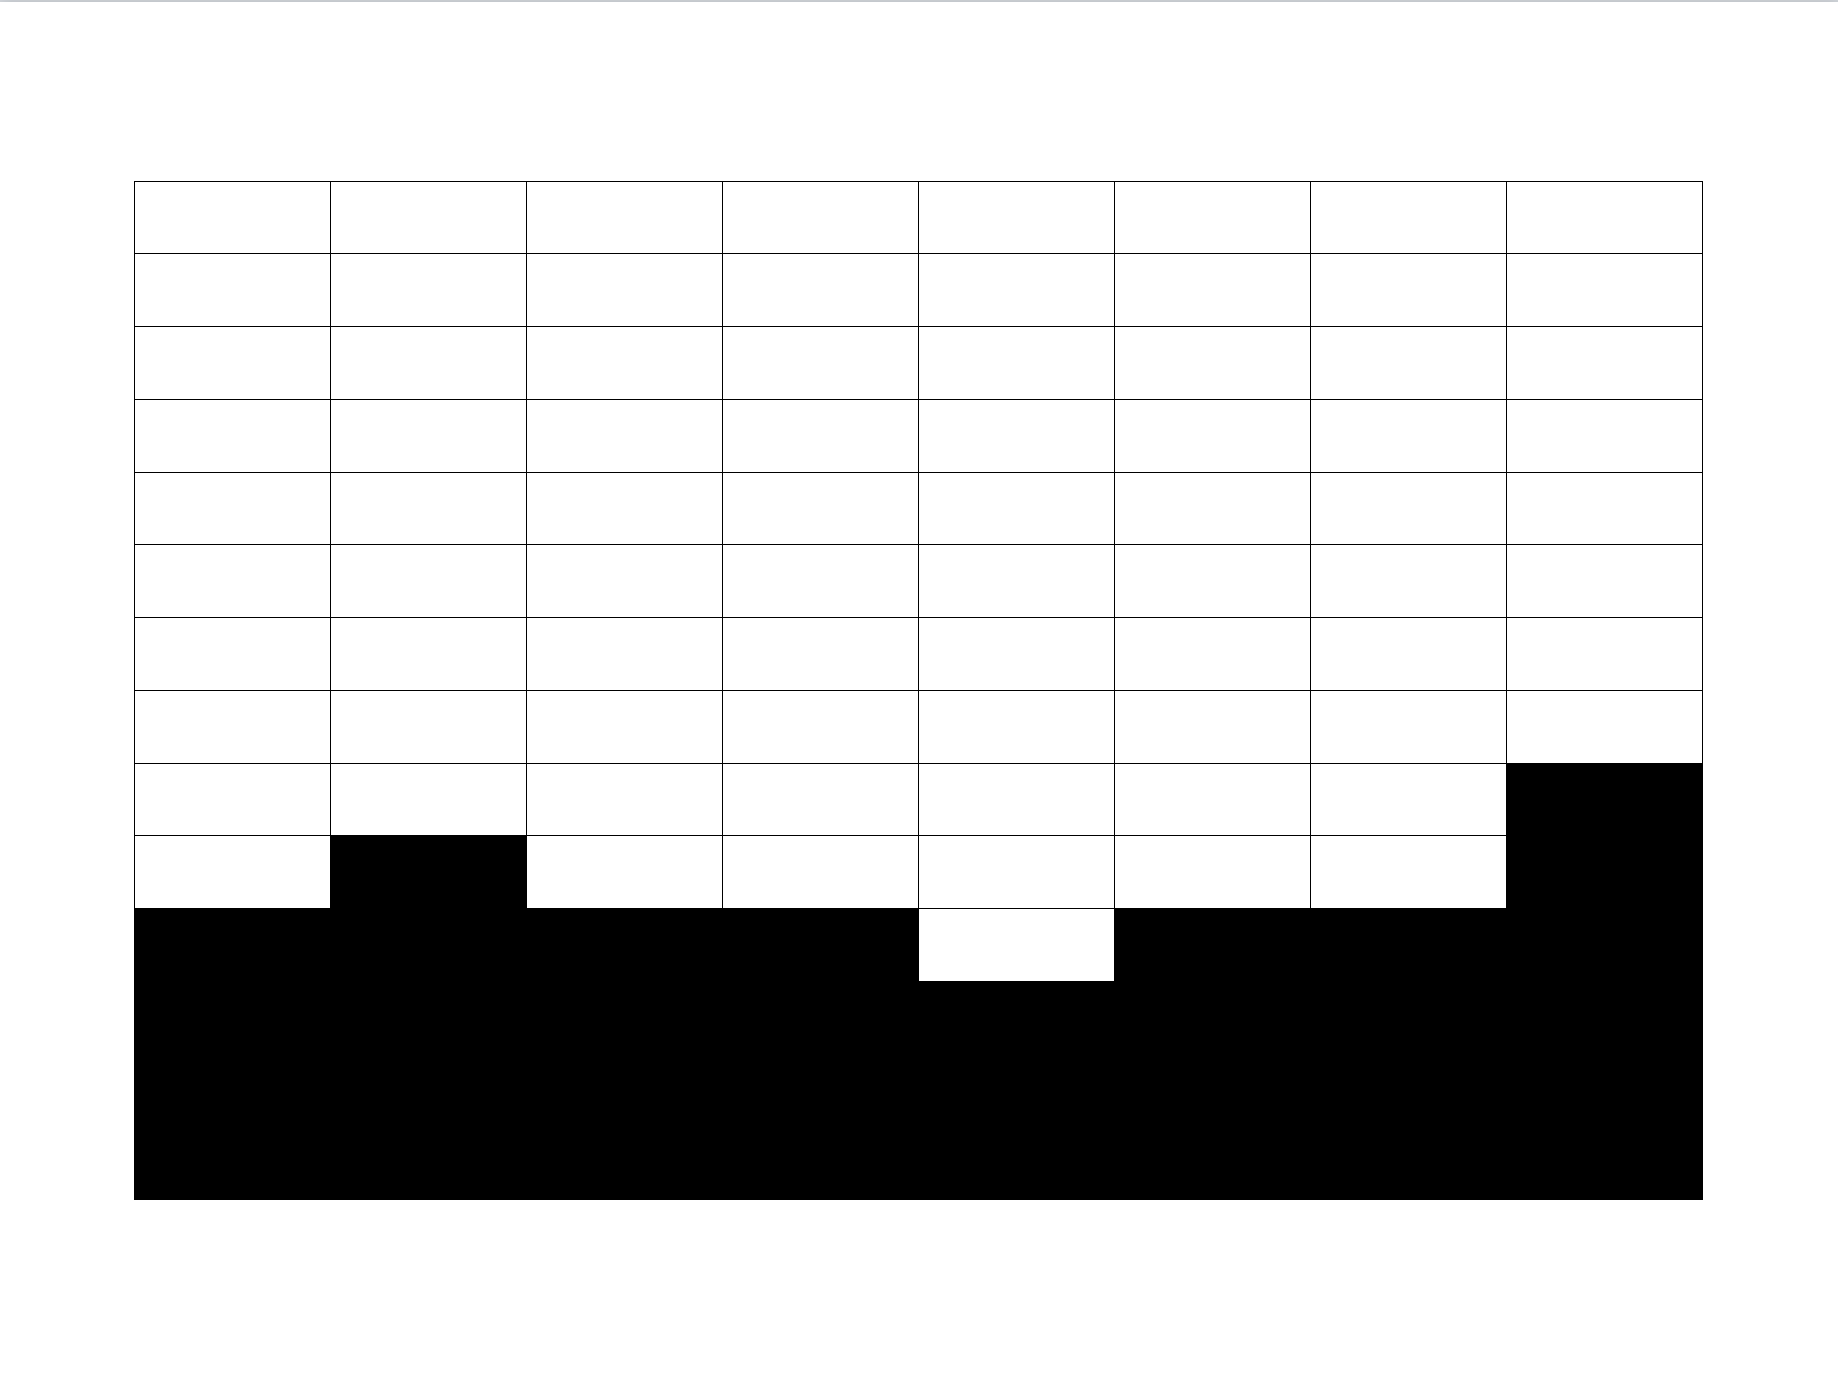
\includegraphics{Pics/nr4.png}
\caption{\emph{Esquema de ausencia de respuesta en una muestra}}
\end{figure}

\hypertarget{eliminaciuxf3n-total}{%
\subsubsection*{Eliminación total}\label{eliminaciuxf3n-total}}
\addcontentsline{toc}{subsubsection}{Eliminación total}

En este enfoque se eliminarán de la base de datos todas las unidades que contengan al menos un registro perdido. En este caso, tendríamos una pérdida considerable del tamaño de muestra, aunque induciría un solo conjunto de ponderadores. Se recomienda fuertemente abstenerse de tomar este camino. La siguiente gráfica representa este enfoque en donde es evidente que el decrecimiento en el tamaño de muestra podría tener repercuciones nefastas en la inferencia de la encuesta.

\includegraphics{Pics/nr2.png}

\hypertarget{enfoque-combinado}{%
\subsubsection*{Enfoque combinado}\label{enfoque-combinado}}
\addcontentsline{toc}{subsubsection}{Enfoque combinado}

Por el contrario, es recomendable escoger un camino parsimonioso que combine estas estrategias de forma diferencial a lo largo de la encuesta. El enfoque combinado usa la imputación para afrontar la ausencia de respuesta por registro para las variables específicas que lo necesiten y luego utiliza un ajuste a los factores de ponderación para afrontar la ausencia de respuesta por unidad. Usualmente, los pesos finales se producen utilizando un enfoque de calibración que hace uso de información auxiliar externa.

Cuando se presenta ausencia de respuesta por registro y por unidad, el enfoque combinado imputa primero para luego obtener una matriz rectangular completa. Luego de lo anterior se procede a realizar un ajuste a los ponderadores. El conjunto de datos completo para la variable de interés \(y\) está dado por \(\{y_{\circ \  k}: k\in r\}\)

\[
y_{\circ \  k} = 
\begin{cases}
y_k, \ \text{for $k \in r_i$} \\
\hat{y}_k, \ \text{for $k \in r - r_i$}
\end{cases}
\]

En donde \(\hat{y}_k\) es el valor imputado. Note que en el enfoque de imputación total, también se imputa para \(k \in s-r\). La siguiente gráfica representa este enfoque parsimonioso en donde los valores imputados (en gris) entran a ser parte de la inferencia y las unidades que nunca respondieron (en negro) y que tienen todos sus registros faltantes son retiradas de la base de datos final.

\begin{figure}
\centering
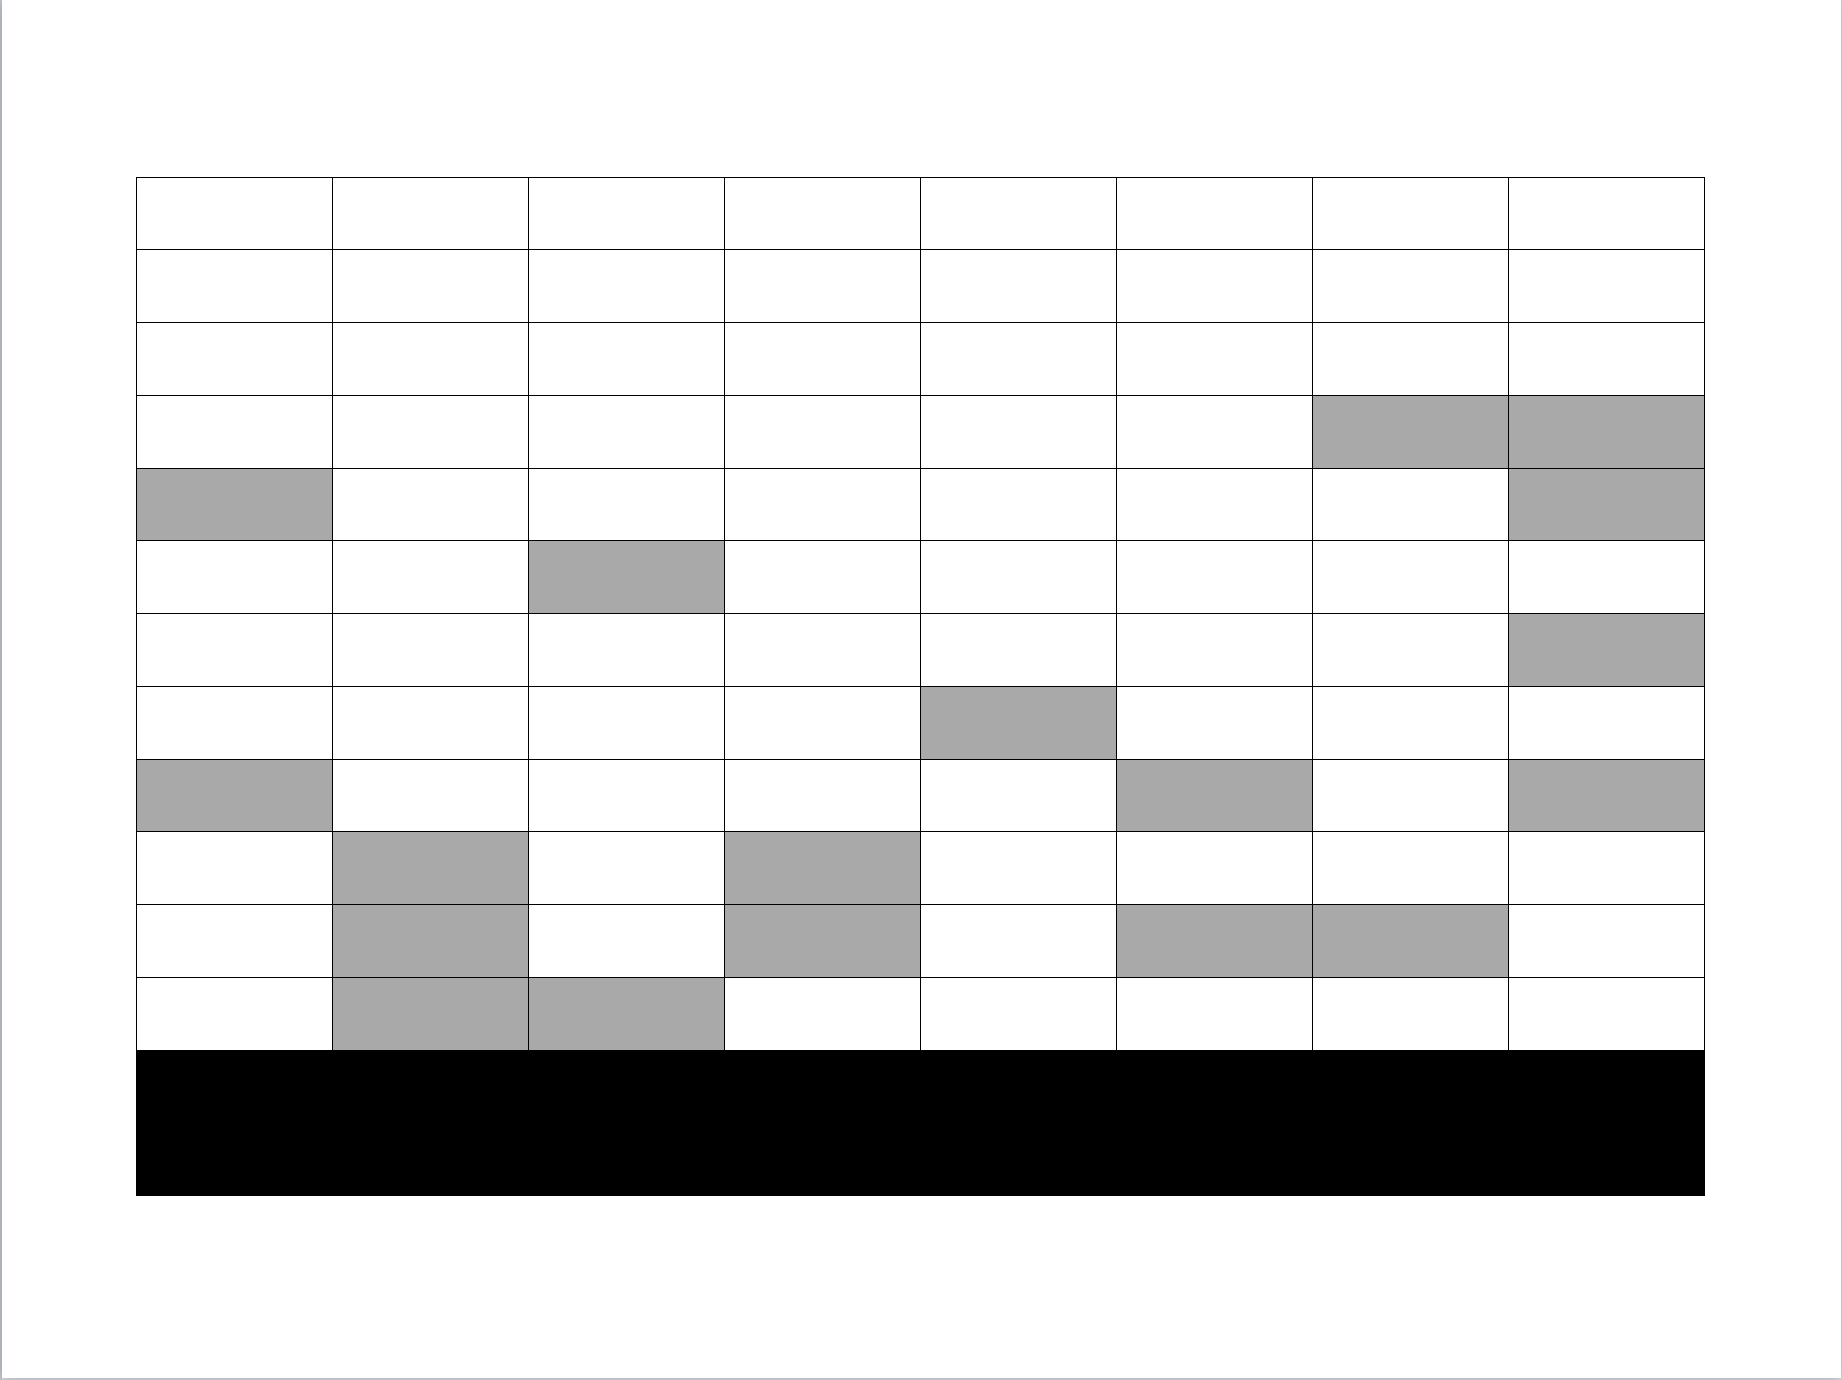
\includegraphics{Pics/nr5.png}
\caption{\emph{Enfoque combinado}}
\end{figure}

\hypertarget{indicadores-de-representatividad}{%
\section{Indicadores de representatividad}\label{indicadores-de-representatividad}}

Como se mencionó anteriormente, la mayoría de las encuestas adolecen de falta de respuesta y este fenómeno puede afectar seriamente la calidad de
los resultados de una encuesta. De hecho, las estimaciones de las características de la población estarán sesgadas si, debido a la falta de respuesta, algunos grupos de la población quedan sobre-representados o sub-representados; el problema se agrava cuando estos grupos
se comportan de manera diferente con respecto a las variables de la
encuesta. En referencia a la ausencia de respuesta de unidad, en general los INE de la región a menudo usan la tasa de respuesta de la encuesta como un indicador de la calidad de la encuesta.

Dado que una tasa de respuesta baja no implica necesariamente que la precisión de las estimaciones de la encuesta sea deficiente, centrarse solo en la tasa de respuesta como indicador de la calidad de la encuesta puede ser engañoso. Por ejemplo, \citet{Bethlehem_Cobben_Schouten_2009} ilustran esta situación con un ejemplo de la encuesta holandesa POLS en 1998 (Encuesta Integrada de Condiciones de Vida de los Hogares). Después de un mes de trabajo de campo, la tasa de respuesta fue del 47,2\%, mientras que después del período completo de dos meses, la tasa había aumentado al 59,7\%. El modo de recolección de datos en el primer mes fue CAPI (entrevista
personal asistida por computadora). Los que no respondieron fueron
contactados en el segundo mes con CATI (Entrevista Telefónica Asistida
por Computadora) si tenían un teléfono fijo en la lista. El segundo mes de trabajo de campo aumentó la respuesta en un 12,5\%. Sin embargo, esto no resultó en mejores estimaciones puesto que el sesgo de los estimadores aumentó a partir del segundo mes, dado que las personas que habían reportado un número telefónico diferían de las que no reportaron este contacto.

Adicional a la tasa de no respuesta, se necesitan indicadores
de calidad de la encuesta que proporcionen más información sobre el
posible riesgo de estimadores sesgados. Por ejemplo, \citet{Shlomo_Skinner_Schouten_2012} estudian el uso de los \emph{indicadores R} o indicadores de \emph{representatividad}, los cuales miden qué tan representativa es la respuesta de la encuesta, y cómo la composición
de la respuesta en la muestra diferiría de la composición de la población finita. Estos indicadores han probado ser una guía importante para determinar en qué medida el sesgo causado por la ausencia de respuesta afecta la encuesta. De hecho, en Europa el proyecto RISQ (\emph{Representativity Indicators for Survey Quality}) está basado en este enfoque y pretende desarrollar y probar indicadores R en varias encuestas de interés. Los socios que participan en este proyecto son Las oficinas nacionales de estadística de Holanda, Noruega y Eslovenia, en conjunto con las universidad de Southampton (Reino Unido) y la Universidad de Lovaina (Bélgica). Este proyecto es financiado por la Unión Europea y su sitio web es \url{www.r-indicator.eu.}.

\hypertarget{el-concepto-de-representatividad}{%
\subsection{El concepto de representatividad}\label{el-concepto-de-representatividad}}

El concepto de representatividad se utiliza a menudo en la investigación
de encuestas, pero por lo general no está claro qué significa. En particular Kruskal y Mosteller presentan una amplia descripción
de lo que se supone que significa representativo \citep[\citet{KruskalMosteller2}, \citet{KruskalMosteller3}, \citet{KruskalMosteller4}]{KruskalMosteller1}. El concepto de muestra representativa no está del todo estandarizado, \citet{Bethlehem_Cobben_Schouten_2009} menciona que algunos de estos conceptos son muy vagos e imprecisos; por ejemplo:

\begin{itemize}
\tightlist
\item
  Reconocimiento general de los datos.
\item
  Ausencia de fuerzas selectivas en la muestra.
\item
  Una muestra que sea una miniatura de la población.
\item
  Una muestra que contenga casos típicos o ideales.
\item
  Cobertura suficiente de la población,
\item
  Que permite una buena estimación,
\item
  Suficientemente bueno para un propósito particular.
\end{itemize}

En términos de notación, supongamos que se selecciona una muestra probabilística \(s\) de tamaño \(n\) sin reemplazo de una población finita \(U\) de tamaño \(N\). La muestra puede verse como un vector de \(N\) indicadores \(s=(I_{1},I_{2},\ldots,I_{N})\), donde el indicador \(I_{k}=1\) si se selecciona el elemento \(k\) en la muestra, y \(I_{k}=0\) en caso contrario (\(k=1,2,\ldots,N\)). El fenómeno de la ausencia de respuesta se modela por medio de las probabilidades de respuesta. Para esto, se supone que cada elemento \(k\) en la población tiene una cierta probabilidad desconocida \(\phi_{k}\) de responder cuando se selecciona en la muestra. La respuesta a la encuesta se puede representar mediante el vector de indicadores \(D=(D_{1},D_{2},\ldots,D_{N})\), donde \(D_{k}=1\) si el elemento \(k\) fue seleccionado en la muestra \((I_{k}=1)\) y respondió. De lo contrario, \(D_{k}=0\). Por ende, se deduce que

\[
\phi_{k}=P\left(D_{k}=1\mid I_{k}=1\right)
\]

Para poder definir un indicador de representatividad, el concepto
de representatividad que mejor se acomoda se define como \emph{la ausencia de fuerzas selectivas}. Está claro que no existen fuerzas selectivas si todas las probabilidades de respuesta son uniformes. Esta observación forma la base de la primera definición de representatividad.

\hypertarget{representatividad-fuerte}{%
\subsubsection*{Representatividad fuerte}\label{representatividad-fuerte}}
\addcontentsline{toc}{subsubsection}{Representatividad fuerte}

La respuesta a una encuesta se denomina representativa fuerte con
respecto a la muestra, si las probabilidades de respuesta de todos
los elementos de la población son iguales y si la respuesta de un
elemento es independiente de la respuesta de todos los demás elementos.
En otras palabras:

\[
\phi_{k} = P\left(D_{k}=1\mid I_{k}=1\right) =  \phi  \ \ \ \ \ \ \ \ \ \ k=1,2,\ldots,N
\]

Se debe tener en cuenta que la representatividad fuerte se garantiza cuando el mecanismo de datos faltantes es MCAR para cada variable objetivo en el estudio. En este caso, la falta de respuesta no provoca que los estimadores estén sesgados. Esta es una definición atractiva, pero no es muy útil ya que en la práctica no es posible comparar las probabilidades de respuesta individual.

\hypertarget{representatividad-duxe9bil}{%
\subsubsection*{Representatividad débil}\label{representatividad-duxe9bil}}
\addcontentsline{toc}{subsubsection}{Representatividad débil}

Suponga que hay una variable auxiliar categórica \(X\) que tiene \(L\)
categorías y divide la población en \(L\) estratos (subpoblaciones).
El número de elementos en el estrato \(h\) se denota por \(N_{h}\),
para \(h=1,2,\ldots,L\). Se asume que esta variable ha sido medida
en la encuesta y que su valor está disponible para cada encuestado
y no encuestado. La probabilidad de respuesta del elemento \(k\) en
el estrato \(h\) está definida por \(\phi_{hk}\).

La respuesta a una encuesta se denomina débilmente representativa
con respecto a la muestra para la variable auxiliar \(X\) si la probabilidad
de respuesta promedio es la misma en cada estrato, es decir,

\[
\bar{\phi}_{h} =  
\frac{1}{N_{h}}\sum_{k=1}^{N_{h}}\phi_{hk} =
\phi \ \ \ \ \ \ \ \ \ \  h=1,2,\ldots,L
\]

La representatividad débil significa que no es posible distinguir
a los encuestados de los no encuestados simplemente usando información
con respecto a \(X\). Si la respuesta es débilmente representativa con respecto a muchas variables auxiliares \(X\), existirán relaciones fuertes entre las variables objetivo y las variables auxiliares. Nótese que es posible estimar las medias de las probabilidades de respuesta
en los estratos y, por lo tanto, se puede comprobar en la práctica
el supuesto de representatividad débil.

\hypertarget{indicadores-r}{%
\subsection{\texorpdfstring{Indicadores \(R\)}{Indicadores R}}\label{indicadores-r}}

Los indicadores \(R\) miden hasta qué punto la composición de
la respuesta a una encuesta se desvía de la muestra original. Si todas las probabilidades de respuesta son iguales, la respuesta
es fuertemente representativa y no habrá diferencias sistemáticas
entre la composición de la respuesta y la muestra. Por el contrario, si las probabilidades de respuesta no son iguales, es importante
establecer en qué medida se ve afectada la composición de la respuesta. Esto se logra mediante la definición de una función de distancia
que mide en qué medida las probabilidades de respuesta individuales
difieren de la probabilidad de respuesta media.

Supongamos que se conocen las probabilidades de respuesta individual
\(\phi_{1},\phi_{2},\ldots,\phi_{N}\) de todos los elementos de la población.
Entonces la desviación estándar es

\[
S\left(\phi\right)  =  \sqrt{\frac{1}{N-1}\sum_{k=1}^{N}\left(\phi_{k}-\bar{\phi}\right)^{2}}
\]

Nótese que \(S\left(\phi\right)=0\) si todas las probabilidades de respuesta
son iguales y el valor de \(S\left(\phi\right)\) será mayor a medida
que haya más variación en los valores de las probabilidades de respuesta. Además, el valor máximo de \(S\left(\phi\right)\) es igual a 0.5. Por ende, el indicador \(R\) se define como:

\[
R\left(\phi\right)=1-2\,S\left(\phi\right)
\]

Este indicador asume valores en el intervalo \(\left[0,1\right]\). De esta manera, un valor de uno implica una fuerte representatividad. Cuanto menor es su valor, más se desvía la composición de respuesta
de la composición de la muestra. En general, los valores de las probabilidades de respuesta individuales se desconocen en la práctica. Este problema se resuelve estimando las probabilidades de respuesta. Esto se puede lograr si se dispone de información auxiliar adecuada; es decir, de variables que se han medido tanto para los encuestados como para los no encuestados. Para estimar estas probabilidades es posible utilizar varias técnicas, por ejemplo, modelos logísticos o probit, árboles de clasificación CHAID, entre otras.

Al suponer que \(\hat{\phi}_{1},\hat{\phi}_{2},\ldots,\hat{\phi}_{n}\) son
las probabilidades de respuesta estimadas para las unidades en la muestra.
Entonces, la probabilidad de respuesta media se puede estimar mediante

\[
\hat{\bar{\phi}}  =  \frac{1}{N}\sum_{i=1}^{n}\frac{\hat{\phi}_{i}}{\pi_{i}}
\]

y

\[
\hat{R}\left(\phi\right)  =  1-2\sqrt{\frac{1}{N-1}\sum_{k=1}^{n}\frac{\left(\hat{\phi}_{k}-\hat{\bar{\phi}}\right)^{2}}{\pi_{k}}}
\]

Nótese que el indicador \(R\) mide la desviación de la representatividad débil y no de la representatividad fuerte. Por ende, este enfoque no es capaz de detectar y cuantificar las diferencias
entre las probabilidades de respuesta individual dentro de las clases obtenidas al cruzar las variables auxiliares. Suponiendo que las clases están definidas por una variable auxiliar \(X\) que tiene \(L\) categorías. Sea \(N_{h}\) el tamaño de la clase \(h\) y sea \(\bar{\phi}_{h}\) la media poblacional de las probabilidades de respuesta en el estrato \(h\). Si se utiliza un modelo estándar como la regresión logística, el indicador \(R\) se calcula como:

\[
R_{x}\left(\phi\right)  =  1-2\sqrt{\frac{1}{n-1}\sum_{h=1}^{H}N_{h}\left(\bar{\phi}_{h}-\bar{\phi}\right)^{2}}
\]

En este caso, \(R_{x}\left(\phi\right)\) mide la variación de las probabilidades de respuesta entre clases \(X\). Si se supone que la variación dentro de la clase es cero en todas las clases, entonces \(R_{x}\left(\phi\right) = R\left(\phi\right)\).

\hypertarget{el-indicador-r-en-la-pruxe1ctica}{%
\subsection{\texorpdfstring{El indicador \(R\) en la práctica}{El indicador R en la práctica}}\label{el-indicador-r-en-la-pruxe1ctica}}

\citet{Bethlehem_Cobben_Schouten_2009} mencionan que de julio a diciembre de 2005, Statistics Netherlands realizó un seguimiento a gran escala entre los no encuestados en la Encuesta de población activa holandesa (EPA). En el estudio, se abordó una vez más a dos muestras de personas
que no respondieron en la EPA utilizando: el enfoque de devolución
de llamada con el cuestionario completo de la EPA o el enfoque de preguntas básicas con un cuestionario muy corto que contiene solo algunas preguntas
básicas. Se usó CAPI en el enfoque de devolución de llamada, y el enfoque de preguntas básicas utilizó un diseño de modo mixto que involucró cuestionarios \emph{online} y recolección presencial con papel y CATI. Los indicadores R se estimaron utilizando modelos de regresión logística que incluían una gran cantidad de variables explicativas que medían características demográficas, geográficas y socioeconómicas
de los hogares. Los resultados de este estudio se dan a continuación:

\begin{enumerate}
\def\labelenumi{\arabic{enumi}.}
\tightlist
\item
  Se reportó que el valor del indicador \(R\) para la respuesta inicial de la EPA es igual a 0.8, que es menor que el valor ideal de 1,00. Entonces, esta respuesta no es fuertemente representativa. La aplicación del enfoque de devolución de llamada aumentó la
  tasa de respuesta del 62.2\% al 76.9\%. Pero, el valor del indicador \(R\) también aumentó, de 0.8 a 0.85. Como los intervalos de confianza no se superponen, hay indicios de que la respuesta adicional mejora la composición del conjunto de datos.
\item
  La aplicación del enfoque de preguntas básicas da como resultado
  una conclusión diferente. Aunque la tasa de respuesta aumenta del 62.2\% al 75.6\%, el valor del indicador \(R\) disminuye de 0.80 a 0.78. Los intervalos para la EPA inicial y la EPA, incluido el enfoque de preguntas básicas, se superponen. Por lo tanto, aparentemente, el enfoque de preguntas básicas no mejora la composición del conjunto de datos.
\end{enumerate}

Este último enfoque ofrece \emph{más de lo mismo} y, por lo tanto, agudiza el contraste entre respondientes y no respondientes. Dado que las probabilidades de respuesta estimadas se utilizan para calcular
el indicador \(R\) y esta estimación se basa en un modelo de
regresión logística que utiliza un conjunto de variables auxiliares como variables explicativas.

La dependencia del indicador \(R\) del conjunto de variables auxiliares utilizadas tiene implicaciones para comparar diferentes conjuntos de datos (por ejemplo, en el tiempo o en dominios). Un enfoque apropiado podría ser fijar el conjunto de variables auxiliares de antemano y mantenerlas iguales para todos los conjuntos de datos. Para ello, debe elegirse el máximo posible de variables. Por otro lado, debido al sobreajuste, el error estándar (estimado) puede verse
afectado, pero las probabilidades de respuesta estimadas no serán sesgadas.

Otro enfoque que se recomienda, podría ser intentar encontrar el mejor modelo para cada conjunto de datos utilizando técnicas de selección de modelos. Esto hace que los modelos dependan del tamaño de la muestra: cuanto
mayor sea la muestra, más variables del modelo tendrán una contribución significativa. Las muestras pequeñas simplemente no permiten una estimación adecuada de las probabilidades de respuesta y conducirán a una visión más optimista de la representatividad.

Con esta metodología es posible determinar si la composición de la muestra de respondientes efectivos difiere o no de la de la muestra inicial. Los resultados de este proceso de seguimiento pueden ayudar a sustentar
la decisión de iniciar esfuerzos adicionales para obtener datos para grupos específicos de la población objetivo; Este enfoque también puede resultar útil para evaluar si volver a abordar una muestra de personas que no respondieron sería una buena estrategia para acotar el sesgo, o si con un enfoque de preguntas básicas sería suficiente.

El uso de un indicador \(R\) durante la fase de recopilación
de datos puede revelar que la composición de los datos recolectados se está desviando cada vez más de la representatividad. Esto podría llevar a la decisión de enfocar el resto del proceso de recopilación
de datos en grupos que están subrepresentados. Estos cambios mitad de la encuesta se conocen en la literatura especializada como \emph{diseños receptivos}. Otra forma de utilizar el indicador \(R\) para controlar el proceso de la encuesta es analizar la representatividad de una versión anterior de la encuesta. Los resultados de dicho análisis pueden proporcionar información para implementar una estrategia mejorada de recopilación de datos para una nueva versión de la encuesta.

\hypertarget{correcciuxf3n-de-sesgos-debidos-a-la-ausencia-de-respuesta-de-unidad}{%
\chapter{Corrección de sesgos debidos a la ausencia de respuesta de unidad}\label{correcciuxf3n-de-sesgos-debidos-a-la-ausencia-de-respuesta-de-unidad}}

En una encuesta la información auxiliar puede utilizarse en dos etapas: en la planeación del diseño de muestreo y en la escogencia del estimador. En el primer caso, es posible utilizar la información auxiliar para construir estratos, definir conglomerados, asignar los tamaños de muestra dentreo de los estratos, o incluso construir probabilidades de selección desiguales. De la misma forma, en el segundo caso, la información auxiliar puede utilizarse en la estimación de los parámetros de interés al definir nuevos ajustes de ponderación, al imponer restricciones de consistencia con la información auxiliar disponible a nivel de censos, registros o encuestas para que la distribución de la muestra expandida coincida plénamente con algunas características poblacionales. En este capítulo se aborda el uso de la información auxiliar en el estimador para corregir los sesgos generados por la ausencia de respuesta.

Como se ha expuesto anteriormente, la ausencia de respuesta a nivel de unidad puede tener consecuencias muy graves en la inferencia resultante de las encuestas de hogares, puesto que si el conjunto de respondientes tiene características distintas al conjunto de no respondientes, entonces se introducirá sesgo en la estimación de los parámetros de interés.

\hypertarget{sesgo-sobre-los-estimadores}{%
\section{Sesgo sobre los estimadores}\label{sesgo-sobre-los-estimadores}}

Asumiendo que existe ausencia de respuesta en la muestra, considere la siguiente forma de estimar (ingenuamente) el promedio poblacional \(\bar{y}_U\) mediante el estimador de Hájek

\[
\tilde{y}_s = \frac{\sum_{s_r}d_ky_k}{\sum_{s_r}d_k} = \frac{\hat{t}_y}{\hat{N}}
\]

Siendo \(\bar{\phi}\) el promedio de las probabilidades de respuesta, el sesgo generado por la ausencia de respuesta puede cuantificarse de la siguiente manera:

\[
B\left(\tilde{y}_s\right)  = 
\frac{1}{N\bar{\phi}}\sum_U(y_k-\bar{y}_U)(\phi_k-\bar{\phi})
= \frac{Cov\left(\bar{y},\phi\right)}{\bar{\phi}}
= \frac{Cor\left(Y,\phi\right)S\left(Y\right)S\left(\phi\right)}{\bar{\phi}}
\]

En donde \(Cov\left(Y,\phi\right)\) es la covarianza poblacional entre
los valores de la característica de interés y las probabilidades de respuesta,
\(cor\left(Y,\phi\right)\) es el coeficiente de correlación poblacional
y \(S\left(Y\right)\) es la desviación estandar poblacional de la variable objetivo. Dado que el valor del coeficiente de correlación está restringido
al intervalo \([-1, 1]\), el valor máximo del sesgo absoluto será igual a

\[
|B\left(\tilde{y}_s\right)| \leq 
\frac{S\left(\phi\right)S\left(y\right)}{\bar{\phi}}
= \frac{\left(1-R\left(\phi\right)\right)S\left(y\right)}{2\bar{\phi}}
\]

A pesar de que este límite superior no se puede calcular en situaciones prácticas, sí es posible estimarlo utilizando los datos de la muestra y las probabilidades
de respuesta estimadas. Nótese que si el mecanismo de ausencia de respuesta fuese MCAR, entonces el valor de \(R\left(\phi\right)\) sería uno, y por consiguiente no habría sesgo. De la misma forma, en el caso extremo en el que la característica de interés fuese homogénea en toda la población, tampoco habría sesgo en el estimador, y bastaría con utilizar los datos de la muestra, sin ningún tipo de corrección.

\hypertarget{soluciones}{%
\section{Soluciones}\label{soluciones}}

Como se expuso en la sección anterior, si no hay correlación entre la variable de interés y la estructura de la ausencia de respuesta entonces no hay sesgo en los estimadores. Esto quiere decir que, si la probabilidad de respuesta es homogénea (representatividad fuerte) o pudiera modelarse (representatividad débil) para todos los individuos, entonces el sesgo se podría eliminar. En esta sección se explorarán dos caminos que, al incorporar información auxiliar, eliminan el sesgo causado por el fenómeno de la ausencia de respuesta.

Ambas opciones, ajuste de factores de expansión mediante modelos de \emph{propensity score} y estimadores de calibración, descansan en el paradigma de la inferencia basada en el diseño de muestreo y por ende se contemplan como dos posibilidades atractivas que mantienen la buenas propiedades de la estimación directa en encuestas de hogares.

\hypertarget{propensity-score}{%
\subsection{Propensity Score}\label{propensity-score}}

Como se mencionó anteriormente, uno de los ajustes que se debe realizar en la generación de los ponderadores finales es la corrección por ausencia de respuesta. En donde

\[d_{4k} =  \frac{d_{3k}}{\hat{\phi_k}}\]

Nótese que, si el patrón de ausencia de respuesta es MNAR, entonces

\[
\phi_k = f(\mathbf{y}_k, \beta)
\]

Y en este caso, como no es posible tener acceso a los determinantes de la respuesta (porque precisamente son las mismas variables de interés en la encuesta), entonces no es posible estimar el patrón de ausencia de respuesta. Por ende, en este escenario habrá sesgo siempre. Por el contrario, si el patrón de ausencia de respuesta es MCAR o MAR, entonces

\[
\phi_k = f(\mathbf{x}_k, \boldsymbol{\beta})
\]

En este caso, si fuese posible tener acceso a las covariables \(\mathbf{x}\) que determinan el mecanismo de respuesta, entonces es posible estimar las probabilidades de respuesta mediante

\[
\hat{\phi}_k = f(\mathbf{x}_k, \hat{\boldsymbol{\beta}})
\]

Efectivamente, en el caso del estimador de Horvitz-Thompson, el sesgo del estimador se anula puesto que

\begin{align*}
E(\hat{t}_y) &= E\left(\sum_{k\in s_r}d_{3k}y_k\right) \\
&= E\left(\sum_{k\in s_r}\frac{y_k}{\pi_k \hat{\phi_k}}\right)\\
&= EE\left(\sum_{k\in U}\frac{y_k}{\pi_k \hat{\phi_k}}I_kD_k|I_k\right)\\
&= \sum_{k\in U}\frac{y_k}{\pi_k \hat{\phi_k}}E\left(I_k\right)E\left(D_k|I_k\right)\\
&= \sum_{k\in U}\frac{y_k}{\pi_k \hat{\phi_k}}\pi_k\phi_k = t_y
\end{align*}

Asumiendo que el modelo está bien establecido, entonces se tendrá una concordancia directa entre \(\hat{\phi_k}\) y \(\phi_k\); por lo tanto se anularían en la última ecuación anterior. Además, el insesgamiento viene supeditado puesto que,

\[
E(I_kD_k) 
= EE(I_kD_k|I_k) 
= E(I_k)E(D_k|I_k) = \pi_k \phi_k
\]

En resumen, si se tiene acceso a información auxiliar (contenida en el marco de muestreo o en otras preguntas de la encuesta), y si se considera que el mecanismo que genera la ausencia de respuesta en la encuesta de hogares es MAR o MCAR, es posible ajustar un modelo de \emph{propensity score} para la ausencia de respuesta (en donde la variable dependiente es una variable indicadora de la respuesta del individuo por lo general supeditado a una distribución Bernoulli o Binomial).

\hypertarget{calibraciuxf3n}{%
\subsection{Calibración}\label{calibraciuxf3n}}

Como lo afirma \citet{Sar08}, la calibración provee una forma sistemática para involucrar la información auxiliar. En la mayoría de aplicaciones prácticas, la calibración provee un enfoque simple para incorporar esta información dentro de la etapa de estimación. La información auxiliar fue usada para mejorar la precisión de los estimativos mucho antes que el término calibración fuera popular. La calibración puede ser usada efectivamente en encuestas donde la información auxiliar está disponible en diferentes niveles. Por ejemplo, al realizar un muestreo en dos etapas la información auxiliar puede existir para las unidades de la primera etapa (los conglomerados) y puede existir otra información para las unidades de la segunda etapa (elementos o conglomerados).

Como se ha detallado con amplitud en este y los capítulos anteriores, la ausencia de respuesta de unidad tiene consecuencias dañinas en la inferencia con encuestas de hogares. En este caso es altamente recomendable que se implemente ajuste a los factores de ponderación de las unidades (hogares o personas). A pesar de que los modelos de \emph{propensity score} tienen una larga trayectoria en el manejo de la ausencia de respuesta, la calibración utilizada para corregir estos sesgos ofrece una relativamente nueva perspectiva. Nótese que el estimador tradicional toma la siguiente forma:

\[
\hat t_y^* = \sum_{s_r} w_k\ y_k = \sum_{s_r} \frac{d_k}{\phi_k} y_k 
\]

Esta anterior expresión indica que implícitamente se genera un procedimiento en dos etapas en donde, en primer lugar, se calculan lo pesos básicos inducidos por el diseño de muestreo, luego se ajusta un modelo de \emph{propensity score} para estimar las probabilidades de respuesta \(\phi_k\). A esta estrategia generalmente se le agrega una tercera etapa en donde se crean nuevos pesos calibrados con respecto a proyecciones demográficas post-censales, como por ejemplo los cruces entre edad, sexo y región. Al ajustar los pesos para que sumen exactamente la cifra de las proyecciones censales, se reduce el sesgo de subcobertura.

\citet{Sar08} afirma que la práctica general es asumir que el estimador \(\hat t_y^*\) es insesgado, cuando en realidad no lo es, puesto que no es posible conocer todos los determinantes del mecanismo de respuesta para ajustar el modelo que estima las probabilidades de respuesta. Además, de la sección anterior se deduce que este supuesto implica que se considere que \(\pi_k \hat\phi_k\) es la verdadera probabilidad de inclusión de la unidad, cuando en realidad no es así. Por lo tanto, realizar un ajuste a los factores de expansión únicamente basados en los modelos de \emph{propensity score} traerá inevitablemente una cierta cantidad de sesgo en la estimación de los parámetros en las encuestas de hogares.

Bajo este escenario, el enfoque de calibración doble surge como un proceso metodológico adicional que pretende corregir estos sesgos. En este proceso es necesario contar con dos tipos de información auxiliar. En un lado tendremos la información nacional usual que se utiliza para calibrar los factores de expansión en un levantamiento regular. Las variables que intervienen en esta calibración las notaremos como \(\boldsymbol{x}_{1k}\). Por otro lado deberemos tener acceso a información auxiliar en la muestra original (que incluye a las unidades respondientes y no respondeintes) y que notaremos como \(\boldsymbol{x}_{2k}\). Por lo tanto, es posible calibrar los pesos en la muestra de respondientes (\(s_r\)) a nivel de la información auxiliar disponible en la muestra original (\(s\)), y luego a nivel nacional (\(U\)) o por los estratos de interés.

Si el mecanismo que genera la ausencia de respuesta es MAR o MCAR, es posible que los ponderadores de calibración eliminen el sesgo en las estimaciones finales si es que las variables que generan este mecanismo se han calibrado en alguno de las dos niveles mencionados. \citet{Sarndal_Lundstrom_2006} proponen que, para lograr este objetivo, se encuentre un primer conjunto de pesos calibrados sujetos a la siguiente restricción:

\[
\sum_{s}w_{1k}\boldsymbol{x}_{1k} = \sum_{U}\boldsymbol{x}_{1k}
\]

Luego, en una segunda etapa, se deben usar estos pesos intermedios \(w_{1k}\) para calcular los pesos finales de calibración \(w_{k}\) de la muestra telefónica que están sujetos a la siguiente restricción:

\[
\sum_{s_t}w_{k}\boldsymbol{x}_{2k} = \sum_{s_m}w_{1k}\boldsymbol{x}_{k} = 
\begin{pmatrix}
\sum_{U}\boldsymbol{x}_{1k}\\
\sum_{s_t}w_{1k}\boldsymbol{x}_{2k}
\end{pmatrix}
\]

En este sentido, nótese que la forma funcional de los pesos de calibración se puede escribir de la siguiente manera:

\[
w_k = d_k \times g_k  \cong d_k \times \hat \phi_k
\]

Por ende, bajo el raciocinio de la calibración, los pesos \(g_k\) se pueden ver como una estimación de las probabilidades de respuesta \(\phi_k\). Por otra parte, de las expresiones, sobre el sesgo de los estimadores que no contienen ningún tipo de corrección, se puede notar que el sesgo se propaga a través de las variables de la encuesta y se propaga con más fuerza en las variables correlacionadas con los determinantes de la ausencia de respuesta.

Para mostrar cómo el ajuste a los factores de expansión, con las dos metodologías anteriormente mencionadas, inducen menor sesgo que los estimadores comunes, se planeó el siguiente experimento:

\begin{enumerate}
\def\labelenumi{\arabic{enumi}.}
\tightlist
\item
  Se generó una población compuesta por individuos con diferente propensión de respuesta MCAR.
\item
  Se utilizaron metodologías de calibración y se comparó, de forma empírica, el efecto de la ausencia de respuesta sobre las estimaciones finales.
\end{enumerate}

En primera instancia, cabe mencionar que la población se definió a partir del ingreso del ingreso del hogar, y se creó usando variables auxiliares disponibles (sexo). De esta forma, se le dio una probabilidad de respuesta diferencial entre los grupos correspondientes al cruce de las categorías de estas dos variables. Como resultado de las simulaciones, se generaron estimaciones para el estimador de Horvitz-Thompson sin ajuste de ningún tipo y para un estimador de calibración que tuvo en cuenta los conteos poblacionales censales para cada las dos categorías de la variables sexo. La siguiente figura muestra el comportamiento de ambas estimaciones. La línea roja refleja el parámetro desconocido, los puntos negros indican las estimaciones del estimador de calibración en cada iteración de la simulación, mientras que los puntos grises muestran las estimaciones del estimador de Horvitz-Thompson en cada iteración de la simulación

\begin{figure}
\centering
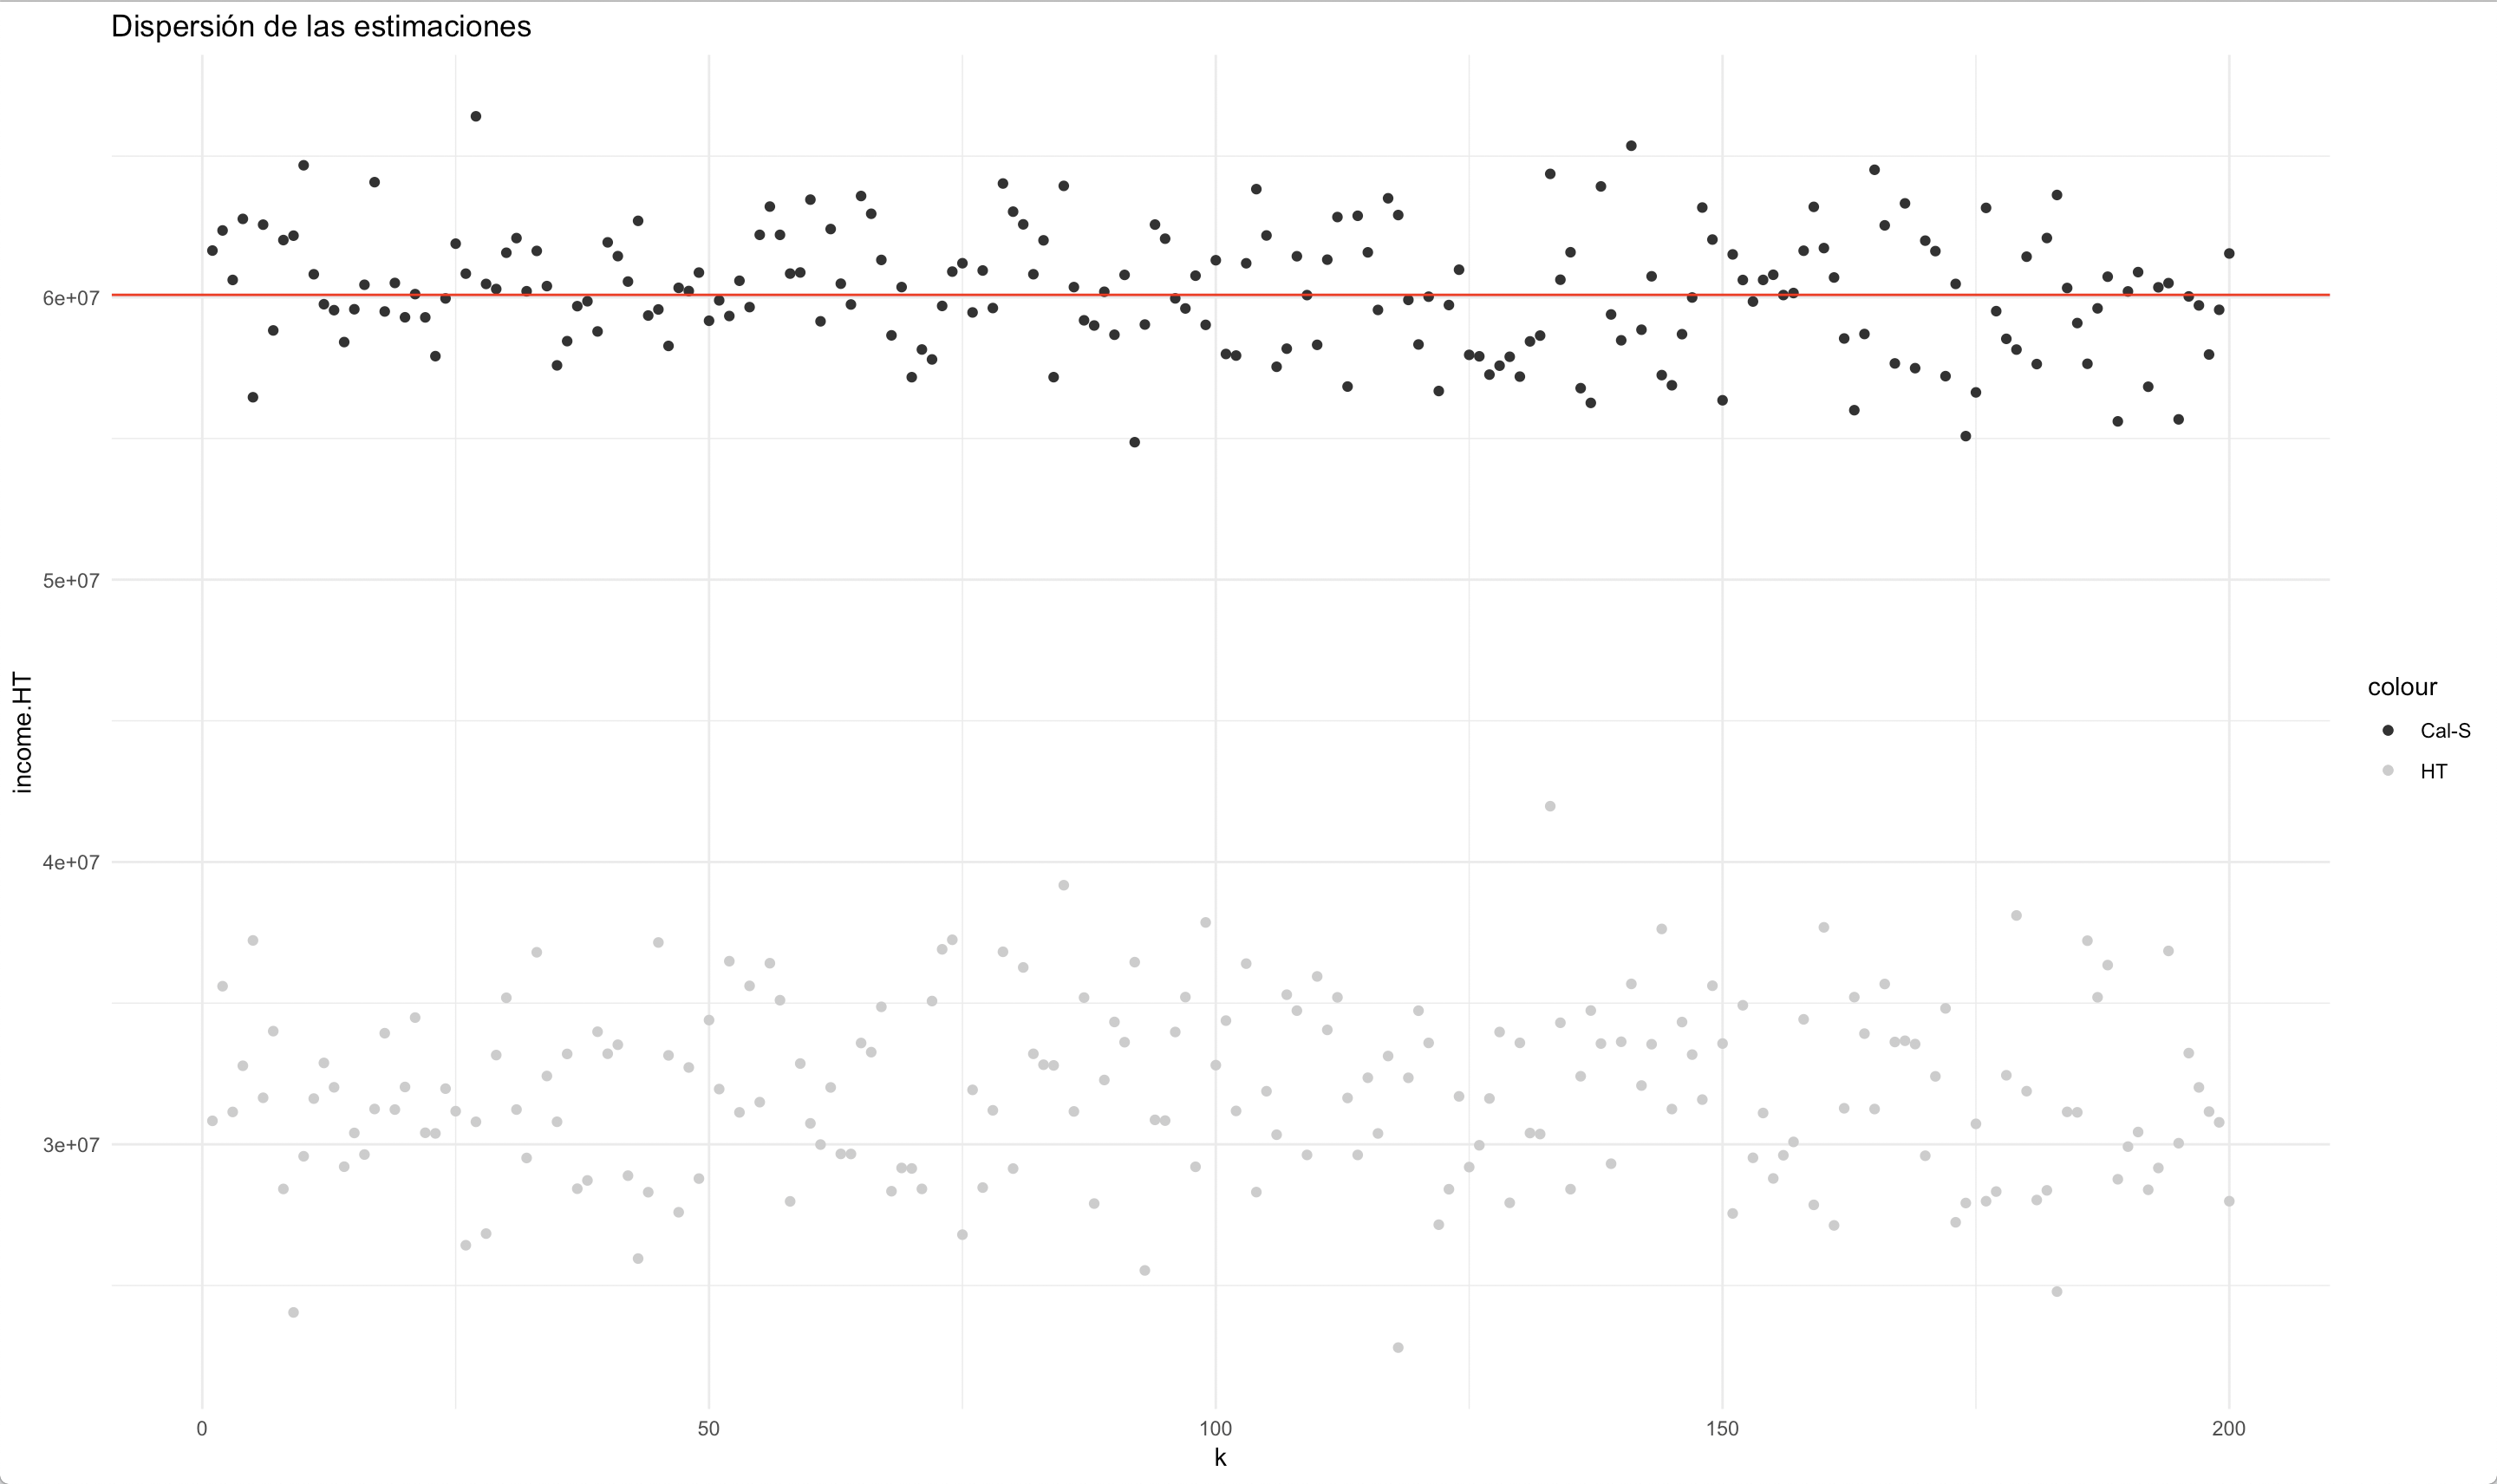
\includegraphics{Pics/c9.png}
\caption{\emph{Estimaciones de Horvtiz-Thompson y de calibración}}
\end{figure}

En conjunto con la gráfica anterior, la siguiente figura muestra la distribución sesgada del estimador de Horvitz-Thompson (gris) en comparación con el insesgamiento del estimador de calibración (negro). Bajo este esquema de respuesta, incluir en la calibración las variables pertinentes corrige el sesgo generado por la ausencia de respuesta. En particular, el estimador ingenuo mostró sesgo en los tamaños estimados de hombres y mujeres, en el tamaño estimado de la población, en los ingresos estimados de hombres y mujeres y en los ingresos estimados de la población.

\begin{figure}
\centering
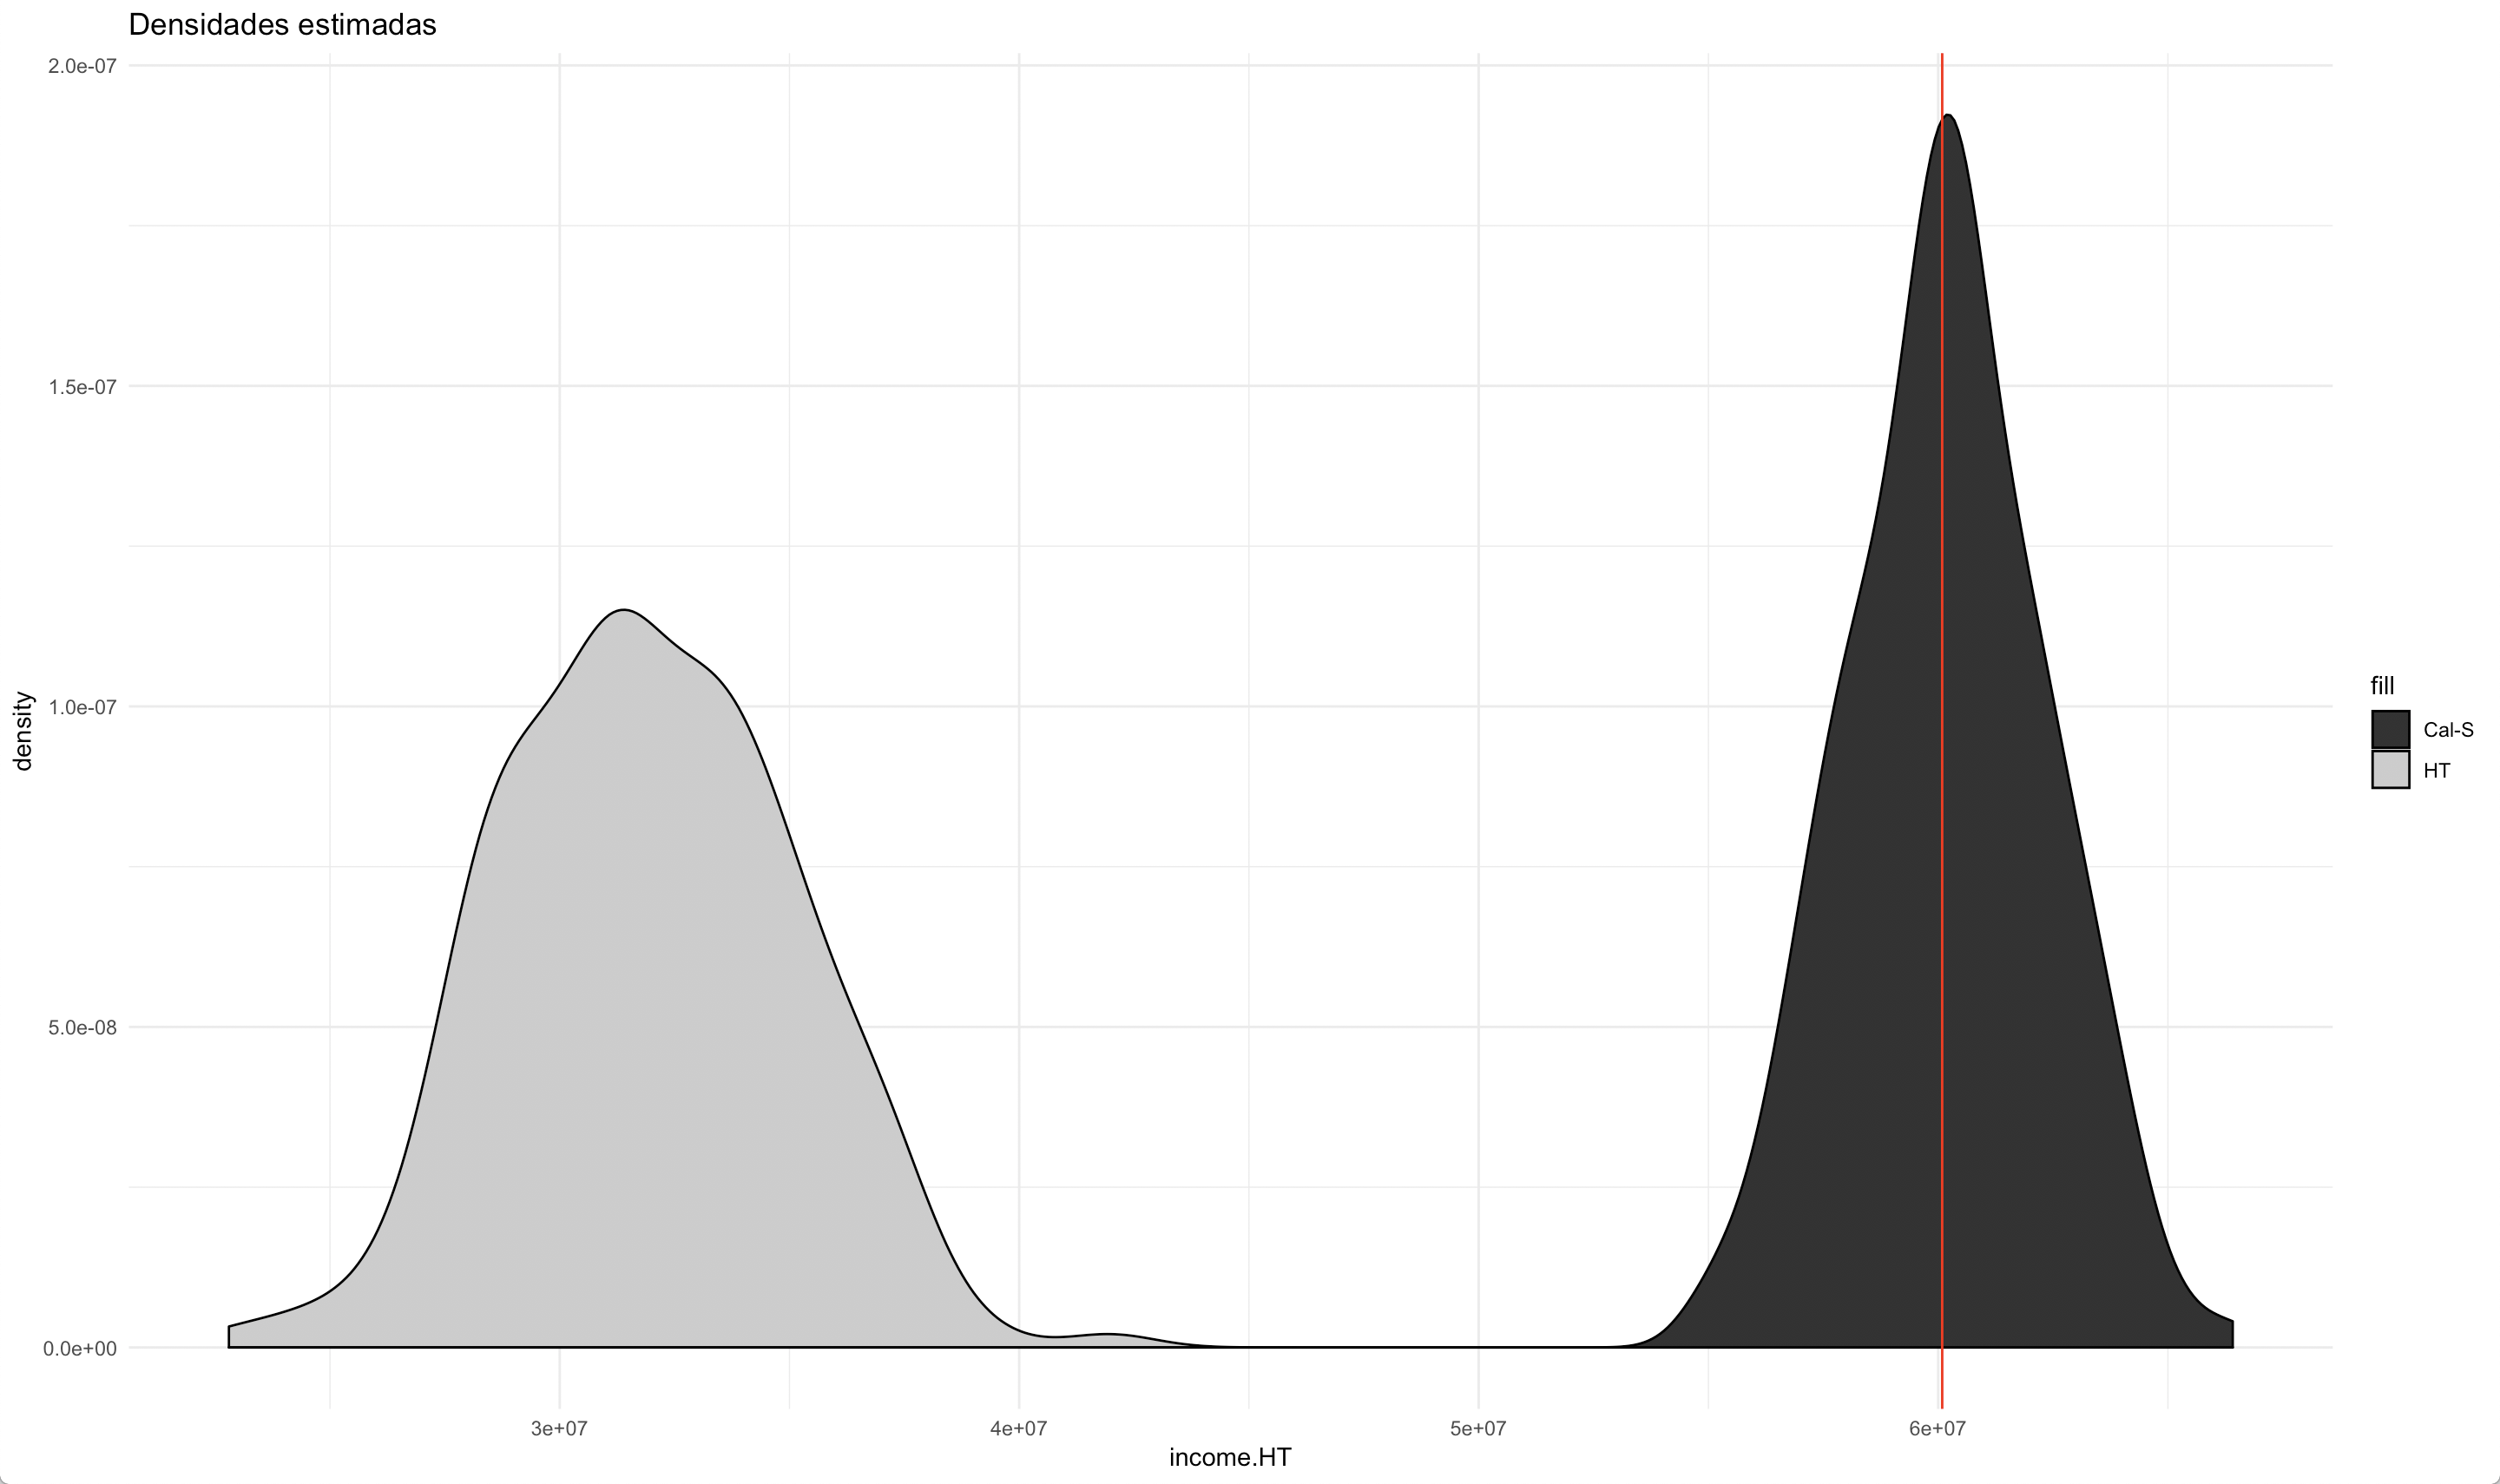
\includegraphics{Pics/c10.png}
\caption{\emph{Distribuciones del estimador de Horvtiz-Thompson y del estimador de calibración}}
\end{figure}

Como se mencionó anteriormente, hay mejores formas de calibrar, puesto que el problema de la calibración se reduce a cómo introducir la información auxiliar en la estructura de estimación de la encuesta, es posible que existan variables que reduzcan el sesgo, pero no todas las variables inducirán el mismo nivel de precisión. Al momento de escoger, se deberían seleccionar aquellas variables que reduzcan el sesgo y que además reduzcan la varianza. Por tanto, las variables auxiliares que se usen como insumo en los procesos de calibración deben:

\begin{itemize}
\tightlist
\item
  Ser capaces de explicar la variación de la probabilidad de respuesta.
\item
  Estar correlacionadas con las variables de interés.
\item
  Identificar los dominios de estimación más importantes.
\end{itemize}

En particular al introducir otras covariables en la calibración (grupo de edad, escolaridad, región, área), además de la corrección del sesgo se evidencia un aumento de la precisión en las nuevas estimaciones, tal como lo muestra las distribuciones de los estimadores en la siguiente figura, en donde se consideran tres estimadores: el estimador de Horvitz-Thompson (gris claro), el estimador de calibración con restricción de sexo (negro) y el estimador de calibración con todas las restricciones (gris oscuro).

\begin{figure}
\centering
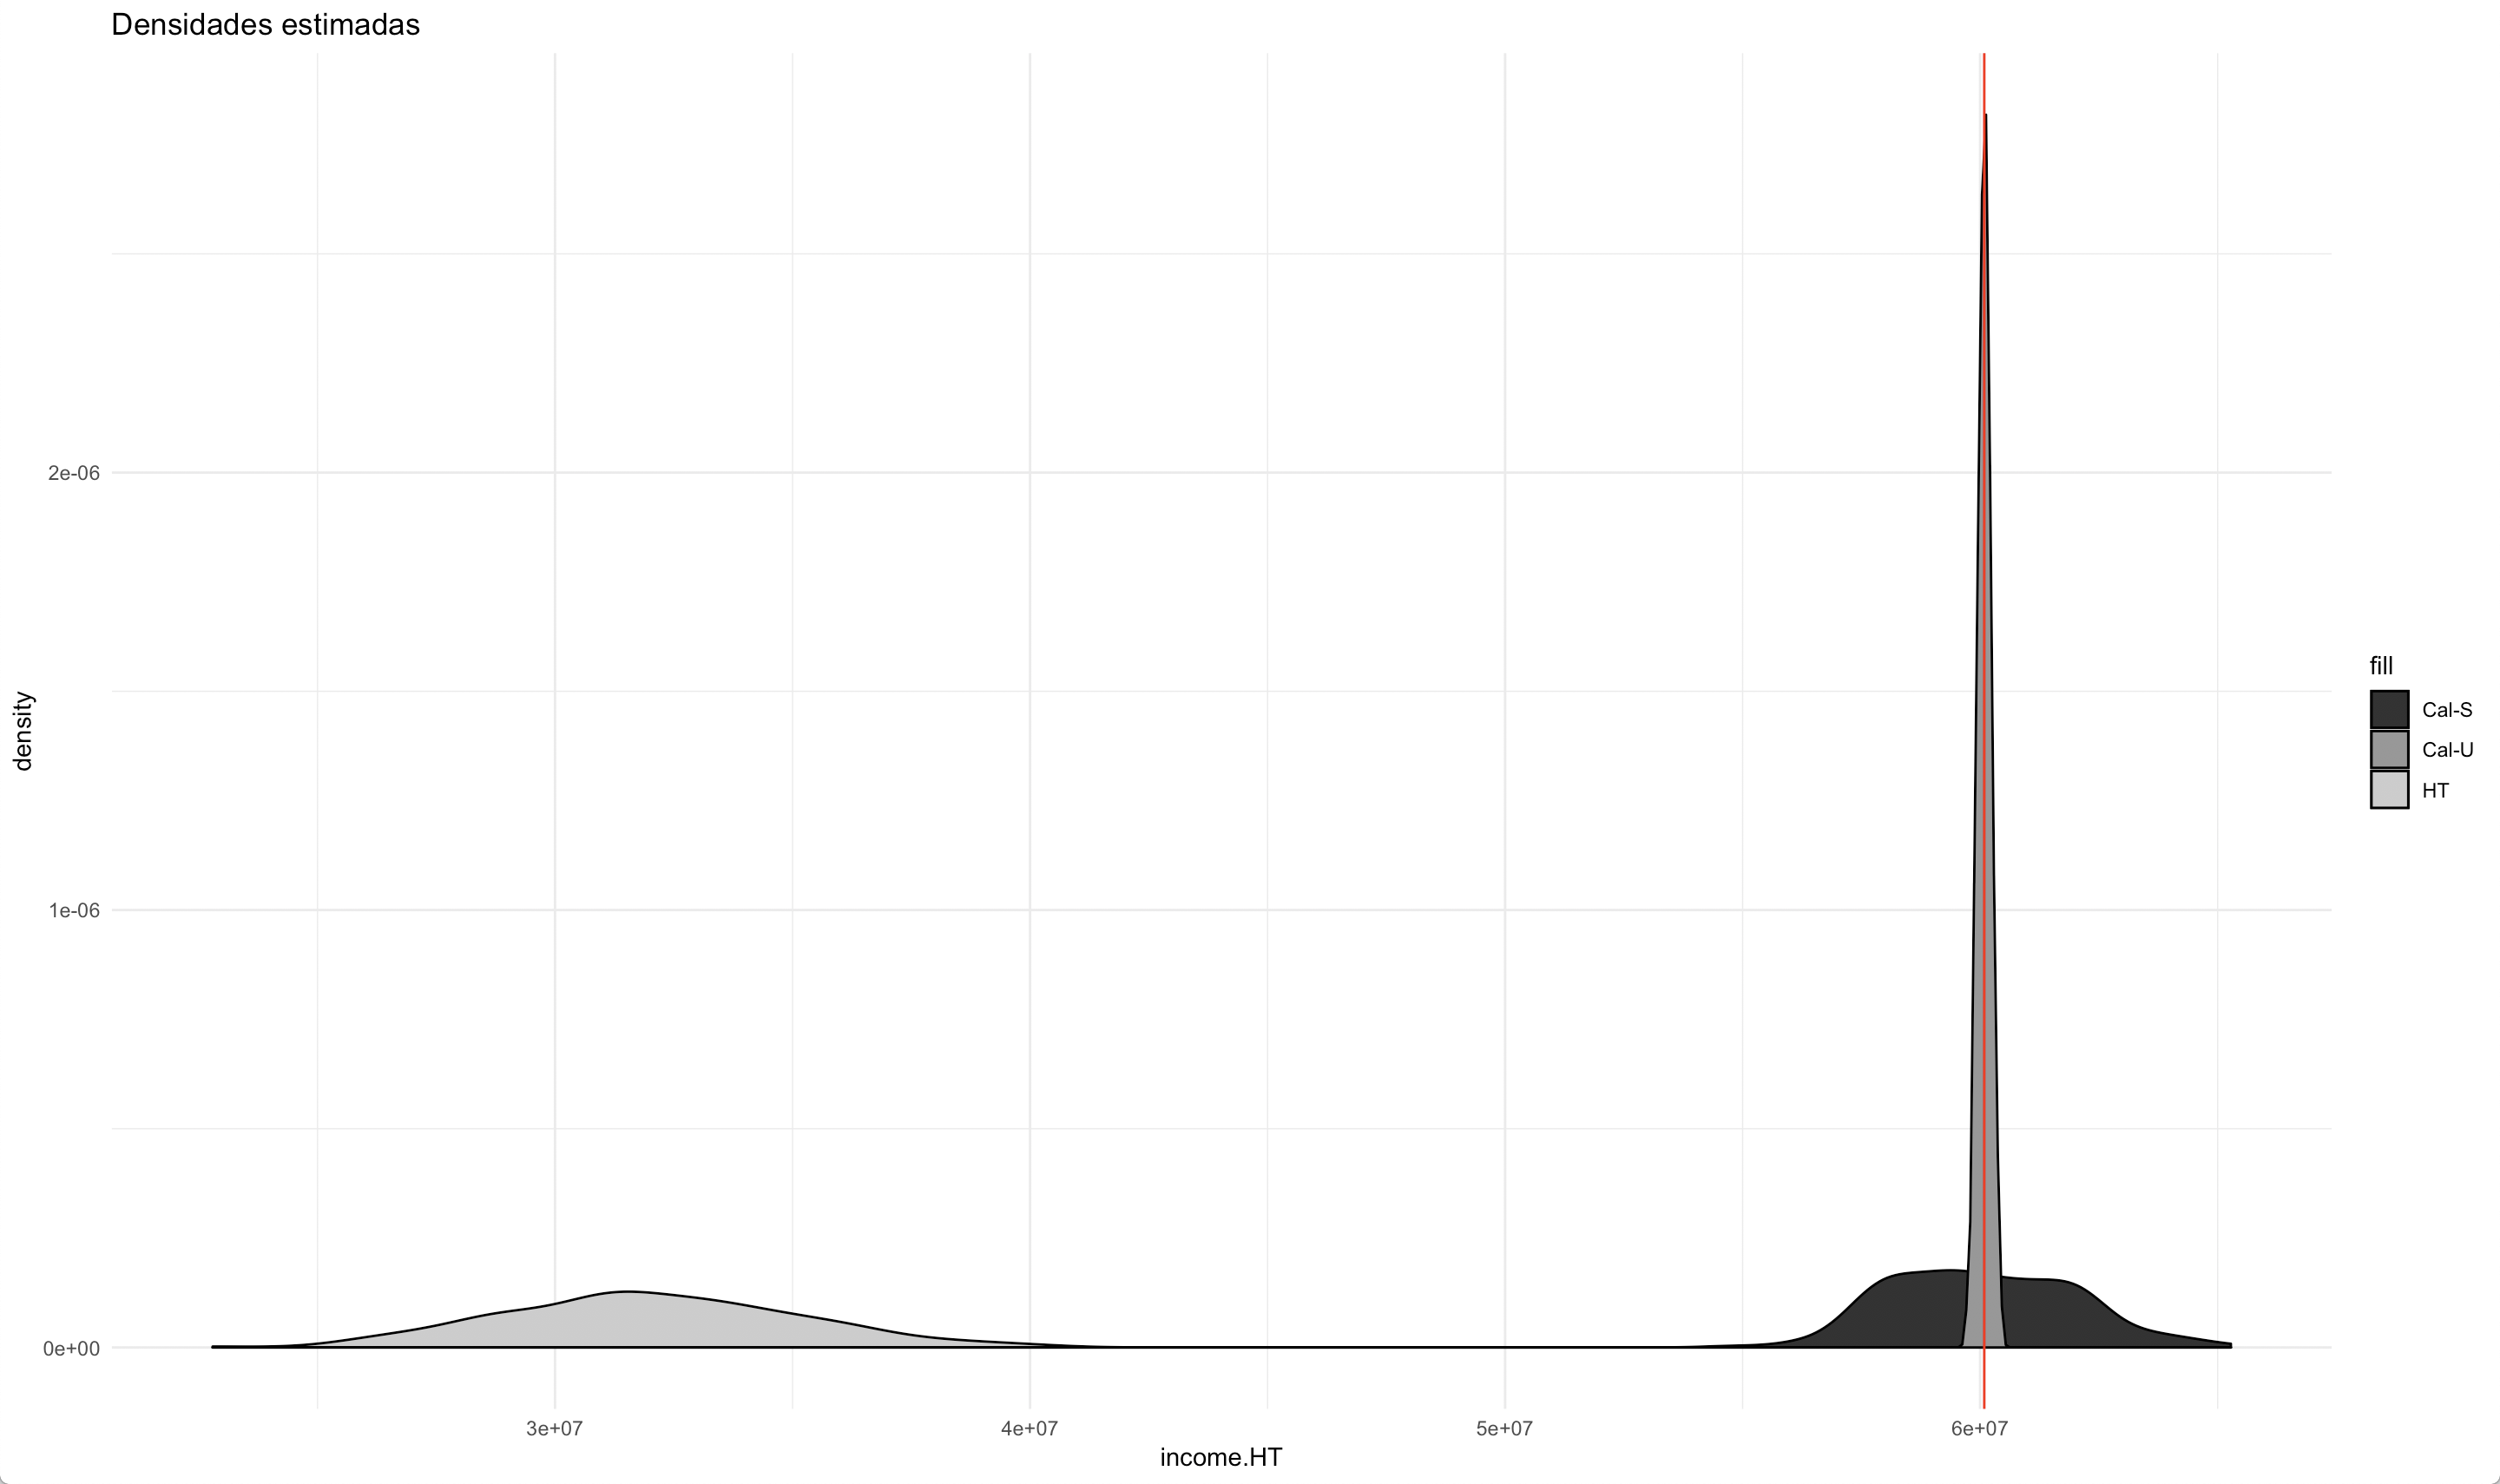
\includegraphics{Pics/c12.png}
\caption{\emph{Distribuciones del estimador de Horvtiz-Thompson y de dos estimadores de calibración}}
\end{figure}

\hypertarget{la-pandemia-por-covid-19-y-la-ausencia-de-respuesta-por-unidad}{%
\section{La pandemia por COVID-19 y la ausencia de respuesta por unidad}\label{la-pandemia-por-covid-19-y-la-ausencia-de-respuesta-por-unidad}}

En su intento por frenar la velocidad de contagio del COVID-19, los gobiernos de la región determinaron la imposición de restricciones de movilidad que truncaron la recolección presencial de las encuestas de hogares. Para hacer frente a este inconveniente y poder seguir produciendo estadísticas oficiales pertinentes y oportunas, la mayoría de INE en la región decidieron realizar el seguimiento continuo a un panel seleccionado de un periodo reciente y mediante contacto telefónico seguir con la recolección de la información primaria. Uno de los retos más importantes que esta pandemia le impuso a las oficinas nacionales de estadística es la corrección del sesgo de selección en las encuestas de hogares. A pesar de los ingentes esfuerzos que se hacieron por minimizarlo durante la recolección, lo cierto es que cambiar de un modo presencial a un modo telefónico trae consigo consecuencias indeseadas que se pueden enfrentar con algunas de las metodologías que se explicaron en esta sección.

Es cierto que es un buen punto de partida para las ONE poder contar con una muestra probabilística de meses anteriores y conformar con ella un panel de seguimiento durante el periodo en el que se tengan estas restricciones de movilidad. En términos de notación, llamémosla la muestra maestra. Sin embargo, se debe tener en cuenta los siguientes dos aspectos importantes:

\begin{enumerate}
\def\labelenumi{\arabic{enumi}.}
\tightlist
\item
  No todos los hogares seleccionados de forma probabilística proveyeron su información de contacto telefónico.
\item
  No todos los hogares contactables respondieron el cuestionario de la encuesta.
\end{enumerate}

Haciendo cálculos gruesos, si suponemos que la cobertura de la submuestra que sí proveyó datos de contacto asciende al 85 \% y que la probabilidad de que un hogar contactado responda toda la encuesta es del 80 \%, entonces contaríamos solamente con un 68\% de la muestra original. A estas cuentas habría que ajustarlas con el efecto de la atrición en el panel, que crece a medida que se siga utilizando. En estos términos, sería un grave error y una suposición poco plausible asumir que los hogares respondientes efectivos se comportan de manera similar a los hogares no respondientes y a los hogares no cubiertos. El mejor escenario que pueden plantearse es considerar que la muestra efectiva no está libre de sesgos, hacer una búsqueda exploratoria de su magnitud con los datos recolectados y tratar de minimizarlo (o incluso eliminarlo) utilizando alguna de las técnicas estadísticas que mencionamos en este documento.

La figura 1 presenta tres posibles escenarios que los INE pudieron encontrar en esta búsqueda. En el diagrama de la izquierda se verifica la ausencia de sesgo, en el diagrama del centro y en el de la derecha se confirma que la magnitud del sesgo es significativa. Nótese que la línea horizontal azul correspondería a la estimación publicada en el mes en el que se seleccionó la muestra maestra, mientras que la línea roja horizontal representa el promedio de las simulaciones con la muestra efectiva. Cada uno de los resultados de las simulaciones está representado por las fluctuaciones punteadas.

\begin{figure}
\centering
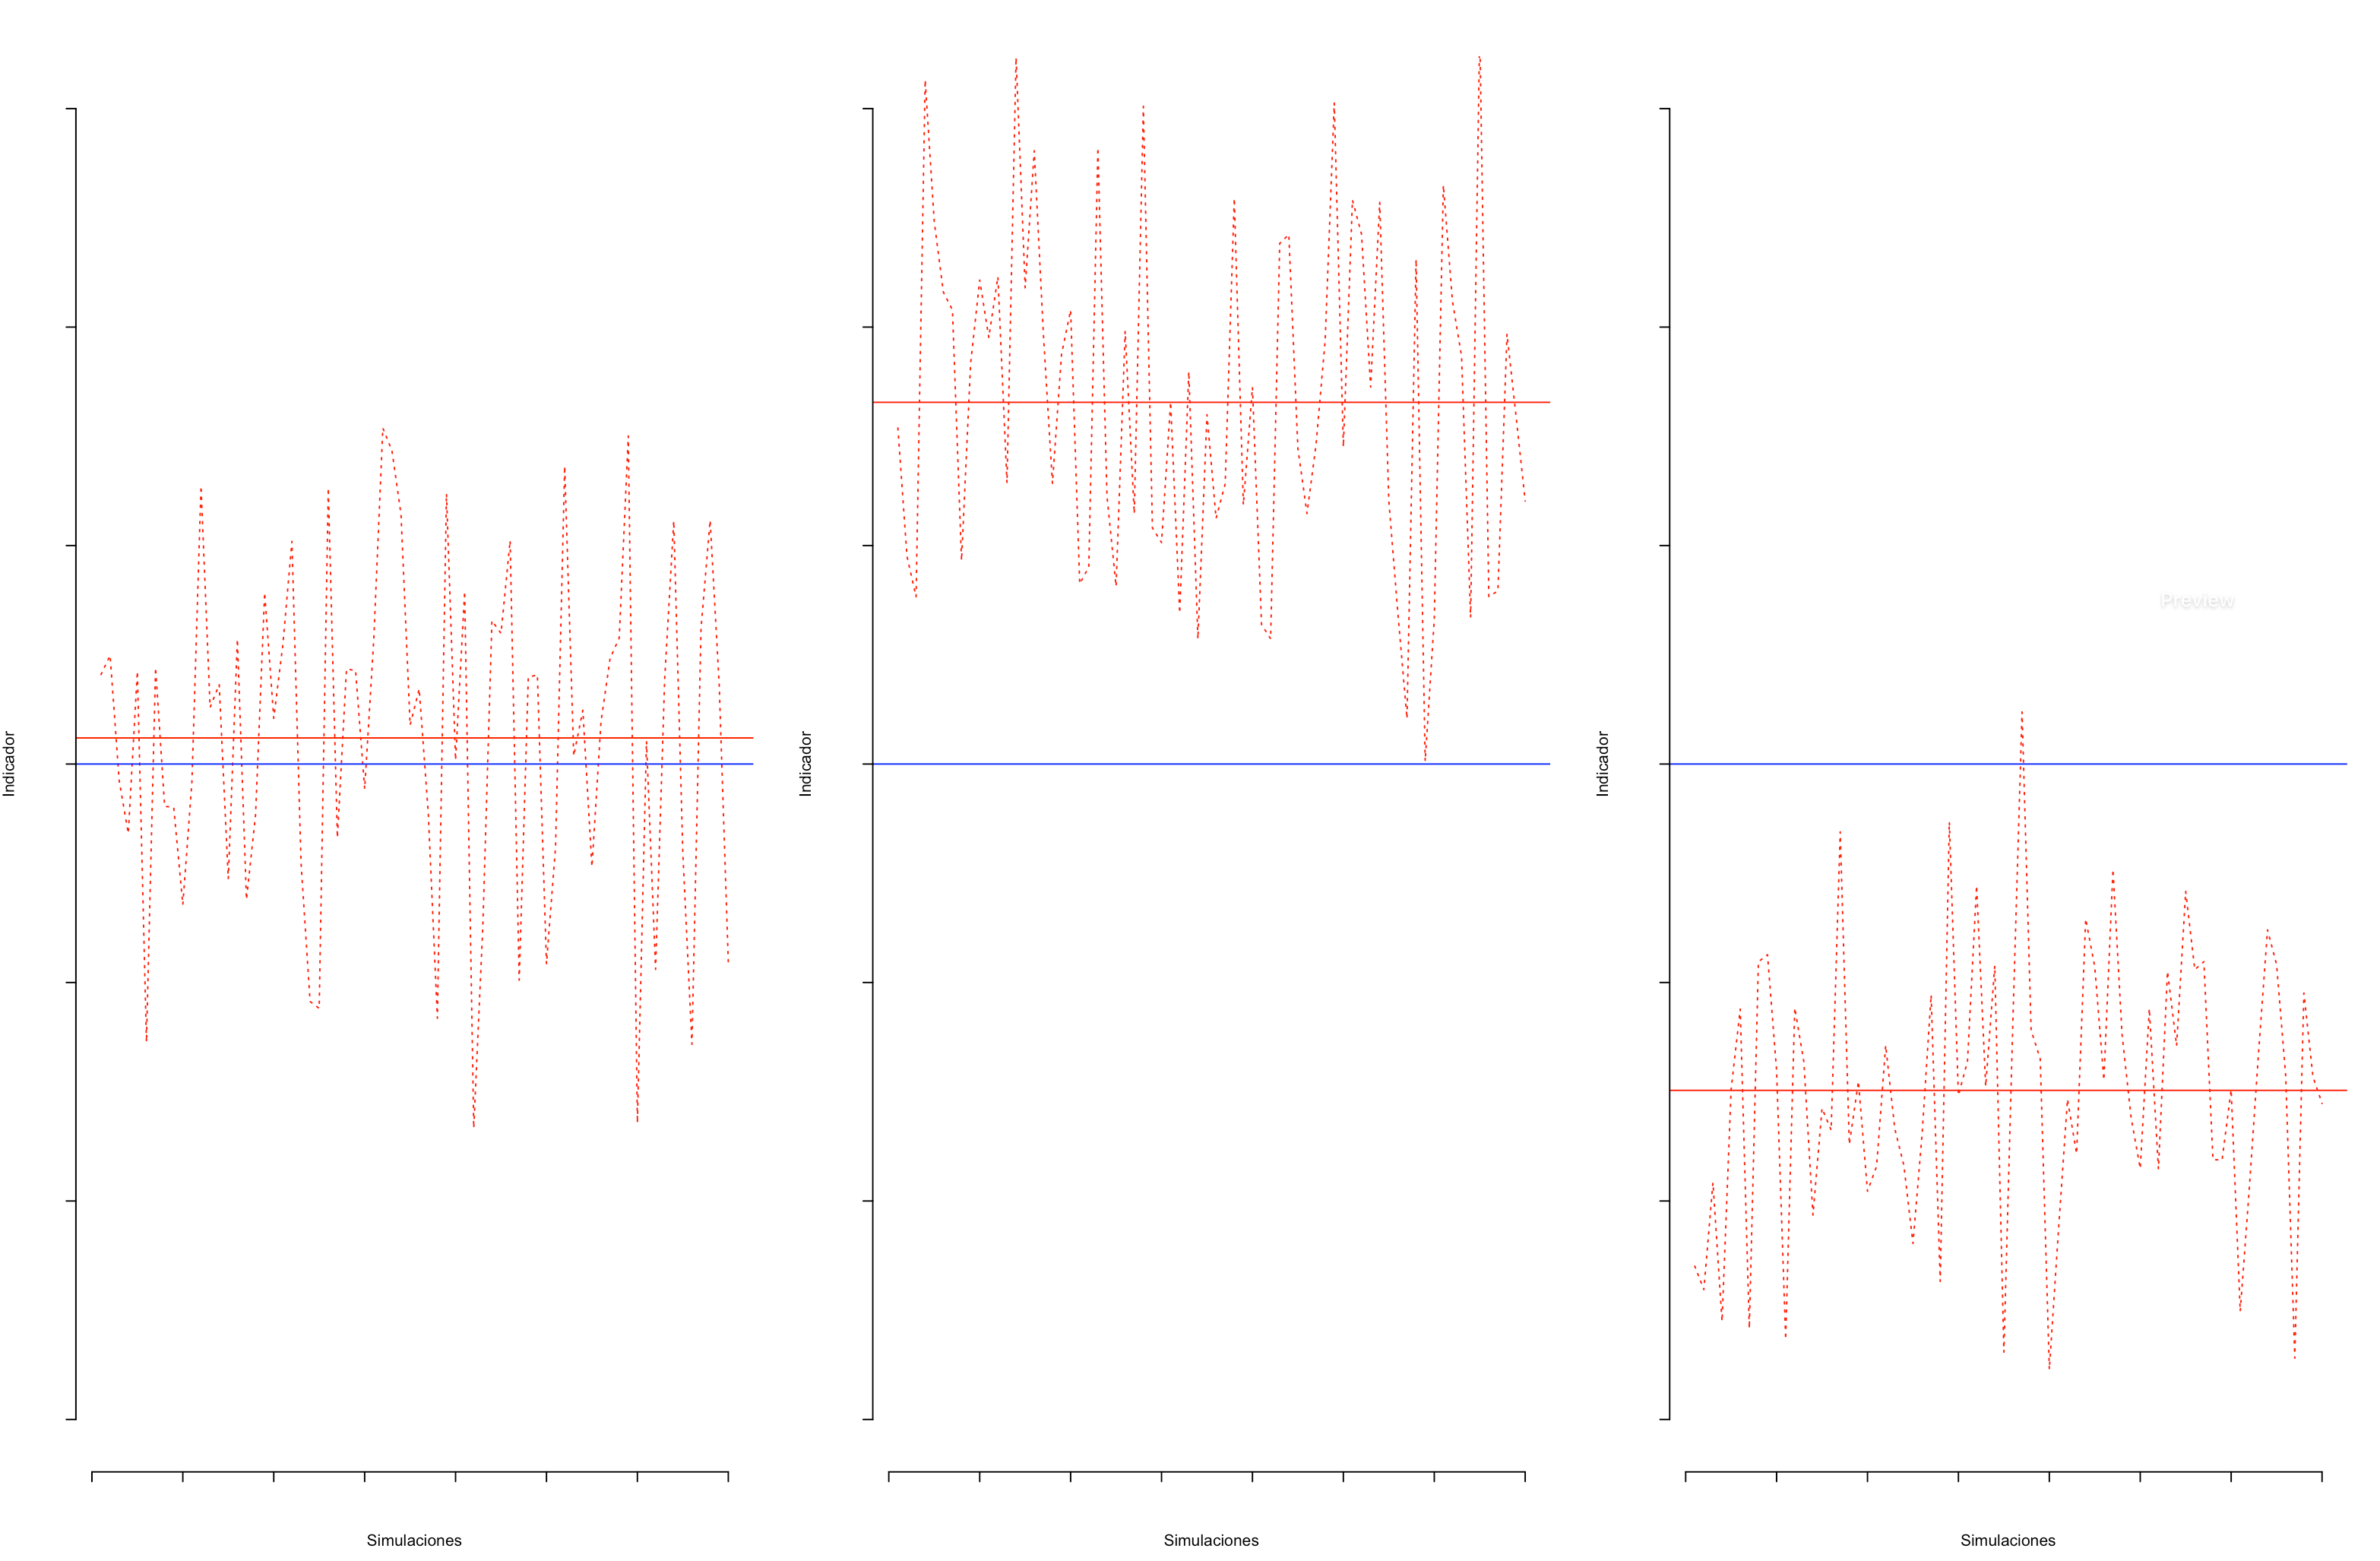
\includegraphics{Pics/calnr1.png}
\caption{\emph{Distribuciones del estimador de Horvtiz-Thompson y de dos estimadores de calibración}}
\end{figure}

La siguiente figura muestra un escenario simulado en donde se contempla el uso del estimador ajustado con la técnica de \emph{propensity score} (línea verde) y el estimador de calibración en dos etapas (línea azul) comparado con el estimador sin ningún tipo de ajuste (línea negra). Lo que se esperaría es que es estimador ingenuo subestime los tamaños poblacionales y los indicadores de interés; mientras que los estimadores ajustados, siempre que el mecanismo de ausencia de respuesta sea MAR o MCAR, elimina este sesgo.

\begin{figure}
\centering
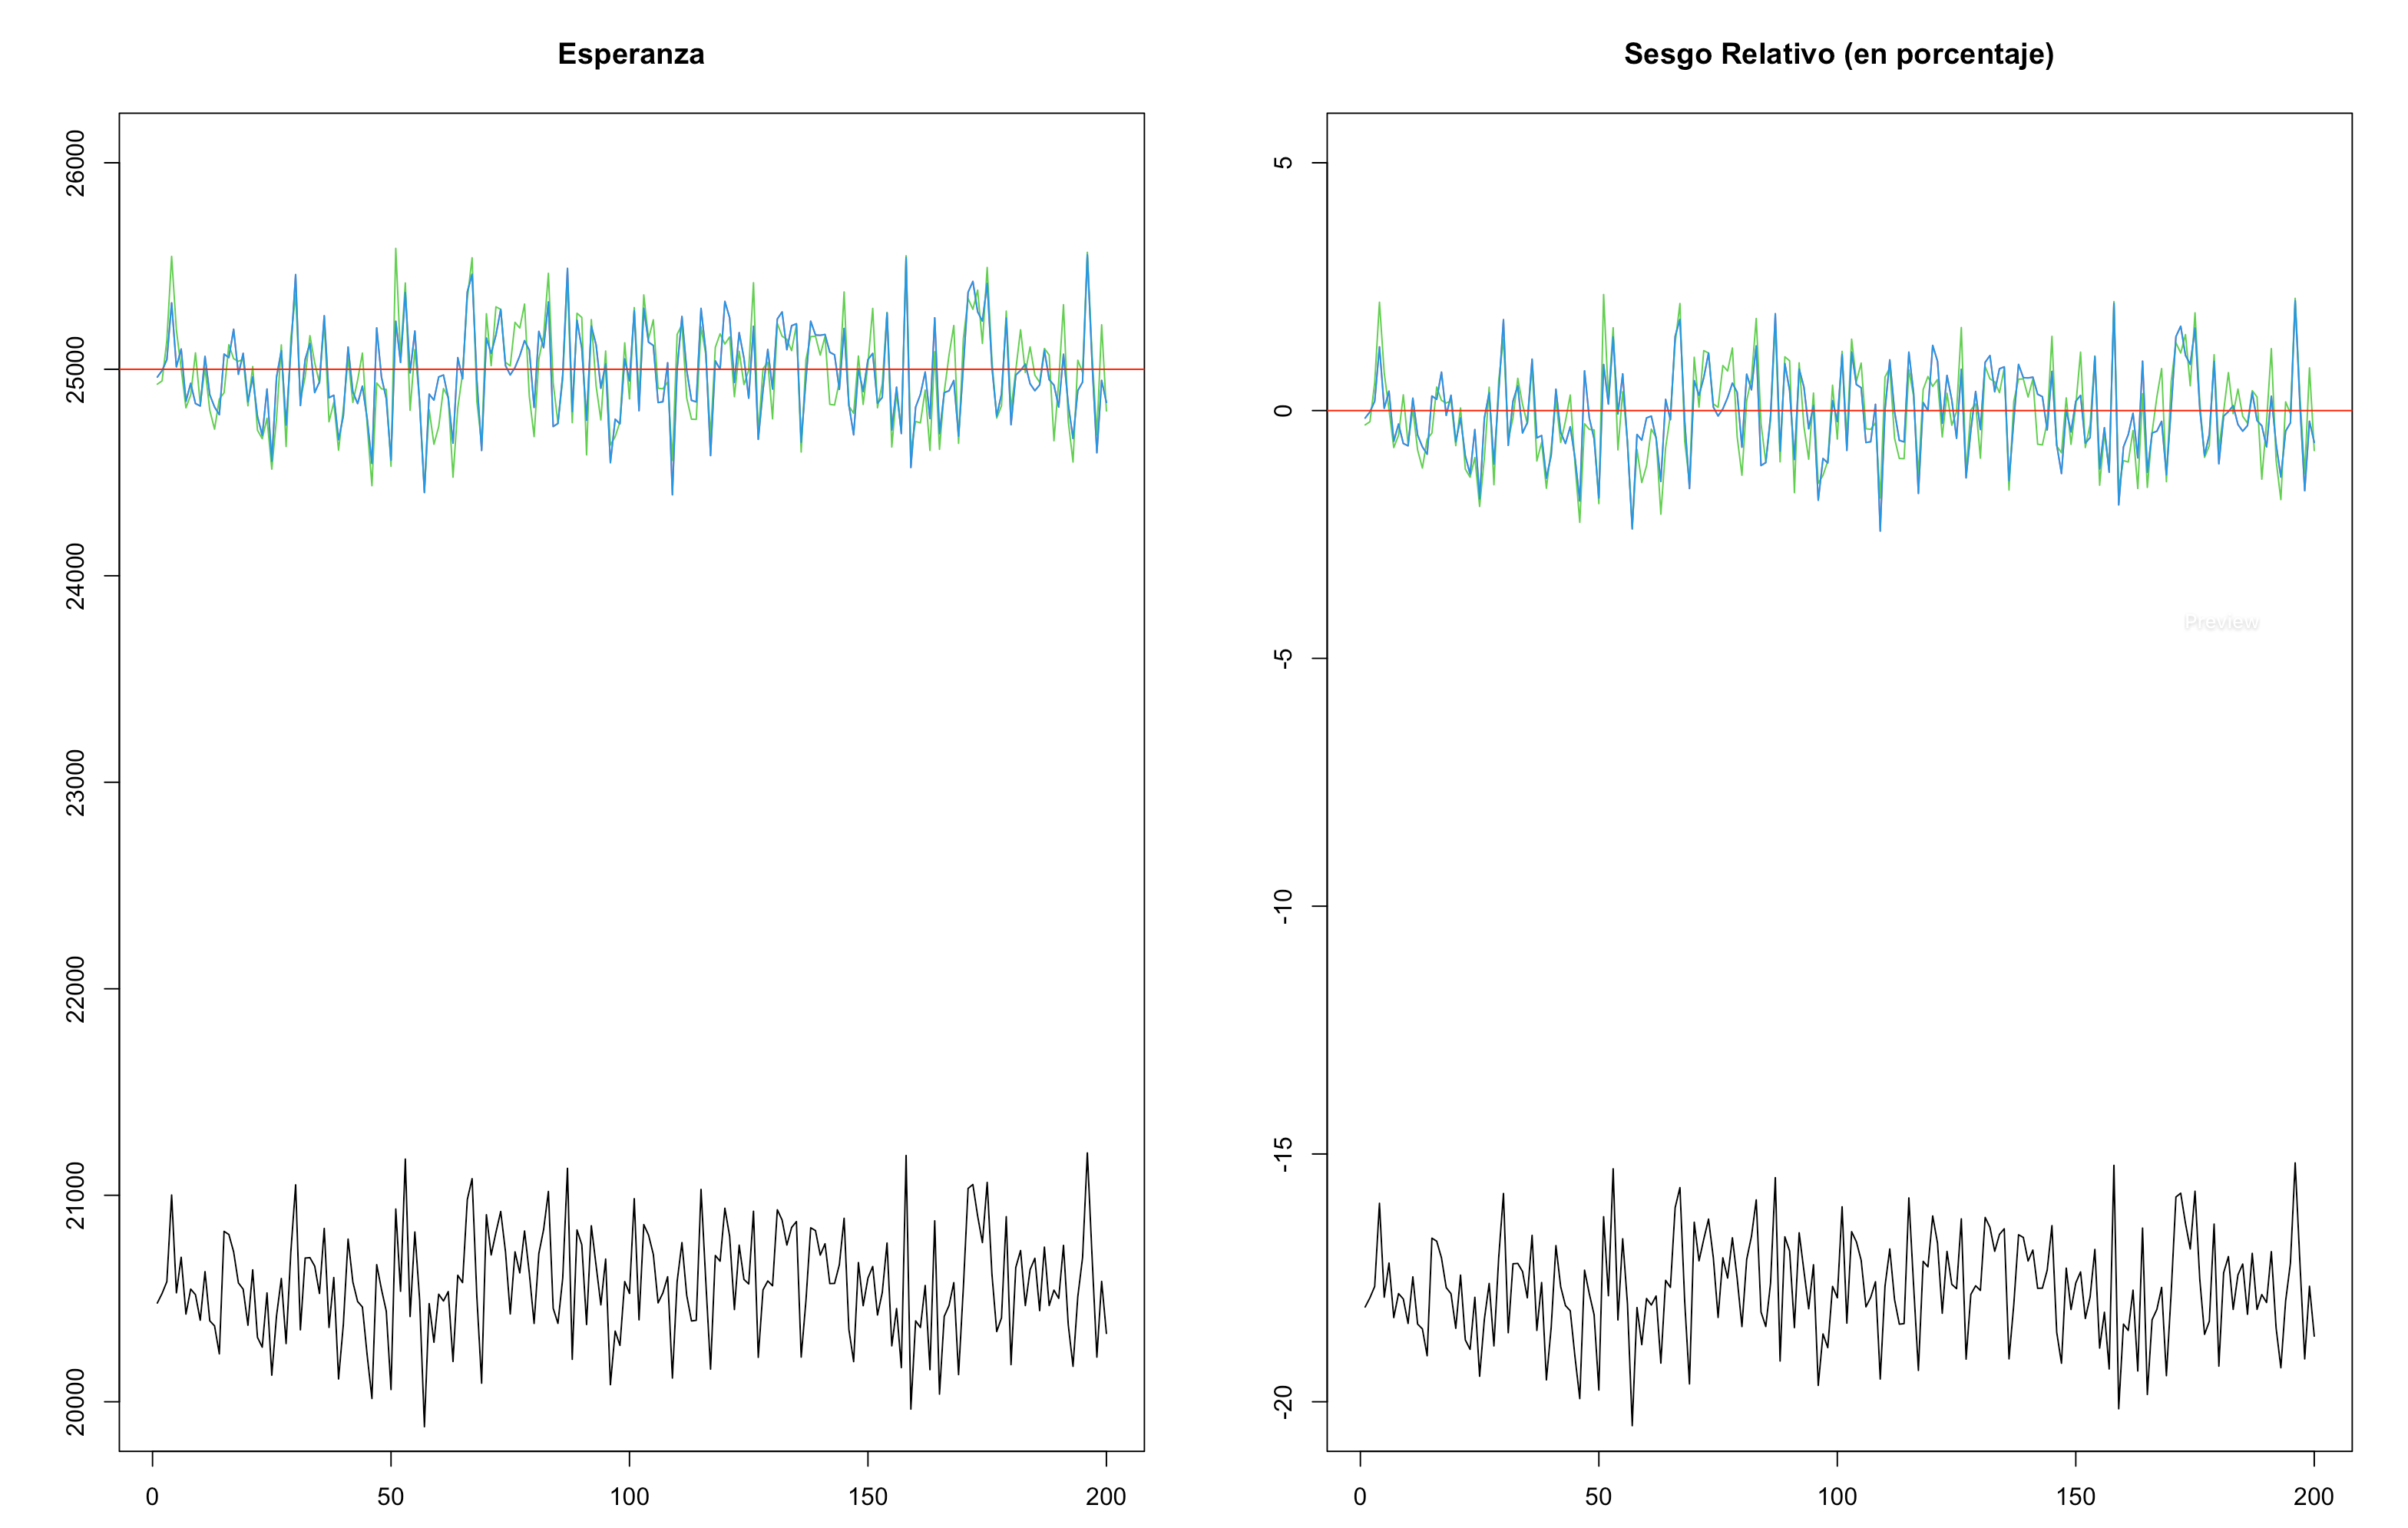
\includegraphics{Pics/calnr2.png}
\caption{\emph{Distribuciones del estimador de Horvtiz-Thompson y de dos estimadores de calibración}}
\end{figure}

Los caminos que se deben seguir luego de corroborar la presencia (o ausencia) de sesgo dependerán de la estrategia de levantamiento de información que los países hayan decidido hacer. En el escenario más optimista, ante la ausencia de sesgo, la ONE estaría en una buena posición para replicar los procesos usuales de inferencia. Sin embargo, si se sospecha de que sí existe sesgo, y dependiendo de la información auxiliar disponible, los INE pudieron disponer de las alternativas que se describen a continuación.

\hypertarget{propensity-score-1}{%
\subsubsection*{Propensity score}\label{propensity-score-1}}
\addcontentsline{toc}{subsubsection}{Propensity score}

Como se mencionó anteriormente, muchos países de la región decidieron realizar un seguimiento mensual telefónico a la muestra maestra como alternativa a las restricciones de movilidad que se han impuesto en los países y que impiden la recolección presencial de la información. En este caso, partiendo de una muestra probabilística se pueden realizar ajustes a los factores de expansión de manera diferencial.

En particular, tener una muestra maestra para la cual se obtuvo toda la información del cuestionario en un periodo anterior constituye un excelente punto de partida para tratar de eliminar el sesgo, puesto que se tendrá acceso a todo un conjunto de covariables \(\mathbf{x}\) que determinarán el mejor modelo para estimar el patrón de ausencia de respuesta en la muestra de respondientes efectivos.

En este paso se debe asumir que la probabilidad de respuesta depende de alguna combinación lineal de las covariables en la muestra maestra; es decir que el mecanismo que genera esa ausencia de respuesta se puede describir mediante \(\mathbf{x}\). Teniendo en cuenta que los pesos originales de la encuesta telefónica se denotan como \(d_k\), y habiendo estimado \(\hat\phi_{k}\) para respondientes y no respondientes de la muestra telefónica, entonces el factor de expansión ajustado tomaría la siguiente forma

\[
w_k = \frac{d_k}{\hat{\phi}_k}
\]

En este sentido, utilizar el factor de expansión \(w_k\) minimizaría el sesgo de selección que se generó por el cambio de modo en la recolección de la información. Por ejemplo, podríamos considerar que un buen modelo de \emph{propensity score} contemplase la edad, el nivel educativo, el área de residencia (rural/urbano), el sexo del respondiente, la región geográfica, el estado de ocupación en el mes de observación de la muestra maestra y el ingreso percápita del hogar. Nótese que todas las covariables en el modelo, salvo el área y la región geográfica, necesariamente provienen de las observaciones obtenidas en la muestra maestra.

\hypertarget{calibraciuxf3n-en-dos-etapas}{%
\subsubsection*{Calibración en dos etapas}\label{calibraciuxf3n-en-dos-etapas}}
\addcontentsline{toc}{subsubsection}{Calibración en dos etapas}

La coherencia entre las cifras oficiales ya publicadas y las que la encuesta telefónica puede producir hace que sea preferible el uso de los estimadores de calibración, o al menos que se complemente. Al usar este enfoque se asegura una estructura inferencial robusta en presencia de la información disponible puesto que se reduce tanto el error de muestreo (aumentando la precisión) como el error debido a la ausencia de respuesta (eliminando el sesgo). A manera de ejemplo, podríamos considerar que la siguientes dos etapas de la calibración son suficientes para eliminar el sesgo generado por el cambio de modo de recolección:

\begin{itemize}
\tightlist
\item
  En la primera etapa se calibran los pesos de la muestra maestra usando las variables de edad, región, área y sexo, definidas convenientemente en en \(\boldsymbol{x}_{1k}\). Los totales de estas variables se encuentran en los conteos censales o en su defecto, en las proyecciones demográficas.
\item
  En una segunda etapa se calibrarán los pesos de la muestra telefónica usando las anteriores variables \(\boldsymbol{x}_{1k}\) y además las variables de ingreso percápita, condición de ocupación, rama de actividad y escolaridad, definidas convenientemente en en \(\boldsymbol{x}_{2k}\). Los totales de estas variables fueron estimados en la misma publicación de la encuesta basada en la muestra maestra.
\end{itemize}

\hypertarget{referencias}{%
\chapter*{Referencias}\label{referencias}}
\addcontentsline{toc}{chapter}{Referencias}

  \bibliography{CEPAL.bib}

\end{document}
